\documentclass[fontsize=11pt,a4paper,DIV=12]{scrartcl}

% --------------------------------------------------------
% Fonts & Encoding
% --------------------------------------------------------
\usepackage[T1]{fontenc}
\usepackage{libertine}
\def\sc{\scshape}
\def\tt{\ttfamily}

% --------------------------------------------------------
% Math Packages
% --------------------------------------------------------
\usepackage{amsmath, amsthm, amsfonts, amssymb, mathtools, thm-restate, enumerate}

% --------------------------------------------------------
% Graphics, Colors, & TikZ
% --------------------------------------------------------
\usepackage{xcolor, mycolor, graphicx, tikz}
\usetikzlibrary{backgrounds, 3d, intersections, calc, arrows.meta}

% --------------------------------------------------------
% Floats & Figures
% --------------------------------------------------------
\usepackage[section]{placeins}
\usepackage{etoolbox}
% Automatically add a FloatBarrier before every subsection
\pretocmd{\subsection}{\FloatBarrier}{}{}

\usepackage[subrefformat=simple,labelformat=simple]{subcaption}
\renewcommand\thesubfigure{(\textsc{\alph{subfigure})}}

% --------------------------------------------------------
% Utilities
% --------------------------------------------------------
\usepackage{xspace, xstring}
\usepackage{needspace}
\setlength{\emergencystretch}{2em}

% --------------------------------------------------------
% Bib
% --------------------------------------------------------
\usepackage[
  backend=biber,
  style=alphabetic,
  sortcites=true,
  sorting=ynt,
  maxbibnames=99,
  maxcitenames=99,
  minalphanames=3,
  giveninits=true,
  backref=true,
  doi=true,
  isbn=false,
  url=false,
  eprint=true
]{biblatex}

% Point to your .bib file
\addbibresource{bib.bib}

% --------------------------------------------------------
% Hyperlinks & Cross-Referencing (Keep at the very end)
% --------------------------------------------------------
\usepackage{hyperref}
\hypersetup{colorlinks=true, citecolor=Blue, linkcolor=Blue, urlcolor=Blue}
\usepackage[noabbrev,capitalise]{cleveref}

% --------------------------------------------------------
% Custom Commands & Environments
% --------------------------------------------------------

% emphasis of a definition
\newcommand{\defn}[1]{\textsl{\textcolor{Blue}{#1}}}
% theorems
\let\theorem\relax
\newtheorem{theorem}{Theorem}
\newtheorem{observation}[theorem]{Observation}
\newtheorem{claim}[theorem]{Claim}
\newtheorem{remark}[theorem]{Remark}
\newtheorem{conjecture}[theorem]{Conjecture}
\newtheorem{lemma}[theorem]{Lemma}
\newtheorem{proposition}[theorem]{Proposition}
\newtheorem{corollary}[theorem]{Corollary}
\newtheorem{definition}[theorem]{Definition}

% commands
\newcommand{\fh}{facet-Hamil\-tonian\xspace}
\newcommand{\kernel}{kernel\xspace}
\newcommand{\inv}{^{-1}}
\DeclareMathOperator{\RR}{\mathbb{R}}
\DeclareMathOperator{\N}{\mathbb{N}}
\DeclareMathOperator{\tr}{tr}

\makeatletter
\def\@fnsymbol#1{%
   \ifcase#1
   \or A
   \or B
   \or F
   \or K
   \or L
   \or X
   \else
   \@ctrerr \fi
}%
\makeatother

\DeclareTOCStyleEntry[
    indent=0em,
    pagenumberformat=\normalfont,
    beforeskip=1pt plus .2pt,
    entryformat=\normalfont
    ]{tocline}{section}

% this is a fix for annoying errors when reusing names for boxes in auto generated tikz code
\let\oldnewsavebox\newsavebox
\renewcommand{\newsavebox}[1]{%
  \ifdefined#1%
    % Silently ignore
  \else
    \oldnewsavebox{#1}%
  \fi
}

    \newcommand{\anonymous}{N} %set to Y for anonymous version
\begin{document}

\title{\huge Rhombic Strips of Graded Posets}
\if\anonymous Y{
			\author{}
		}\else
	{
		\author{
			Stefan Felsner\,\thanks{Technische Universit\"at Berlin, Germany, felsner@math.tu-berlin.de} \and
			Robert Lauff\,\thanks{Technische Universit\"at Berlin, Germany, lauff@math.tu-berlin.de}
		}
	}
\fi

\date{}

\maketitle
\vspace{-30pt}
\begin{abstract}
	\noindent{\textbf{Abstract.}}
	Rhombic strips are a class of plane
	spanning sub-diagrams of graded posets.
	They were introduced by Akitaya, Cardinal, Felsner,
	Kleist, and Lauff to encode facet-Hamiltonian paths and
	cycles on polytopes (SODA25). Subsequently, Behrooznia, Brenner,
	Merino, Mütze, Rieck, and Verciani used them to prove a
	conjecture from the first paper about facet-Hamiltonian
	cycles in B-permutahedra (SODA26). We describe
	three constructions for rhombic strips in certain Cartesian
	products of posets. The first two are generalizations of well
	known concepts in the area of combinatorial Gray codes and Venn diagrams:
	\begin{itemize}
		\item Unfolding --- this technique generalizes the binary reflected Gray code,
		      i.e., the classical Gray code construction for bit strings.
		      A construction for simple monotone Venn diagrams by Edwards 1989
		      can also be described as unfolding rhombic strips.
		\item Zigzagging --- this technique generalizes the Steinhaus-Johnson-Trotter
		      Gray code for permutations. The original construction for Venn diagrams by
		      Venn 1880 can also be described as zigzagging rhombic strips.
	\end{itemize}

	Rhombic strips form a generalized higher
	level structure on which to view these classic constructions.

	Using rhombic strips and unfolding we provide a simple
	construction of Gray codes for combinations
	of multisets. This reproves a result of Ruskey
	and Savage 1996. Using zigzagging we can also
	construct cyclic Gray codes for combinations of
	multisets which contain an element with
	odd multiplicity; this resolves most cases of a conjecture of
	Ruskey and Savage 1996. Adapting this construction also resolves the remaining case in which all multiplicities are even, fully resolving the conjecture.

	Zigzagging also allows us to reprove that the restriction of the
	Steinhaus-Johnson-Trotter Gray code to permutations
	with a fixed number of inversions yields a Gray code for these permutations, which is a result of Vajnovszki and Vernay.

	Combining unfolding and zigzagging we show that a product of posets admits a
		rhombic strip if one poset admits a Hamiltonian rhombic strip and the other
		admits a non-cyclic rhombic strip.  This technique is used for a construction of
	facet-Hamiltonian paths and cycles on graph associahedra of trees, and greatly extends results from the SODA25 paper,
	which were restricted to caterpillars, and only yielded facet-Hamiltonian paths, not cycles. The
	rhombic strip used in the construction is Hamiltonian; this yields a Gray code for all rooted subtrees of a
	given base tree.  Moreover, restricting the Hamiltonian path to subtrees with
	a fixed number of vertices, we obtain a Gray code.
\end{abstract}

\thispagestyle{empty}

\setcounter{page}{1}

\pagebreak

\section{Introduction} \label{sec:intro}

The generation of combinatorial objects, such as subsets, permutations, multisets, and trees, is a foundational problem in theoretical computer science and combinatorics. Often, an efficient algorithm can apply minimal structural changes to generate the next object. Such a listing in which adjacent objects are minimally different is known as a \defn{Gray code}, see \cite{survey_gray_codes} for a survey of Gray codes. When viewing the objects of a combinatorial family as the vertices of a graph, and the minimal changes as edges in that graph, we obtain what is known as a \defn{flip graph}. The challenge then becomes finding a Hamilton path or cycle in this flip graph. These flip graphs are often very structured. For example, when listing permutations by adjacent transposition, the flip graph is a well studied polytope known as the \defn{permutahedron}. When listing the subsets of a finite ground set by adding or removing single elements, the flip graph is isomorphic to a cube, because the subsets can be viewed as 01-vectors.

When constructing Gray codes inductively, two primary techniques dominate, which we will call \defn{unfolding} and \defn{zigzagging}, respectively. The canonical examples of these methods are the binary reflected Gray code (BRGC) for subsets \cite{GrayCode,KnuthBRGC} and the Steinhaus-Johnson-Trotter (SJT) Gray code for permutations \cite{SJT1,SJT2}, respectively.

The BRGC lists all subsets of $[n]=\{1,\ldots,n\}$. By induction, we obtain a listing of all subsets not containing $n$, then add $n$ to whatever subset comes at the end of this listing, and finally list the subsets of $[n-1]$ in reverse order from before, but keeping $n$ in each of the subsets. This effectively unfolds the listing for subsets of $[n-1]$ into two copies. When viewing the subsets as 01-vectors, this construction generalizes to list all integer vectors of length $n$ in which the $i$-th component is bounded by some given value $b_i$, by unfolding the previous Gray code into $b_n+1$ copies, see \Cref{fig:unfolding explicit} for an example.

\begin{figure}
	\centering
	\newcommand{\brgc}[1]{%
    \begin{tabular}{cccccccc}
        0&0&0&0&1&1&1&1 \\
        0&0&1&1&1&1&0&0 \\
        0&1&1&0&0&1&1&0 \\
        \textbf{#1}&\textbf{#1}&\textbf{#1}&\textbf{#1}&\textbf{#1}&\textbf{#1}&\textbf{#1}&\textbf{#1} 
    \end{tabular}%
}
\newcommand{\brgcinv}[1]{%
    \begin{tabular}{cccccccc}
        1&1&1&1&0&0&0&0 \\
        0&0&1&1&1&1&0&0 \\
        0&1&1&0&0&1&1&0 \\
        \textbf{#1}&\textbf{#1}&\textbf{#1}&\textbf{#1}&\textbf{#1}&\textbf{#1}&\textbf{#1}&\textbf{#1} 
    \end{tabular}%
}

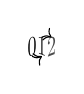
\begin{tikzpicture}

    % 1. The first copy (Slanting UPWARDS)
    \begin{scope}[xscale=0.65, yslant=0.25, transform shape]
        \node[anchor=west, inner sep=0pt] (panel1) at (0,0) {\brgc{0}};
    \end{scope}
    
    % 2. The second copy (Slanting DOWNWARDS)
    % Attaches to the right edge of panel 1
    \begin{scope}[xscale=0.65, yslant=-0.25, transform shape]
        \node[anchor=west, inner sep=0pt, opacity=0.85] (panel2) at (panel1.east) {\brgcinv{1}};
    \end{scope}

    % 3. The third copy (Slanting UPWARDS again)
    % Attaches to the right edge of panel 2
    \begin{scope}[xscale=0.65, yslant=0.25, transform shape]
        \node[anchor=west, inner sep=0pt, opacity=0.7] (panel3) at (panel2.east) {\brgc{2}};
    \end{scope}

    \draw[->] (panel1.south) to[bend right] (panel2.south);
    \draw[->] (panel2.north) to[bend left] (panel3.north);

\end{tikzpicture}
	\caption{Unfolding to obtain a Gray code listing of the 4-dimensional integer vectors with the bounds $(1,1,1,2)$. The vectors are column vectors. Note how the BRGC is repeated 3 times, with 0,1 and 2 appended at the bottom, respectively.}
	\label{fig:unfolding explicit}
\end{figure}

The SJT Gray code lists the set of permutations of $[n]$ by applying adjacent transpositions. However, given the code for permutations of $[n-1]$ by induction, it does not use this listing as is. Rather, it interweaves the new element $n$ in between each flip of the previous listing, putting it in all possible places. The new element $n$ is zigzagging through the old listing. See \Cref{fig:SJT_explicit}.

This idea extends very far. Similar constructions can be used to weave together different Gray codes, and combining this with unfolding allows for creative and powerful proofs. The most general version of zigzagging is probably algorithm J from the seminal series of papers around generating zigzag languages by Mütze et al. \cite{PL1,PL2,PL3,PL4,PL5}. Using so called minimal jumps in permutations, algorithm J can enumerate a large variety of combinatorial objects using a zigzagging construction inspired by SJT.

\begin{figure}
	\centering
	\def\n{\textbf{4}}

\begin{tabular}{cccc|cccc|cccc|cccc|cccc|cccc}
1& 1&1 &\n&\n&1 &1 &1 &3 &3 &3 &\n&\n&3 &3 &3 &2 &2 &2 &\n&\n&2 &2 &2 \\
2& 2&\n&1 &1 &\n&3 &3 &1 &1 &\n&3 &3 &\n&2 &2 &3 &3 &\n&2 &2 &\n&1 &1 \\
3&\n&2 &2 &3 &3 &\n&2 &2 &\n&1 &1 &2 &2 &\n&1 &1 &\n&3 &3 &1 &1 &\n&3 \\
\n&3&3 &3 &2 &2 &2 &\n&\n&2 &2 &2 &1 &1 &1 &\n&\n&1 &1 &1 &3 &3 &3 &\n
\end{tabular}
	\caption{The SJT Gray code for $n=4$. The permutations are column vectors. Note how \textbf{4} is zigzagging through the SJT Gray code for $n=3$.}
	\label{fig:SJT_explicit}
\end{figure}

Going in another direction, these ideas can also be found in the language of \defn{Venn diagrams}. Ignoring the details, a Venn diagram for the subsets of $[n]$ is a collection of $n$ simple closed curves in the plane which cuts it into $2^n$ regions. These regions are then associated to the subsets of $[n]$. The subsets containing $i$ are those regions contained within the $i$'th curve, see also \cite{Survey_Venn} for a survey of Venn diagrams. Two classic constructions of Venn diagrams can be directly related to unfolding and zigzagging, respectively. Morally, these constructions go as follows: Given a Venn diagram $V$ of the subsets of $[n-1]$, place a mirrored copy $\bar{V}$ next to $V$. Cut both copies open and join the curves, then place a new curve around $\bar V$, not intersecting $V$. The regions of $\bar V$ now represent the subsets containing $n$ while the regions of $V$ represent the subsets not containing $n$, and the new curve separates them. One can say that $V$ has been unfolded into two copies of itself. This is the essence of a classical construction by Edwards \cite{Edwards1989}. See \Cref{fig:venn unfolding}.

The original construction by Venn \cite{Venn1880} goes as follows: Say the dual graph of a Venn diagram $V$ for the subsets of $[n-1]$ contains a Hamilton cycle. We can draw this Hamilton cycle as a new curve and add this curve to $V$. This way, each region is split into two new regions, one of which is inside the new curve. The regions inside the new curve then represent subsets containing $n$. One can say that the Hamilton cycle is zigzagging in and out of $V$. See \Cref{fig:venn zigzagging}.

\begin{figure}[htbp]
	\centering
	% Subfigure 1
	\begin{subfigure}[b]{0.48\textwidth}
		\centering
		

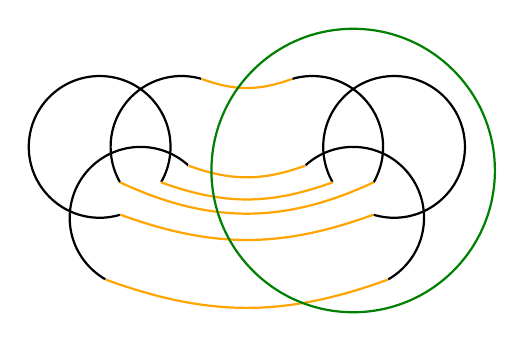
\begin{tikzpicture}[scale=.6]

\coordinate (mid1) at (-90:1);
\coordinate (mid2) at (30:1);
\coordinate (mid3) at (150:1);

\foreach\x in {1,2,3}
{
    % FIXED: Made the path name global and changed format to circL\x
    \draw[thick, name path global=circL\x](mid\x) circle (1.5);
}

\coordinate (e) at (-2.5,0);

\coordinate (1) at ($1.5*(mid1)$);
\coordinate (2) at ($1.5*(mid2)$);
\coordinate (3) at ($1.5*(mid3)$);

\coordinate (12) at ($.9*(mid1) + .9*(mid2)$);
\coordinate (13) at ($.9*(mid1) + .9*(mid3)$);
\coordinate (23) at ($.9*(mid2) + .9*(mid3)$);

\coordinate (123) at (0,0);

% FIXED: Made the mask path global
\filldraw[fill=white, fill opacity=1, draw=white, dashed, name path global=maskL] (3) -- ++(0,2) -- ++(-1.5,0) -- ++(0,-6) -- ++(4,0) -- ++(-1,2) -- (12) -- (123) -- (13) -- cycle;


\begin{scope}[xscale=-1, xshift=4.5cm]
    \coordinate (rmid1) at (-90:1);
    \coordinate (rmid2) at (30:1);
    \coordinate (rmid3) at (150:1);
    
    \foreach\x in {1,2,3}
    {
        % FIXED: Made the path name global and changed format to circR\x
        \draw[thick, name path global=circR\x](rmid\x) circle (1.5);
    }
    
    \coordinate (e) at (-2.5,0);
    
    \coordinate (1) at ($1.5*(rmid1)$);
    \coordinate (2) at ($1.5*(rmid2)$);
    \coordinate (3) at ($1.5*(rmid3)$);
    
    \coordinate (12) at ($.9*(rmid1) + .9*(rmid2)$);
    \coordinate (13) at ($.9*(rmid1) + .9*(rmid3)$);
    \coordinate (23) at ($.9*(rmid2) + .9*(rmid3)$);
    
    \coordinate (123) at (0,0);
    
    % FIXED: Made the mask path global (since it sits inside the \begin{scope} environment)
    \filldraw[fill=white, fill opacity=1, draw=white, dashed, name path global=maskR] (3) -- ++(0,2) -- ++(-1.5,0) -- ++(0,-6) -- ++(4,0) -- ++(-1,2) -- (12) -- (123) -- (13) -- cycle;

\end{scope}

% Calculate all intersections automatically using the new global names
\path [name intersections={of=circR3 and maskR, name=i3R}];
\path [name intersections={of=circR1 and maskR, name=i1R}];
\path [name intersections={of=circR2 and maskR, name=i2R}];

\path [name intersections={of=circL3 and maskL, name=i3L}];
\path [name intersections={of=circL1 and maskL, name=i1L}];
\path [name intersections={of=circL2 and maskL, name=i2L}];

% Map the automatic intersections to your original variable names
\coordinate (A) at (i3R-1);
\coordinate (B) at (i3R-2);
\coordinate (C) at (i1R-1);
\coordinate (D) at (i1R-2);
\coordinate (F) at (i2R-1); 
\coordinate (E) at (i2R-2);

\coordinate (AA) at (i3L-1);
\coordinate (BB) at (i3L-2);
\coordinate (CC) at (i1L-1);
\coordinate (DD) at (i1L-2);
\coordinate (EE) at (i2L-2);
\coordinate (FF) at (i2L-1);

\draw[thick, Orange] (A) to[bend left=-20] (AA);
\draw[thick, Orange] (B) to[bend left=-25] (BB);
\draw[thick, Orange] (C) to[bend left=-20] (CC);
\draw[thick, Orange] (D) to[bend left=-20] (DD);
\draw[thick, Orange] (E) to[bend left=-20] (EE);
\draw[thick, Orange] (F) to[bend left=-20] (FF);

\draw[Green, thick] (0,0) circle (3cm);

\end{tikzpicture}
		\caption{Venn diagram unfolding}
		\label{fig:venn unfolding}
	\end{subfigure}
	\hfill
	% Subfigure 2
	\begin{subfigure}[b]{0.48\textwidth}
		\centering
		
\tikzset{
    triple/.style={
        double,
        double distance=2pt, % Adjust this to change the overall width
        postaction={draw=Orange, line width=0.4pt} % Draws the center line
    }
}

    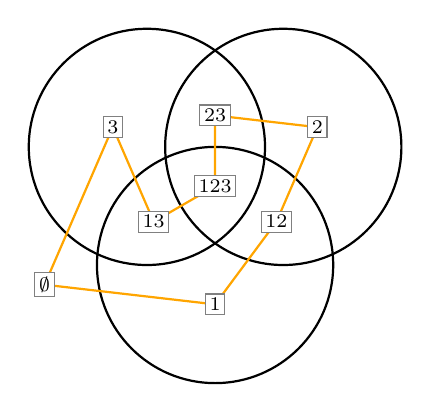
\begin{tikzpicture}



\coordinate (mid1) at (-90:1);
\coordinate (mid2) at (30:1);
\coordinate (mid3) at (150:1);

\foreach\x in {1,2,3}
{
    \draw[thick](mid\x) circle (1.5);
}

\coordinate (e) at ($2.5*(mid1) + 2.5*(mid3)$);

\coordinate (1) at ($1.5*(mid1)$);
\coordinate (2) at ($1.5*(mid2)$);
\coordinate (3) at ($1.5*(mid3)$);

\coordinate (12) at ($.9*(mid1) + .9*(mid2)$);
\coordinate (13) at ($.9*(mid1) + .9*(mid3)$);
\coordinate (23) at ($.9*(mid2) + .9*(mid3)$);

\coordinate (123) at (0,0);


\draw[thick,Orange, thick] (1) 
\foreach\x in {12,2,23,123,13,3,e,1}{ -- (\x)};

\foreach\x in {1,2,3,12,13,23,123}
{
    \node[fill=white, draw=gray , inner sep=1.5pt] at (\x) {\scriptsize\x};
}
\node[fill=white, draw=gray, inner sep=1.5pt] at (e) {\scriptsize$\emptyset$};



    \end{tikzpicture}
		\caption{Venn diagram zigzagging}
		\label{fig:venn zigzagging}
	\end{subfigure}

	\caption{Two constructions for a Venn diagram for the subsets of $\{1,2,3,4\}$. (\textsc{a}) Obtained by unfolding a diagram for $\{1,2,3\}$. The orange lines connect the two parts and the green curve separates regions representing sets which contain 4 from regions that do not. (\textsc{b}) Constructed by inserting a Hamilton cycle of the dual as a new curve.}
	\label{fig:combined_venn}
\end{figure}


In this paper, we extend the study of \defn{rhombic strips} in graded posets. A rhombic strip is a specific crossing-free drawing of a graded poset's diagram on the sphere, where elements of the same rank share a circle of latitude, and the bounded faces are degree-4 rhombi, see \Cref{fig:B4 on sphere} and \Cref{fig:B4 on plane}. Find detailed definitions below.

By analyzing these strips, we can bridge Gray codes and geometry. Their power comes from the fact that they can be constructed using geometric operations. Cut, mirrored and shifted versions of different strips can be stitched together into new strips, as we will see. The corresponding combinatorial objects are then presented on the sphere in a highly structured way, often giving strong results.

\begin{figure}
	\centering
	
    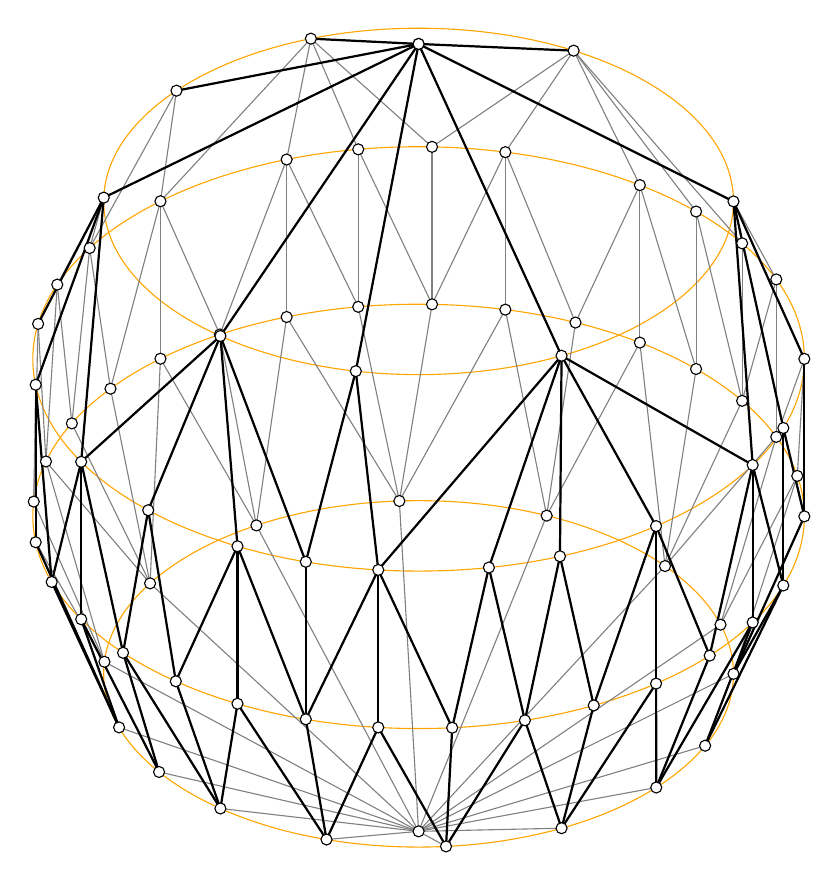
\begin{tikzpicture}[
        x={(1cm, 0cm)},
        y={(0cm, 0.55cm)},
        z={(0cm, 1cm)}
    ]
\foreach\z/\r in {0/4,2/4.9,4/4.9,6/4}{
    \begin{scope}[canvas is xy plane at z=\z]
        \draw[Orange] (0,0) circle[radius=\r];
    \end{scope}
}

\coordinate (empty) at (0,0,-2);
\coordinate (xxxx) at (0,0,8);

\def\anglestep{11}

    \begin{scope}[canvas is xy plane at z=0]
        \coordinate (0000) at (0*\anglestep:4);
        \coordinate (0100) at (1.50*\anglestep:4);
        \coordinate (1100) at (3.50*\anglestep:4);
        \coordinate (1000) at (6.00*\anglestep:4);
        \coordinate (1010) at (8.50*\anglestep:4);
        \coordinate (1110) at (11.00*\anglestep:4);
        \coordinate (1111) at (13.50*\anglestep:4);
        \coordinate (1011) at (16.00*\anglestep:4);
        \coordinate (1001) at (18.00*\anglestep:4);
        \coordinate (1101) at (19.50*\anglestep:4);
        \coordinate (0101) at (21.00*\anglestep:4);
        \coordinate (0001) at (23.00*\anglestep:4);
        \coordinate (0011) at (25.00*\anglestep:4);
        \coordinate (0111) at (27.00*\anglestep:4);
        \coordinate (0110) at (29.00*\anglestep:4);
        \coordinate (0010) at (30.50*\anglestep:4);
    \end{scope}

\begin{scope}[canvas is xy plane at z=2]
    \coordinate (x000) at (0*\anglestep:4.9);
    \coordinate (0x00) at (1*\anglestep:4.9);
    \coordinate (x100) at (2*\anglestep:4.9);
    \coordinate (11x0) at (3*\anglestep:4.9);
    \coordinate (110x) at (4*\anglestep:4.9);
    \coordinate (1x00) at (5*\anglestep:4.9);
    \coordinate (100x) at (6*\anglestep:4.9);
    \coordinate (10x0) at (7*\anglestep:4.9);
    \coordinate (101x) at (8*\anglestep:4.9);
    \coordinate (x010) at (9*\anglestep:4.9);
    \coordinate (1x10) at (10*\anglestep:4.9);
    \coordinate (x110) at (11*\anglestep:4.9);
    \coordinate (111x) at (12*\anglestep:4.9);
    \coordinate (x111) at (13*\anglestep:4.9);
    \coordinate (11x1) at (14*\anglestep:4.9);
    \coordinate (1x11) at (15*\anglestep:4.9);
    \coordinate (x011) at (16*\anglestep:4.9);
    \coordinate (10x1) at (17*\anglestep:4.9);
    \coordinate (x001) at (18*\anglestep:4.9);
    \coordinate (1x01) at (19*\anglestep:4.9);
    \coordinate (x101) at (20*\anglestep:4.9);
    \coordinate (010x) at (21*\anglestep:4.9);
    \coordinate (0x01) at (22*\anglestep:4.9);
    \coordinate (000x) at (23*\anglestep:4.9);
    \coordinate (00x1) at (24*\anglestep:4.9);
    \coordinate (001x) at (25*\anglestep:4.9);
    \coordinate (0x11) at (26*\anglestep:4.9);
    \coordinate (01x1) at (27*\anglestep:4.9);
    \coordinate (011x) at (28*\anglestep:4.9);
    \coordinate (01x0) at (29*\anglestep:4.9);
    \coordinate (0x10) at (30*\anglestep:4.9);
    \coordinate (00x0) at (31*\anglestep:4.9);
\end{scope}

\begin{scope}[canvas is xy plane at z=4]
    \coordinate (xx00) at (0*\anglestep:4.9);
    \coordinate (x1x0) at (2*\anglestep:4.9);
    \coordinate (1xx0) at (3.0*\anglestep:4.9);
    \coordinate (11xx) at (4*\anglestep:4.9);
    \coordinate (1x0x) at (5.0*\anglestep:4.9);
    \coordinate (10xx) at (7.0*\anglestep:4.9);
    \coordinate (1x1x) at (8.0*\anglestep:4.9);
    \coordinate (x01x) at (9*\anglestep:4.9);
    \coordinate (xx10) at (10.0*\anglestep:4.9);
    \coordinate (x11x) at (12.0*\anglestep:4.9);
    \coordinate (x1x1) at (13.5*\anglestep:4.9);
    \coordinate (1xx1) at (14.5*\anglestep:4.9);
    \coordinate (xx11) at (15.5*\anglestep:4.9);
    \coordinate (x0x1) at (17.0*\anglestep:4.9);
    \coordinate (xx01) at (19.0*\anglestep:4.9);
    \coordinate (x10x) at (20.5*\anglestep:4.9);
    \coordinate (0x0x) at (22.0*\anglestep:4.9);
    \coordinate (x00x) at (23.0*\anglestep:4.9);
    \coordinate (00xx) at (24.0*\anglestep:4.9);
    \coordinate (0x1x) at (25.5*\anglestep:4.9);
    \coordinate (0xx1) at (26.5*\anglestep:4.9);
    \coordinate (01xx) at (28.0*\anglestep:4.9);
    \coordinate (0xx0) at (30.0*\anglestep:4.9);
    \coordinate (x0x0) at (31*\anglestep:4.9);
    \coordinate (xx00e) at (32*\anglestep:4.9);
\end{scope}

\begin{scope}[canvas is xy plane at z=6]
    \coordinate (xxx0) at (0*\anglestep:4);
    \coordinate (1xxx) at (5.5*\anglestep:4);
    \coordinate (xx1x) at (10.0*\anglestep:4);
    \coordinate (x1xx) at (12.75*\anglestep:4);
    \coordinate (xxx1) at (16.25*\anglestep:4);
    \coordinate (xx0x) at (21.0*\anglestep:4);
    \coordinate (x0xx) at (23.5*\anglestep:4);
    \coordinate (0xxx) at (27.0*\anglestep:4);
\end{scope}




\foreach \a/\b in {x000/xx00, xx00/xxx0, 0000/0x00, 0x00/xx00, x100/xx00, x1x0/xxx0, 1xx0/xxx0, 1110/1x10, 1011/x011, 01x0/0xx0, 1001/10x1, 000x/0x0x, 00xx/0xxx, 0111/0x11, 101x/x01x, x010/xx10, 1000/1x00, 0011/00x1, 0011/001x, x00x/xx0x, 0x1x/0xxx, 1010/10x0, 1xx0/1xxx, 1xx1/xxx1, x001/x0x1, 00x0/x0x0, x010/x01x, 001x/0x1x, 110x/11xx, 1101/1x01, 1110/x110, 101x/10xx, 11x0/x1x0, 0x10/0xx0, 1001/1x01, 0101/010x, x101/xx01, x101/x10x, x001/xx01, 0001/000x, 00xx/x0xx, 101x/1x1x, x10x/xx0x, x11x/x1xx, x1x1/xxx1, 001x/00xx, 000x/00xx, 0110/0x10, 1x11/xx11, 1110/111x, xx10/xx1x, 1000/100x, 0xx0/0xxx, x01x/xx1x, 0001/0x01, 011x/01xx, 1111/x111, 010x/0x0x, 1000/10x0, 0101/0x01, x111/x11x, 0111/011x, 1100/x100, 110x/1x0x, 00x1/00xx, 1101/x101, 01x1/01xx, 11x1/x1x1, 11x0/1xx0, x011/xx11, 111x/x11x, x11x/xx1x, x011/x0x1, x0x1/xxx1, 0x11/0x1x, 01xx/0xxx, 1111/111x, xx01/xx0x, 10xx/1xxx, 1010/101x, 0000/x000, 0x0x/xx0x, 0001/00x1, 010x/x10x, 0010/00x0, 100x/1x0x, 0111/01x1, xx11/xxx1, xx01/xxx1, 1011/10x1, 00x0/0xx0, 1x1x/xx1x, 01x1/0xx1, 1x1x/1xxx, 0xx1/0xxx, x110/xx10, 1010/1x10, 1x10/xx10, 11x1/1xx1, 1x11/1xx1, 1111/1x11, 11x0/11xx, 10x0/10xx, 0101/x101, 1x01/xx01, 1100/1x00, 0011/0x11, 1001/x001, 0110/011x, 11xx/1xxx, 1x0x/1xxx, 0100/0x00, 0x11/0xx1, 0x01/0x0x, 0010/0x10, 1011/1x11, 100x/10xx, x00x/x0xx, 10x1/x0x1, 1100/110x, x100/x1x0, 1010/x010, 000x/x00x, x110/x11x, x111/x1x1, 0110/01x0, 1x00/1x0x, 1111/11x1, 1100/11x0, x1x1/x1xx, 01x0/01xx, 0100/x100, 0000/00x0, 0000/x000, x000/xx00, xx00/xxx0, 0xx0/xxx0, x0x0/xxx0,x000/x0x0,xxx0/xxxx,xx0x/xxxx,x0xx/xxxx,0xxx/xxxx,xxx1/xxxx,xx1x/xxxx,x1xx/xxxx,1xxx/xxxx}
{  \draw[thin, gray] (\a) -- (\b);  }
\foreach\a in {0,1}{
    \foreach\b in {0,1}{
        \foreach\c in {0,1}{
            \foreach\d in {0,1}{
                \draw[thin, gray] (empty) -- (\a\b\c\d);
            }
        }
    }
}

\foreach\a/\b in {x000/xx00, xx00/xxx0, 01x0/0xx0, 1001/10x1, 000x/0x0x, 00xx/0xxx, 0111/0x11,
    0011/00x1, 0011/001x, x00x/xx0x, 0x1x/0xxx, x001/x0x1, 00x0/x0x0, 001x/0x1x,
    1101/1x01, 0x10/0xx0, 1001/1x01, 0101/010x, x101/xx01, x101/x10x, x001/xx01,
    0001/000x, 00xx/x0xx, x10x/xx0x, 001x/00xx, 000x/00xx, 0110/0x10, 0xx0/0xxx,
    0001/0x01, 011x/01xx, 010x/0x0x, 0101/0x01, 0111/011x, 00x1/00xx, 1101/x101,
    01x1/01xx, 0x11/0x1x, 01xx/0xxx, xx01/xx0x, 0000/x000, 0x0x/xx0x, 0001/00x1,
    010x/x10x, 0010/00x0, 0111/01x1, 00x0/0xx0, 01x1/0xx1, 0xx1/0xxx, 0101/x101,
    1x01/xx01, 0011/0x11, 1001/x001, 0110/011x, 0x11/0xx1, 0x01/0x0x, 0010/0x10,
    x00x/x0xx, 10x1/x0x1, 000x/x00x, 0110/01x0, 01x0/01xx, 0000/00x0, 0xx0/xxx0,
    x0x0/xxx0, x000/x0x0,xxx0/xxxx,xx0x/xxxx,x0xx/xxxx,0xxx/xxxx,xxx1/xxxx,xx1x/xxxx,x1xx/xxxx,1xxx/xxxx,xxx1/xx11,xxx1/x0x1,xxx1/xx01}
    {\draw[thick] (\a) -- (\b);}

\foreach\a in {0,1,x}{
    \foreach\b in {0,1,x}{
        \foreach\c in {0,1,x}{
            \foreach\d in {0,1,x}{
                \filldraw[fill=white] (\a\b\c\d) circle (2pt);
                %\node[fill=white, draw, inner sep=1pt] at (\a\b\c\d) {\tiny \a\b\c\d};
            }
        }
    }
}
\filldraw[fill=white] (empty) circle (2pt);
\filldraw[fill=white] (xxxx) circle (2pt);
        
    \end{tikzpicture}
	\caption{A cyclic rhombic strip of the face lattice of the 4-dimensional cube. Vertex labels are omitted for visibility. Circles of latitude are drawn in orange to indicate the ranks.}
	\label{fig:B4 on sphere}
\end{figure}

\begin{figure}
	\centering
	\makebox[\textwidth][c]{
		\newcommand{\clrone}{blue}
\newcommand{\clrtwo}{red}

% Custom macro to create a tightly spaced 2x2 grid
\newcommand{\fg}[4]{%
  \renewcommand{\arraystretch}{0.6}%
  \setlength{\tabcolsep}{0.7pt}%
  \begin{tabular}{@{}cc@{}}#1 & #2 \\[-0.0ex] #3 & #4\end{tabular}%
}

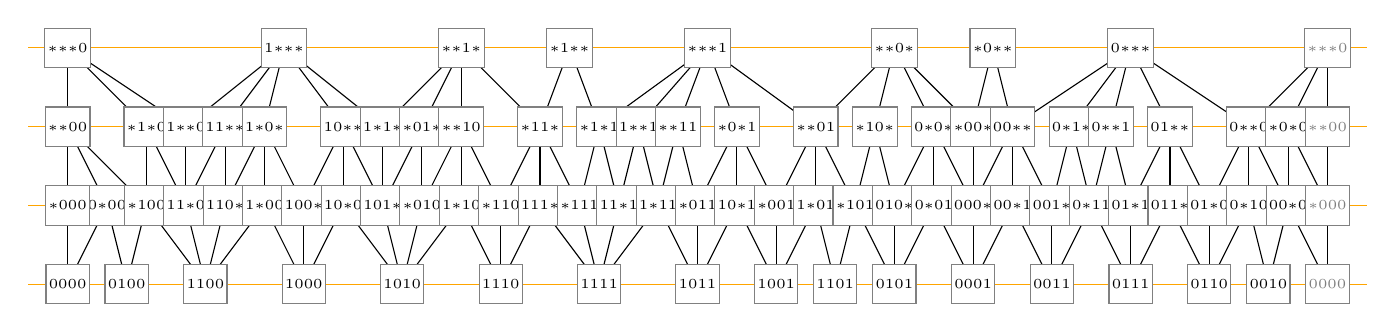
\begin{tikzpicture}[every node/.style={font=\tiny, inner sep=1pt, gray, text=black, minimum size=5mm},scale=0.5]
\coordinate (0000) at (0, 0);
\coordinate (0100) at (1.5, 0);
\coordinate (1100) at (3.5, 0);
\coordinate (1000) at (6.0, 0);
\coordinate (1010) at (8.5, 0);
\coordinate (1110) at (11.0, 0);
\coordinate (1111) at (13.5, 0);
\coordinate (1011) at (16.0, 0);
\coordinate (1001) at (18.0, 0);
\coordinate (1101) at (19.5, 0);
\coordinate (0101) at (21.0, 0);
\coordinate (0001) at (23.0, 0);
\coordinate (0011) at (25.0, 0);
\coordinate (0111) at (27.0, 0);
\coordinate (0110) at (29.0, 0);
\coordinate (0010) at (30.5, 0);
\coordinate (0000e) at (32, 0);

\coordinate (x000) at (0, 2);
\coordinate (0x00) at (1, 2);
\coordinate (x100) at (2, 2);
\coordinate (11x0) at (3, 2);
\coordinate (110x) at (4, 2);
\coordinate (1x00) at (5, 2);
\coordinate (100x) at (6, 2);
\coordinate (10x0) at (7, 2);
\coordinate (101x) at (8, 2);
\coordinate (x010) at (9, 2);
\coordinate (1x10) at (10, 2);
\coordinate (x110) at (11, 2);
\coordinate (111x) at (12, 2);
\coordinate (x111) at (13, 2);
\coordinate (11x1) at (14, 2);
\coordinate (1x11) at (15, 2);
\coordinate (x011) at (16, 2);
\coordinate (10x1) at (17, 2);
\coordinate (x001) at (18, 2);
\coordinate (1x01) at (19, 2);
\coordinate (x101) at (20, 2);
\coordinate (010x) at (21, 2);
\coordinate (0x01) at (22, 2);
\coordinate (000x) at (23, 2);
\coordinate (00x1) at (24, 2);
\coordinate (001x) at (25, 2);
\coordinate (0x11) at (26, 2);
\coordinate (01x1) at (27, 2);
\coordinate (011x) at (28, 2);
\coordinate (01x0) at (29, 2);
\coordinate (0x10) at (30, 2);
\coordinate (00x0) at (31, 2);
\coordinate (x000e) at (32, 2);

\coordinate (xx00) at (0, 4);
\coordinate (x1x0) at (2, 4);
\coordinate (1xx0) at (3.0, 4);
\coordinate (11xx) at (4, 4);
\coordinate (1x0x) at (5.0, 4);
\coordinate (10xx) at (7.0, 4);
\coordinate (1x1x) at (8.0, 4);
\coordinate (x01x) at (9, 4);
\coordinate (xx10) at (10.0, 4);
\coordinate (x11x) at (12.0, 4);
\coordinate (x1x1) at (13.5, 4);
\coordinate (1xx1) at (14.5, 4);
\coordinate (xx11) at (15.5, 4);
\coordinate (x0x1) at (17.0, 4);
\coordinate (xx01) at (19.0, 4);
\coordinate (x10x) at (20.5, 4);
\coordinate (0x0x) at (22.0, 4);
\coordinate (x00x) at (23.0, 4);
\coordinate (00xx) at (24.0, 4);
\coordinate (0x1x) at (25.5, 4);
\coordinate (0xx1) at (26.5, 4);
\coordinate (01xx) at (28.0, 4);
\coordinate (0xx0) at (30.0, 4);
\coordinate (x0x0) at (31, 4);
\coordinate (xx00e) at (32, 4);

\coordinate (xxx0) at (0, 6);
\coordinate (1xxx) at (5.5, 6);
\coordinate (xx1x) at (10.0, 6);
\coordinate (x1xx) at (12.75, 6);
\coordinate (xxx1) at (16.25, 6);
\coordinate (xx0x) at (21.0, 6);
\coordinate (x0xx) at (23.5, 6);
\coordinate (0xxx) at (27.0, 6);
\coordinate (xxx0e) at (32, 6);


\foreach \a/\b in {x000/xx00, xx00/xxx0, 0000/0x00, 0x00/xx00, x100/xx00, x1x0/xxx0, 1xx0/xxx0, 1110/1x10, 1011/x011, 01x0/0xx0, 1001/10x1, 000x/0x0x, 00xx/0xxx, 0111/0x11, 101x/x01x, x010/xx10, 1000/1x00, 0011/00x1, 0011/001x, x00x/xx0x, 0x1x/0xxx, 1010/10x0, 1xx0/1xxx, 1xx1/xxx1, x001/x0x1, 00x0/x0x0, x010/x01x, 001x/0x1x, 110x/11xx, 1101/1x01, 1110/x110, 101x/10xx, 11x0/x1x0, 0x10/0xx0, 1001/1x01, 0101/010x, x101/xx01, x101/x10x, x001/xx01, 0001/000x, 00xx/x0xx, 101x/1x1x, x10x/xx0x, x11x/x1xx, x1x1/xxx1, 001x/00xx, 000x/00xx, 0110/0x10, 1x11/xx11, 1110/111x, xx10/xx1x, 1000/100x, 0xx0/0xxx, x01x/xx1x, 0001/0x01, 011x/01xx, 1111/x111, 010x/0x0x, 1000/10x0, 0101/0x01, x111/x11x, 0111/011x, 1100/x100, 110x/1x0x, 00x1/00xx, 1101/x101, 01x1/01xx, 11x1/x1x1, 11x0/1xx0, x011/xx11, 111x/x11x, x11x/xx1x, x011/x0x1, x0x1/xxx1, 0x11/0x1x, 01xx/0xxx, 1111/111x, xx01/xx0x, 10xx/1xxx, 1010/101x, 0000/x000, 0x0x/xx0x, 0001/00x1, 010x/x10x, 0010/00x0, 100x/1x0x, 0111/01x1, xx11/xxx1, xx01/xxx1, 1011/10x1, 00x0/0xx0, 1x1x/xx1x, 01x1/0xx1, 1x1x/1xxx, 0xx1/0xxx, x110/xx10, 1010/1x10, 1x10/xx10, 11x1/1xx1, 1x11/1xx1, 1111/1x11, 11x0/11xx, 10x0/10xx, 0101/x101, 1x01/xx01, 1100/1x00, 0011/0x11, 1001/x001, 0110/011x, 11xx/1xxx, 1x0x/1xxx, 0100/0x00, 0x11/0xx1, 0x01/0x0x, 0010/0x10, 1011/1x11, 100x/10xx, x00x/x0xx, 10x1/x0x1, 1100/110x, x100/x1x0, 1010/x010, 000x/x00x, x110/x11x, x111/x1x1, 0110/01x0, 1x00/1x0x, 1111/11x1, 1100/11x0, x1x1/x1xx, 01x0/01xx, 0100/x100, 0000e/00x0, 0000e/x000e, x000e/xx00e, xx00e/xxx0e, 0xx0/xxx0e, x0x0/xxx0e,x000e/x0x0}
{  \draw (\a) -- (\b);  }

\foreach\y in {0,2,4,6}{
    \draw[thin,Orange] (-1,\y) -- (33,\y);
}

\node[draw, fill = white] at (0000) {\fg{0}{0}{0}{0}};
\node[draw, fill = white] at (0100) {\fg{0}{1}{0}{0}};
\node[draw, fill = white] at (1100) {\fg{1}{1}{0}{0}};
\node[draw, fill = white] at (1000) {\fg{1}{0}{0}{0}};
\node[draw, fill = white] at (1010) {\fg{1}{0}{1}{0}};
\node[draw, fill = white] at (1110) {\fg{1}{1}{1}{0}};
\node[draw, fill = white] at (1111) {\fg{1}{1}{1}{1}};
\node[draw, fill = white] at (1011) {\fg{1}{0}{1}{1}};
\node[draw, fill = white] at (1001) {\fg{1}{0}{0}{1}};
\node[draw, fill = white] at (1101) {\fg{1}{1}{0}{1}};
\node[draw, fill = white] at (0101) {\fg{0}{1}{0}{1}};
\node[draw, fill = white] at (0001) {\fg{0}{0}{0}{1}};
\node[draw, fill = white] at (0011) {\fg{0}{0}{1}{1}};
\node[draw, fill = white] at (0111) {\fg{0}{1}{1}{1}};
\node[draw, fill = white] at (0110) {\fg{0}{1}{1}{0}};
\node[draw, fill = white] at (0010) {\fg{0}{0}{1}{0}};
\node[draw, fill = white] at (0000) {\fg{0}{0}{0}{0}};
\node[fill = white] at (0000e) {};
\node[draw=gray, fill = white,minimum size=5mm] at (0000e) {\textcolor{gray}{\fg{0}{0}{0}{0}}};

\node[draw, fill = white] at (x000) {\fg{$*$}{0}{0}{0}};
\node[draw, fill = white] at (0x00) {\fg{0}{$*$}{0}{0}};
\node[draw, fill = white] at (x100) {\fg{$*$}{1}{0}{0}};
\node[draw, fill = white] at (11x0) {\fg{1}{1}{$*$}{0}};
\node[draw, fill = white] at (110x) {\fg{1}{1}{0}{$*$}};
\node[draw, fill = white] at (1x00) {\fg{1}{$*$}{0}{0}};
\node[draw, fill = white] at (100x) {\fg{1}{0}{0}{$*$}};
\node[draw, fill = white] at (10x0) {\fg{1}{0}{$*$}{0}};
\node[draw, fill = white] at (101x) {\fg{1}{0}{1}{$*$}};
\node[draw, fill = white] at (x010) {\fg{$*$}{0}{1}{0}};
\node[draw, fill = white] at (1x10) {\fg{1}{$*$}{1}{0}};
\node[draw, fill = white] at (x110) {\fg{$*$}{1}{1}{0}};
\node[draw, fill = white] at (111x) {\fg{1}{1}{1}{$*$}};
\node[draw, fill = white] at (x111) {\fg{$*$}{1}{1}{1}};
\node[draw, fill = white] at (11x1) {\fg{1}{1}{$*$}{1}};
\node[draw, fill = white] at (1x11) {\fg{1}{$*$}{1}{1}};
\node[draw, fill = white] at (x011) {\fg{$*$}{0}{1}{1}};
\node[draw, fill = white] at (10x1) {\fg{1}{0}{$*$}{1}};
\node[draw, fill = white] at (x001) {\fg{$*$}{0}{0}{1}};
\node[draw, fill = white] at (1x01) {\fg{1}{$*$}{0}{1}};
\node[draw, fill = white] at (x101) {\fg{$*$}{1}{0}{1}};
\node[draw, fill = white] at (010x) {\fg{0}{1}{0}{$*$}};
\node[draw, fill = white] at (0x01) {\fg{0}{$*$}{0}{1}};
\node[draw, fill = white] at (000x) {\fg{0}{0}{0}{$*$}};
\node[draw, fill = white] at (00x1) {\fg{0}{0}{$*$}{1}};
\node[draw, fill = white] at (001x) {\fg{0}{0}{1}{$*$}};
\node[draw, fill = white] at (0x11) {\fg{0}{$*$}{1}{1}};
\node[draw, fill = white] at (01x1) {\fg{0}{1}{$*$}{1}};
\node[draw, fill = white] at (011x) {\fg{0}{1}{1}{$*$}};
\node[draw, fill = white] at (01x0) {\fg{0}{1}{$*$}{0}};
\node[draw, fill = white] at (0x10) {\fg{0}{$*$}{1}{0}};
\node[draw, fill = white] at (00x0) {\fg{0}{0}{$*$}{0}};
\node[draw, fill = white] at (x000) {\fg{$*$}{0}{0}{0}};
\node[fill = white] at (x000e) {};
\node[draw=gray, fill = white,minimum size=5mm] at (x000e) {\textcolor{gray}{\fg{$*$}{0}{0}{0}}};

\node[draw, fill = white] at (xx00) {\fg{$*$}{$*$}{0}{0}};
\node[draw, fill = white] at (x1x0) {\fg{$*$}{1}{$*$}{0}};
\node[draw, fill = white] at (1xx0) {\fg{1}{$*$}{$*$}{0}};
\node[draw, fill = white] at (11xx) {\fg{1}{1}{$*$}{$*$}};
\node[draw, fill = white] at (1x0x) {\fg{1}{$*$}{0}{$*$}};
\node[draw, fill = white] at (10xx) {\fg{1}{0}{$*$}{$*$}};
\node[draw, fill = white] at (1x1x) {\fg{1}{$*$}{1}{$*$}};
\node[draw, fill = white] at (x01x) {\fg{$*$}{0}{1}{$*$}};
\node[draw, fill = white] at (xx10) {\fg{$*$}{$*$}{1}{0}};
\node[draw, fill = white] at (x11x) {\fg{$*$}{1}{1}{$*$}};
\node[draw, fill = white] at (x1x1) {\fg{$*$}{1}{$*$}{1}};
\node[draw, fill = white] at (1xx1) {\fg{1}{$*$}{$*$}{1}};
\node[draw, fill = white] at (xx11) {\fg{$*$}{$*$}{1}{1}};
\node[draw, fill = white] at (x0x1) {\fg{$*$}{0}{$*$}{1}};
\node[draw, fill = white] at (xx01) {\fg{$*$}{$*$}{0}{1}};
\node[draw, fill = white] at (x10x) {\fg{$*$}{1}{0}{$*$}};
\node[draw, fill = white] at (0x0x) {\fg{0}{$*$}{0}{$*$}};
\node[draw, fill = white] at (x00x) {\fg{$*$}{0}{0}{$*$}};
\node[draw, fill = white] at (00xx) {\fg{0}{0}{$*$}{$*$}};
\node[draw, fill = white] at (0x1x) {\fg{0}{$*$}{1}{$*$}};
\node[draw, fill = white] at (0xx1) {\fg{0}{$*$}{$*$}{1}};
\node[draw, fill = white] at (01xx) {\fg{0}{1}{$*$}{$*$}};
\node[draw, fill = white] at (0xx0) {\fg{0}{$*$}{$*$}{0}};
\node[draw, fill = white] at (x0x0) {\fg{$*$}{0}{$*$}{0}};
\node[draw, fill = white] at (xx00) {\fg{$*$}{$*$}{0}{0}};
\node[fill = white] at (xx00e) {};
\node[draw=gray, fill = white,minimum size=5mm] at (xx00e) {\textcolor{gray}{\fg{$*$}{$*$}{0}{0}}};

\node[draw, fill = white] at (xxx0) {\fg{$*$}{$*$}{$*$}{0}};
\node[draw, fill = white] at (1xxx) {\fg{1}{$*$}{$*$}{$*$}};
\node[draw, fill = white] at (xx1x) {\fg{$*$}{$*$}{1}{$*$}};
\node[draw, fill = white] at (x1xx) {\fg{$*$}{1}{$*$}{$*$}};
\node[draw, fill = white] at (xxx1) {\fg{$*$}{$*$}{$*$}{1}};
\node[draw, fill = white] at (xx0x) {\fg{$*$}{$*$}{0}{$*$}};
\node[draw, fill = white] at (x0xx) {\fg{$*$}{0}{$*$}{$*$}};
\node[draw, fill = white] at (0xxx) {\fg{0}{$*$}{$*$}{$*$}};
\node[draw, fill = white] at (xxx0) {\fg{$*$}{$*$}{$*$}{0}};
\node[fill = white] at (xxx0e) {};
\node[draw=gray, fill = white,minimum size=5mm] at (xxx0e) {\textcolor{gray}{\fg{$*$}{$*$}{$*$}{0}}};

\end{tikzpicture}
	}
	\caption{The cyclic rhombic strip of the face lattice of the 4-dimensional cube from \Cref{fig:B4 on sphere} on the plane. Note that the leftmost and rightmost chains are equal and that empty set and full cube have been omitted in this version. The ranks are indicated by orange lines as in \Cref{fig:B4 on sphere}.}
	\label{fig:B4 on plane}
\end{figure}

A rhombic strip $R$ of a graded poset $P$ defines orderings of the ranks of $P$. Because two adjacent elements on a circle of latitude are connected to a common element one rank below and one rank above, they are related to each other by a pair of cover relations of $P$ in two different ways. This means that these elements are minimally different, and hence the rhombic strip induces Gray codes for the ranks of $P$. For example, the $k$'th rank of the Boolean lattice of subsets is given by subsets of $[n]$ which contain $k$ elements, also known as $k$-combinations. The cover relations of the Boolean lattice consist of single element removals (or insertions). Hence, a rhombic strip of the Boolean lattice induces a Gray code of $k$-combinations such that adjacent subsets have a symmetric difference of size 2, for any $0\le k\le n$. As claimed above, we can realize the BRGC as a Hamilton cycle of such a rhombic strip, and we will obtain the additional property that this Hamilton cycle visits the elements of a rank in the order they appear in the strip. This proves that the BRGC restricts to a Gray code of $k$-combinations of $[n]$, for any $0\le k\le n$. Similarly, we obtain that the SJT Gray code restricts to a Gray code for permutations with a fixed number $k$ of inversions. This reproves a result of Vajnovszki and Vernay~\cite{restrictedinversions}.

It is also common for $P$ to be the face lattice of a polytope $\mathcal P$. In this case, the elements of rank $k+1$ are the faces of dimension $k$. Rank $k+1$ of a rhombic strip is then a listing of the $k$-dimensional faces such that the intersection and the span of two adjacent faces are $k-1$ and $k+1$ dimensional, respectively. For extremal $k$, such listings consist of Hamilton paths or cycles of $\mathcal P$ and its dual.

The paper is structured as follows: We give the formal statements of our results in \Cref{sec:results}. After that, in \Cref{sec:prelim}, we give detailed definitions and define notation. \Cref{sec:related} puts the results in a context of related work. In \Cref{sec:proofs}, we give the proofs, and in \Cref{sec:conclusion} we review the findings and state open problems.

\begin{figure}
	\centering
	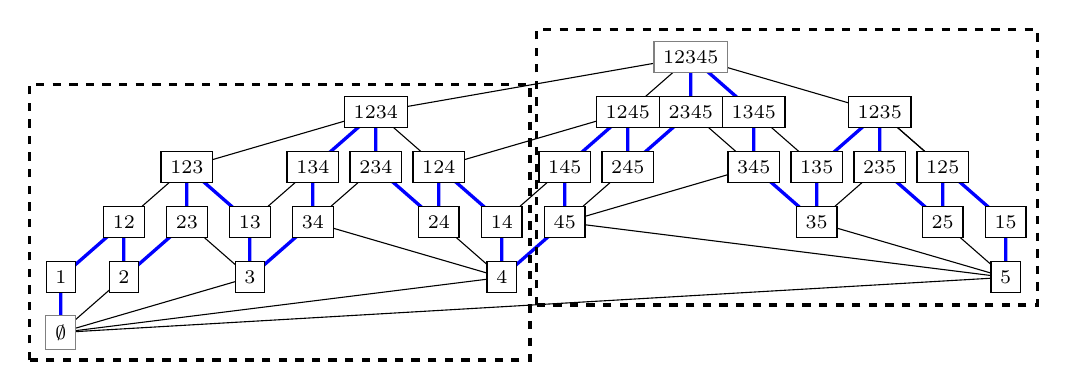
\begin{tikzpicture}[yscale = 0.35, xscale=0.4, every node/.style={font=\scriptsize}]
\coordinate (12) at (2,2);
\coordinate (23) at (4,2);
\coordinate (13) at (6,2);
\coordinate (34) at (8,2);
\coordinate (24) at (12,2);
\coordinate (14) at (14,2);
\coordinate (45) at (16,2);
\coordinate (35) at (24,2);
\coordinate (25) at (28,2);
\coordinate (15) at (30,2);

\coordinate (1) at (0,0);
\coordinate (2) at (2,0);
\coordinate (3) at (6,0);
\coordinate (4) at (14,0);
\coordinate (5) at (30,0);

\coordinate (123) at (4,4);
\coordinate (134) at (8,4);
\coordinate (234) at (10,4);
\coordinate (124) at (12,4);
\coordinate (145) at (16,4);
\coordinate (245) at (18,4);
\coordinate (345) at (22,4);
\coordinate (135) at (24,4);
\coordinate (235) at (26,4);
\coordinate (125) at (28,4);

\coordinate (1234) at (10,6);
\coordinate (1245) at (18,6);
\coordinate (2345) at (20,6);
\coordinate (1345) at (22,6);
\coordinate (1235) at (26,6);

\coordinate (12345) at (20,8);
\coordinate (e) at (0,-2);

\foreach \a/\b in {1/12,2/12,2/23,3/23,3/13,3/34,4/34,4/24,4/14,4/45,5/45,5/35,5/25,5/15,12/123,23/123,13/123,13/134,34/134,34/234,24/234,24/124,14/124,45/145,45/245,45/345,35/345,35/135,35/235,25/125,15/125,123/1234,134/1234,234/1234,124/1234,124/1245,145/1245,245/1245,245/2345,345/2345,345/1345,135/1345,135/1235,235/1235,125/1235, 14/145,125/1235,25/235, 12345/1234, 12345/1235, 12345/1245, 12345/1345, 12345/2345, e/1,e/2,e/3,e/4,e/5}
{  \draw (\a) -- (\b);  }

\draw[Blue, very thick] (e) -- (1) -- (12) -- (2) -- (23) -- (123) -- (13) -- (3) -- (34) -- (134) -- (1234) -- (234) -- (24) -- (124) -- (14) -- (4) -- (45) -- (145) -- (1245) -- (245) -- (2345) -- (12345) -- (1345) -- (345) -- (35) -- (135) -- (1235) -- (235) -- (25) -- (125) -- (15) -- (5);

\foreach\n in {1,2,3,4,5,12,13,14,15,23,24,25,34,35,45,123,124,125,134,135,145,234,235,245,345,1234,1235,1345,1245,2345}
{ \node[draw, fill = white] at (\n) {$\n$}; }

\node[draw=gray, fill=white] at (12345) {$12345$};
\node[draw=gray, fill=white] at (e) {$\emptyset$};

\draw[very thick, dashed] (-1,-3) -- (-1,7) -- (14.9,7) -- (14.9,-3) -- cycle;

\draw[very thick, dashed] (15.1,-1) -- (15.1,9) -- (31,9) -- (31,-1) -- cycle;

\end{tikzpicture}
	\caption{A rhombic strip for the Boolean lattice for $n=5$. The BRGC is marked in blue. This rhombic strip can be obtained by using the unfolding construction from below. The two parts are marked by dashed boxes. Note that the boxes contain rhombic strips for the Boolean lattice for $n=4$, but once with and once without 5 in every set.}
	\label{fig:boolean with brgc}
\end{figure}

\section{Results}\label{sec:results}

We will first consider the unfolding and zigzagging constructions.

\begin{restatable}[Unfolding]{theorem}{unfolding}\label{thm:unfolding}
	Let $P$ be a graded poset with 0 and 1 such that $P$ admits a (Hamiltonian) non-cyclic rhombic strip and let $b\in\N$ be given. Then $P\times C_b$ admits a (Hamiltonian) rhombic strip. Furthermore, if the left and right boundaries of the given strip meet only at 0 and 1, then $P\times C_{1}$ admits a (Hamiltonian) cyclic rhombic strip.
\end{restatable}

\begin{restatable}[Zigzagging]{theorem}{zigzagging}\label{thm:zigzagging}
	Let $P$ be a graded poset with 0 and 1 such that $P$ admits a (cyclic) Hamiltonian rhombic strip and let $b\in\N$ be given. Then $P\times C_b$ admits a (cyclic) Hamiltonian rhombic strip.
\end{restatable}

Using these, we can prove our first main result. The $k$-combinations of a multiset admit cyclic Gray codes if at least one element of the multiset appears an odd number of times. This follows from the constructions above because the $k$-combinations appear as rank $k$ in a product of chains:

\begin{restatable}[Multiset Combinations]{corollary}{multisetcombinationsRS}\label{thm:multiset combinations}
	If $P=C_{b_1}\times\ldots\times C_{b_n}$ is a product of $n$ chains with $n\ge 3$ and at least one $b_i$ odd, then $P$ admits a cyclic Hamiltonian
	rhombic strip.
\end{restatable}

Adapting the zigzagging construction for this specific problem, we are able to fill the gap and prove the full conjecture of Ruskey and Savage about multiset combinations.
\begin{restatable}[Multiset Combinations]{theorem}{multisetcombinationsfull}\label{thm:multisetcombinationsfull}
	Let $b_1,\ldots,b_n\in\N$, $n\ge 3$, and $0\le k\le b_1+\ldots+b_n$. Then the $k$-combinations of the multiset $\{1^{(b_1)},\ldots,n^{(b_n)}\}$ admit a cyclic Gray code under single replacements.
\end{restatable}

\begin{restatable}[Weak Bruhat Order (\cite{restrictedinversions})]{corollary}{weakBruhat}\label{thm:bruhat}
	For any given $k$, the SJT Gray code for permutations of $[n]$ restricts to Gray codes on the set of permutations with exactly $k$ inversions such that adjacent permutations differ in two adjacent transpositions.
\end{restatable}

Effler and Ruskey~\cite{fixedinversions} give an efficient algorithm for listing permutations with a fixed number of inversions. Here, we recover a Gray code obtained by restricting the SJT ordering.

	We combine the two constructions to obtain a vastly more powerful tool:

\begin{restatable}[Cartesian Products]{theorem}{products}\label{thm:products}
	Let $P$ and $Q$ be graded posets with 0 and 1. Assume that $Q$ admits a non-cyclic rhombic strip and $P$ admits a (cyclic) Hamiltonian rhombic strip. Then $P\times Q$ admits a (cyclic) rhombic strip. If the rhombic strip of $Q$ is Hamiltonian, then $P\times Q$ admits a (cyclic) Hamiltonian rhombic strip.
\end{restatable}
\begin{remark}\label{rem:product-boundaries}
	The strip of $Q$ must be non-cyclic because the construction connects copies along their left and right boundaries. A cyclic strip need not contain a non-cyclic strip, as the examples in \Cref{sec:unsplittable} show, so this case is not covered by the product construction.
\end{remark}
Note that $P=C_b$ yields the unfolding construction and $Q=C_b$ yields zigzagging. The additional cyclic conclusion of \Cref{thm:unfolding} uses a separate closing step.

This tool allows us to prove some strong theorems. First, we obtain rhombic strips for distributive lattices of tree posets. This follows from the theorem above because the non-empty rooted subtrees form a product of the corresponding lattices of the principal subtrees at $r$:

\begin{restatable}[Rhombic Strips for Tree Associahedra]{corollary}{treeassociahedrars}\label{thm:tree associahedra rs}
	Let $T$ be a tree with root $r$ and let the vertices of $T$ be ordered according to a depth first search (DFS). Then there exists a non-cyclic Hamiltonian rhombic strip of $P_r(T)$ whose left boundary is associated to the depth first search order that is given.
\end{restatable}

Such a rhombic strip then induces a path on the graph associahedron of the base tree. This path visits all subtrees containing $r$ in a continuous arc. After flipping down, see \Cref{fig:tree flipping down}, we are in a position to apply induction:

\begin{figure}
	\centering
	\newcommand{\baseradius}{3}
\newcommand{\tubeborder}{.8}
\def\COLOR{Blue}

\newcommand{\tube}[2]{
\begin{scope}[on background layer]
    
    % Calculate the dynamic radius based on the nesting integer #2
    \pgfmathsetmacro{\currentradius}{\baseradius + (#2 * 2)}
    
    % STEP 1: Draw the outer Blue joints 
    % (Uncommented to ensure 1-element tubes are drawn!)
    \foreach\v in {#1}{
        \fill[\COLOR] (\v) circle (\currentradius pt);
    }
    
    % STEP 2: Filldraw the thick outer Blue path
    \filldraw[line width = 2*\currentradius pt, \COLOR, line join=round] \foreach\v [count=\c] in {#1}{
        \ifnum\c=1 
            (\v)
        \else 
            -- (\v)
        \fi
    } -- cycle;

    % STEP 3: Draw the inner white joints 
    \foreach\v in {#1}{
        \fill[white] (\v) circle (\currentradius pt - \tubeborder pt);
    }
    
    % STEP 4: Filldraw the inner white path
    \filldraw[line width = 2*\currentradius pt - 2*\tubeborder pt, white, line join=round] \foreach\v [count=\c] in {#1}{
        \ifnum\c=1 
            (\v)
        \else 
            -- (\v)
        \fi
    } -- cycle;
    
\end{scope}
}

\newcommand{\tree}[2]{
\begin{scope}[yscale=.4,xscale=.8]
\foreach\x in {0,1}{
    \foreach\y in {0,1}{
        \coordinate (\x\y) at (\x+2*\y+2+#1,2+#2);
    }
}

\foreach\x in {0,1}{
    \coordinate (\x) at (2*\x+2.5+#1,4+#2);
    \draw (\x) -- (0\x) (\x) -- (1\x);
}

\coordinate (r) at (3.5+#1,6+#2);
\draw (r) -- (0) (r) -- (1);

\foreach\n in {r,0,1,00,01,10,11}{
    \node[draw, inner sep=1.5pt, fill=white] at (\n) {};
}
\end{scope}
}

    \begin{tikzpicture}[scale=.95]

        \def\xstep{4.5}
        \def\ystep{-8}

        % Tree 0: Pure linear nesting (sizes 1 to 6)
        \tree{0*\xstep}{0}
        \tube{r,0,00,10,01,1}{6}
        \tube{r,0,00,10,0,1}{5}
        \tube{r,0,00,0,1}{4}
        \tube{r,0,1}{3}
        \tube{r,0}{2}
        \tube{r}{1}

        % Tree 1: 0 is size 1
        \tree{1*\xstep}{0}
        \tube{r,0,00,10,01,1}{6}
        \tube{r,0,00,10,0,1}{5}
        \tube{r,0,00,0,1}{4}
        \tube{r,0,1}{3}
        \tube{r,0}{2}
        \tube{0}{1}

        % Tree 2: 0 and 1 are size 1, r,0,1 contains them (size 2)
        \tree{2*\xstep}{0}
        \tube{r,0,00,10,01,1}{5}
        \tube{r,0,00,10,0,1}{4}
        \tube{r,0,00,0,1}{3}
        \tube{r,0,1}{2}
        \tube{1}{1}
        \tube{0}{1}

        % Tree 3: 0,00 contains 0 (size 2)
        \tree{3*\xstep}{0}
        \tube{r,0,00,10,01,1}{5}
        \tube{r,0,00,10,0,1}{4}
        \tube{r,0,00,0,1}{3}
        \tube{0,00}{2}
        \tube{1}{1}
        \tube{0}{1}

        % Tree 4: 0,00,10 contains 0,00 (size 3)
        \tree{0*\xstep}{1*\ystep}
        \tube{r,0,00,10,01,1}{5}
        \tube{r,0,00,10,0,1}{4}
        \tube{0,00,10}{3}
        \tube{0,00}{2}
        \tube{1}{1}
        \tube{0}{1}

        \tree{1*\xstep}{1*\ystep}
        \tube{r,0,00,10,01,1}{4}
        \tube{1,01}{2}
        \tube{0,00,10}{3}
        \tube{0,00}{2}
        \tube{1}{1}
        \tube{0}{1}

        \tree{2*\xstep}{1*\ystep}
        \tube{1,01,11}{3}
        \tube{1,01}{2}
        \tube{0,00,10}{3}
        \tube{0,00}{2}
        \tube{1}{1}
        \tube{0}{1}

        \def\COLOR{Purple}
        \tree{3*\xstep}{1*\ystep}
        \tube{1,01,11}{2}
        \tube{0,00,10}{2}
        \tube{10}{1}
        \tube{01}{1}
        \tube{11}{1}
        \tube{00}{1}
    \end{tikzpicture}
	\caption{After visiting all tubes of a tree $T$ containing its root $r$, we flip the tubes in order of ascending size and obtain nested tubings of all subtrees. In purple, the result from flipping down again in each principal subtree (the bottom-up tubing).}
	\label{fig:tree flipping down}
\end{figure}

\begin{restatable}[Facet-Hamiltonian Cycles for Tree Associahedra]{corollary}{treeassociahedrafh}\label{thm:tree associahedra fh}
	Let $T$ be a tree with root $r$ and any DFS ordering of its vertices. Let $t$ be the nested tubing of $T$ which agrees with this DFS ordering. Then $\mathcal{A}(T)$ admits a facet-Hamiltonian path starting in $t$ and a facet-Hamiltonian cycle through $t$.
\end{restatable}

Because the rhombic strips we obtain are Hamiltonian, they induce a Gray code for the subtrees of the base tree:

\begin{restatable}[Gray Codes for Subtrees]{corollary}{subtreecodes}\label{thm:subtree gray code}
	Let $T$ be a rooted tree with $n$ vertices, and let $0\le k\le n$. Then there exists a Gray code of the rooted subtrees of $T$, including the empty subtree, such that adjacent subtrees differ in a single vertex (which must be a leaf of one of the subtrees). Furthermore, this code restricts to Gray codes on the subtrees with precisely $k$ vertices such that the vertex sets of adjacent subtrees have symmetric difference of size 2. In other words, the flip operation moves exactly one leaf to a new location.
\end{restatable}

% \begin{restatable}{corollary}{tree permutation languages}\label{thm:tree associahedra}
%     Given a permutation language $L\subset S_n$ such that there exists a rooted tree $T$ such that 
%     \[
%         L=\{\pi\in S_n\mid\text{ All prefixes of }\pi\text{ induce rooted subtrees of }T\}.
%     \]
%     Then there exists an adjacent transposition Gray code for $L$.
% \end{restatable}

The existence of a Gray code under single vertex changes also follows from the forest-ideal construction of Koda and Ruskey~\cite{forestideals}. Our construction additionally gives compatible Gray codes for all fixed sizes.

\section{Preliminaries}\label{sec:prelim}

\subsection{Posets and Polytopes}
	We use $\N=\{1,2,\ldots\}$ and regard a listing of a singleton as a cyclic Gray code without a transition.
	Given a poset $(P,<)$, two of its elements $x,y\in P$ form a \defn{cover relation} if $x<y$ and there is no $z\in P$ with $x<z<y$. We say that $P$ is \defn{graded} if there exists a \defn{rank function} $r\colon P\to\mathbb Z$, such that $r(x)=r(y)-1$ if $x$ and $y$ form a cover relation with $x<y$. A \defn{0} of a poset is an element which is smaller than any other element. Analogously, a \defn{1} is an element which is larger than any other element. If they exist, the 0 and the 1 of a poset are unique.

We normalize rank functions so that the minimum has rank 0. When $P$ is the face lattice of a polytope, the rank of a non-empty face is its dimension plus one, the empty face has rank 0, and the full polytope is its 1.
Consider the graph on the points of $P$ with the cover relations as edges. A straight line drawing of this graph in the plane in which higher rank elements are drawn with larger $y$-coordinates is called a \defn{diagram} of $P$. Drawings on the plane naturally embed onto the 2-sphere, and we will adopt the convention that larger $y$-coordinate corresponds to larger latitude (closer to the north pole). When speaking about the \defn{sphere}, we mean the 2-sphere. For any $n\in\N$, we define the \defn{chain} $C_n$ to be the poset consisting of the numbers in $\{0,\ldots, n\}$, with the normal comparison relation on numbers; it has height $n$ and $n+1$ elements. On the other hand, a chain in a poset is a sequence $x_1,\ldots,x_k$ of its points such that $x_i$ and $x_{i+1}$ form a cover relation, for $i=1,\ldots,k-1$. A good example is the \defn{Boolean lattice} $\mathcal B_n$. It consists of the subsets of $[n]$ with the inclusion order. Its 0 is $\emptyset$ and its 1 is $[n]$. The rank of a subset is its cardinality. A chain is a sequence of subsets of $[n]$ growing by one element each step. If the chain connects $\emptyset$ to $[n]$, then each element of $[n]$ is added in exactly one step. Hence, the maximal chains of $\mathcal B_n$ are in bijection to permutations of $[n]$.

Given two posets $P$ and $Q$, their \defn{Cartesian product} $P\times Q$ has as points the pairs $(p,q)$ with $p\in P,q\in Q$ and the comparison
\[
	(p,q)<(p',q')\iff (p<p'\text{ and }q\le q') \text{ or } (p\le p'\text{ and }q< q').
\]
For example, the product of two chains $C_a\times C_b$ is a grid. Another poset we will consider is \defn{the weak Bruhat order} $\mathcal{W}_n$. It consists of the permutations of $[n]$ ordered by inclusion of their inversion sets, where an inversion is a pair of values $i>j$ such that $i$ appears before $j$. Its cover relations are the adjacent transpositions, its 0 is the identity and its 1 is the reverse identity permutation.

A chain connecting the 0 and 1 of the face lattice of a polytope is called a \defn{flag}.

Let $T$ be a tree with root $r$. The poset of rooted subtrees of $T$ plus the empty set ordered by inclusion is denoted by $P_r(T)$. A \defn{subtree} of $T$ is any connected induced subgraph of $T$. A \defn{rooted subtree} is a subtree containing $r$. A \defn{principal subtree} of $T$ is the subtree consisting of a child $r'$ of $r$ and all the descendants of $r'$.

\subsection{Graph Associahedra}

\begin{figure}[!ht]
	\centering
	\begin{subfigure}{0.24\textwidth}
		\centering
		\newcommand{\mygraph}{
    \node[fill, circle, inner sep=2pt] (A) at (0,0) {};
    \node[fill, circle, inner sep=2pt] (B) at (1,0) {};
    \node[fill, circle, inner sep=2pt] (C) at (1,1) {};
    \node[fill, circle, inner sep=2pt] (D) at (0,1) {};
    \node[fill, circle, inner sep=2pt] (E) at (0,2) {};
    \draw (A) -- (B) -- (C) -- (D) -- (A) (D) -- (E);
}
% --- GLOBAL VARIABLES ---
\newcommand{\baseradius}{5}
\newcommand{\tubeborder}{.8}

\newcommand{\tube}[2]{
\begin{scope}[on background layer]
    
    % Calculate the dynamic radius based on the nesting integer #2
    \pgfmathsetmacro{\currentradius}{\baseradius + (#2 * 2)}
    
    % STEP 1: Draw the outer Blue joints 
    % (Uncommented to ensure 1-element tubes are drawn!)
    \foreach\v in {#1}{
        \fill[Blue] (\v) circle (\currentradius pt);
    }
    
    % STEP 2: Filldraw the thick outer Blue path
    \filldraw[line width = 2*\currentradius pt, Blue, line join=round] \foreach\v [count=\c] in {#1}{
        \ifnum\c=1 
            (\v)
        \else 
            -- (\v)
        \fi
    } -- cycle;

    % STEP 3: Draw the inner white joints 
    \foreach\v in {#1}{
        \fill[white] (\v) circle (\currentradius pt - \tubeborder pt);
    }
    
    % STEP 4: Filldraw the inner white path
    \filldraw[line width = 2*\currentradius pt - 2*\tubeborder pt, white, line join=round] \foreach\v [count=\c] in {#1}{
        \ifnum\c=1 
            (\v)
        \else 
            -- (\v)
        \fi
    } -- cycle;
    
\end{scope}
}

\begin{tikzpicture}
    \mygraph
    \tube{A.center,B.center,C.center,D.center,A.center}{2}
    \tube{B.center,C.center}{1}
\end{tikzpicture}
		\caption{The tubes are nested, so they are compatible.}
		\label{fig:compat_1}
	\end{subfigure}%
	\hfill
	\begin{subfigure}{0.24\textwidth}
		\centering
		\newcommand{\mygraph}{
    \node[fill, circle, inner sep=2pt] (A) at (0,0) {};
    \node[fill, circle, inner sep=2pt] (B) at (1,0) {};
    \node[fill, circle, inner sep=2pt] (C) at (1,1) {};
    \node[fill, circle, inner sep=2pt] (D) at (0,1) {};
    \node[fill, circle, inner sep=2pt] (E) at (0,2) {};
    \draw (A) -- (B) -- (C) -- (D) -- (A) (D) -- (E);
}

% --- GLOBAL VARIABLES ---
\newcommand{\baseradius}{5}
\newcommand{\tubeborder}{.8}

\newcommand{\tube}[2]{
\begin{scope}[on background layer]
    
    % Calculate the dynamic radius based on the nesting integer #2
    \pgfmathsetmacro{\currentradius}{\baseradius + (#2 * 2)}
    
    % STEP 1: Draw the outer Blue joints 
    % (Uncommented to ensure 1-element tubes are drawn!)
    \foreach\v in {#1}{
        \fill[Blue] (\v) circle (\currentradius pt);
    }
    
    % STEP 2: Filldraw the thick outer Blue path
    \filldraw[line width = 2*\currentradius pt, Blue, line join=round] \foreach\v [count=\c] in {#1}{
        \ifnum\c=1 
            (\v)
        \else 
            -- (\v)
        \fi
    } -- cycle;

    % STEP 3: Draw the inner white joints 
    \foreach\v in {#1}{
        \fill[white] (\v) circle (\currentradius pt - \tubeborder pt);
    }
    
    % STEP 4: Filldraw the inner white path
    \filldraw[line width = 2*\currentradius pt - 2*\tubeborder pt, white, line join=round] \foreach\v [count=\c] in {#1}{
        \ifnum\c=1 
            (\v)
        \else 
            -- (\v)
        \fi
    } -- cycle;
    
\end{scope}
}
\begin{tikzpicture}
    \mygraph
    \tube{E.center}{1}
    \tube{B.center,C.center}{1}
\end{tikzpicture}
		\caption{The union of the tubes is not connected, so they are compatible.}
		\label{fig:compat_2}
	\end{subfigure}%
	\hfill
	\begin{subfigure}{0.24\textwidth}
		\centering
		\newcommand{\mygraph}{
    \node[fill, circle, inner sep=2pt] (A) at (0,0) {};
    \node[fill, circle, inner sep=2pt] (B) at (1,0) {};
    \node[fill, circle, inner sep=2pt] (C) at (1,1) {};
    \node[fill, circle, inner sep=2pt] (D) at (0,1) {};
    \node[fill, circle, inner sep=2pt] (E) at (0,2) {};
    \draw (A) -- (B) -- (C) -- (D) -- (A) (D) -- (E);
}

% --- GLOBAL VARIABLES ---
\newcommand{\baseradius}{5}
\newcommand{\tubeborder}{.8}

\newcommand{\tube}[2]{
\begin{scope}[on background layer]
    
    % Calculate the dynamic radius based on the nesting integer #2
    \pgfmathsetmacro{\currentradius}{\baseradius + (#2 * 2)}
    
    % STEP 1: Draw the outer Purple joints 
    % (Uncommented to ensure 1-element tubes are drawn!)
    \foreach\v in {#1}{
        \fill[Purple] (\v) circle (\currentradius pt);
    }
    
    % STEP 2: Filldraw the thick outer Purple path
    \filldraw[line width = 2*\currentradius pt, Purple, line join=round] \foreach\v [count=\c] in {#1}{
        \ifnum\c=1 
            (\v)
        \else 
            -- (\v)
        \fi
    } -- cycle;

    % STEP 3: Draw the inner white joints 
    \foreach\v in {#1}{
        \fill[white] (\v) circle (\currentradius pt - \tubeborder pt);
    }
    
    % STEP 4: Filldraw the inner white path
    \filldraw[line width = 2*\currentradius pt - 2*\tubeborder pt, white, line join=round] \foreach\v [count=\c] in {#1}{
        \ifnum\c=1 
            (\v)
        \else 
            -- (\v)
        \fi
    } -- cycle;
    
\end{scope}
}

\begin{tikzpicture}
    \mygraph
    \tube{A.center,B.center}{1}
    \tube{B.center,C.center}{1}
\end{tikzpicture}
		\caption{The tubes intersect, but are not nested, so they are not compatible.}
		\label{fig:not_compat_1}
	\end{subfigure}%
	\hfill
	\begin{subfigure}{0.24\textwidth}
		\centering
		\newcommand{\mygraph}{
    \node[fill, circle, inner sep=2pt] (A) at (0,0) {};
    \node[fill, circle, inner sep=2pt] (B) at (1,0) {};
    \node[fill, circle, inner sep=2pt] (C) at (1,1) {};
    \node[fill, circle, inner sep=2pt] (D) at (0,1) {};
    \node[fill, circle, inner sep=2pt] (E) at (0,2) {};
    \draw (A) -- (B) -- (C) -- (D) -- (A) (D) -- (E);
}

% --- GLOBAL VARIABLES ---
\newcommand{\baseradius}{5}
\newcommand{\tubeborder}{.8}

\newcommand{\tube}[2]{
\begin{scope}[on background layer]
    
    % Calculate the dynamic radius based on the nesting integer #2
    \pgfmathsetmacro{\currentradius}{\baseradius + (#2 * 2)}
    
    % STEP 1: Draw the outer Purple joints 
    % (Uncommented to ensure 1-element tubes are drawn!)
    \foreach\v in {#1}{
        \fill[Purple] (\v) circle (\currentradius pt);
    }
    
    % STEP 2: Filldraw the thick outer Purple path
    \filldraw[line width = 2*\currentradius pt, Purple, line join=round] \foreach\v [count=\c] in {#1}{
        \ifnum\c=1 
            (\v)
        \else 
            -- (\v)
        \fi
    } -- cycle;

    % STEP 3: Draw the inner white joints 
    \foreach\v in {#1}{
        \fill[white] (\v) circle (\currentradius pt - \tubeborder pt);
    }
    
    % STEP 4: Filldraw the inner white path
    \filldraw[line width = 2*\currentradius pt - 2*\tubeborder pt, white, line join=round] \foreach\v [count=\c] in {#1}{
        \ifnum\c=1 
            (\v)
        \else 
            -- (\v)
        \fi
    } -- cycle;
    
\end{scope}
}
\begin{tikzpicture}
    \mygraph
    \tube{C.center}{1}
    \tube{D.center,E.center}{1}
\end{tikzpicture}
		\caption{The union of the tubes is connected, so they are not compatible.}
		\label{fig:not_compat_2}
	\end{subfigure}

	\caption{Comparison between compatible and non-compatible tube configurations.}
	\label{fig:tubes_comparison}
\end{figure}

\begin{figure}
	\centering
	% --- GLOBAL VARIABLES ---
\newcommand{\baseradius}{5}
\newcommand{\tubeborder}{.8}

\newcommand{\tube}[2]{
\begin{scope}[on background layer]
    
    % Calculate the dynamic radius based on the nesting integer #2
    \pgfmathsetmacro{\currentradius}{\baseradius + (#2 * 2)}
    
    % STEP 1: Draw the outer Blue joints 
    % (Uncommented to ensure 1-element tubes are drawn!)
    \foreach\v in {#1}{
        \fill[Blue] (\v) circle (\currentradius pt);
    }
    
    % STEP 2: Filldraw the thick outer Blue path
    \filldraw[line width = 2*\currentradius pt, Blue, line join=round] \foreach\v [count=\c] in {#1}{
        \ifnum\c=1 
            (\v)
        \else 
            -- (\v)
        \fi
    } -- cycle;

    % STEP 3: Draw the inner white joints 
    \foreach\v in {#1}{
        \fill[white] (\v) circle (\currentradius pt - \tubeborder pt);
    }
    
    % STEP 4: Filldraw the inner white path
    \filldraw[line width = 2*\currentradius pt - 2*\tubeborder pt, white, line join=round] \foreach\v [count=\c] in {#1}{
        \ifnum\c=1 
            (\v)
        \else 
            -- (\v)
        \fi
    } -- cycle;
    
\end{scope}
}

\newcommand{\cube}{
    \foreach\x in {0,1}{
        \foreach\y in {0,1}{
            \foreach\z in {0,1}{
                \node[fill, circle, inner sep=2pt] (\x\y\z) at (\x+.5*\z,\y+.5*\z) {};
            }
        }
    }
    \foreach\x in {0}{
        \foreach\y in {0,1}{
            \foreach\z in {0,1}{
                \draw (0\y\z) -- (1\y\z);
            }
        }
    }
    \foreach\x in {0,1}{
        \foreach\y in {0}{
            \foreach\z in {0,1}{
                \draw (\x0\z) -- (\x1\z);
            }
        }
    }
    \foreach\x in {0,1}{
        \foreach\y in {0,1}{
            \foreach\z in {0}{
                \draw (\x\y0) -- (\x\y1);
            }
        }
    }
}

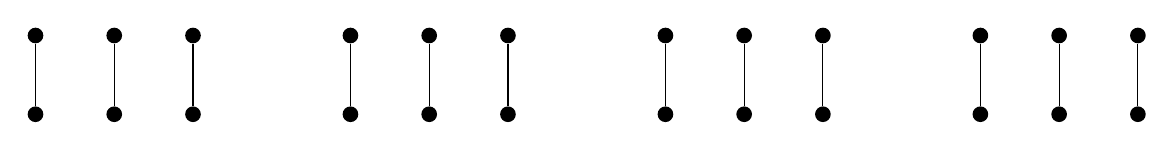
\begin{tikzpicture}
    \foreach\x in {0,1,2}{
        \node[fill, circle, inner sep=2pt] (a\x) at (\x,0) {};
        \node[fill, circle, inner sep=2pt] (b\x) at (\x,1) {};
        \draw (a\x) -- (b\x);
    }

    \foreach\x in {0,1,2}{
        \node[fill, circle, inner sep=2pt] (aa\x) at (\x+4,0) {};
        \node[fill, circle, inner sep=2pt] (bb\x) at (\x+4,1) {};
        \draw (aa\x) -- (bb\x);
    }

    \foreach\x in {0,1,2}{
        \node[fill, circle, inner sep=2pt] (aaa\x) at (\x+8,0) {};
        \node[fill, circle, inner sep=2pt] (bbb\x) at (\x+8,1) {};
        \draw (aaa\x) -- (bbb\x);
    }

    \foreach\x in {0,1,2}{
        \node[fill, circle, inner sep=2pt] (aaaa\x) at (\x+12,0) {};
        \node[fill, circle, inner sep=2pt] (bbbb\x) at (\x+12,1) {};
        \draw (aaaa\x) -- (bbbb\x);
    }


    \tube{a0}{1}
    \tube{a1}{1}
    \tube{a2}{1}
    
    \tube{bb0}{1}
    \tube{aa1}{1}
    \tube{aa2}{1}

    \tube{bbb0}{1}
    \tube{bbb1}{1}
    \tube{aaa2}{1}

    \tube{bbbb0}{1}
    \tube{bbbb1}{1}
    \tube{bbbb2}{1}

    \begin{scope}[xshift=.5cm, yshift=2cm]
        \cube
    \end{scope}
    \tube{000}{1}

    \begin{scope}[xshift=4.5cm, yshift=2cm]
        \cube
    \end{scope}
    \tube{100}{1}

    \begin{scope}[xshift=8.5cm, yshift=2cm]
        \cube
    \end{scope}
    \tube{110}{1}

    \begin{scope}[xshift=12.5cm, yshift=2cm]
        \cube
    \end{scope}
    \tube{111}{1}

    
\end{tikzpicture}
	\caption{The cube as a graph associahedron of disjoint edges. Adjacent tubings shown are related by flipping a tube and hence form an edge of the cube.}
	\label{fig:cube_graph_asso}
\end{figure}

\begin{figure}
	\centering
	% --- GLOBAL VARIABLES ---
\newcommand{\baseradius}{4}
\newcommand{\tubeborder}{.8}
% \tube{<comma separated list of coordinate/node names, e.g. A,B,C,A,D,E,C>}{<nesting depth>}
%
% Draws a tube (blue outline, white interior) of radius \baseradius + 2*(depth) pt
% around the closed polygonal path through the listed points, filling its interior
% (as the original version did via \filldraw ... -- cycle).
%
% Improvements over the original:
%  * The path is assembled *outside* the path parser (the original \ifnum inside
%    \filldraw silently lost the initial moveto, so nothing between the vertices
%    was ever drawn).
%  * All radii and line widths are measured in canvas pt while the coordinate
%    transformation is reset (\pgftransformreset). Node coordinates are stored
%    absolutely, so vertex disks stay perfect circles and their radius equals the
%    half-width of the stroked segments exactly. Hence the boundary is a single
%    C^1 curve (disks tangent to the straight strips), and this remains true when
%    the picture is scaled -- also separately in x and y. Only positions scale;
%    tube thickness and ring spacing stay constant, consistent across a document.
\newcommand{\tube}[2]{%
\begin{scope}[on background layer]
    \pgfmathsetmacro{\currentradius}{\baseradius + (#2 * 2)}%
    % assemble "(v1) -- (v2) -- ..." and count the vertices
    \gdef\tubepath{}\gdef\tubecount{0}%
    \foreach \v [count=\c] in {#1}{%
        \ifnum\c=1 \xdef\tubepath{(\v.center)}\else\xdef\tubepath{\tubepath -- (\v.center)}\fi
        \xdef\tubecount{\c}%
    }%
    \pgftransformreset % radii/line widths below are true canvas lengths
    \foreach \v in {#1}{\fill[Blue] (\v) circle (\currentradius pt);}%
    \ifnum\tubecount>1
        \filldraw[Blue, line width = 2*\currentradius pt, line join=round]
            \tubepath -- cycle;
    \fi
    \foreach \v in {#1}{\fill[white] (\v) circle (\currentradius pt - \tubeborder pt);}%
    \ifnum\tubecount>1
        \filldraw[white, line width = 2*\currentradius pt - 2*\tubeborder pt, line join=round]
            \tubepath -- cycle;
    \fi
\end{scope}
}
% a copy of the path P4 with vertices (#1-1)...(#1-4), centered at the current origin
\newcommand{\pathgraph}[1]{
    \foreach\x in {1,2,3,4}{
        \node[fill, circle, inner sep=1.5pt] (#1-\x) at ({(\x-2.5)*0.5},0) {};
    }
    \draw (#1-1) -- (#1-4);
}

\begin{tikzpicture}
    % invisible boxes at the vertices of the associahedron (used to clip the edges)
    \node[rectangle, minimum width=2.26cm, minimum height=0.88cm, inner sep=0pt] (box-1-12-123) at (-2.64,0.17) {};
    \node[rectangle, minimum width=2.26cm, minimum height=0.88cm, inner sep=0pt] (box-1-12-4) at (-0.83,-0.83) {};
    \node[rectangle, minimum width=2.26cm, minimum height=0.88cm, inner sep=0pt] (box-1-123-3) at (-1.50,1.50) {};
    \node[rectangle, minimum width=2.26cm, minimum height=0.88cm, inner sep=0pt] (box-1-3-34) at (-0.17,2.64) {};
    \node[rectangle, minimum width=2.26cm, minimum height=0.88cm, inner sep=0pt] (box-1-34-4) at (0.83,0.83) {};
    \node[rectangle, minimum width=2.26cm, minimum height=0.88cm, inner sep=0pt] (box-12-123-2) at (-2.34,-2.34) {};
    \node[rectangle, minimum width=2.26cm, minimum height=0.88cm, inner sep=0pt] (box-12-2-4) at (0.17,-2.64) {};
    \node[rectangle, minimum width=2.26cm, minimum height=0.88cm, inner sep=0pt] (box-123-2-23) at (-3.90,-3.90) {};
    \node[rectangle, minimum width=2.26cm, minimum height=0.88cm, inner sep=0pt] (box-123-23-3) at (-3.79,3.79) {};
    \node[rectangle, minimum width=2.26cm, minimum height=0.88cm, inner sep=0pt] (box-2-23-234) at (3.79,-3.79) {};
    \node[rectangle, minimum width=2.26cm, minimum height=0.88cm, inner sep=0pt] (box-2-234-4) at (1.50,-1.50) {};
    \node[rectangle, minimum width=2.26cm, minimum height=0.88cm, inner sep=0pt] (box-23-234-3) at (3.90,3.90) {};
    \node[rectangle, minimum width=2.26cm, minimum height=0.88cm, inner sep=0pt] (box-234-3-34) at (2.34,2.34) {};
    \node[rectangle, minimum width=2.26cm, minimum height=0.88cm, inner sep=0pt] (box-234-34-4) at (2.64,-0.17) {};
    % edges of the associahedron
    \draw (box-1-12-123) -- (box-1-12-4);
    \draw (box-1-12-123) -- (box-1-123-3);
    \draw (box-1-12-123) -- (box-12-123-2);
    \draw (box-1-12-4) -- (box-1-34-4);
    \draw (box-1-12-4) -- (box-12-2-4);
    \draw (box-1-123-3) -- (box-1-3-34);
    \draw (box-1-123-3) -- (box-123-23-3);
    \draw (box-1-3-34) -- (box-1-34-4);
    \draw (box-1-3-34) -- (box-234-3-34);
    \draw (box-1-34-4) -- (box-234-34-4);
    \draw (box-12-123-2) -- (box-12-2-4);
    \draw (box-12-123-2) -- (box-123-2-23);
    \draw (box-12-2-4) -- (box-2-234-4);
    \draw (box-123-2-23) -- (box-123-23-3);
    \draw (box-123-2-23) -- (box-2-23-234);
    \draw (box-123-23-3) -- (box-23-234-3);
    \draw (box-2-23-234) -- (box-2-234-4);
    \draw (box-2-23-234) -- (box-23-234-3);
    \draw (box-2-234-4) -- (box-234-34-4);
    \draw (box-23-234-3) -- (box-234-3-34);
    \draw (box-234-3-34) -- (box-234-34-4);
    % vertices of the associahedron = maximal tubings of the path
    \begin{scope}[shift={(-2.64,0.17)}]
        \pathgraph{1-12-123}
        \tube{1-12-123-1,1-12-123-3}{3}
        \tube{1-12-123-1,1-12-123-2}{2}
        \tube{1-12-123-1}{1}
    \end{scope}
    \begin{scope}[shift={(-0.83,-0.83)}]
        \pathgraph{1-12-4}
        \tube{1-12-4-1,1-12-4-2}{2}
        \tube{1-12-4-1}{1}
        \tube{1-12-4-4}{1}
    \end{scope}
    \begin{scope}[shift={(-1.50,1.50)}]
        \pathgraph{1-123-3}
        \tube{1-123-3-1,1-123-3-3}{2}
        \tube{1-123-3-1}{1}
        \tube{1-123-3-3}{1}
    \end{scope}
    \begin{scope}[shift={(-0.17,2.64)}]
        \pathgraph{1-3-34}
        \tube{1-3-34-3,1-3-34-4}{2}
        \tube{1-3-34-1}{1}
        \tube{1-3-34-3}{1}
    \end{scope}
    \begin{scope}[shift={(0.83,0.83)}]
        \pathgraph{1-34-4}
        \tube{1-34-4-3,1-34-4-4}{2}
        \tube{1-34-4-1}{1}
        \tube{1-34-4-4}{1}
    \end{scope}
    \begin{scope}[shift={(-2.34,-2.34)}]
        \pathgraph{12-123-2}
        \tube{12-123-2-1,12-123-2-3}{3}
        \tube{12-123-2-1,12-123-2-2}{2}
        \tube{12-123-2-2}{1}
    \end{scope}
    \begin{scope}[shift={(0.17,-2.64)}]
        \pathgraph{12-2-4}
        \tube{12-2-4-1,12-2-4-2}{2}
        \tube{12-2-4-2}{1}
        \tube{12-2-4-4}{1}
    \end{scope}
    \begin{scope}[shift={(-3.90,-3.90)}]
        \pathgraph{123-2-23}
        \tube{123-2-23-1,123-2-23-3}{3}
        \tube{123-2-23-2,123-2-23-3}{2}
        \tube{123-2-23-2}{1}
    \end{scope}
    \begin{scope}[shift={(-3.79,3.79)}]
        \pathgraph{123-23-3}
        \tube{123-23-3-1,123-23-3-3}{3}
        \tube{123-23-3-2,123-23-3-3}{2}
        \tube{123-23-3-3}{1}
    \end{scope}
    \begin{scope}[shift={(3.79,-3.79)}]
        \pathgraph{2-23-234}
        \tube{2-23-234-2,2-23-234-4}{3}
        \tube{2-23-234-2,2-23-234-3}{2}
        \tube{2-23-234-2}{1}
    \end{scope}
    \begin{scope}[shift={(1.50,-1.50)}]
        \pathgraph{2-234-4}
        \tube{2-234-4-2,2-234-4-4}{2}
        \tube{2-234-4-2}{1}
        \tube{2-234-4-4}{1}
    \end{scope}
    \begin{scope}[shift={(3.90,3.90)}]
        \pathgraph{23-234-3}
        \tube{23-234-3-2,23-234-3-4}{3}
        \tube{23-234-3-2,23-234-3-3}{2}
        \tube{23-234-3-3}{1}
    \end{scope}
    \begin{scope}[shift={(2.34,2.34)}]
        \pathgraph{234-3-34}
        \tube{234-3-34-2,234-3-34-4}{3}
        \tube{234-3-34-3,234-3-34-4}{2}
        \tube{234-3-34-3}{1}
    \end{scope}
    \begin{scope}[shift={(2.64,-0.17)}]
        \pathgraph{234-34-4}
        \tube{234-34-4-2,234-34-4-4}{3}
        \tube{234-34-4-3,234-34-4-4}{2}
        \tube{234-34-4-4}{1}
    \end{scope}
\end{tikzpicture}

	\caption{The classical associahedron as the graph associahedron of a path.}
	\label{fig:classical_asso_as_graph_asso}
\end{figure}

One of our main results concerns graph associahedra of trees. Here we give a brief introduction to the terminology of graph associahedra. See \cite{celebrating_associahedron} for a particularly well done introduction going into more detail.

Given a graph $G$, a \defn{tube} of $G$ is a subset $t\subset V(G)$ of the vertices of $G$ such that the induced subgraph $G[t]$ is connected and is not a connected component of $G$. Two tubes $t_1$ and $t_2$ with $t_1\ne t_2$ of $G$ are \defn{compatible}, if
\begin{itemize}
	\item $t_1\subset t_2$ or $t_2\subset t_1$. In this case we say that they are \defn{nested},
	\item or the induced subgraph $G[t_1\cup t_2]$ is not connected. Note that this implies $t_1\cap t_2=\emptyset$.
\end{itemize}
A \defn{tubing} of $G$ is a set of pairwise compatible tubes of $G$. A tubing is called \defn{nested}, if its tubes are pairwise nested. The \defn{graph associahedron} $\mathcal A(G)$ of $G$ is a polytope whose non-empty faces correspond to the tubings of $G$ with the reverse inclusion relation; adjoining the empty face gives its face lattice. I.e. the vertices of $\mathcal A(G)$ are the maximal tubings, edges correspond to tubings with one fewer tube than a maximal tubing, and facets correspond to tubings consisting of a single tube. It can be shown that for an $n$-vertex connected graph $G$, any maximal tubing consists of $n-1$ tubes. The maximal tubings of $G$ are in bijection to \defn{elimination trees} of $G$. An elimination tree of $G$ has any vertex $v$ of $G$ as a root. To this root we attach elimination trees of the connected components of $G\setminus\{v\}$. Given any maximal tubing of $G$, it can be shown that any tube in it can be replaced by a unique other tube to obtain another valid maximal tubing. This flip operation is another description of the edges of $\mathcal A(G)$ and it implies that graph associahedra are simple polytopes. In the language of elimination trees these flips correspond to tree rotations.

Many well known polytopes are special cases of graph associahedra. For example, when $G$ is a disjoint collection of $n$ edges, then any maximal tubing picks a singleton tube on each of these edges. This can be interpreted as a bit vector, saving the information about which vertex was picked on each edge. The corresponding polytope is then the $n$-dimensional cube, see \Cref{fig:cube_graph_asso}. When $G$ is the complete graph $K_n$, then any tubing of $G$ is nested. A maximal tubing of $K_n$ then consists of tubes $\{v_1\},\{v_1,v_2\},\ldots,\{v_1,v_2,\ldots,v_{n-1}\}$, which can be interpreted as the permutation $v_1,\ldots,v_n$ of the vertices. Hence, $\mathcal A(K_n)$ is the $(n-1)$-dimensional permutahedron. More generally, any nested and maximal tubing of a graph can be associated to a permutation of its vertices.

The classical associahedron is obtained by setting $G$ to be a path, see \Cref{fig:classical_asso_as_graph_asso}. A tubing of a path is easily identified as a valid bracketing, giving the bijection to Catalan objects. Setting $G$ to be a cycle gives the cyclohedron \cite{Cyclohedra, Cyclohedra_diameter} and setting $G$ to be a star gives the stellohedron \cite{stellohedron}, both of which are widely studied. Note that the classical associahedron and the stellohedron are obtained by setting $G$ to be a tree. A graph associahedron of a tree is called a \defn{tree associahedron}.

See also \cite{Graph_associahedra_diameter, Graph_associahedra_general, graph_properties_graph_associahedra, Graph_associahedra_realization, Elimination_trees} for further reading.

Let $T$ be a tree with root $r$. The facet-Hamiltonian path we will construct on $\mathcal A(T)$ will end in a maximal tubing called the \defn{bottom-up tubing}. It consists of the descendant sets of all vertices other than $r$, where a vertex belongs to its own descendant set. Equivalently, contract the edges incident to leaves other than the root, construct the bottom-up tubing of the contracted tree, and lift it back to $T$, adding the leaves as singleton tubes. We will show later that from the bottom-up tubing, we can flip greedily to any nested tubing coming from a DFS ordering.

\subsection{Rhombic Strips}

Given a graded poset $P$ with 0 and 1, a \defn{rhombic strip} of $P$ is a sub-drawing $R$ of a diagram of $P$ on the sphere with the following three properties:
\begin{itemize}
	\item $R$ is connected and spans all elements of $P$.
	\item $R$ is drawn crossing free, and the elements of $P$ of a common rank are drawn on a common circle of latitude. The 0 and 1 of $P$ are placed at the south- and north pole, respectively.
	\item All faces of $R$ have degree 4 (are rhombi), except possibly one designated \defn{outer face}, which is bounded by two maximal chains connecting 0 and 1.
\end{itemize}

The two chains bounding the outer face are called the \defn{left and right boundaries of $R$}. They may share vertices and edges. A rhombic strip is \defn{cyclic} if it does not have an outer face.

A rhombic strip is called \defn{Hamiltonian} if it contains a Hamilton path (cycle) which visits the elements of $P$ of any given rank $k$ in the order they appear on their circle of latitude. For a cyclic rhombic strip we require a Hamilton cycle, for a non-cyclic rhombic strip we require a Hamilton path.

A \defn{rhombus} is a face of $R$ that is bounded by four elements of $P$, two of which have rank $k$, one has rank $k+1$ and the remaining one has rank $k-1$. The \defn{rank of that rhombus} is $k$.

We call a path or cycle $\gamma\subset S^2$ on the 2-sphere \defn{$c$-monotone} if every open great half circle connecting the north and south poles intersects $\gamma$ at most once. Equivalently, the longitude projection is injective on $\gamma$ with the poles removed.
\begin{observation}
	A Hamiltonian rhombic strip can be drawn such that its Hamilton path or cycle is $c$-monotone, by changing the position of the vertices on their circles of latitude, but not their order.
\end{observation}

\section{Related work}\label{sec:related}

\begin{figure}
	\centering
	
\thispagestyle{empty}

\begin{tikzpicture}[scale = 0.5, every node/.style={font=\scriptsize}]

\coordinate (empty) at (6,-2);

\coordinate (1) at (2,0);
\coordinate (2) at (4,0);
\coordinate (3) at (6,0);
\coordinate (4) at (10,0);

\coordinate (12) at (2,2);
\coordinate (23) at (4,2);
\coordinate (13) at (6,2);
\coordinate (34) at (8,2);
\coordinate (24) at (10,2);
\coordinate (14) at (12,2);

\coordinate (123) at (4,4);
\coordinate (134) at (8,4);
\coordinate (234) at (10,4);
\coordinate (124) at (12,4);

\coordinate (1234) at (8,6);

\fill[Green] (empty) -- (1) -- (12) -- (2);
\fill[Orange] (2) -- (12) -- (123) -- (23);
\fill[Blue] (empty) -- (2) -- (23) -- (3);
\fill[Vermilion] (3) -- (23) -- (123) -- (13);
\fill[Purple] (13) -- (123) -- (1234) -- (134);

\foreach \a/\b in {empty/1,empty/2,empty/3,empty/4,1/12,2/12,2/23,3/23,3/13,3/34,4/34,4/24,4/14,12/123,23/123,13/123,13/134,34/134,34/234,24/234,24/124,14/124,1234/123,1234/124,1234/134,1234/234}
{  \draw (\a) -- (\b);  }

\foreach\n in {1,2,3,4,12,13,14,23,24,34,123,124,134,234,1234}
{ \node[draw, fill = white] at (\n) {$\n$}; }
\node[draw, fill = white] at (empty) {$\emptyset$};

\end{tikzpicture}
	\caption{A rhombic strip of $\mathcal B_4$ with some colorfully marked rhombi. The maximal chains represent permutations, and a flip across a rhombus represents an adjacent transposition. The left boundary represents 1234. Flipping across the green rhombus, we obtain 2134. Then, flipping orange, blue, red and finally purple, we obtain 2314, 3214, 3124 and finally 3142. This rhombic strip represents a facet-Hamiltonian path of the 3 dimensional permutahedron. The facet-Hamiltonian path is depicted in \Cref{fig:perm as truncation}.}
	\label{fig:rhombic to fh example}
\end{figure}

\paragraph{Facet-Hamiltonicity}
Rhombic strips were originally introduced by \textcite{facethamiltonicity} as an encoding of \defn{facet-Hamiltonian} paths and cycles. A facet-Hamiltonian path (or cycle) on a polytope $\mathcal P$ is a path (or cycle) $C$ on $\mathcal P$ such that the intersection $C\cap f$ is non-empty and connected for all facets $f$ of $\mathcal P$. They are optimal watchman routes for the facets of a polytope when restricting the watchman to its skeleton \cite{watchmanChin, watchmanLines, watchmanSimple, watchmanApproximation}. Furthermore, they are versions of non-revisiting cycles and hence connected to the Hirsch conjecture, see \cite{non-revisiting1, non-revisiting2, non-revisiting3, non-revisiting4, non-revisiting5}.

As an example, consider the \defn{permutahedron}. It can be defined to be the convex hull of the set of permutations of $[n]$ viewed as integer vectors. For example, the 2-dimensional permutahedron would be the convex hull of
\[
	(1,2,3),(1,3,2),(3,1,2),(3,2,1),(2,3,1),(2,1,3).
\]
Here, we do not care about the specific realization of the polytope, but only about its face lattice. The faces of the permutahedron consist of ordered set partitions of $[n]$. A partition into $k$ sets has dimension $n-k$. For example, the partitions into $n$ subsets consist of singleton sets, like $\{1\},\{3\},\{4\},\{2\}$. These are the vertices of the permutahedron and they correspond to permutations. Edges contain exactly one set of two elements in their associated partition. For example, the edge $\{1\},\{3,4\},\{2\}$ connects the vertices $\{1\},\{3\},\{4\},\{2\}$ and $\{1\},\{4\},\{3\},\{2\}$. Hence, edges correspond to adjacent transpositions. The facets consist of a partition into two sets. Ignoring the second set, they correspond to the non-empty and proper subsets of $[n]$. See also \Cref{fig:perm as truncation}. In the preliminaries we claimed that the permutahedron is the graph associahedron of a complete graph. Indeed, when labeling the vertices of $K_n$ by $1,\ldots,n$, a tube is any subset of $[n]$ and because all tubings are nested, they are ordered partitions of $[n]$.

The permutahedron is a very well studied polytope \cite{Permutahedra_associahedra_beyond, Permutahedron_and_gen_associahedron}. A facet-Hamiltonian cycle on the permutahedron is a cyclic listing of permutations such that adjacent permutations differ in adjacent transpositions and the set of permutations sharing a fixed subset as a prefix form a connected arc along the listing. The facet-Hamiltonian cycles of the permutahedron correspond to rhombic strips of $\mathcal B_n$, because the maximal chains of $\mathcal B_n$ correspond to permutations. Flipping such a chain across a rhombus of a rhombic strip corresponds to an adjacent transposition. See \Cref{fig:rhombic to fh example} for a visualization or \cite{facethamiltonicity} for more details.

\paragraph{Omnitruncation and Graph Associahedra}
The correspondence between facet-Hamiltonian paths and cycles and rhombic strips extends to more posets. Given some polytope $P$, we define its \defn{omnitruncation} $\tr(P)$ to be the polytope obtained by truncating all non-empty proper faces of $P$. It has the flags of $P$ as vertices and the non-empty proper faces of $P$ as facets. It is well known that the omnitruncation of the simplex is the permutahedron. And since the face lattice of the simplex is $\mathcal B_n$, this construction generalizes the considerations of the previous paragraph. We obtain
\begin{lemma}[\cite{facethamiltonicity}]
	Let $P$ be any polytope. The facet-Hamiltonian paths (cycles) of $\tr(P)$ correspond to (cyclic) rhombic strips of the face lattice of $P$.
\end{lemma}

\begin{figure}
	\centering
	\begin{subfigure}[b]{0.49\textwidth}
		\centering
		

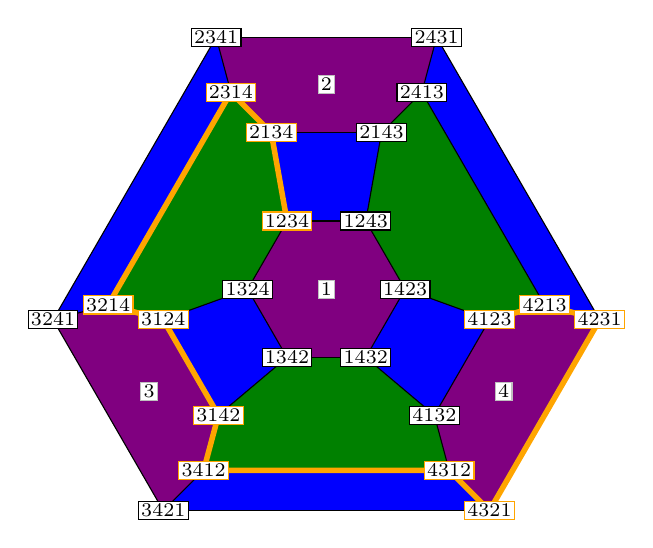
\begin{tikzpicture}[scale=2, every node/.style={font=\scriptsize, inner sep=1pt}]
        
\coordinate (1) at (0,0);
\coordinate (2) at (90:1.6);
\coordinate (3) at (210:1.6);
\coordinate (4) at (-30:1.6);

\coordinate (1a) at (0,0);
\coordinate (2a) at (90:1.3);
\coordinate (3a) at (210:1.3);
\coordinate (4a) at (-30:1.3);
        
\def\r{0.5}
\coordinate (1234) at (120:\r);
\coordinate (1324) at (180:\r);
\coordinate (1342) at (240:\r);
\coordinate (1432) at (300:\r);
\coordinate (1423) at (0:\r);
\coordinate (1243) at (60:\r);
\def\r{0.7}
\coordinate (2134) at ($(2)+(-90-30:\r)$);
\coordinate (2314) at ($(2)+(-90-60:\r)$);
\coordinate (2341) at ($(2)+(-90-90:\r)$);
\coordinate (2431) at ($(2)+(-90+90:\r)$);
\coordinate (2143) at ($(2)+(-90+30:\r)$);
\coordinate (2413) at ($(2)+(-90+60:\r)$);

\coordinate (3124) at ($(3)+(30+30:\r)$);
\coordinate (3214) at ($(3)+(30+60:\r)$);
\coordinate (3241) at ($(3)+(30+90:\r)$);
\coordinate (3421) at ($(3)+(30-90:\r)$);
\coordinate (3142) at ($(3)+(30-30:\r)$);
\coordinate (3412) at ($(3)+(30-60:\r)$);

\coordinate (4123) at ($(4)+(150-30:\r)$);
\coordinate (4213) at ($(4)+(150-60:\r)$);
\coordinate (4231) at ($(4)+(150-90:\r)$);
\coordinate (4321) at ($(4)+(150+90:\r)$);
\coordinate (4132) at ($(4)+(150+30:\r)$);
\coordinate (4312) at ($(4)+(150+60:\r)$);

% vertices 
\foreach\a/\b/\c/\d in {1/2/3/4, 2/1/3/4, 3/1/2/4, 4/1/2/3}
{
    \fill[Purple] (\a\b\c\d) -- (\a\b\d\c) -- (\a\d\b\c) -- (\a\d\c\b) -- (\a\c\d\b) -- (\a\c\b\d);
}

% edges
\foreach\a/\b/\c/\d in {1/2/3/4, 1/3/2/4, 1/4/2/3, 2/3/1/4, 2/4/1/3, 3/4/1/2}
{
    \fill[Blue] (\a\b\c\d) -- (\b\a\c\d) -- (\b\a\d\c) -- (\a\b\d\c);
}

% faces
\foreach\a/\b/\c/\d in {2/1/3/4, 3/1/2/4, 4/1/2/3}
{
    \fill[Green] (\b\c\d\a) -- (\b\d\c\a) -- (\d\b\c\a) -- (\d\c\b\a) -- (\c\d\b\a) -- (\c\b\d\a);
}

\foreach\x in {1,2,3,4} {
    \node at (\x a) [draw=gray!50!white, rectangle, fill=white] {$\x$};
}

\foreach\a/\b in {
1234/1243,
1234/1324,
1234/2134,
1243/1423,
1243/2143,
1423/4123,
1423/1432,
4123/4132,
4123/4213,
4132/1432,
4132/4312,
1432/1342,
1342/1324,
1342/3142,
1324/3124,
3124/3142,
3124/3214,
3142/3412,
3412/4312,
3412/3421,
4312/4321,
4321/3421,
4321/4231,
3421/3241,
3241/3214,
3241/2341,
3214/2314,
2314/2341,
2314/2134,
2341/2431,
2431/4231,
2431/2413,
4231/4213,
4213/2413,
2413/2143,
2143/2134}{
    \draw (\a) -- (\b);
}

\draw[line width=2pt, Orange] (1234) -- (2134) -- (2314) -- (3214)-- (3124) -- (3142) -- (3412) -- (4312) -- (4321) -- (4231) -- (4213) -- (4123);

\foreach\x in {1234,1324,1342,1432,1423,1243,2134,2143,2413,2431,2341,2314,3124,3214,3241,3421,3412,3142,4123,4213,4231,4321,4312,4132}
{
    \node at (\x) [draw, rectangle, fill=white] {$\x$};
}
\foreach\x in {1234,2134, 2314, 3214, 3124, 3142, 3412, 4312, 4321, 4231, 4213, 4123}
{
    \node at (\x) [draw=Orange, rectangle, fill=white] {$\x$};
}
\end{tikzpicture}
		\caption{The vertices of the simplex are labeled $1,2,3,4$. Faces of the permutahedron. The facet-Hamiltonian path induced by the rhombic strip in \Cref{fig:rhombic to fh example} is drawn in orange. Note that it can be closed to a facet-Hamiltonian cycle.}
		\label{fig:perm as truncation}
	\end{subfigure}
	\hfill
	\begin{subfigure}[b]{0.49\textwidth}
		\centering
		% Plane graph of the omnitruncated 3-cube (truncated cuboctahedron).
% Each vertex is labeled by its own coordinate vector x = x1 x2 x3,
% a signed permutation of 123 (a bar over position i means x_i < 0).
%   Purple hexagons  <-> vertices of the cube:  fixed sign vector (bar pattern by POSITION)
%   Blue   squares   <-> edges of the cube:     the two entries of magnitude 2,3 sit in
%                                               two fixed positions with fixed signs
%   Green  octagons  <-> facets of the cube:    the entry +-3 sits in a fixed position
%                                               with fixed sign; x3 = -3 is the outer face.
% Two vertices are adjacent iff they differ by swapping the magnitudes k,k+1 in place
% (signs stay with the positions) or by flipping the sign of the entry +-1.
% Requires: \usepackage[dvipsnames]{xcolor}, \usepackage{tikz}
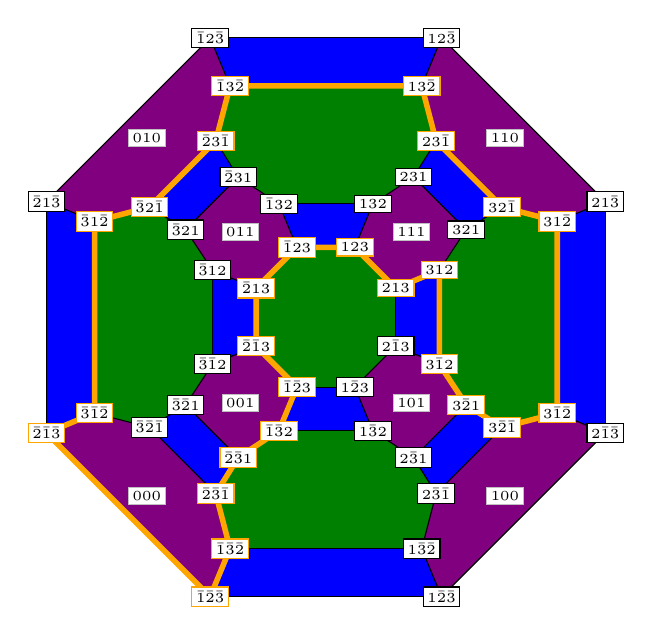
\begin{tikzpicture}[scale=1.2, every node/.style={font=\tiny, inner sep=1.5pt}]

% radii of the six concentric rings (= levels x3 = 3,2,1,-1,-2,-3)
\def\rA{0.80}\def\rB{1.30}\def\rC{1.75}\def\rD{2.20}\def\rE{2.65}\def\rF{3.20}

% ring 1: octagon of the facet x3 = +1  (vertices with x3 = 3)
\foreach \n/\a in {213/22.5, 123/67.5, n123/112.5, n213/157.5,
                   n2n13/202.5, n1n23/247.5, 1n23/292.5, 2n13/337.5}
  \coordinate (\n) at (\a:\rA);
% ring 2: vertices with x3 = 2
\foreach \n/\a in {312/22.5, 132/67.5, n132/112.5, n312/157.5,
                   n3n12/202.5, n1n32/247.5, 1n32/292.5, 3n12/337.5}
  \coordinate (\n) at (\a:\rB);
% ring 3: vertices with x3 = 1
\foreach \n/\a in {321/32, 231/58, n231/122, n321/148,
                   n3n21/212, n2n31/238, 2n31/302, 3n21/328}
  \coordinate (\n) at (\a:\rC);
% ring 4: vertices with x3 = -1
\foreach \n/\a in {32n1/32, 23n1/58, n23n1/122, n32n1/148,
                   n3n2n1/212, n2n3n1/238, 2n3n1/302, 3n2n1/328}
  \coordinate (\n) at (\a:\rD);
% ring 5: vertices with x3 = -2
\foreach \n/\a in {31n2/22.5, 13n2/67.5, n13n2/112.5, n31n2/157.5,
                   n3n1n2/202.5, n1n3n2/247.5, 1n3n2/292.5, 3n1n2/337.5}
  \coordinate (\n) at (\a:\rE);
% ring 6: octagon of the facet x3 = -1 (vertices with x3 = -3), the outer face
\foreach \n/\a in {21n3/22.5, 12n3/67.5, n12n3/112.5, n21n3/157.5,
                   n2n1n3/202.5, n1n2n3/247.5, 1n2n3/292.5, 2n1n3/337.5}
  \coordinate (\n) at (\a:\rF);

% vertices of the cube: hexagons (fixed bar pattern)
\foreach \pa/\pb/\pc/\pd/\pe/\pf in {
  213/123/132/231/321/312,
  n123/n213/n312/n321/n231/n132,
  n2n13/n1n23/n1n32/n2n31/n3n21/n3n12,
  1n23/1n32/2n31/3n21/3n12/2n13,
  21n3/12n3/13n2/23n1/32n1/31n2,
  n12n3/n21n3/n31n2/n32n1/n23n1/n13n2,
  n2n1n3/n1n2n3/n1n3n2/n2n3n1/n3n2n1/n3n1n2,
  1n2n3/2n1n3/3n1n2/3n2n1/2n3n1/1n3n2}
{
  \fill[Purple] (\pa) -- (\pb) -- (\pc) -- (\pd) -- (\pe) -- (\pf) -- cycle;
}
% edges of the cube: squares
\foreach \pa/\pb/\pc/\pd in {
  213/312/3n12/2n13,
  123/132/n132/n123,
  n213/n312/n3n12/n2n13,
  1n23/1n32/n1n32/n1n23,
  321/231/23n1/32n1,
  n231/n321/n32n1/n23n1,
  n3n21/n2n31/n2n3n1/n3n2n1,
  2n31/3n21/3n2n1/2n3n1,
  21n3/31n2/3n1n2/2n1n3,
  12n3/13n2/n13n2/n12n3,
  n21n3/n31n2/n3n1n2/n2n1n3,
  1n2n3/1n3n2/n1n3n2/n1n2n3}
{
  \fill[Blue] (\pa) -- (\pb) -- (\pc) -- (\pd) -- cycle;
}
% facets of the cube: octagons (the sixth one, x3 = -1, is the outer face)
\foreach \pa/\pb/\pc/\pd/\pe/\pf/\pg/\ph in {
  213/123/n123/n213/n2n13/n1n23/1n23/2n13,
  312/321/32n1/31n2/3n1n2/3n2n1/3n21/3n12,
  132/231/23n1/13n2/n13n2/n23n1/n231/n132,
  n312/n321/n32n1/n31n2/n3n1n2/n3n2n1/n3n21/n3n12,
  1n32/2n31/2n3n1/1n3n2/n1n3n2/n2n3n1/n2n31/n1n32}
{
  \fill[Green] (\pa) -- (\pb) -- (\pc) -- (\pd) -- (\pe) -- (\pf) -- (\pg) -- (\ph) -- cycle;
}

% cube-vertex labels (analogue of the gray 1,2,3,4 boxes)
\foreach \a/\l in {45/{111}, 135/{011}, 225/{001}, 315/{101}}
  \node at (\a:1.28) [draw=gray!50!white, rectangle, fill=white] {$\l$};
\foreach \a/\l in {45/{110}, 135/{010}, 225/{000}, 315/{100}}
  \node at (\a:2.68) [draw=gray!50!white, rectangle, fill=white] {$\l$};

% the 72 edges
\foreach \a/\b in {
% swaps of the magnitudes 2 <-> 3 (between a square and a hexagon)
213/312, 123/132, n123/n132, n213/n312, n2n13/n3n12, n1n23/n1n32, 1n23/1n32, 2n13/3n12,
321/231, n231/n321, n3n21/n2n31, 2n31/3n21,
32n1/23n1, n23n1/n32n1, n3n2n1/n2n3n1, 2n3n1/3n2n1,
31n2/21n3, 13n2/12n3, n13n2/n12n3, n31n2/n21n3, n3n1n2/n2n1n3, n1n3n2/n1n2n3, 1n3n2/1n2n3, 3n1n2/2n1n3,
% swaps of the magnitudes 1 <-> 2 (between an octagon and a hexagon)
213/123, n123/n213, n2n13/n1n23, 1n23/2n13,
312/321, 132/231, n132/n231, n312/n321, n3n12/n3n21, n1n32/n2n31, 1n32/2n31, 3n12/3n21,
32n1/31n2, 23n1/13n2, n23n1/n13n2, n32n1/n31n2, n3n2n1/n3n1n2, n2n3n1/n1n3n2, 2n3n1/1n3n2, 3n2n1/3n1n2,
21n3/12n3, n12n3/n21n3, n2n1n3/n1n2n3, 1n2n3/2n1n3,
% sign flips of the entry +-1 (between an octagon and a square)
123/n123, n213/n2n13, n1n23/1n23, 2n13/213,
312/3n12, 132/n132, n312/n3n12, 1n32/n1n32,
321/32n1, 231/23n1, n231/n23n1, n321/n32n1, n3n21/n3n2n1, n2n31/n2n3n1, 2n31/2n3n1, 3n21/3n2n1,
31n2/3n1n2, 13n2/n13n2, n31n2/n3n1n2, 1n3n2/n1n3n2,
21n3/2n1n3, 12n3/n12n3, n21n3/n2n1n3, n1n2n3/1n2n3}
{
  \draw (\a) -- (\b);
}

% fh cycle
\draw[line width=2pt, Orange];

% vertex labels (coordinate vectors)
\foreach \n/\l in {
213/213, 123/123, n123/\bar123, n213/\bar213, n2n13/\bar2\bar13, n1n23/\bar1\bar23, 1n23/1\bar23, 2n13/2\bar13,
312/312, 132/132, n132/\bar132, n312/\bar312, n3n12/\bar3\bar12, n1n32/\bar1\bar32, 1n32/1\bar32, 3n12/3\bar12,
321/321, 231/231, n231/\bar231, n321/\bar321, n3n21/\bar3\bar21, n2n31/\bar2\bar31, 2n31/2\bar31, 3n21/3\bar21,
32n1/32\bar1, 23n1/23\bar1, n23n1/\bar23\bar1, n32n1/\bar32\bar1, n3n2n1/\bar3\bar2\bar1, n2n3n1/\bar2\bar3\bar1, 2n3n1/2\bar3\bar1, 3n2n1/3\bar2\bar1,
31n2/31\bar2, 13n2/13\bar2, n13n2/\bar13\bar2, n31n2/\bar31\bar2, n3n1n2/\bar3\bar1\bar2, n1n3n2/\bar1\bar3\bar2, 1n3n2/1\bar3\bar2, 3n1n2/3\bar1\bar2,
21n3/21\bar3, 12n3/12\bar3, n12n3/\bar12\bar3, n21n3/\bar21\bar3, n2n1n3/\bar2\bar1\bar3, n1n2n3/\bar1\bar2\bar3, 1n2n3/1\bar2\bar3, 2n1n3/2\bar1\bar3}
{
  \node at (\n) [draw, rectangle, fill=white] {$\l$};
}

\draw[line width=2pt, Orange] (213) -- (123) -- (n123) -- (n213) -- (n2n13)
  -- (n1n23) -- (n1n32) -- (n2n31) -- (n2n3n1) -- (n1n3n2) -- (n1n2n3)
  -- (n2n1n3) -- (n3n1n2) -- (n31n2) -- (n32n1) -- (n23n1) -- (n13n2)
  -- (13n2) -- (23n1) -- (32n1) -- (31n2) -- (3n1n2) -- (3n2n1)
  -- (3n21) -- (3n12) -- (312) -- cycle;

\foreach \n/\l in {
213/213, 123/123, n123/\bar123, n213/\bar213, n2n13/\bar2\bar13, n1n23/\bar1\bar23, n1n32/\bar1\bar32,
n2n31/\bar2\bar31, n2n3n1/\bar2\bar3\bar1, n1n3n2/\bar1\bar3\bar2, n1n2n3/\bar1\bar2\bar3, n2n1n3/\bar2\bar1\bar3, n3n1n2/\bar3\bar1\bar2, n31n2/\bar31\bar2,
n32n1/\bar32\bar1, n23n1/\bar23\bar1, n13n2/\bar13\bar2, 13n2/13\bar2, 23n1/23\bar1, 32n1/32\bar1, 31n2/31\bar2,
3n1n2/3\bar1\bar2, 3n2n1/3\bar2\bar1, 3n21/3\bar21, 3n12/3\bar12, 312/312}
{
    \node at (\n) [draw=Orange, rectangle, fill=white] {$\l$};
}
\end{tikzpicture}

		\caption{The 3 dimensional $B$-permutahedron as the omnitruncation of the 3 dimensional cube. A facet-Hamiltonian cycle is highlighted in orange.}
		\label{fig:Bperm}
	\end{subfigure}
	\caption{The 3 dimensional permutahedron (\textsc{a}) and $B$-permutahedron (\textsc{b}) as omnitruncations of the 3 dimensional simplex and cube, respectively. Faces of the omnitruncation resulting from vertices, edges and faces of the truncated polytope are purple, blue and green, respectively.}
	\label{fig:omnitruncation}
\end{figure}
For a connected graph $G$, we consider the poset of its tubes under inclusion, with $\emptyset$ and $V(G)$ adjoined as 0 and 1. Its maximal chains, after omitting these two extremes, correspond to maximal nested tubings of $G$. A (cyclic) rhombic strip of this poset hence corresponds to a facet-Hamiltonian path (cycle) of $\mathcal A(G)$.

\paragraph{The $B$-Permutahedron}
Recently, \textcite{Listing_faces} have conjectured that the face lattice of any polytope has a Hamilton cycle. They give evidence for their conjecture by confirming it for a number of well known polytopes. To obtain a Hamilton cycle in the face lattice of an $n$-dimensional cube, they put in some extra work and actually construct a Hamiltonian rhombic strip of this face lattice. Their construction is very similar to a combination of unfolding and zigzagging as we define them here, and it directly inspired this work. The omnitruncation of the cube is known as the $B$-permutahedron, see \Cref{fig:Bperm}. Its vertices can be associated to signed permutations and its facets to faces of the cube. The construction of a rhombic strip for the face lattice of the cube hence resolved the conjecture by \textcite{facethamiltonicity} that states that the $B$-permutahedron should admit a facet-Hamiltonian cycle.

\begin{figure}
	\centering
	
% Custom tube command
\newcommand{\tube}[1]{%
\begin{tikzpicture}[scale = 0.15]
    \IfSubStr{#1}{a}{ \fill[Blue, draw] (0,4.5) circle (8pt); }{ \draw (0,4.5) circle (8pt); }
    \IfSubStr{#1}{b}{ \fill[Blue, draw] (0,3) circle (8pt); }{ \draw (0,3) circle (8pt); }
    \IfSubStr{#1}{c}{ \fill[Blue, draw] (0,1.5) circle (8pt); }{ \draw (0,1.5) circle (8pt); }
    \IfSubStr{#1}{x}{ \fill[Blue, draw] (1,4.5) circle (8pt); }{ \draw (1,4.5) circle (8pt); }
    \IfSubStr{#1}{y}{ \fill[Blue, draw] (1,3) circle (8pt); }{ \draw (1,3) circle (8pt); }
    \IfSubStr{#1}{z}{ \fill[Blue, draw] (1,1.5) circle (8pt); }{ \draw (1,1.5) circle (8pt); }
\end{tikzpicture}%
}

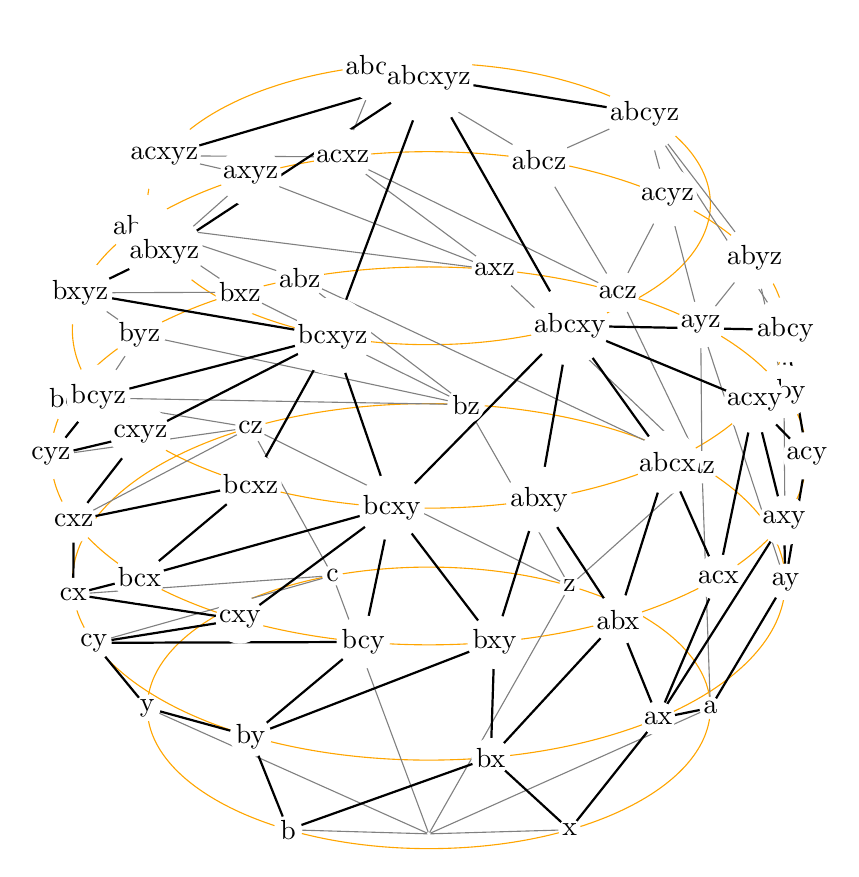
\begin{tikzpicture}[
    x={(1cm, 0cm)},
    y={(0cm, 0.5cm)},
    z={(0cm, 1cm)},
    scale=.8
]

\def\anglestep{20} % 18 steps * 20 degrees = 360 degree wrap-around

% 1. DRAW BACKGROUND SPHERICAL REFERENCE CIRCLES
\foreach \z/\r in {0/4.47, 2/5.66, 4/6, 6/5.66, 8/4.47}{
    \begin{scope}[canvas is xy plane at z=\z]
        \draw[Orange, thin] (0,0) circle[radius=\r];
    \end{scope}
}

% 2. DEFINE POLES
\coordinate (empty) at (0,0,-2);
\coordinate (abcxyz) at (0,0,10);

% 3. DEFINE EVENLY SPACED COORDINATES 
\begin{scope}[canvas is xy plane at z=0]
    % 6 nodes (spaced by 3)
    \foreach \name/\ax in {a/0, z/3, c/5.5, y/9, b/12, x/15} 
        \coordinate (\name) at (\ax*\anglestep:4.47);
\end{scope}

\begin{scope}[canvas is xy plane at z=2]
    % 9 nodes (spaced by 2)
    \foreach \name/\ax in {ay/0, az/2, bz/4.2, cz/6, cx/9.2, cy/10, by/12, bx/14, ax/15.5} 
        \coordinate (\name) at (\ax*\anglestep:5.66);
\end{scope}

\begin{scope}[canvas is xy plane at z=4]
    % 18 nodes (spaced by 1)
    \foreach \name/\ax in {acy/0, aby/1, ayz/2.2, acz/3, axz/4, abz/5.5, bxz/6, byz/7, bcz/8.1, cyz/9, cxz/10, bcx/11, cxy/12, bcy/13, bxy/14, abx/15, acx/16, axy/17} 
        \coordinate (\name) at (\ax*\anglestep:6);
\end{scope}

\begin{scope}[canvas is xy plane at z=6]
    % 15 nodes (spaced by 1.2)
    \foreach \name/\ax in {abcy/0, abyz/1.2, acyz/2.4, abcz/3.6, acxz/5.2, axyz/6.0, abxz/7.2, bxyz/8.4, bcyz/10.1, cxyz/10.8, bcxz/12.0, bcxy/13.2, abxy/14.4, abcx/15.6, acxy/16.8} 
        \coordinate (\name) at (\ax*\anglestep:5.66);
\end{scope}

\begin{scope}[canvas is xy plane at z=8]
    % 6 nodes (spaced by 3)
    \foreach \name/\ax in {abcyz/2, abcxz/5, acxyz/8, abxyz/10, bcxyz/12.5, abcxy/15} 
        \coordinate (\name) at (\ax*\anglestep:4.47);
\end{scope}


% 4. PRECOMPUTED EDGE LISTS 
\def\backedges{%
    empty/a, empty/c, empty/z,
    z/az, z/bz, z/cz, a/az, c/cz,
    az/ayz, az/acz, az/axz, az/abz,
    bz/abz, bz/bxz, bz/byz, bz/bcz,
    cz/bcz, cz/cyz,
    ay/aby, ay/ayz,
    ayz/abyz, ayz/acyz,
    acz/acyz, acz/abcz, acz/acxz,
    axz/acxz, axz/axyz, axz/abxz,
    abz/abxz, bxz/abxz, bxz/bxyz,
    byz/bxyz, 
    aby/abyz, abyz/abcyz,
    acyz/abcyz, abcz/abcyz, abcz/abcxz,
    axyz/abxyz,byz/bcyz,
    empty/b, empty/x, empty/y,
    acxz/abcxz, acxz/acxyz, axyz/acxyz,c/cx, c/cy,cz/cxz,
    abcy/abcyz%
}

\def\frontedges{%
    abcxyz/acxyz, abcxyz/abxyz, abcxyz/bcxyz, abcxyz/abcxy,abcxyz/abcyz, abcxyz/abcxz,
    a/ax, a/ay, bcz/bcyz,
    y/cy, y/by, b/by, b/bx, x/bx, x/ax,
      aby/abcy,
    ax/abx, ax/acx, ax/axy,
    ay/axy, ay/acy,
    cy/cxy, cy/bcy,
    by/bcy, by/bxy,
    bx/bxy, bx/abx,
    cyz/bcyz, cyz/cxyz,
    cxz/cxyz, cxz/bcxz,
    bcx/bcxz, bcx/bcxy,
    cxy/bcxy, bcy/bcxy, bxy/bcxy, bxy/abxy,
    abx/abxy, abx/abcx,
    acx/abcx, acx/acxy,
    axy/acxy, acy/acxy, acy/abcy,
    abxz/abxyz, bxyz/abxyz, bxyz/bcxyz,
    bcyz/bcxyz, cxyz/bcxyz, bcxz/bcxyz,
    bcxy/bcxyz, bcxy/abcxy,cx/cxz, cx/bcx, cx/cxy,
    abxy/abcxy, abcx/abcxy, acxy/abcxy, abcy/abcxy%
}

% Draw Back Edges (Thin, Gray)
\foreach \u/\v in \backedges {
    \draw[thin, gray] (\u) -- (\v);
}

% Draw Front Edges (Thick, Black)
\foreach \u/\v in \frontedges {
    \draw[thick, black] (\u) -- (\v);
}

% 5. PLACE ALL NODES ON TOP (Removes need for manual redraws later)
\foreach \n in {a,b,c,x,y,z,ax,ay,az,bx,by,bz,cx,cy,cz,abx,aby,abz,acx,acy,acz,bcx,bcy,bcz,axy,bxy,cxy,axz,bxz,cxz,ayz,byz,cyz,abcx,abcy,abcz,abxy,abxz,abyz,acxy,acxz,acyz,bcxy,bcxz,bcyz,axyz,bxyz,cxyz,abcxy,abcxz,abcyz,abxyz,acxyz,bcxyz} {
    \node[fill=white, circle, inner sep=0.5pt] at (\n) {\tube{\n}};
}

% Place Poles
\node[fill=white, circle, inner sep=0.5pt] at (empty) {\tube{}};
\node[fill=white, circle, inner sep=0.5pt] at (abcxyz) {\tube{abcxyz}};

\end{tikzpicture}
	\caption{The poset of connected induced subgraphs of $K_{3,3}$. Edges of $K_{3,3}$ are omitted for visibility. Circles of latitude are drawn in orange, indicating the ranks.}
	\label{fig:K33 on sphere}
\end{figure}

\begin{figure}
	\centering
	\makebox[\textwidth][c]{
\newcommand{\tube}[1]{
\begin{tikzpicture}[scale = 0.22]
    \IfSubStr{#1}{a}{ \fill[Blue, draw] (0,3) circle (8pt); }{ \draw (0,3) circle (8pt); }
    \IfSubStr{#1}{b}{ \fill[Blue, draw] (0,2) circle (8pt); }{ \draw (0,2) circle (8pt); }
    \IfSubStr{#1}{c}{ \fill[Blue, draw] (0,1) circle (8pt); }{ \draw (0,1) circle (8pt); }
    \IfSubStr{#1}{x}{ \fill[Blue, draw] (1,3) circle (8pt); }{ \draw (1,3) circle (8pt); }
    \IfSubStr{#1}{y}{ \fill[Blue, draw] (1,2) circle (8pt); }{ \draw (1,2) circle (8pt); }
    \IfSubStr{#1}{z}{ \fill[Blue, draw] (1,1) circle (8pt); }{ \draw (1,1) circle (8pt); }
\end{tikzpicture}
}
\newcommand{\bound}{
\begin{tikzpicture}[scale = 0.29, xscale = 1.3]
    \fill[white] (0,1) -- (1,1) -- (1,3) -- (0,3) -- cycle;
\end{tikzpicture}
}
\newcommand{\clrone}{Blue}
\newcommand{\clrtwo}{red}



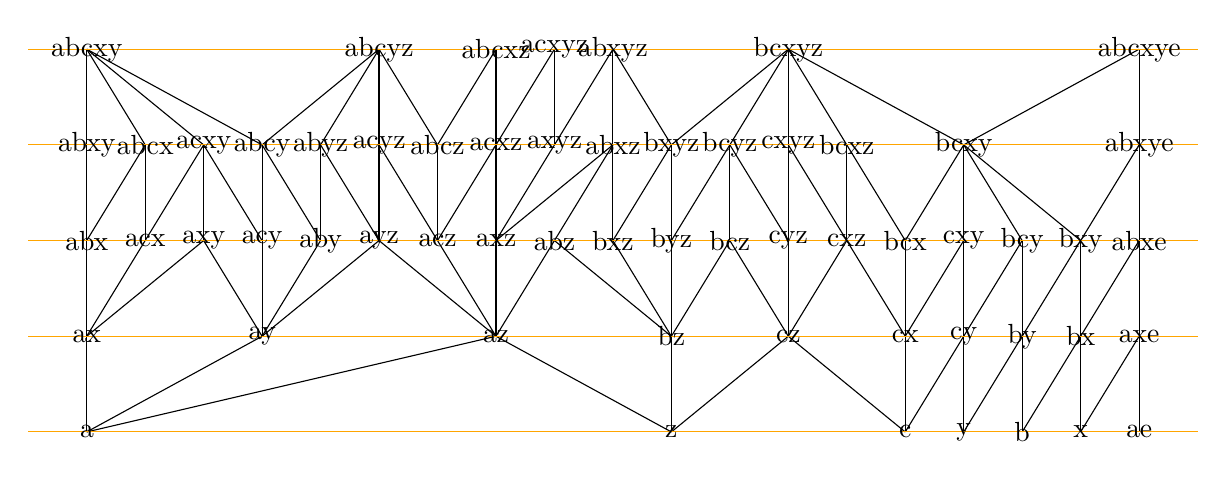
\begin{tikzpicture}[scale = 1.35,yscale = 0.9,xscale = 0.55]

\coordinate (a) at (3,0);
\coordinate (b) at (19,0);
\coordinate (c) at (17,0);
\coordinate (x) at (20,0);
\coordinate (y) at (18,0);
\coordinate (z) at (13,0);
\coordinate (ae) at (21,0);

\coordinate (ax) at (3,1);
\coordinate (ay) at (6,1);
\coordinate (az) at (10,1);
\coordinate (bz) at (13,1);
\coordinate (cz) at (15,1);
\coordinate (cx) at (17,1);
\coordinate (cy) at (18,1);
\coordinate (by) at (19,1);
\coordinate (bx) at (20,1);
\coordinate (axe) at (21,1);

\coordinate (abx) at (3,2);
\coordinate (acx) at (4,2);
\coordinate (axy) at (5,2);
\coordinate (acy) at (6,2);
\coordinate (aby) at (7,2);
\coordinate (ayz) at (8,2);
\coordinate (acz) at (9,2);
\coordinate (axz) at (10,2);
\coordinate (abz) at (11,2);
\coordinate (bxz) at (12,2);
\coordinate (byz) at (13,2);
\coordinate (bcz) at (14,2);
\coordinate (cyz) at (15,2);
\coordinate (cxz) at (16,2);
\coordinate (bcx) at (17,2);
\coordinate (cxy) at (18,2);
\coordinate (bcy) at (19,2);
\coordinate (bxy) at (20,2);
\coordinate (abxe) at (21,2);

\coordinate (abxy) at (3,3);
\coordinate (abcx) at (4,3);
\coordinate (acxy) at (5,3);
\coordinate (abcy) at (6,3);
\coordinate (abyz) at (7,3);
\coordinate (acyz) at (8,3);
\coordinate (abcz) at (9,3);
\coordinate (acxz) at (10,3);
\coordinate (axyz) at (11,3);
\coordinate (abxz) at (12,3);
\coordinate (bxyz) at (13,3);
\coordinate (bcyz) at (14,3);
\coordinate (cxyz) at (15,3);
\coordinate (bcxz) at (16,3);
\coordinate (bcxy) at (18,3);
\coordinate (abxye) at (21,3);

\coordinate (abcxy) at (3,4);
\coordinate (abcyz) at (8,4);
\coordinate (abcxz) at (10,4);
\coordinate (acxyz) at (11,4);
\coordinate (abxyz) at (12,4);
\coordinate (bcxyz) at (15,4);
\coordinate (abcxye) at (21,4);

\foreach \a/\b in {abx/abxy,a/ax,a/ay,a/az,z/az,z/bz,z/cz,c/cz,c/cx,c/cy,y/cy,y/by,b/by,b/bx,x/bx,x/axe,ae/axe,ax/abx,ax/acx,ax/axy,ay/axy,ay/acy,ay/aby, ay/ayz,az/ayz,az/acz,az/axz,az/abz,bz/abz,bz/bxz,bz/byz,bz/bcz,cz/bcz,cz/cyz,cz/cxz,cx/cxz,cx/bcx,cx/cxy,cy/cxy,cy/bcy,by/bcy,by/bxy,bx/bxy,bx/abxe,axe/abxe,abx/abcx,acx/abcx,acx/acxy,axy/acxy,acy/acxy,acy/abcy,aby/abcy,aby/abyz,ayz/abyz,ayz/acyz,acz/acyz,acz/abcz,acz/acxz,axz/acxz,axz/axyz,axz/abxz,abz/abxz,bxz/abxz,bxz/bxyz,byz/bxyz,byz/bcyz,bcz/bcyz,cyz/bcyz,cyz/cxyz,cxz/cxyz,cxz/bcxz,bcx/bcxz,bcx/bcxy,cxy/bcxy,bcy/bcxy,bxy/bcxy,bxy/abxye,abxy/abcxy,abcx/abcxy,acxy/abcxy,abcy/abcxy,abcy/abcyz,abyz/abcyz,acyz/abcyz,abcz/abcyz,abcz/abcxz,acxz/abcxz,acxz/acxyz,axyz/acxyz,axyz/abxyz,abxz/abxyz,bxyz/abxyz,bxyz/bcxyz,bcyz/bcxyz,cxyz/bcxyz,bcxz/bcxyz,bcxy/bcxyz,bcxy/abcxye,abxe/abxye,abxye/abcxye}
{\draw (\a) -- (\b);}

\foreach\y in {0,...,4}{
    \draw[thin,Orange] (2,\y) -- (22,\y);
}

\foreach\n in {a,b,c,x,y,z,ax,ay,az,bx,by,bz,cx,cy,cz,abx,aby,abz,acx,acy,acz,bcx,bcy,bcz,axy,bxy,cxy,axz,bxz,cxz,ayz,byz,cyz,abcx,abcy,abcz,abxy,abxz,abyz,acxy,acxz,acyz,bcxy,bcxz,bcyz,axyz,bxyz,cxyz,abcxy,abcxz,abcyz,abxyz,acxyz,bcxyz,ae,axe,abxe,abxye,abcxye}
%{ \node[draw, fill=white] at (\n) {$\n$}; }
{
    \node at (\n) {\bound};
    \node at (\n) {\tube{\n}};
}


\end{tikzpicture}
}
	\caption{The rhombic strip of the poset of connected induced subgraphs of $K_{3,3}$ from \Cref{fig:K33 on sphere} on the plane. The leftmost and rightmost chains are the same, indicating the wraparound. Also note that the empty set and the full graph were omitted for visibility. The ranks are indicated by orange lines as in \Cref{fig:K33 on sphere}.}
	\label{fig:K33 on plane}
\end{figure}

\paragraph{Graph Associahedra}
In \cite{facethamiltonicity}, the authors consider facet-Hamiltonian paths and cycles on graph associahedra. They construct facet-Hamiltonian paths and cycles for graph associahedra of paths, cycles, fans, wheels, complete split graphs and complete graphs. As mentioned in the preliminaries, many of these polytopes are known in different contexts and are very well studied. The two most prominent are the graph associahedron of the path, which is the \defn{classical associahedron}, and the graph associahedron of the complete graph, which is the permutahedron \cite{Associahedron, Associahedra_spines, Associahedra_diameter, Associahedron_realizations, Associahedron_non_leaving_face}. The $(n-3)$-dimensional classical associahedron is the polytope with the following face lattice. Consider the convex $n$-gon in the plane and the set of its diagonals. Two diagonals are compatible if they do not cross. The non-empty faces correspond to sets of pairwise compatible diagonals, ordered by reverse inclusion; adjoining the empty face gives the face lattice. The vertices of the classical associahedron are then the triangulations of the convex $n$-gon, a Catalan family. Using any Catalan bijection, we may interpret the associahedron via any other Catalan family, such as binary trees or valid bracketings. The latter makes the connection to the graph associahedron of a path clear.

Of special interest are facet-Hamiltonian paths and cycles which consist only of nested tubings. Such nested tubings are associated to permutations of the vertices of the graph, such that every prefix induces a connected subgraph. Hence, the natural poset to consider is the poset of tubes of a connected graph, ordered by inclusion and with $\emptyset$ and $V(G)$ adjoined. Then the flags of this poset are exactly the nested tubings of the graph, and a rhombic strip will correspond to a facet-Hamiltonian path or cycle in which all tubings are nested. The facet-Hamiltonian cycles defined in \cite{facethamiltonicity} for cycles, complete split graphs and complete graphs are of this nature. Furthermore, the facet-Hamiltonian path in the case where the graph is a path is also of this nature. Hence, these constructions give rise to rhombic strips.

\paragraph{Graph associahedra of trees}
In \cite{facethamiltonicity}, the authors also consider graph associahedra of caterpillars, and establish facet-Hamiltonian paths for them. Using rhombic strips, we are able to construct facet-Hamiltonian paths and cycles for graph associahedra of all trees, deeply extending this result. The corresponding poset is the set of rooted subtrees of a rooted base tree, ordered by inclusion of their vertex sets. After removing the empty subtree, this poset is the Cartesian product of the posets for the principal subtrees at the root. Using a combination of unfolding and zigzagging, we are able to construct rhombic strips for these posets. More generally, we show that, if $P$ admits a Hamiltonian rhombic strip and $Q$ admits a non-cyclic rhombic strip, then $P\times Q$ admits a rhombic strip, see \Cref{sec:results} for more details. This rhombic strip then induces part of a facet-Hamiltonian cycle for the graph associahedron of the base tree. Specifically, the corresponding path visits those facets whose tubes contain the root of the base tree. We then flip the tubes down to obtain nested tubings for the subtrees and proceed recursively, see \Cref{fig:tree flipping down} and \Cref{fig:fh for complete binary} for illustrations of the construction. \Cref{fig:8 node tree rs,fig:10 node tree rs,fig:complete binary tree rs} show examples of the constructed rhombic strips. See also \cite{Broom_associahedra_diameter, Tree_associahedra_diameter}, where the authors give good bounds for the diameter of graph associahedra of brooms and trees more generally.

\paragraph{Rhombic strips for Catalan families}
The rhombic strip of rooted subtrees of a base tree $T$ from the last paragraph is also of independent interest for many specific trees. For example, let $T$ be a large complete binary tree of depth $d$. Then all binary trees of depth $\le d$ are rooted subtrees of $T$. The set of binary trees with a fixed number $k$ of vertices is a Catalan family. A flip in a tubing corresponds to moving a leaf of a subtree to a new parent. Hence, the bottom ranks (up to rank $d$) of a rhombic strip for the poset of rooted subtrees of $T$ are Gray codes for binary trees with this flip operation, all constructed simultaneously and compatibly with each other via the rhombic strip. This rhombic strip also turns out to be Hamiltonian. This yields a Hamilton path in the following flip graph: Take the set of binary trees with at most $d$ vertices. Connect any pair which differs in adding or removing a leaf. Also connect binary trees with $d$ vertices which differ in moving a leaf to a new parent.

When $T$ is a star with $n$ leaves and the center as root, any subset of its leaves together with the root induces a subtree. Hence, the non-empty rooted subtrees form $\mathcal B_n$. If $T$ consists of a root with $n$ paths of lengths $b_1,\ldots,b_n$ attached, its non-empty rooted subtrees form $C_{b_1}\times\ldots\times C_{b_n}$. In both cases, $P_r(T)$ has one additional minimum, the empty subtree.

\paragraph{Venn diagrams}
\begin{figure}
	\centering
	

\begin{tikzpicture}[scale=.6, every node/.style={font=\scriptsize}]
\coordinate (12) at (2,2);
\coordinate (23) at (4,2);
\coordinate (13) at (6,2);
\coordinate (34) at (8,2);
\coordinate (24) at (10,2);
\coordinate (14) at (12,2);

\coordinate (1) at (2,0);
\coordinate (2) at (4,0);
\coordinate (3) at (6,0);
\coordinate (4) at (10,0);

\coordinate (123) at (4,4);
\coordinate (134) at (8,4);
\coordinate (234) at (10,4);
\coordinate (124) at (12,4);

\foreach \a/\b in {1/12,2/12,2/23,3/23,3/13,3/34,4/34,4/24,4/14,12/123,23/123,13/123,13/134,34/134,34/234,24/234,24/124,14/124}
{  \draw (\a) -- (\b);  }

\foreach\n in {1,2,3,4,12,13,14,23,24,34,123,124,134,234}
{ \node[draw, fill = white] at (\n) {$\n$}; }

%1
\draw [thick, Vermilion] plot [smooth] coordinates {(1,-1) (2.4,-.8) (3,2.8) (4.7,2.8) (5.3,1) (6,1) (7,2) (10,5) (11,3) (11.5,1) (13.5,-1)};

%2
\draw [thick, Blue] plot [smooth] coordinates {(1,1) (2.5,1) (3.5,-1) (4.5,-1) (5.5,3) (7,5) (8.5,5) (9,2) (10,1) (12,3) (12.5,2.8) (13.5,1)};

%3
\draw [thick, Green] plot [smooth] coordinates {(1,3) (2.5,3) (4,1) (5,0) (6,-1) (10,3) (12,5) (13.5,3)};

%4
\draw [thick, Purple] plot [smooth] coordinates {(1,5) (5,5) (8,1) (10,-1) (13,2) (13.3,4.5) (13.5,5)};

\end{tikzpicture}
	\caption{A rhombic strip of $\mathcal B_4$ and the corresponding Venn diagram. Each curve of the Venn diagram includes all subsets containing a certain number above it. Orange: 1, Blue: 2, Green: 3, Purple: 4.}
	\label{fig:Boolean4 venn}
\end{figure}
The dual of a cyclic rhombic strip of $\mathcal B_n$ has the subsets of $[n]$ as its faces. In fact, one can decompose the edges of the dual into cycles and hence identify these duals as Venn diagrams: Let the edges of the dual which separate a subset containing $i$ from one not containing it be collected into $\phi_i$. It is easy to see that the edges in $\phi_i$ span a cycle for $i=1,\ldots,n$. The set of simple monotone Venn diagrams is in bijection to the set of cyclic rhombic strips of $\mathcal B_n$ via this duality. \defn{Simple} means that no three cycles of a Venn diagram intersect in a common point and \defn{monotone} means that its cycles can be drawn on the sphere to be $c$-monotone.

\paragraph{Gray codes for multisets}
\begin{figure}[htbp]
	\centering
	% Subfigure 1
	\begin{subfigure}[b]{0.48\textwidth}
		\centering
		
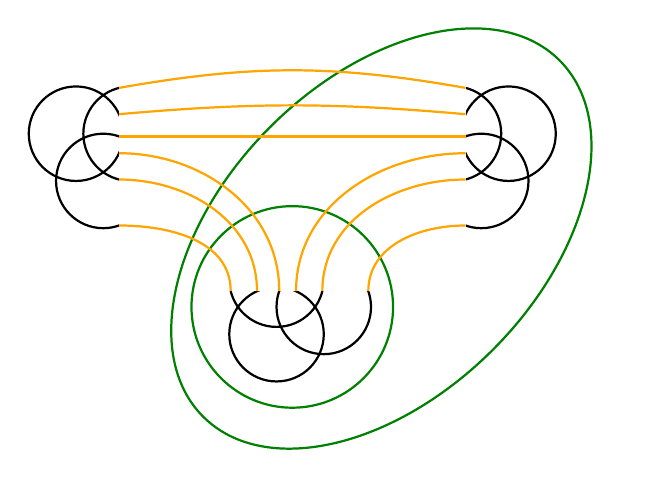
\begin{tikzpicture}[scale=.4]

    % Define the base 3-circle Venn diagram as a reusable macro
    \def\venndiagram{
        \draw[thick] (-90:1) circle (1.5);
        \draw[thick] (30:1) circle (1.5);
        \draw[thick] (150:1) circle (1.5);
    }

    % Define the exact symmetric cut points at x = 0.5 
    % Ordered from top to bottom
    \def\cutX{0.5}
    \def\yA{1.9546} % C2 Top
    \def\yB{1.1197} % C3 Top
    \def\yC{0.4142} % C1 Top
    \def\yD{-0.1197} % C3 Bottom
    \def\yE{-0.9546} % C2 Bottom
    \def\yF{-2.4142} % C1 Bottom

    % --- LEFT DIAGRAM ---
    % Cut on the right side, strands point RIGHT
    \begin{scope}[xshift=-6cm, yshift=0cm]
        \venndiagram
        \fill[white] (\cutX, -3) rectangle (3, 3);
        
        \coordinate (L1) at (\cutX, \yA);
        \coordinate (L2) at (\cutX, \yB);
        \coordinate (L3) at (\cutX, \yC);
        \coordinate (L4) at (\cutX, \yD);
        \coordinate (L5) at (\cutX, \yE);
        \coordinate (L6) at (\cutX, \yF);
    \end{scope}

    % --- RIGHT DIAGRAM ---
    % Mirrored, cut on the left side, strands point LEFT
    \begin{scope}[xshift=6cm, yshift=0cm, xscale=-1]
        \venndiagram
        \fill[white] (\cutX, -3) rectangle (3, 3);
        
        \coordinate (R1) at (\cutX, \yA);
        \coordinate (R2) at (\cutX, \yB);
        \coordinate (R3) at (\cutX, \yC);
        \coordinate (R4) at (\cutX, \yD);
        \coordinate (R5) at (\cutX, \yE);
        \coordinate (R6) at (\cutX, \yF);
    \end{scope}

    % --- MIDDLE DIAGRAM ---
    % Shifted down and rotated 90 degrees.
    % The cut is now on TOP. Strands point UP.
    % Due to rotation mapping (x,y) -> (-y,x), M1 is now the leftmost point, M6 rightmost.
    \begin{scope}[xshift=0cm, yshift=-5cm, rotate=90]
        \venndiagram
        \fill[white] (\cutX, -3) rectangle (3, 3);
        
        \coordinate (M1) at (\cutX, \yA);
        \coordinate (M2) at (\cutX, \yB);
        \coordinate (M3) at (\cutX, \yC);
        \coordinate (M4) at (\cutX, \yD);
        \coordinate (M5) at (\cutX, \yE);
        \coordinate (M6) at (\cutX, \yF);
    \end{scope}

    % --- NEW ENCLOSING CURVE ---
    % Enclosing the middle copy as requested
    \draw[Green, thick] (0, -5) circle (3.2cm);

    \draw[Green, thick, rotate=45] (0,-4) ellipse (8cm and 5cm);


    % --- CONNECTING CURVES ---
    % in/out angles control tangents perfectly to avoid cusps and tangles.

    % 1. Left (Upper) to Right (Upper) - Arching over the top
    \draw[Orange, thick] (L1) to[out=10, in=170] (R1);
    \draw[Orange, thick] (L2) to[out=5,  in=175] (R2);
    \draw[Orange, thick] (L3) to[out=0,  in=180] (R3);

    % 2. Left (Lower) to Middle (Left side)
    % Leaves L pointing Right (out=0), Arrives M from above (in=90)
    % Sorted by width/height so they perfectly nest inside each other
    \draw[Orange, thick] (L4) to[out=0, in=90] (M3);
    \draw[Orange, thick] (L5) to[out=0, in=90] (M2);
    \draw[Orange, thick] (L6) to[out=0, in=90] (M1);

    % 3. Right (Lower) to Middle (Right side)
    % Leaves R pointing Left (out=180), Arrives M from above (in=90)
    \draw[Orange, thick] (R4) to[out=180, in=90] (M4);
    \draw[Orange, thick] (R5) to[out=180, in=90] (M5);
    \draw[Orange, thick] (R6) to[out=180, in=90] (M6);

\end{tikzpicture}
		\caption{Generalized Venn diagram unfolding}
		\label{fig:venn unfolding generalized}
	\end{subfigure}
	\hfill
	% Subfigure 2
	\begin{subfigure}[b]{0.48\textwidth}
		\centering
		
\tikzset{
    triple/.style={
        double,
        double distance=2pt, % Adjust this to change the overall width
    }
}

    \begin{tikzpicture}



\coordinate (mid1) at (-90:1);
\coordinate (mid2) at (30:1);
\coordinate (mid3) at (150:1);

\foreach\x in {1,2,3}
{
    \draw[thick](mid\x) circle (1.5);
}

\coordinate (e) at ($2.5*(mid1) + 2.5*(mid3)$);

\coordinate (1) at ($1.5*(mid1)$);
\coordinate (2) at ($1.5*(mid2)$);
\coordinate (3) at ($1.5*(mid3)$);

\coordinate (12) at ($.9*(mid1) + .9*(mid2)$);
\coordinate (13) at ($.9*(mid1) + .9*(mid3)$);
\coordinate (23) at ($.9*(mid2) + .9*(mid3)$);

\coordinate (123) at (0,0);


\draw[thick, Orange, triple] (1) 
\foreach\x in {12,2,23,123,13,3,e,1}{ -- (\x)};

\foreach\x in {1,2,3,12,13,23,123}
{
    \node[fill=white, draw=gray , inner sep=1.5pt] at (\x) {\scriptsize\x};
}
\node[fill=white, draw=gray, inner sep=1.5pt] at (e) {\scriptsize$\emptyset$};



    \end{tikzpicture}
		\caption{Generalized Venn diagram zigzagging}
		\label{fig:venn zigzagging generalized}
	\end{subfigure}

	\caption{The generalizations of the unfolding and zigzagging constructions for Venn diagrams. (\textsc{a}) Placing multiple copies of the old diagram presents no problems. The curves can be joined in a cycle. When placing $n$ copies, we must add $n-1$ new curves (green) to create a nested structure on the copies. (\textsc{b}) To generalize the zigzagging construction, we may simply place multiple parallel copies of the Hamilton cycle in the dual.}
	\label{fig:combined venn generalized}
\end{figure}

\begin{figure}[ht]
	\centering
	\makebox[\textwidth][c]{\scalebox{0.55}{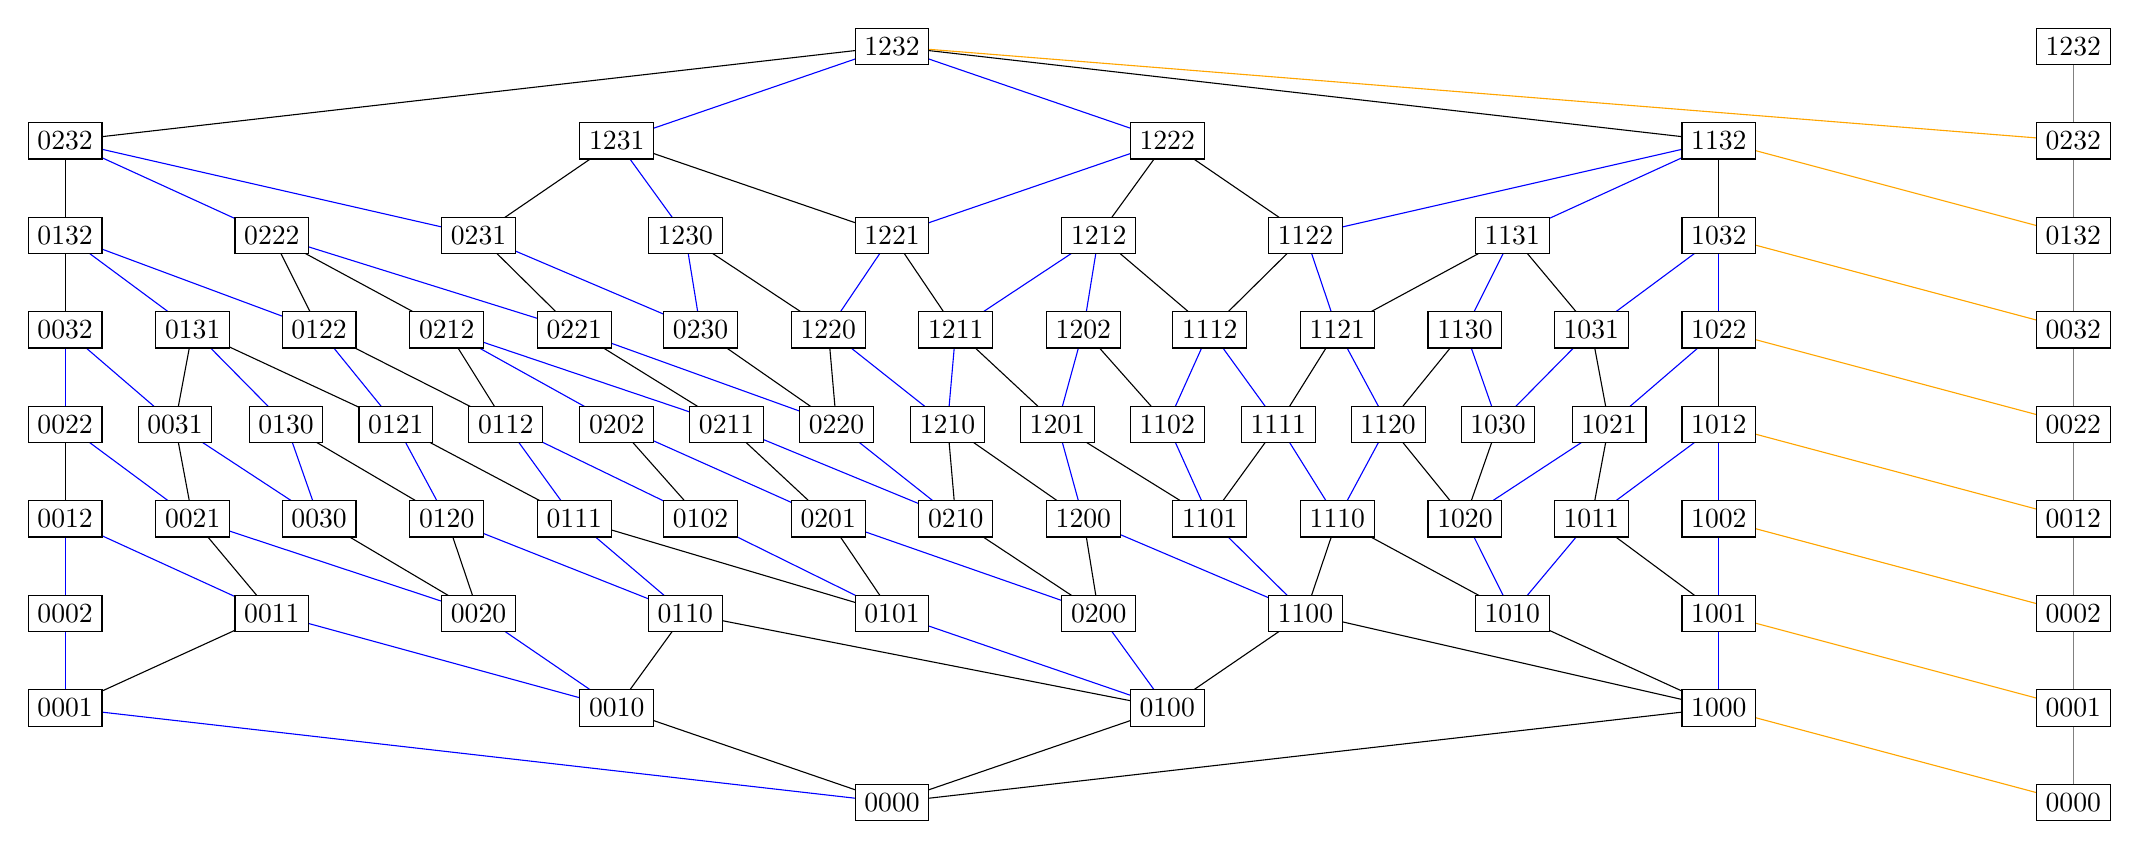
\begin{tikzpicture}[scale=0.6,xscale=2.5,yscale=2]
\newcommand{\edgesaboveclr}{Black}
\newcommand{\edgesbelowclr}{Black}
\newcommand{\edgespathclr}{Blue}
\newcommand{\edgeszipperclr}{Orange}
\coordinate (0000) at (7.00, 0);
\coordinate (0001) at (0.00, 1);
\coordinate (0002) at (0.00, 2);
\coordinate (0012) at (0.00, 3);
\coordinate (0011) at (1.75, 2);
\coordinate (0010) at (4.67, 1);
\coordinate (0020) at (3.50, 2);
\coordinate (0021) at (1.08, 3);
\coordinate (0022) at (0.00, 4);
\coordinate (0032) at (0.00, 5);
\coordinate (0031) at (0.93, 4);
\coordinate (0030) at (2.15, 3);
\coordinate (0130) at (1.87, 4);
\coordinate (0131) at (1.08, 5);
\coordinate (0132) at (0.00, 6);
\coordinate (0122) at (2.15, 5);
\coordinate (0121) at (2.80, 4);
\coordinate (0120) at (3.23, 3);
\coordinate (0110) at (5.25, 2);
\coordinate (0111) at (4.31, 3);
\coordinate (0112) at (3.73, 4);
\coordinate (0102) at (5.38, 3);
\coordinate (0101) at (7.00, 2);
\coordinate (0100) at (9.33, 1);
\coordinate (0200) at (8.75, 2);
\coordinate (0201) at (6.46, 3);
\coordinate (0202) at (4.67, 4);
\coordinate (0212) at (3.23, 5);
\coordinate (0211) at (5.60, 4);
\coordinate (0210) at (7.54, 3);
\coordinate (0220) at (6.53, 4);
\coordinate (0221) at (4.31, 5);
\coordinate (0222) at (1.75, 6);
\coordinate (0232) at (0.00, 7);
\coordinate (0231) at (3.50, 6);
\coordinate (0230) at (5.38, 5);
\coordinate (1230) at (5.25, 6);
\coordinate (1231) at (4.67, 7);
\coordinate (1232) at (7.00, 8);
\coordinate (1222) at (9.33, 7);
\coordinate (1221) at (7.00, 6);
\coordinate (1220) at (6.46, 5);
\coordinate (1210) at (7.47, 4);
\coordinate (1211) at (7.54, 5);
\coordinate (1212) at (8.75, 6);
\coordinate (1202) at (8.62, 5);
\coordinate (1201) at (8.40, 4);
\coordinate (1200) at (8.62, 3);
\coordinate (1100) at (10.50, 2);
\coordinate (1101) at (9.69, 3);
\coordinate (1102) at (9.33, 4);
\coordinate (1112) at (9.69, 5);
\coordinate (1111) at (10.27, 4);
\coordinate (1110) at (10.77, 3);
\coordinate (1120) at (11.20, 4);
\coordinate (1121) at (10.77, 5);
\coordinate (1122) at (10.50, 6);
\coordinate (1132) at (14.00, 7);
\coordinate (1131) at (12.25, 6);
\coordinate (1130) at (11.85, 5);
\coordinate (1030) at (12.13, 4);
\coordinate (1031) at (12.92, 5);
\coordinate (1032) at (14.00, 6);
\coordinate (1022) at (14.00, 5);
\coordinate (1021) at (13.07, 4);
\coordinate (1020) at (11.85, 3);
\coordinate (1010) at (12.25, 2);
\coordinate (1011) at (12.92, 3);
\coordinate (1012) at (14.00, 4);
\coordinate (1002) at (14.00, 3);
\coordinate (1001) at (14.00, 2);
\coordinate (1000) at (14.00, 1);
\coordinate (0000e) at (17, 0);
\coordinate (0001e) at (17, 1);
\coordinate (0002e) at (17, 2);
\coordinate (0012e) at (17, 3);
\coordinate (0022e) at (17, 4);
\coordinate (0032e) at (17, 5);
\coordinate (0132e) at (17, 6);
\coordinate (0232e) at (17, 7);
\coordinate (1232e) at (17, 8);
\foreach\a/\b in {
0112/0212, 0122/0222, 0132/0232, 1212/1112, 1222/1122, 1232/1132, 0011/0021, 0012/0022, 0031/0131, 0032/0132, 0121/0111, 0122/0112, 0101/0201, 0102/0202, 0211/0221, 0212/0222, 0231/1231, 0232/1232, 1221/1211, 1222/1212, 1201/1101, 1202/1102, 1111/1121, 1112/1122, 1131/1031, 1132/1032, 1021/1011, 1022/1012}{
    \draw[\edgesaboveclr] (\a) -- (\b);
}
\foreach\a/\b in {
0000/1000, 0100/1100, 0000/0100, 0010/0110, 0020/0120, 0200/1200, 0210/1210, 0220/1220, 1100/1000, 1110/1010, 1120/1020, 0000/0010, 0001/0011, 0020/0030, 0021/0031, 0130/0120, 0131/0121, 0110/0100, 0111/0101, 0200/0210, 0201/0211, 0220/0230, 0221/0231, 1230/1220, 1231/1221, 1210/1200, 1211/1201, 1100/1110, 1101/1111, 1120/1130, 1121/1131, 1030/1020, 1031/1021, 1010/1000, 1011/1001}{
    \draw[\edgesbelowclr] (\a) -- (\b);
}
\foreach\a/\b in {
0000/0001, 0001/0002, 0002/0012, 0012/0011, 0011/0010, 0010/0020, 0020/0021, 0021/0022, 0022/0032, 0032/0031, 0031/0030, 0030/0130, 0130/0131, 0131/0132, 0132/0122, 0122/0121, 0121/0120, 0120/0110, 0110/0111, 0111/0112, 0112/0102, 0102/0101, 0101/0100, 0100/0200, 0200/0201, 0201/0202, 0202/0212, 0212/0211, 0211/0210, 0210/0220, 0220/0221, 0221/0222, 0222/0232, 0232/0231, 0231/0230, 0230/1230, 1230/1231, 1231/1232, 1232/1222, 1222/1221, 1221/1220, 1220/1210, 1210/1211, 1211/1212, 1212/1202, 1202/1201, 1201/1200, 1200/1100, 1100/1101, 1101/1102, 1102/1112, 1112/1111, 1111/1110, 1110/1120, 1120/1121, 1121/1122, 1122/1132, 1132/1131, 1131/1130, 1130/1030, 1030/1031, 1031/1032, 1032/1022, 1022/1021, 1021/1020, 1020/1010, 1010/1011, 1011/1012, 1012/1002, 1002/1001, 1001/1000}{
    \draw[\edgespathclr] (\a) -- (\b);
}
\foreach\a/\b in {
1000/0000e, 1001/0001e, 1002/0002e, 1012/0012e, 1022/0022e, 1032/0032e, 1132/0132e, 1232/0232e}{
    \draw[\edgeszipperclr] (\a) -- (\b);
}
\foreach\a/\b in {
0000e/0001e, 0001e/0002e, 0002e/0012e, 0012e/0022e, 0022e/0032e, 0032e/0132e, 0132e/0232e, 0232e/1232e}{
    \draw[gray] (\a) -- (\b);
}
\foreach\v in {
0000, 0001, 0002, 0012, 0011, 0010, 0020, 0021, 0022, 0032, 0031, 0030, 0130, 0131, 0132, 0122, 0121, 0120, 0110, 0111, 0112, 0102, 0101, 0100, 0200, 0201, 0202, 0212, 0211, 0210, 0220, 0221, 0222, 0232, 0231, 0230, 1230, 1231, 1232, 1222, 1221, 1220, 1210, 1211, 1212, 1202, 1201, 1200, 1100, 1101, 1102, 1112, 1111, 1110, 1120, 1121, 1122, 1132, 1131, 1130, 1030, 1031, 1032, 1022, 1021, 1020, 1010, 1011, 1012, 1002, 1001, 1000}{
    \node[draw,fill=white] at (\v) {\v};
}
\foreach\v in {
0000, 0001, 0002, 0012, 0022, 0032, 0132, 0232, 1232}{
    \node[draw,fill=white] at (\v e) {\v};
}
\end{tikzpicture}}}
	\caption{A rhombic strip for the grid with dimensions $(2,3,4,3)$. The edges wrapping around are drawn in orange. The $c$-monotone Hamilton path is drawn in blue.}
	\label{fig:multiset small}
\end{figure}
In 1996, Ruskey and Savage \cite{Combinations_multi_set} constructed a Gray code for the combinations of a \defn{multiset}. Let $M=\{1^{(b_1)},2^{(b_2)},\ldots,n^{(b_n)}\}$ denote the multiset which contains the number $i$ exactly $b_i$ times, for $i\in[n]$ and given integers $b_1,\ldots b_n\in\N$. A $k$-combination of $M$ is then a multi subset $K=\{1^{(a_1)},\ldots,n^{(a_n)}\}$, with $a_i\le b_i$, $i\in[n]$ and $\sum_{i=1}^na_i=k$. In what follows, we will identify a multiset simply by its vector of bounds, i.e. $M\sim (b_1,\ldots,b_n)$ and $K\sim (a_1,\ldots, a_n)$. Ruskey and Savage considered the flip on $k$-combinations which decrements one entry and increments another, while staying within the bounds. In the language of multisets, successive $k$-combinations must have symmetric difference of size 2.
They construct a Gray code of such combinations and conjecture that a cyclic Gray code should exist. Using rhombic strips and the unfolding and zigzagging constructions, we are able to construct rhombic strips for the case where the poset $P$ is a product of chains, $P=C_{b_1}\times\ldots\times C_{b_n}$. If at least one height $b_i$ is odd, then the rhombic strip is cyclic. Note that the elements of $P$ are precisely the subsets of $M=\{1^{(b_1)},\ldots,n^{(b_n)}\}$ under the correspondence with integer combinations. Furthermore, $P$ becomes a graded poset with the rank function $(a_1,\ldots,a_n)\mapsto a_1+\ldots+a_n$. Then the elements of rank $k$ of $P$ correspond to $k$-combinations of $M$. For two adjacent elements $x\ne y$ of rank $k$ of $R$, there must exist elements $x\land y$ and $x\lor y$ of rank $k-1$ and $k+1$, respectively, such that $x,x\land y,y,x\lor y$ form a rhombus of $R$. In this case, $x\land y=x\cap y$ and $x\lor y= x\cup y$, and therefore the symmetric difference of $x$ and $y$ must be of size 2. In other words, $x$ and $y$ are adjacent by the flip described above. Hence, we obtain a (cyclic) Gray code for multiset combinations of $M$. Furthermore, these rhombic strips are Hamiltonian. Hence we obtain Gray codes for the subsets of a multiset $M$ which restrict to Gray codes of the $k$-combinations of $M$.

\paragraph{Venn diagrams for multisets}
$\mathcal B_n$ for subsets of $[n]$ is the product of $n$ chains of length 1, $C_1\times\ldots\times C_1$, and cyclic rhombic strips of it correspond to simple monotone Venn diagrams. Looking at rhombic strips of more general products of chains, one can show that the edges of their dual graphs partition into cycles as well. Hence, we obtain \defn{generalized Venn diagrams}, whose regions are the multi subsets of some given multiset, see \Cref{fig:combined venn generalized}.



\section{Proofs}\label{sec:proofs}

Let $R$ be a rhombic strip and $v$ be any element. Then $R\times\{v\}$ is obtained from $R$ by replacing any vertex $x$ of $R$ by $(x,v)$. Similarly, if $H$ is a path or cycle on $R$, then $H\times\{v\}$ is the induced path or cycle on $R\times\{v\}$.

\subsection{Unfolding}

\begin{figure}[!ht]
	\centering
	
\def\lensangle{40}
\def\xstep{2.5cm}
\def\ystep{1.5cm}
\def\numlines{4}

\newcommand{\lens}[2]{
\begin{scope}[xshift=#1*\xstep, yshift=#2*\ystep]
    \node[circle, fill, inner sep=2pt] (lenstop#1#2) at (0,2) {};
    \node[circle, fill, inner sep=2pt] (lensbottom#1#2) at (0,-2) {};
    
    \filldraw[draw=black,fill=white] 
        (lenstop#1#2.center) to[bend left=\lensangle] (lensbottom#1#2.center) 
        to[bend left=\lensangle] (lenstop#1#2.center) -- cycle;
        
    \pgfmathtruncatemacro\sign{mod(#1,2)}
    \if\sign 0{\draw[-{Latex[length=2.5mm, width=1.5mm]}] (-0.3,0) -- (0.3,0);}\else{\draw[{Latex[length=2.5mm, width=1.5mm]}-] (-0.3,0) -- (0.3,0);}\fi
\end{scope}
}


    \begin{tikzpicture}[scale=0.5]

        \pgfmathsetmacro\linestep{1/\numlines}
    
        \foreach\x/\y in {0/0,1/1,2/2,3/3,4/4,5/5}
        {
            \lens{\x}{\y}
            \node at (lensbottom\x\y) [below=5mm] {\scriptsize $R\times\{\x\}$};
        }
        \begin{scope}[on background layer]
            \foreach \x/\y [
                remember=\x as \oldx (initially 0), 
                remember=\y as \oldy (initially 0)
            ] in {0/0,1/1,2/2,3/3,4/4,5/5}
            {
                \foreach\i in {0,0.25,0.5,0.75,1}
                {
                    \draw ($(lenstop\x\y) !\i! (lensbottom\x\y)$) -- ($(lenstop\oldx\oldy) !\i! (lensbottom\oldx\oldy)$);
                }
            }
        \end{scope}
        
    \end{tikzpicture}
    
	\caption{The unfolding construction. The arrows indicate whether a strip was mirrored or not.}
	\label{fig:unfolding}
\end{figure}

\unfolding*
\begin{proof}
	Let $R$ be a rhombic strip of $P$ with left and right boundaries given by the maximal chains $(\ell_1, \ldots, \ell_n)$ and $(r_1, \ldots, r_n)$, respectively. We construct a rhombic strip for the product $P \times C_b$ by layering and connecting planar embeddings of $R$.

	First, fix a planar, straight-line embedding of $R$ where every element of rank $k$ is assigned a $y$-coordinate of $k$. For each index $i \in \{0, \ldots, b\}$, this induces a planar embedding for the layer $R_i = R \times \{i\}$. We translate each layer $R_i$ such that its minimum is mapped to $(i, i)$, and its maximum is mapped to $(i, n-1+i)$. By applying a sufficiently small horizontal scaling to each $R_i$, we ensure that the bounding boxes of these layers are pairwise disjoint.

	Next, we apply a horizontal reflection across the vertical axis $x=i$ to every layer $R_i$ where $i$ is odd (see \Cref{fig:unfolding}).

	We then insert the following covering edges between adjacent layers. For $i=0,\ldots,b-1$ and each $j \in \{1,\ldots,n\}$:
	\begin{itemize}
		\item If $i$ is even, add the edges connecting $(r_j, i)$ and $(r_j, i+1)$.
		\item If $i$ is odd, add the edges connecting $(\ell_j, i)$ and $(\ell_j, i+1)$.
	\end{itemize}

	Because of the alternating reflections, these edges induce no crossings.

	When $b=1$ and the two boundary chains meet only at 0 and 1, we may add the additional edges connecting $(\ell_j, 0)$ and $(\ell_j, 1)$ for $j = 1, \ldots, n$. These edges can be routed around the back of the sphere. The edges at 0 and 1 are already present. Since the boundary chains have no internal vertex in common, all other added edges are new; together, these edges divide the outer face into rhombi, closing the structure into a cyclic rhombic strip.

	Finally, if $R$ is Hamiltonian, the Hamilton paths of each layer $R_i$ can be concatenated by using the covering edges.
\end{proof}

\subsection{Zigzagging}

\begin{figure}[!ht]
	\centering
	

\def\lensangle{40}
\def\xstep{2.5cm}
\def\ystep{1.5cm}
\def\numlines{4}
\def\scew{5}
\def\height{3}

\newcommand{\lens}[2]{
\begin{scope}[xshift=#1*\xstep, yshift=#2*\ystep]
    
    \filldraw[draw=black,fill=white] 
        (\scew,\height) to[bend left=\lensangle] (-\scew,-\height) 
        to[bend left=\lensangle] (\scew,\height) -- cycle;

        \path (\scew,\height) to[bend left=\lensangle] node[pos=0.5, above] {\scriptsize$R_-$} (-\scew,-\height);
\path (-\scew,-\height) to[bend left=\lensangle] node[pos=0.5, below] {\scriptsize$R^-$} (\scew,\height);

    \node[circle, fill, inner sep=2pt] (lenstop#1#2) at (\scew,\height) {};
    \node[circle, fill, inner sep=2pt] (lensbottom#1#2) at (-\scew,-\height) {};
        
\end{scope}
}
    \begin{tikzpicture}[scale=0.5]

        \lens{0}{0}

        \draw[thick,Orange] 
        (lensbottom00) -- 
        ++(3,3) -- 
        ++(1,-1) -- 
        ++(3,3) --
        ++(1,-1) --
        ++(2,2);
        
        \node[circle, fill, inner sep=2pt] at (lensbottom00) {};

        \draw[-{Latex[length=2.5mm, width=1.5mm]}] (5,0) -- (6,0);

        \node[circle, fill, inner sep=2pt] (bb) at (7,-2-\height) {};
        \node[circle, fill, inner sep=2pt] (bt) at (17,-2+\height) {};
        \node[circle, fill, inner sep=2pt] (tb) at (7,+2-\height) {};
        \node[circle, fill, inner sep=2pt] (tt) at (17,+2+\height) {};

        \draw (bb) to[bend right=\lensangle] (bt);
        \draw (tb) to[bend left=\lensangle] (tt);
        \draw (bb) -- (tb) (bt) -- (tt);
        \path (bb) to[bend right=\lensangle] node[pos=0.5, above] {\scriptsize$R_-\times\{0\}$} (bt);
        \path (tb) to[bend left=\lensangle] node[pos=0.5, below] {\scriptsize$R^-\times\{b\}$} (tt);

        \draw[thick,Orange] 
        (bb) -- 
        ++(3,3) -- 
        ++(1,-1) -- 
        ++(3,3) --
        ++(1,-1) --
        ++(2,2);
        
        \draw[thick,Orange] 
        (tb) -- 
        ++(3,3) -- 
        ++(1,-1) -- 
        ++(3,3) --
        ++(1,-1) --
        ++(2,2);

        \draw 
        (bb) 
        ++(1,1) -- +(0,4)
        ++(1,1) -- +(0,4)
        ++(1,1) -- +(0,4)
        ++(1,-1) -- +(0,4)
        ++(1,1) -- +(0,4)
        ++(1,1) -- +(0,4)
        ++(1,1) -- +(0,4)
        ++(1,-1) -- +(0,4)
        ++(1,1) -- +(0,4);

        \draw
        (bb) ++(0,1) -- 
        ++(3,3) -- 
        ++(1,-1) -- 
        ++(3,3) --
        ++(1,-1) --
        ++(2,2);
        \draw
        (bb) ++(0,2) -- 
        ++(3,3) -- 
        ++(1,-1) -- 
        ++(3,3) --
        ++(1,-1) --
        ++(2,2);
        \draw
        (bb) ++(0,3) -- 
        ++(3,3) -- 
        ++(1,-1) -- 
        ++(3,3) --
        ++(1,-1) --
        ++(2,2);

        \draw[thick, Blue] (bb) -- ++(0,4) -- ++(1,1) -- ++(0,-4) -- ++(1,1) -- ++(0,4) -- ++(1,1) -- ++(0,-4) -- ++(1,-1) -- ++(0,4) -- ++(1,1) -- ++(0,-4) -- ++(1,1) -- ++(0,4) -- ++(1,1) -- ++(0,-4) -- ++(1,-1) -- ++(0,4) -- ++(1,1) -- ++(0,-4) -- ++(1,1) -- ++(0,4);

        \node[circle, fill, inner sep=2pt] (bb) at (7,-2-\height) {};
        \node[circle, fill, inner sep=2pt] (bt) at (17,-2+\height) {};
        \node[circle, fill, inner sep=2pt] (tb) at (7,+2-\height) {};
        \node[circle, fill, inner sep=2pt] (tt) at (17,+2+\height) {};
        
    \end{tikzpicture}
	\caption{The zigzagging construction, visualized in the plane for a non-cyclic rhombic strip. In orange, the paths $H\times\{0\}$ and $H\times\{b\}$. The $c$-monotone Hamilton path of the resulting strip is drawn in blue.}
	\label{fig:zigzagging}
\end{figure}

\begin{figure}[!ht]
	\centering
	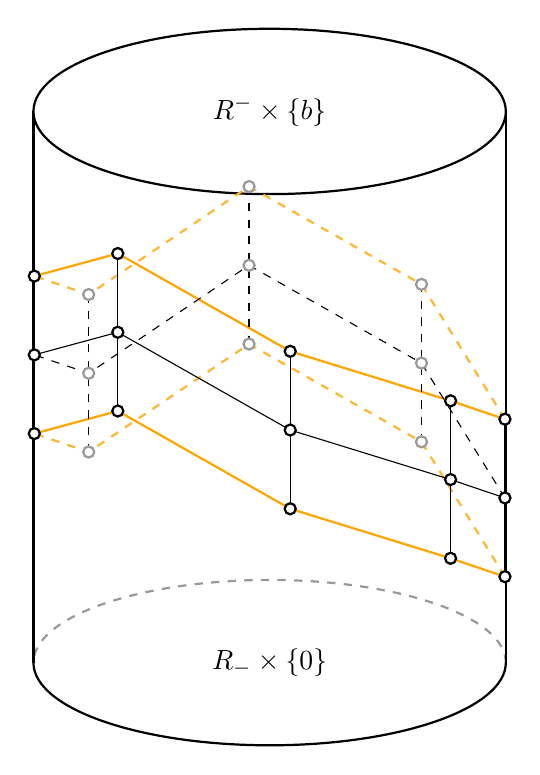
\begin{tikzpicture}[
    x={(1cm, 0cm)},    % x-axis points purely right
    y={(0cm, 0.35cm)}, % y-axis (depth) points up, but is squished for perspective
    z={(0cm, 1cm)}     % z-axis (height) points purely straight up
]

    % --- 1. DEFINE CYLINDER PARAMETERS ---
    \def\R{3} % Radius of the cylinder
    \def\H{2} % Height of the cylinder (z-axis)

    % --- 2. DRAW THE CYLINDER OUTLINE ---
    
    % Bottom base: Back half (hidden, dashed)
    \begin{scope}[canvas is xy plane at z=-1]
        \draw[dashed, color=gray!80, thick] (\R,0) arc (0:180:\R);
        
        % Bottom base: Front half (visible, solid)
        \draw[thick] (\R,0) arc (0:-180:\R);
        \node at (0,0) {$R_-\times\{0\}$};
    \end{scope}

    % Vertical side edges
    \draw[thick] (-\R, 0, -1) -- (-\R, 0, \H+4);
    \draw[thick] (\R, 0, -1) -- (\R, 0, \H+4);

    % Top base (fully visible)
    \begin{scope}[canvas is xy plane at z=\H+4]
        \draw[thick, fill=white, fill opacity=0.7] (0,0) circle[radius=\R];
        \node at (0,0) {$R^-\times\{b\}$};
    \end{scope}
    
    % --- 3. CALCULATE AND DEFINE VERTICES ---
    % Loop through index, angle, and height offset
    % Angles span 0 to 315 degrees (8 points)
    \foreach \i/\a/\h in {
        0/0/0,
        1/45/1,
        2/90/2,
        3/135/1,
        4/180/2,
        5/225/3,
        6/270/2,
        7/315/1
    } {
        % Bottom vertices (B0 to B7)
        \coordinate (B\i) at (xyz cylindrical cs: radius=\R, angle=\a+5, z=\h);
        
        % Top vertices (T0 to T7) - offset by \H
        \coordinate (T\i) at (xyz cylindrical cs: radius=\R, angle=\a+5, z={\H+\h});
        
        \coordinate (M\i) at (xyz cylindrical cs: radius=\R, angle=\a+5, z={\H/2+\h});
    }

    \foreach\L in {T,B}{
        \draw[dashed, color=Orange!80, thick] (\L0) -- (\L1) -- (\L2) -- (\L3) -- (\L4);
        \draw[thick, Orange] (\L4) -- (\L5) -- (\L6) -- (\L7) -- (\L0);
    }
\def\L{M}
    \draw[dashed] (\L0) -- (\L1) -- (\L2) -- (\L3) -- (\L4);
    \draw[] (\L4) -- (\L5) -- (\L6) -- (\L7) -- (\L0);


   

    \foreach\i in {1,2,3}{
        \draw[dashed] (B\i) -- (T\i);
    }
    \foreach\i in {0,4,5,6,7}{
        \draw (B\i) -- (T\i);
    }




     \foreach\L in {T,M,B}{
    \foreach \i in {1,2,3} {
        \filldraw[fill=white, draw=gray!80, thick] (\L\i) circle (2pt);
    }
    \foreach \i in {0,4,5,6,7} {
        \filldraw[fill=white, draw=black, thick] (\L\i) circle (2pt);
    }}
\end{tikzpicture}
	\caption{The zigzagging construction can construct cyclic strips, if the input strip is cyclic. The picture is drawn on the cylinder to avoid distortions.}
	\label{fig:cylinder}
\end{figure}

\zigzagging*
\begin{proof}
	Let $R$ be a (cyclic) rhombic strip of $P$ with a $c$-monotone Hamilton path (or cycle) $H=(v_1, \ldots, v_m)$. The embedding of $H$ partitions the edges of $R$ into three disjoint sets: the edges belonging to $H$, the set of edges $E(R_-)$ located strictly below $H$, and the set of edges $E(R^-)$ located strictly above $H$.

	First, consider the non-cyclic case. Place the vertices of $P\times C_b$ in the plane such that each vertex $(v_i,j)$ is assigned coordinates $(i, \text{rank}(v_i)+j)$. Next, add the edges of $R_-\times\{0\}$, $R^-\times\{b\}$, and $H\times\{i\}$ for $i=0,\ldots,b$.

	Next, we add the edges corresponding to the edges of the chain $C_b$. They are $(v_i,j)-(v_i,j+1)$, for $i=1,\ldots,m$ and $j=0,\ldots,b-1$. The result is a rhombic strip. To obtain a $c$-monotone Hamilton path for this new strip, we zigzag through these last added edges. More precisely, the Hamilton path consists of the edges $(v_i,0)-(v_{i+1},0)$ for $i$ odd and $(v_i,b)-(v_{i+1},b)$ for $i$ even, as well as the edges $(v_i,j)-(v_i,j+1)$, for $i=1,\ldots,m$ and $j=0,\ldots,b-1$, see \Cref{fig:zigzagging}.

	For the cyclic case, the construction proceeds analogously, see \Cref{fig:cylinder}. Because $R$ is a bipartite graph containing a Hamilton cycle, $P$ must have an even number of vertices $m$. This parity condition ensures that the zigzagging path through the copies of $C_b$ aligns correctly at the ends, closing a continuous $c$-monotone Hamilton cycle.
\end{proof}

\subsection{Multiset Combinations}
\begin{figure}
	\centering
	
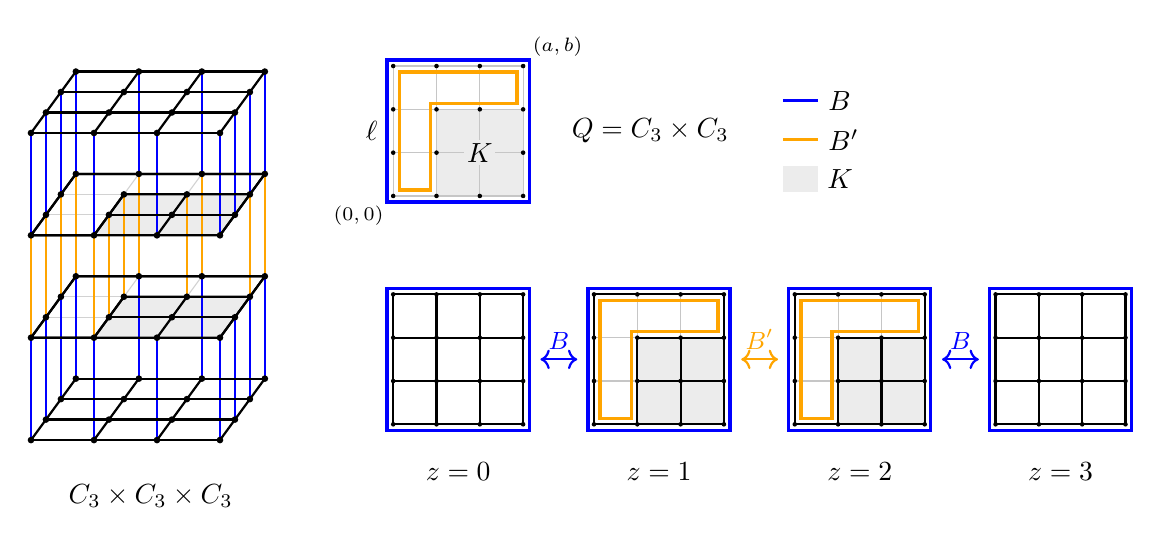
\begin{tikzpicture}
% Q = C_b x C_c with elements (y,z); K = [1,b] x [0,c-1]; layers x = 0,...,a
\def\bb{3}\def\cc{3}\def\aa{3}
\pgfmathtruncatemacro\bm{\bb-1}\pgfmathtruncatemacro\cm{\cc-1}\pgfmathtruncatemacro\am{\aa-1}
\def\off{0.14}% offset of the cycles B (outside) and B' (inside, away from K)

% all commands draw in grid coordinates (y,z) of the current scope
\newcommand{\Qedges}[1]{% all cover relations of Q
  \foreach \y in {1,...,\bb} \foreach \z in {0,...,\cc} \draw[#1] (\y-1,\z) -- (\y,\z);
  \foreach \y in {0,...,\bb} \foreach \z in {1,...,\cc} \draw[#1] (\y,\z-1) -- (\y,\z);}
\newcommand{\Kedges}[1]{% all cover relations of K
  \foreach \y in {1,...,\bm} \foreach \z in {0,...,\cm} \draw[#1] (\y,\z) -- (\y+1,\z);
  \foreach \y in {1,...,\bb} \foreach \z in {1,...,\cm} \draw[#1] (\y,\z-1) -- (\y,\z);}
\newcommand{\cycleA}[1]{\draw[#1] (0,0) -- (\bb,0) -- (\bb,\cc) -- (0,\cc) -- cycle;}
\newcommand{\cycleB}[1]{\draw[#1] (0,0) -- (1,0) -- (1,\cm) -- (\bb,\cm) -- (\bb,\cc) -- (0,\cc) -- cycle;}
% the cycles drawn next to the grid lines: B slightly outside, B' slightly inside
\newcommand{\haloA}{\draw[Blue,line width=1.2pt] (-\off,-\off) rectangle (\bb+\off,\cc+\off);}
\newcommand{\haloB}{\draw[Orange,line width=1.2pt] (\off,\off) -- (1-\off,\off) -- (1-\off,\cm+\off)
  -- (\bb-\off,\cm+\off) -- (\bb-\off,\cc-\off) -- (\off,\cc-\off) -- cycle;}
\newcommand{\shadeK}{\fill[gray!15] (1,0) -- (\bb,0) -- (\bb,\cm) -- (1,\cm) -- cycle;}
\newcommand{\vertices}[1]{\foreach \y in {0,...,\bb} \foreach \z in {0,...,\cc} \fill (\y,\z) circle (#1);}
% vertical edges from the current layer to the next one, along B resp. B'
\newcommand{\vertA}[1]{
  \foreach \y in {0,...,\bb} {\draw[#1] (\y,0) -- ++(0,0,1); \draw[#1] (\y,\cc) -- ++(0,0,1);}
  \foreach \z in {1,...,\cm} {\draw[#1] (0,\z) -- ++(0,0,1); \draw[#1] (\bb,\z) -- ++(0,0,1);}}
\newcommand{\vertB}[1]{
  \foreach \z in {0,...,\cc} \draw[#1] (0,\z) -- ++(0,0,1);
  \foreach \y in {1,...,\bb} \draw[#1] (\y,\cc) -- ++(0,0,1);
  \foreach \z in {0,...,\cm} \draw[#1] (1,\z) -- ++(0,0,1);
  \foreach \y in {2,...,\bb} \draw[#1] (\y,\cm) -- ++(0,0,1);}

%%%%%%%%%%%%%%%%%%%%%%%%%%%%%%%%%%%%%%%%%%%%%%%%%%%%
% Left: the strip in 3d, layers stacked, slightly rotated
%%%%%%%%%%%%%%%%%%%%%%%%%%%%%%%%%%%%%%%%%%%%%%%%%%%%
\begin{scope}[x={(0.8cm,0cm)},y={(0.19cm,0.26cm)},z={(0cm,1.3cm)}]
  \foreach \X in {1,...,\am} {\begin{scope}[shift={(0,0,\X)}] \shadeK \Qedges{gray!35} \end{scope}}
  \foreach \X in {0,...,\am} {\begin{scope}[shift={(0,0,\X)}]
    \pgfmathtruncatemacro\odd{mod(\X,2)}
    \ifnum\odd=0 \vertA{Blue,thick} \else \vertB{Orange,thick} \fi
  \end{scope}}
  \foreach \X in {0,...,\aa} {\begin{scope}[shift={(0,0,\X)}]
    \ifnum\X=0 \Qedges{thick} \else\ifnum\X=\aa \Qedges{thick} \else
      \cycleA{thick} \cycleB{thick} \Kedges{thick} \fi\fi
    \vertices{1.2pt}
  \end{scope}}
  \node at (1.9,0,-0.55) {$C_3\times C_3\times C_3$};
\end{scope}

%%%%%%%%%%%%%%%%%%%%%%%%%%%%%%%%%%%%%%%%%%%%%%%%%%%%
% Top right: the grid Q with K and the cycles B, B'
%%%%%%%%%%%%%%%%%%%%%%%%%%%%%%%%%%%%%%%%%%%%%%%%%%%%
\begin{scope}[xshift=4.6cm,yshift=3.1cm,scale=0.55]
  \shadeK \Qedges{gray!45} \haloA \haloB \vertices{1.5pt}
  \node at (2,1) [fill=gray!15,inner sep=1pt] {$K$};
  \node[left] at (-\off,1.5) {$\ell$};
  \node[below left] at (0,0) {\scriptsize $(0,0)$};
  \node[above right] at (\bb,\cc) {\scriptsize $(a,b)$};
  \node[right] at (\bb+0.9,1.5) {$Q=C_3\times C_3$};
  \draw[Blue,line width=1.2pt] (\bb+6,2.2) -- ++(0.8,0) node[right,black] {$B$};
  \draw[Orange,line width=1.2pt] (\bb+6,1.3) -- ++(0.8,0) node[right,black] {$B'$};
  \fill[gray!15] (\bb+6,0.1) rectangle ++(0.8,0.6); \node[right] at (\bb+6.8,0.4) {$K$};
\end{scope}

%%%%%%%%%%%%%%%%%%%%%%%%%%%%%%%%%%%%%%%%%%%%%%%%%%%%
% Bottom right: the horizontal edges of each layer
%%%%%%%%%%%%%%%%%%%%%%%%%%%%%%%%%%%%%%%%%%%%%%%%%%%%
\foreach \X in {0,...,\aa}{
  \begin{scope}[xshift=4.6cm+\X*2.55cm,yshift=0.2cm,scale=0.55]
    \ifnum\X=0 \Qedges{thick} \else\ifnum\X=\aa \Qedges{thick} \else
      \shadeK \Qedges{gray!45} \cycleA{thick} \cycleB{thick} \Kedges{thick}
    \fi\fi
    % where the vertical edges attach: towards x-1 and x+1 along one cycle each
    \pgfmathtruncatemacro\odd{mod(\X,2)}
    \ifnum\X<\aa \ifnum\odd=0 \haloA \else \haloB \fi \fi
    \ifnum\X>0 \ifnum\odd=1 \haloA \else \haloB \fi \fi
    \vertices{1.5pt}
    \node at (1.5,-1.1) {$z=\X$};
    % arrow to the next layer, labelled by the cycle along which they are joined
    \ifnum\X<\aa
      \ifnum\odd=0 \def\col{Blue}\def\cyc{B}\else\def\col{Orange}\def\cyc{B'}\fi
      \draw[\col,thick,<->] (\bb+0.4,1.5) -- (\bb+1.25,1.5) node[midway,above] {\small$\cyc$};
    \fi
  \end{scope}}
\end{tikzpicture}

	\caption{The construction of \Cref{lem:cyclic-grid-seed} for $a=b=c=3$. Left: the rhombic strip, with the layers $z=0,\ldots,3$ stacked vertically. Top right: the grid $Q$ with the block $K$ (shaded) and the cycles $B$ (blue, drawn slightly outside) and $B'$ (orange, drawn slightly inside). Bottom right: the horizontal edges of each layer in black; edges not in the strip are light gray. The vertical edges are indicated by the arrows and colored cycles: layers $0$ and $1$ as well as $2$ and $3$ are joined along $B$, layers $1$ and $2$ along $B'$.}
	\label{fig:3dgrid}
\end{figure}
\begin{figure}
	\centering
	
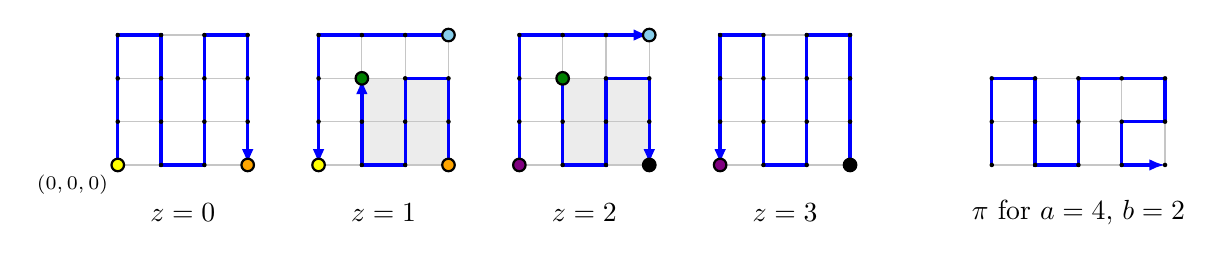
\begin{tikzpicture}
% The Hamilton cycle H of the grid lemma for a = b = c = 3, layer by layer,
% and the path P for even b (b = 4, c = 2).
\def\bb{3}\def\cc{3}\pgfmathtruncatemacro\cm{\cc-1}

\newcommand{\grid}[2]{% light grid of C_#1 x C_#2
  \foreach \y in {1,...,#1} \foreach \z in {0,...,#2} \draw[gray!45] (\y-1,\z) -- (\y,\z);
  \foreach \y in {0,...,#1} \foreach \z in {1,...,#2} \draw[gray!45] (\y,\z-1) -- (\y,\z);}
\newcommand{\vertices}[2]{\foreach \y in {0,...,#1} \foreach \z in {0,...,#2} \fill (\y,\z) circle (1.5pt);}
\newcommand{\shadeK}{\fill[gray!15] (1,0) rectangle (\bb,\cm);}
\tikzset{ham/.style={Blue,very thick,-{Latex[length=2mm]}},
         vert/.style={draw=black,fill=white,thick,circle,inner sep=1.6pt}}
% the pieces of H in grid coordinates
\def\Pfw{(0,0) (0,1) (0,2) (0,3) (1,3) (1,2) (1,1) (1,0) (2,0) (2,1) (2,2) (2,3) (3,3) (3,2) (3,1) (3,0)}
\def\Pbw{(3,0) (3,1) (3,2) (3,3) (2,3) (2,2) (2,1) (2,0) (1,0) (1,1) (1,2) (1,3) (0,3) (0,2) (0,1) (0,0)}
\def\Sfw{(1,2) (1,1) (1,0) (2,0) (2,1) (2,2) (3,2) (3,1) (3,0)}
\def\Sbw{(3,0) (3,1) (3,2) (2,2) (2,1) (2,0) (1,0) (1,1) (1,2)}
\def\Lfw{(0,0) (0,1) (0,2) (0,3) (1,3) (2,3) (3,3)}
\def\Lbw{(3,3) (2,3) (1,3) (0,3) (0,2) (0,1) (0,0)}

\foreach \X/\first/\second/\up/\down in {0/\Pfw//3/0, 1/\Sbw/\Lbw/1/0, 2/\Sfw/\Lfw/3/3, 3/\Pbw///0}{
  \begin{scope}[xshift=\X*2.55cm,scale=0.55]
    \ifnum\X=1 \shadeK\fi \ifnum\X=2 \shadeK\fi
    \grid{\bb}{\cc}
    \draw[ham] plot coordinates {\first};
    \ifx\second\empty\else \draw[ham] plot coordinates {\second}; \fi
    \vertices{\bb}{\cc}
    \node at (1.5,-1.1) {$z=\X$};
  \end{scope}}

% vertices at which H uses a vertical edge; the two ends of each such edge share a color
\newcommand{\vmark}[4]{\node[vert,fill=#4] at ($(#1*2.55cm,0)+0.55*(#2,#3)$) {};}
\vmark{0}{3}{0}{Orange}    \vmark{1}{3}{0}{Orange}     % up at (b,0)
\vmark{1}{1}{2}{Green}     \vmark{2}{1}{2}{Green}      % up at the start of sigma
\vmark{2}{3}{0}{Black} \vmark{3}{3}{0}{Black}  % up at (b,0)
\vmark{3}{0}{0}{Purple}    \vmark{2}{0}{0}{Purple}     % down at (0,0)
\vmark{2}{3}{3}{SkyBlue}   \vmark{1}{3}{3}{SkyBlue}    % down at (b,c)
\vmark{1}{0}{0}{Yellow}    \vmark{0}{0}{0}{Yellow}     % down at (0,0)
\node[below left] at (0,0) {\scriptsize $(0,0,0)$};

% P for even b: zigzag through columns 0,...,b-2, then the last two columns row by row
\begin{scope}[xshift=11.1cm,scale=0.55]
  \grid{4}{2}
  \draw[ham] plot coordinates {(0,0) (0,1) (0,2) (1,2) (1,1) (1,0) (2,0) (2,1) (2,2)
    (3,2) (4,2) (4,1) (3,1) (3,0) (4,0)};
  \vertices{4}{2}
  \node at (2,-1.1) {$\pi$ for $a=4$, $b=2$};
\end{scope}
\end{tikzpicture}

	\caption{The Hamilton cycle $H$ from the proof of \Cref{lem:cyclic-grid-seed} for $a=b=c=3$, drawn layer by layer in blue; $K$ is shaded in the middle layers. $H$ starts in $(0,0,0)$, follows $\pi$ in layer $0$, $\sigma$ backwards and forwards in layers $1$ and $2$, and $\pi$ backwards in layer $3$. It then descends along $\ell$ in layers $2$ and $1$. Circled vertices of the same color are the two ends of a vertical edge of $H$. Right: the path $\pi$ for even $a$, here $a=4$ and $b=2$.}
	\label{fig:3dgrid ham}
\end{figure}
We will obtain cyclic Gray codes for multiset combinations in two steps. First, we consider the case in which one element appears in the multiset an odd number of times. In this case, the following lemma constructs a cyclic rhombic strip for the corresponding product of chains. If all elements appear an even number of times, no cyclic rhombic strip exists, as the following remark shows. However, we can still construct so called mountain range representations for these grids, which establish the missing cases. In both cases, the induction start (3-dimensional grids) is the hardest part.

\begin{remark}\label{rem:grid-parity}
	A product of chains which admits a cyclic rhombic strip has an even number of elements. Indeed, sweeping a maximal chain around the strip gives a cyclic sequence of multiset permutations, with one adjacent transposition of distinct letters for each rhombus. Each transposition changes inversion parity, so the number $F$ of rhombi is even. Since the strip is a quadrangulation, its number of edges is $E=2F$, and Euler's formula gives $V=E-F+2=F+2$, which is even as well. In particular, $C_{b_1}\times\ldots\times C_{b_n}$ has no cyclic rhombic strip when all $b_i$ are even.
\end{remark}
\begin{lemma}[Cyclic rhombic strips for grids]
	\label{lem:cyclic-grid-seed}
	Let $a,b,c \geq 1$ with $c$ odd. Then $C_a \times C_b \times C_c$ admits a
	cyclic Hamiltonian rhombic strip.
\end{lemma}

\begin{proof}
	By symmetry we may assume that $a$ is odd or $b$ is even. Let $Q=C_a\times C_b$, drawn as a planar grid with elements $(x,y)$. We view $Q\times C_c$ as a stack of the layers $Q\times\{z\}$, $z=0,\ldots,c$, and write its elements as $(x,y,z)$. Define the block $K=\{(x,y)\mid x\ge 1,\ y\le b-1\}\cong C_{a-1}\times C_{b-1}$ in the bottom right corner of $Q$. Let $B$ be the outer boundary cycle of $Q$. Let $B'$ be the cycle obtained by flipping $B$ across $K$, i.e. walking the left and top boundary of $K$ instead of the bottom and right, see \Cref{fig:3dgrid}. If $a=1$ or $b=1$, then $B=B'$. The strip $R$ consists of the following edges.
	\begin{itemize}
		\item \emph{Horizontal edges.} In the bottom layer $z=0$ and the top layer $z=c$, all edges of $Q$. In every middle layer $0<z<c$, the edges of $B$ and all edges of $K$.
		\item \emph{Vertical edges.} For $0\le z<c$, the edges $(q,z)-(q,z+1)$ for all $q$ on $B$ if $z$ is even, and for all $q$ on $B'$ if $z$ is odd.
	\end{itemize}

	It is easy to check that $R$ is a rectangulation and every vertex other than $(0,0,0)$ and $(a,b,c)$ has a lower and an upper neighbor. Moreover, around every vertex other than the poles the lower and the upper neighbors form two contiguous blocks: if $s(v)$ counts the changes between lower and upper neighbors around $v$, then, as all faces are rhombi, Euler's formula gives $\sum_v(s(v)-2)=-4$; the poles already contribute $-4$, so $s(v)=2$ for all other vertices. Hence $R$ can be drawn with the elements of rank $k$ on the circle of latitude $k$, and $R$ is a cyclic rhombic strip.

	For the Hamilton cycle, let $\pi$ be the path through $Q$ from $(0,0)$ to $(a,0)$ that zigzags through the columns: up column $0$, down column
	$1$, and so on. For odd $a$ this ends in $(a,0)$. For even $a$ (and hence even $b$), $\pi$ zigzags through the columns $0,\ldots,a-2$ and then
	through the last two columns row by row from the top, which also ends in $(a,0)$. Similarly, let $\sigma$ be the path that zigzags through the
	columns of $K$, starting on the left boundary of $K$ and ending in $(a,0)$. Finally, let $\ell$ be the path from $(0,0)$ to $(a,b)$ along the left
	and top boundary of $Q$; its elements are exactly the elements of $Q$ not in $K$.

	The Hamilton cycle $H$ starts in $(0,0,0)$ and follows $\pi$ along horizontal edges of the bottom layer, see \Cref{fig:3dgrid ham}. In each middle layer it follows $\sigma$, backwards in odd and forwards in even layers, and it moves up to the next layer along the vertical edge at $(a,0)$, which lies on $B$, or at the start of $\sigma$, which lies on $B'$. In the top layer it follows $\pi$ backwards to $(0,0,c)$. Then it descends through the middle layers, following $\ell$ alternately forwards and backwards, using the vertical edges at $(0,0)$ and $(a,b)$, which lie on both cycles, and finally returns to $(0,0,0)$. Since $Q$ is the disjoint union of $K$ and $\ell$, $H$ visits every element exactly once. A circle of latitude passes through the bottom layer, the copies of $K$, the top layer and the copies of $\ell$ in this order. $H$ traverses them in the same order, each piece column by column, so it visits every rank in the order of its circle of latitude.
\end{proof}

\multisetcombinationsRS*
\begin{proof}
	Given a multiset $M=\{1^{(b_1)},\ldots,n^{(b_n)}\}$, we note again that its subsets can be identified via integer vectors $(a_1,\ldots,a_n)$ with
	$0\le a_i\le b_i$, for $i=1,\ldots,n$. Hence, its subsets are the elements of the poset $P=C_{b_1}\times\ldots\times C_{b_n}$. Now assume $b_1$ is odd and $n\ge 3$. Due to \Cref{lem:cyclic-grid-seed}, \Cref{thm:zigzagging} applies, and we can read off cyclic Gray codes on the circles of latitude of the rhombic strip thus obtained.
\end{proof}

Let us turn to the proof of \Cref{thm:multisetcombinationsfull}. For this, we distill the zigzagging construction to only maintain the properties we
really need. Given a graded poset $P$, a \defn{mountain range representation} of $P$ is a cyclic
ordering $P=(x_1,\ldots,x_N)$ in which every element occurs exactly once, such
that
\begin{enumerate}[(i)]
	\item The ranks of adjacent elements differ by at most one,
	\item If the ranks differ by one, then the two elements are related by a cover relation,
	      \item For every rank, distinct consecutive elements in the cyclic restriction of the ordering are connected via a pair of cover relations.
\end{enumerate}
Note that the $c$-monotone Hamilton cycle of a cyclic Hamiltonian rhombic strip is a mountain range representation: consecutive elements form cover relations, and consecutive elements on a circle of latitude lie on a common rhombus.

\begin{figure}
	\centering
	\begin{tikzpicture}
% a=2, b=4, c=4; same dots, blue paths and paired color markers as 3grid_hamilton.
\tikzset{mrham/.style={Blue,very thick,-{Latex[length=2mm]}},
         mrvert/.style={draw=black,fill=white,thick,circle,inner sep=1.6pt},
         mrflat/.style={Orange,very thick,densely dashed,-{Latex[length=2mm]}}}
\newcommand{\mrgrid}{%
  \foreach \x in {1,2} \foreach \y in {0,...,4}
    \draw[gray!45] (\x-1,\y) -- (\x,\y);
  \foreach \x in {0,1,2} \foreach \y in {1,...,4}
    \draw[gray!45] (\x,\y-1) -- (\x,\y);}
\newcommand{\mrvertices}{%
  \foreach \x in {0,1,2} \foreach \y in {0,...,4}
    \fill (\x,\y) circle (1.5pt);}
\newcommand{\mrranks}[1]{%
  \foreach \t in {0,...,6} {
    \pgfmathsetmacro\mrleft{max(-0.15,\t-4.15)}
    \pgfmathsetmacro\mrright{min(2.15,\t+0.15)}
    \pgfmathtruncatemacro\mrrank{\t+#1}
    \draw[gray!65,line width=0.25pt]
      (\mrleft,\t-\mrleft) -- (\mrright,\t-\mrright)
      node[below right,gray!65,font=\tiny,inner sep=1pt] {$k=\mrrank$};}}
\newcommand{\mrshade}{\fill[gray!15] (1,0) rectangle (2,3);}
\newcommand{\mrmark}[4]{%
  \node[mrvert,fill=#4] at ($(#1*3.0cm,0)+0.7*(#2,#3)$) {};}
\def\mrP{(0,0) (0,1) (0,2) (0,3) (0,4) (1,4) (2,4)
  (2,3) (1,3) (1,2) (2,2) (2,1) (1,1) (1,0) (2,0)}
\def\mrSf{(1,0) (1,1) (1,2) (1,3) (2,3) (2,2) (2,1) (2,0)}
\def\mrSb{(2,0) (2,1) (2,2) (2,3) (1,3) (1,2) (1,1) (1,0)}
\def\mrLf{(0,0) (0,1) (0,2) (0,3) (0,4) (1,4) (2,4)}
\def\mrLb{(2,4) (1,4) (0,4) (0,3) (0,2) (0,1) (0,0)}

\begin{scope}[scale=0.7]
  \mrranks{0}\mrgrid
  \draw[mrham] plot coordinates {\mrP};
  \mrvertices
  \node at (1,-1) {$z=0$};
  \node[above,font=\footnotesize] at (1,4.6) {$Q=C_2\times C_4$};
  \node[fill=white,inner sep=1pt] at (1.5,2.5) {$\pi$};
  \node[below left,font=\scriptsize] at (0,0) {$(0,0,0)$};
\end{scope}
\begin{scope}[xshift=3.0cm,scale=0.7]
  \mrshade\mrranks{1}\mrgrid
  \draw[mrham] plot coordinates {\mrSb};
  \draw[mrham] plot coordinates {\mrLb};
  \mrvertices
  \node at (1,-1) {$z=1$};
  \node[fill=gray!15,inner sep=1pt] at (1.5,1.5) {$\sigma$};
  \node[fill=gray!15,inner sep=1pt,font=\scriptsize] at (1.5,2.5) {$K$};
  \node[left,fill=white,inner sep=1pt] at (-0.25,2) {$\ell$};
\end{scope}
\begin{scope}[xshift=6.0cm,scale=0.7]
  \mrshade\mrranks{2}\mrgrid
  \draw[mrham] plot coordinates {\mrSf};
  \draw[mrham] plot coordinates {\mrLf};
  \mrvertices
  \node at (1,-1) {$z=2$};
  \node[fill=gray!15,inner sep=1pt] at (1.5,1.5) {$\sigma$};
  \node[fill=gray!15,inner sep=1pt,font=\scriptsize] at (1.5,2.5) {$K$};
\end{scope}
\begin{scope}[xshift=9.0cm,scale=0.7]
  \mrshade\mrranks{3}\mrgrid
  \draw[mrham] plot coordinates {(2,0) (2,1) (2,2) (2,3)};
  \draw[mrham] plot coordinates {(1,3) (1,2) (1,1) (1,0)};
  \draw[mrham] plot coordinates {\mrLb};
  \mrvertices
  \node at (1,-1) {$z=3$};
  \node[fill=gray!15,inner sep=1pt] at (1.5,1.5) {$W$};
  \node[fill=gray!15,inner sep=1pt,font=\scriptsize] at (1.5,2.5) {$K$};
\end{scope}
\begin{scope}[xshift=12.0cm,scale=0.7]
  \mrshade\mrranks{4}\mrgrid
  \draw[mrham] plot coordinates {(2,3) (2,2) (2,1) (2,0) (1,0) (1,1) (1,2) (1,3)};
  \draw[mrham] plot coordinates {\mrLf};
  \mrvertices
  \node at (1,-1) {$z=4$};
  \node[fill=gray!15,inner sep=1pt] at (1.5,1.5) {$W$};
  \node[fill=gray!15,inner sep=1pt,font=\scriptsize] at (1.5,2.5) {$K$};
  \node[left,fill=white,inner sep=1pt] at (-0.25,2) {$\ell$};
\end{scope}

% Vertical edges: matching filled circles identify their two ends.
\mrmark{0}{2}{0}{Orange}\mrmark{1}{2}{0}{Orange}
\mrmark{1}{1}{0}{Green}\mrmark{2}{1}{0}{Green}
\mrmark{2}{2}{0}{Vermilion}\mrmark{3}{2}{0}{Vermilion}
\mrmark{3}{2}{3}{Purple}\mrmark{4}{2}{3}{Purple}
\mrmark{4}{1}{3}{SkyBlue}\mrmark{3}{1}{3}{SkyBlue}
\mrmark{4}{2}{4}{Black}\mrmark{3}{2}{4}{Black}
\mrmark{3}{0}{0}{Yellow}\mrmark{2}{0}{0}{Yellow}
\mrmark{2}{2}{4}{Blue}\mrmark{1}{2}{4}{Blue}
\mrmark{1}{0}{0}{gray!60}\mrmark{0}{0}{0}{gray!60}

% The same-rank step, distinguished from the vertical color pairs by open circles.
\node[mrvert,draw=Orange] at (9.7,0) {};
\node[mrvert,draw=Orange] at (12.0,0) {};
\draw[mrflat] (9.83,-0.12) -- (10.4,-0.5) -- (10.4,-1.08)
  -- (12.0,-1.08) -- (12.0,-0.16);
\node[below,fill=white,inner sep=2pt,font=\scriptsize] at (11.2,-1.08)
  {$(1,0,3)-(0,0,4)$};
\end{tikzpicture}

	\caption{The mountain range representation from \Cref{lem:grid-mountain-seed} for $(a,b,c)=(2,4,4)$, drawn layer by layer in blue. The grid $Q$, the paths $\pi,\sigma,\ell$, and the last part $W$ are labeled; $K$ is shaded. Thin gray diagonals join elements of common rank $k=x+y+z$, indicated at their ends. Circled vertices of the same color are the two ends of a vertical edge. The dashed orange step from $(1,0,3)$ to $(0,0,4)$ has equal ranks.}
	\label{fig:3dgrid mountain}
\end{figure}

\Needspace{9\baselineskip}
\begin{lemma}[Mountain ranges for grids]
	\label{lem:grid-mountain-seed}
	Let $a,b,c\ge 1$. Then $C_a\times C_b\times C_c$ admits a mountain range representation. If $a,b,c$ are all even, the representation has exactly one step between elements of equal rank.
\end{lemma}
\nopagebreak[4]
\begin{proof}
	If one of $a,b,c$ is odd, then \Cref{lem:cyclic-grid-seed} yields a cyclic Hamiltonian rhombic strip after reordering the factors, and its Hamilton cycle is a mountain range representation. Hence, assume that $a,b,c$ are all even. We use $Q,K,\pi,\sigma$ and $\ell$ from the proof of \Cref{lem:cyclic-grid-seed}. In particular, $\sigma$ starts at $(1,0)$ and ends at $(a,0)$.

	The listing starts as before: it follows $\pi$ in layer $0$, then $\sigma$ backwards in odd and forwards in even layers through layer $c-2$. This middle part is empty when $c=2$. Instead of traversing the last two copies of $K$ separately, we weave them together column by column in decreasing $x$, see \Cref{fig:3dgrid mountain}. In an even column $x$, we use
	\[
		(x,0,c-1)-\ldots-(x,b-1,c-1)-(x,b-1,c)-\ldots-(x,0,c);
	\]
	in an odd column $x$, we use the same path with $c-1$ and $c$ exchanged. Call this part $W$. It starts at $(a,0,c-1)$ and ends at $(1,0,c-1)$. We then move to $(0,0,c)$, follow $\ell$ forwards in layer $c$, and descend through the remaining copies of $\ell$, backwards in odd and forwards in even layers, finally returning to $(0,0,0)$.

	Since $Q$ is the disjoint union of $K$ and $\ell$, every element occurs exactly once. Consecutive columns of $W$ join at $y=0$ in the same layer. All steps form cover relations except
	\[
		(1,0,c-1)-(0,0,c).
	\]
	Its endpoints both have rank $c$ and are connected by a pair of cover relations via $(0,0,c-1)$ or $(1,0,c)$. Thus properties (i) and (ii) hold.

	\Needspace{10\baselineskip}
	For property (iii), let $(x_1,y_1,z_1)-(x_2,y_2,z_2)$ be consecutive elements of rank $k$ in the cyclic restriction of the ordering; we show that they are connected by a pair of cover relations. It suffices to check that one coordinate increases by one and another decreases by one, since their coordinatewise minimum is then covered by both. Looking at \Cref{fig:3dgrid mountain}, one can quickly convince oneself that property (iii) is fulfilled. However, we still include the full messy case distinction: Write $A$ for the initial part consisting of $\pi$ and the copies of $\sigma$, and $D$ for the final part consisting of the copies of $\ell$, so the cyclic listing is $A,W,D$; let $\ell_t$ be the unique element of rank $t$ on $\ell$. For any fixed rank, the nonempty layers in $A$ and $D$, and the nonempty columns in $W$, form intervals, so the following cases cover every pair of distinct consecutive elements:
	\begin{itemize}
		\item Within one copy of $\pi$ or $\sigma$, $z_1=z_2$, $|x_2-x_1|=1$, and $y_2-y_1=-(x_2-x_1)$, because the rank is traversed column by column.
		\item Between two copies in $A$, $z_2=z_1+1$ and either $x$ or $y$ decreases by one, because their traversal directions alternate.
		\item Within one column of $W$, $x_1=x_2$, $|z_2-z_1|=1$, and $y_2-y_1=-(z_2-z_1)$, since there is at most one element of rank $k$ in each of the two layers.
		\item Between two columns of $W$, $x_2=x_1-1$ and either $y$ or $z$ increases by one, because consecutive columns are traversed in opposite directions.
		\item Between two copies in $D$, $z_2=z_1-1$ and we move one step forwards along $\ell$, increasing either $x$ or $y$ by one.
		\item At the join from $A$ to $W$, $z_2=z_1+1$ and either $x$ or $y$ decreases by one.
		\item At the join from $W$ to $D$, $x_2=x_1-1$ and either $y$ or $z$ increases by one.
		\item If $W$ contains no element of rank $k$, then $0<k<c$ and the join from $A$ to $D$ is $(1,0,k-1)-(0,0,k)$.
		\item If the pair wraps from $D$ to $A$ and $k\leq a+b$, it is $(\ell_{k-1},1)-(\ell_k,0)$, which increases one coordinate along $\ell$ and decreases $z$ by one.
		\item If the pair wraps from $D$ to $A$ and $k>a+b$, it is $(a,b,k-a-b)-(a,b-1,k-a-b+1)$, which decreases $y$ and increases $z$ by one.
		\item If $A$ contains no element of rank $k$, the pair wraps from $D$ to $W$ and is again $(a,b,k-a-b)-(a,b-1,k-a-b+1)$.
	\end{itemize}
	The minimum and maximum ranks are singletons, so this proves property (iii) for every rank.
\end{proof}



\begin{figure}
	\centering
	
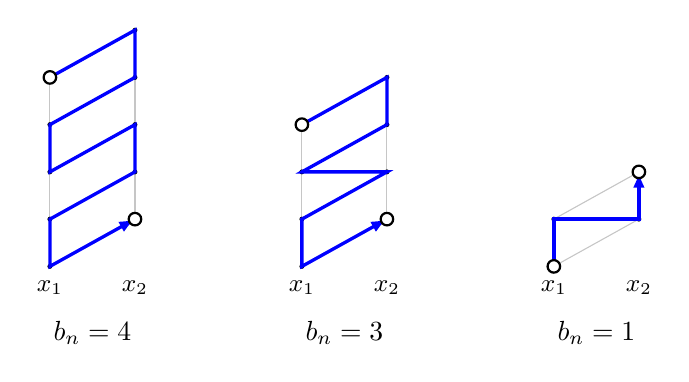
\begin{tikzpicture}
% The gadget: the pillars above consecutive elements x_1 < x_2 of P' (x_2 covers x_1) traversed as one unit.
% (x_1,j) is drawn at height j, (x_2,j) at height j+1, so that heights are ranks.
\def\w{1.8}
\tikzset{ham/.style={Blue,very thick,-{Latex[length=2mm]}},
         unit/.style={draw=black,fill=white,thick,circle,inner sep=1.6pt}}
\newcommand{\pillars}[1]{% faint cover relations of the two pillars of height #1
  \foreach \j in {1,...,#1} {\draw[gray!45] (0,\j-1) -- (0,\j); \draw[gray!45] (\w,\j) -- (\w,\j+1);}
  \foreach \j in {0,...,#1} {\draw[gray!45] (0,\j) -- (\w,\j+1); \fill (0,\j) circle (1.5pt); \fill (\w,\j+1) circle (1.5pt);}
  \node[below] at (0,-0.1) {\small $x_1$}; \node[below] at (\w,-0.1) {\small $x_2$};}

% b_n even, here 4: rows from the top, alternating
\begin{scope}[scale=0.6]
  \pillars{4}
  \draw[ham] plot coordinates {(0,4) (\w,5) (\w,4) (0,3) (0,2) (\w,3) (\w,2) (0,1) (0,0) (\w,1)};
  \node[unit] at (0,4) {}; \node[unit] at (\w,1) {};
  \node at (0.9,-1.4) {$b_n=4$};
\end{scope}

% b_n odd, here 3: one same-rank jump from (x_1,2) to (x_2,1)
\begin{scope}[xshift=3.2cm,scale=0.6]
  \pillars{3}
  \draw[ham] plot coordinates {(0,3) (\w,4) (\w,3) (0,2) (\w,2) (0,1) (0,0) (\w,1)};
  \node[unit] at (0,3) {}; \node[unit] at (\w,1) {};
  \node at (0.9,-1.4) {$b_n=3$};
\end{scope}

% b_n = 1: upwards, with one jump
\begin{scope}[xshift=6.4cm,scale=0.6]
  \pillars{1}
  \draw[ham] plot coordinates {(0,0) (0,1) (\w,1) (\w,2)};
  \node[unit] at (0,0) {}; \node[unit] at (\w,2) {};
  \node at (0.9,-1.4) {$b_n=1$};
\end{scope}
\end{tikzpicture}

	\caption{The gadget for odd $N$: the pillars above consecutive elements $x_1<x_2$ of $P'$, drawn so that heights are ranks, are traversed as a single unit (blue) from one circled vertex to the other. Horizontal steps connect elements of the same rank. Left: $b_n$ even. Middle: $b_n$ odd, with a single same-rank step. Right: $b_n=1$.}
	\label{fig:gadget}
\end{figure}
To prove the theorem, we show that products of chains have mountain range representations:
\begin{proof}[Proof of \Cref{thm:multisetcombinationsfull}]
	Let $P=C_{b_1}\times\ldots\times C_{b_n}$ be a product of chains. We proceed via
	induction. For $n=3$, \Cref{lem:grid-mountain-seed} provides a mountain range representation of $P$, proving the induction start.
	Next, assume that $P'=C_{b_1}\times\ldots\times C_{b_{n-1}}$ admits a mountain range
	representation. We picture the elements of $P'=(x_1,\ldots,x_N)$ to be laid out around a cylinder, with the ranks on circles of
	common height, i.e. with $x_m$ placed at cylindrical coordinates $(2\pi m/N, h,1)$, where $h$ is the rank of
    $x_m$. Stack copies of $P'\times\{x\}$ for $x=0,\ldots,b_n$ on top of each other. The vertical stacks are called \emph{pillars}. If $N$ is
	even, then the new ordering is simply obtained by zigzagging through this picture; in the following argument, pillar indices are read cyclically:
	\[(x_1,0)-\ldots-(x_1,b_n)-(x_2,b_n)-\ldots-(x_2,0)-\ldots\]
	To see that this is a mountain range representation, we first note that properties (i) and (ii)
	are
	trivially fulfilled. To establish property (iii), consider two elements $(x_i,k)$ and $(x_j,k')$
	of the same rank, with no other element of that rank between them. If $k$ and $k'$ are not both
	$0$ or $b_n$, then $x_i$ and $x_j$ are consecutive in the cyclic ordering. If their ranks differ, the cover relation between them together with a vertical cover relation connects $(x_i,k)$ and $(x_j,k')$. If $k=k'$, then the ranks of $x_i$ and $x_j$ must be equal, and hence they
	are related via a pair of cover relations of $P'$. Indeed, all elements of $P'$ on the cyclic arc between $x_i$ and $x_j$ have ranks different from the common rank of $x_i$ and $x_j$, so $x_i$ and $x_j$ are consecutive in the Gray code of their rank in $P'$. Finally, if one of the two elements lies at level $0$ and the other at level $b_n$, then the ranks of $x_i$ and $x_j$ differ by $b_n$, while all elements of $P'$ between them have ranks outside of this range. As the ranks change by at most one along the ordering of $P'$, this is only possible if $b_n=1$ and the two pillars are consecutive in the cyclic ordering, which was covered above. If $N$ is odd, then the zigzagging does not
	close to a cycle. In this case, we traverse the pillars above one pair of consecutive elements as a single unit, see \Cref{fig:gadget}. Since $P'$ has more than one rank, some pair of consecutive elements forms a cover relation. After rotating, and possibly reversing, the ordering of $P'$ we may assume that $x_1<x_2$ is such a pair. If $b_n\ge 2$, we enter the pillar above $x_1$ at the top and traverse the two pillars row by row from the top, alternating between them:
	\[(x_1,b_n)-(x_2,b_n)-(x_2,b_n-1)-(x_1,b_n-1)-(x_1,b_n-2)-\ldots\]
	If $b_n$ is even, this ends in $(x_2,0)$. If $b_n$ is odd, we finish with $(x_1,2)-(x_2,1)-(x_1,1)-(x_1,0)-(x_2,0)$. The step from $(x_1,2)$ to $(x_2,1)$ has equal ranks and differs by a single replacement; the traversal again ends in $(x_2,0)$. If $b_n=1$, we use $(x_1,0)-(x_1,1)-(x_2,0)-(x_2,1)$ instead, which enters at the bottom and leaves at the top. The pillars above $x_3,\ldots,x_N$ are then traversed alternately upwards and downwards as before. As the two pillars above $x_1$ and $x_2$ act as a single pillar, the number of pillars is now even and the ordering closes up. Within the gadget, every rank contains at most one element above $x_1$ and at most one element above $x_2$, and the one above $x_1$ comes first, exactly as in the zigzag. Hence the orderings on the ranks are the same as before, and property (iii) follows as in the case that $N$ is even.
\end{proof}

\begin{figure}
	\centering
	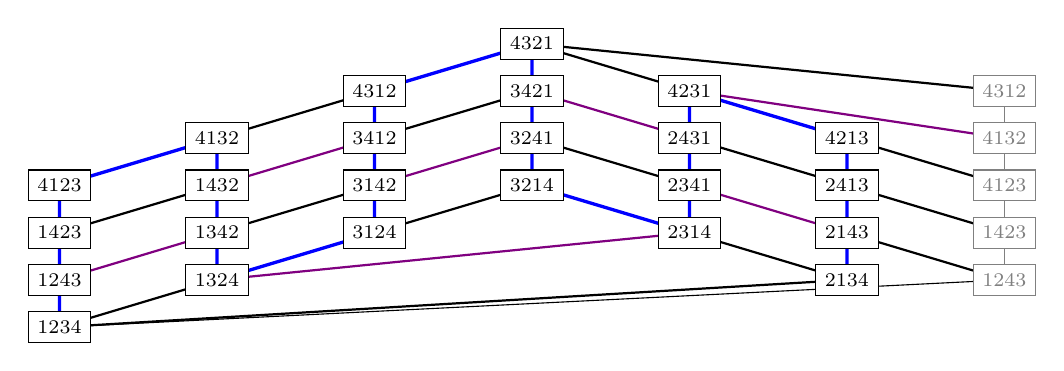
\begin{tikzpicture}[scale=.5, yscale=1.2]
    \coordinate (1234) at (0,0);
    \coordinate (1243) at (0,1);
    \coordinate (1423) at (0,2);
    \coordinate (4123) at (0,3);
    \coordinate (4132) at (4,4);
    \coordinate (1432) at (4,3);
    \coordinate (1342) at (4,2);
    \coordinate (1324) at (4,1);
    \coordinate (3124) at (8,2);
    \coordinate (3142) at (8,3);
    \coordinate (3412) at (8,4);
    \coordinate (4312) at (8,5);
    \coordinate (4321) at (12,6);
    \coordinate (3421) at (12,5);
    \coordinate (3241) at (12,4);
    \coordinate (3214) at (12,3);
    \coordinate (2314) at (16,2);
    \coordinate (2341) at (16,3);
    \coordinate (2431) at (16,4);
    \coordinate (4231) at (16,5);
    \coordinate (4213) at (20,4);
    \coordinate (2413) at (20,3);
    \coordinate (2143) at (20,2);
    \coordinate (2134) at (20,1);
    
    \coordinate (1243e) at (24,1);
    \coordinate (1423e) at (24,2);
    \coordinate (4123e) at (24,3);
    \coordinate (4132e) at (24,4);
    \coordinate (4312e) at (24,5);
    
    \draw[very thick, Blue] (1234) -- (1243) -- (1423) -- (4123) -- (4132) -- (1432) -- (1342) -- (1324) -- (3124) -- (3142) -- (3412) -- (4312) -- (4321) -- (3421) -- (3241) -- (3214) -- (2314) -- (2341) -- (2431) -- (4231) -- (4213) -- (2413) -- (2143) -- (2134);

    \foreach\a/\b in {1234/1324, 1423/1432, 1342/3142, 4132/4312, 3124/3214, 3412/3421, 3241/2341, 4321/4231, 2431/2413, 2314/2134, 1234/2134,4321/4312e,4213/4123e,2413/1423e,2143/1243e}{
        \draw[thick] (\a) -- (\b);
    }
    \foreach\a/\b in {1243/1342, 1432/3412, 1324/2314, 3142/3241, 3421/2431, 2341/2143,4231/4132e}{
        \draw[thick, Purple] (\a) -- (\b);
    }

    \foreach\a/\b in {1243/1423, 1423/4123, 4123/4132, 4132/4312}{
        \draw[gray] (\a e) -- (\b e);
    }
    \draw (1234) -- (1243e);

    \foreach\x in {1234,1243,1423,4123,4132,1432,1342,1324,3124,3142,3412,4312,4321,3421,3241,3214,2314,2341,2431,4231,4213,2413,2143,2134}{
        \node at (\x) [draw, rectangle, fill=white] {\scriptsize$\x$};
    }

    \foreach\x in {1243, 1423, 4123, 4132, 4312}{
        \node at (\x e) [draw=gray, text=gray, rectangle, fill=white] {\scriptsize$\x$};
    }
    
\end{tikzpicture}
	\caption{An (almost) rhombic strip of $\mathcal W_4$. The edges of the product of chains not present in $\mathcal W_4$ are drawn in purple. The SJT Gray code is drawn in blue. Note that the vertices are labeled by their permutations. The zigzagging of the SJT Gray code moves 4 back and forth. When applying the bijection to $C_1\times C_2\times C_3$, the third component is incremented or decremented instead.}
	\label{fig:weakBruhat4}
\end{figure}

\weakBruhat*
\begin{proof}
	The weak Bruhat order $\mathcal{W}_n$ orders permutations of $[n]$ by inclusion of their inversion sets, with cover relations corresponding to adjacent transpositions.

	Consider the product of chains $P = C_1 \times C_2 \times \cdots \times C_{n-1}$. There is a natural bijection between $S_n$ and $P$ mapping a permutation $\pi$ to the tuple $(x_2, \ldots, x_n)$, where $x_i$ is the number of elements smaller than $i$ that appear to the right of $i$ in $\pi$. The diagram of $\mathcal{W}_n$ is a spanning subgraph of the diagram of $P$: incrementing $x_i$ in $P$ swaps $i$ with the first smaller element to its left in $\pi$, which is a cover relation in $\mathcal{W}_n$ if and only if that smaller element is adjacent to $i$.

	We proceed by induction on $n$ with the following claim: The cyclic rhombic strip $R$ of $P$ obtained via the zigzagging construction contains the SJT Gray code as its $c$-monotone Hamilton cycle, and deleting the edges of $P \setminus \mathcal{W}_n$ from $R$ yields an embedding where every face has degree 4 or 6.

	The base case $n=4$ is illustrated in \Cref{fig:weakBruhat4}. For the inductive step, applying the zigzagging construction adds the chain $C_{n-1}$. By definition, this routes the path back and forth across the layers, effectively sweeping the position of the element $n$ through the permutation. This precisely matches the recursive definition of the SJT Gray code.

	In this construction, new rhombi are formed between the vertical chains connecting copies of the Hamilton cycle. Ignoring $n$, any two adjacent vertical chains differ by an adjacent transposition. As $n$ sweeps through the permutation, it acts as an obstruction exactly once per adjacent pair of $C_{n-1}$. Consequently, exactly one edge is missing between these adjacent chains, see \Cref{fig:weakBruhat4}.

	The resulting structure is an (almost) cyclic rhombic strip for $\mathcal{W}_n$ where all faces have degree 4 or 6. Because the maximum face degree is 6, adjacent elements along any common rank (permutations with exactly $k$ inversions) remain connected by a path of length two. Thus, they are related by a pair of cover relations.
\end{proof}

\subsection{Cartesian Products}

\begin{figure}[!ht]
	\centering
	
\def\lensangle{40}
\def\xstep{2.5cm}
\def\ystep{1.5cm}
\def\scew{5}
\def\height{3}

\newcommand{\lens}[2]{
\begin{scope}[xshift=#1*\xstep, yshift=#2*\ystep]
    
    \filldraw[draw=black,fill=white] 
        (\scew,\height) to[bend left=\lensangle] (-\scew,-\height) 
        to[bend left=\lensangle] (\scew,\height) -- cycle;
    % Move the node inside the path construction
\path (\scew,\height) to[bend left=\lensangle] node[pos=0.5, above] {$R_-$} (-\scew,-\height);
\path (-\scew,-\height) to[bend left=\lensangle] node[pos=0.5, below] {$R^-$} (\scew,\height);

    \node[circle, fill, inner sep=2pt] (lenstop#1#2) at (\scew,\height) {};
    \node[circle, fill, inner sep=2pt] (lensbottom#1#2) at (-\scew,-\height) {};
        
\end{scope}
}

    \begin{tikzpicture}[scale=0.5]

        \lens{0}{0}

        \draw[thick,Orange] 
        (lensbottom00) -- 
        ++(3,3) -- 
        ++(1,-1) -- 
        ++(3,3) --
        ++(1,-1) --
        ++(2,2);

        \draw[-{Latex[length=2.5mm, width=1.5mm]}] (5,0) -- (6,0);

        \node[circle, fill, inner sep=2pt] (bb) at (7,-2-\height) {};
        \node[circle, fill, inner sep=2pt] (bt) at (17,-2+\height) {};
        \node[circle, fill, inner sep=2pt] (tb) at (7,+2-\height) {};
        \node[circle, fill, inner sep=2pt] (tt) at (17,+2+\height) {};

        \draw (bb) to[bend right=\lensangle] (bt);
        \draw (tb) to[bend left=\lensangle] (tt);
        \draw (bb) -- (tb) (bt) -- (tt);

        \path (bb) to[bend right=\lensangle] node[pos=0.5, above] {$R_-$} (bt);
        \path (tb) to[bend left=\lensangle] node[pos=0.5, below] {$R^-$} (tt);

        \draw[thick,Orange] 
        (bb) -- 
        ++(3,3) -- 
        ++(1,-1) -- 
        ++(3,3) --
        ++(1,-1) --
        ++(2,2);
        
        \draw[thick,Orange] 
        (tb) -- 
        ++(3,3) -- 
        ++(1,-1) -- 
        ++(3,3) --
        ++(1,-1) --
        ++(2,2);



        \draw
        (bb) ++(0,1) -- 
        ++(3,3) -- 
        ++(1,-1) -- 
        ++(3,3) --
        ++(1,-1) --
        ++(2,2);
        \draw
        (bb) ++(0,2) -- 
        ++(3,3) -- 
        ++(1,-1) -- 
        ++(3,3) --
        ++(1,-1) --
        ++(2,2);
        \draw
        (bb) ++(0,3) -- 
        ++(3,3) -- 
        ++(1,-1) -- 
        ++(3,3) --
        ++(1,-1) --
        ++(2,2);

        \def\lensangle{20}
        \def\xstep{1cm}
        \def\ystep{1cm}
        \def\scew{0}
        \def\height{2}
        \renewcommand{\lens}[2]{
\begin{scope}[xshift=#1*\xstep, yshift=#2*\ystep]
    
    \filldraw[draw=black,fill=white] 
        (\scew,\height) to[bend left=\lensangle] (-\scew,-\height) 
        to[bend left=\lensangle] (\scew,\height) -- cycle;

    \node (lenstop#1#2) at (\scew,\height) {};
    \node (lensbottom#1#2) at (-\scew,-\height) {};
        
    \pgfmathtruncatemacro\sign{mod(#1,2)}
    \if\sign 0{\draw[-{Latex[length=2.5mm, width=1.5mm]}] (-0.3,0) -- (0.3,0);}\else{\draw[{Latex[length=2.5mm, width=1.5mm]}-] (-0.3,0) -- (0.3,0);}\fi
\end{scope}}
\begin{scope}[xshift=7cm,yshift=-3cm]

        
        \foreach\x/\y in {0/0,1/1,2/2,3/3,4/2,5/3,6/4,7/5,8/4,9/5,10/6}
        {\lens{\x}{\y}}
\end{scope}

\foreach\x in {bb,bt,tb,tt}{
    \node[circle, fill, inner sep=2pt] at (\x) {};
}
        
    \end{tikzpicture}
	\caption{Combining zigzagging with unfolding yields the product construction.}
	\label{fig:product}
\end{figure}

\products*
\begin{proof}
	The construction for the product $P \times Q$ combines unfolding and zigzagging, see \Cref{fig:product}. Let $R_P$ be a (cyclic) Hamiltonian rhombic strip of $P$ with a $c$-monotone Hamilton path (or cycle) $H = (x_1, \ldots, x_m)$, and let $R_Q$ be a non-cyclic rhombic strip of $Q$.

	As in the zigzagging construction, we split $R_P$ along $H$, separating it into a lower sub-drawing $R_{P-}$ and an upper sub-drawing $R_P^-$. Rather than bridging the gap with chains, we embed a sequence of copies of $R_Q$ as in the unfolding construction: For each $i \in \{1, \ldots, m\}$, we insert a copy $R_{Q,i}$ of $R_Q$. To enable crossing-free connections between adjacent copies, we apply a horizontal reflection to $R_{Q,i}$ for every alternating index $i$.

	We then anchor these copies to the split strip $R_P$: the minimum of each $R_{Q,i}$ is identified with the vertex $x_i$ in the lower layer $R_{P-}$, and its global maximum is identified with the copy of $x_i$ in the upper layer $R_P^-$.

	Next, we add the edges corresponding to the covering relations between adjacent copies of $Q$. Following the unfolding construction, the alternating reflections ensure that the corresponding left and right boundary chains of $R_{Q,i}$ and $R_{Q,i+1}$ face one another. Thus, we can insert the edges connecting these matched boundaries without introducing any crossings. This completes the (cyclic) rhombic strip for $P \times Q$. As in the proof of \Cref{thm:zigzagging}, note that $P$ must have an even number of vertices if it admits a cyclic Hamiltonian rhombic strip.

	Finally, if $R_Q$ is also Hamiltonian, each copy $R_{Q,i}$ contains its own Hamilton path. These can be concatenated into a Hamilton path (or cycle).
\end{proof}

\subsection{Tree Associahedra}

\begin{figure}[!ht]
	\centering
	
\newsavebox{\boxshapea}
\sbox{\boxshapea}{
  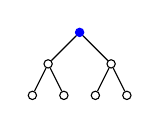
\begin{tikzpicture}[baseline=-0.5ex, scale=0.4]
    \tikzset{every node/.style={draw, circle, inner sep=0.5pt, minimum size=3pt}}
    \node[] (N4) at (-1.50, -2) {};
    \node[] (N5) at (-0.50, -2) {};
    \node[] (N2) at (-1.00, -1) {};
    \node[] (N6) at (0.50, -2) {};
    \node[] (N7) at (1.50, -2) {};
    \node[] (N3) at (1.00, -1) {};
    \node[fill=Blue, draw=Blue] (N1) at (0.00, 0) {};
    \draw (N1) -- (N2);
    \draw (N2) -- (N4);
    \draw (N2) -- (N5);
    \draw (N1) -- (N3);
    \draw (N3) -- (N6);
    \draw (N3) -- (N7);
  \end{tikzpicture}
}
\newsavebox{\boxshapeb}
\sbox{\boxshapeb}{
  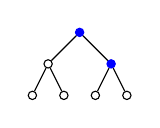
\begin{tikzpicture}[baseline=-0.5ex, scale=0.4]
    \tikzset{every node/.style={draw, circle, inner sep=0.5pt, minimum size=3pt}}
    \node[] (N4) at (-1.50, -2) {};
    \node[] (N5) at (-0.50, -2) {};
    \node[] (N2) at (-1.00, -1) {};
    \node[] (N6) at (0.50, -2) {};
    \node[] (N7) at (1.50, -2) {};
    \node[fill=Blue, draw=Blue] (N3) at (1.00, -1) {};
    \node[fill=Blue, draw=Blue] (N1) at (0.00, 0) {};
    \draw (N1) -- (N2);
    \draw (N2) -- (N4);
    \draw (N2) -- (N5);
    \draw (N1) -- (N3);
    \draw (N3) -- (N6);
    \draw (N3) -- (N7);
  \end{tikzpicture}
}
\newsavebox{\boxshapec}
\sbox{\boxshapec}{
  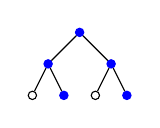
\begin{tikzpicture}[baseline=-0.5ex, scale=0.4]
    \tikzset{every node/.style={draw, circle, inner sep=0.5pt, minimum size=3pt}}
    \node[] (N4) at (-1.50, -2) {};
    \node[fill=Blue, draw=Blue] (N5) at (-0.50, -2) {};
    \node[fill=Blue, draw=Blue] (N2) at (-1.00, -1) {};
    \node[] (N6) at (0.50, -2) {};
    \node[fill=Blue, draw=Blue] (N7) at (1.50, -2) {};
    \node[fill=Blue, draw=Blue] (N3) at (1.00, -1) {};
    \node[fill=Blue, draw=Blue] (N1) at (0.00, 0) {};
    \draw (N1) -- (N2);
    \draw (N2) -- (N4);
    \draw (N2) -- (N5);
    \draw (N1) -- (N3);
    \draw (N3) -- (N6);
    \draw (N3) -- (N7);
  \end{tikzpicture}
}
\newsavebox{\boxshaped}
\sbox{\boxshaped}{
  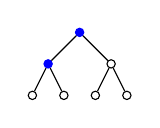
\begin{tikzpicture}[baseline=-0.5ex, scale=0.4]
    \tikzset{every node/.style={draw, circle, inner sep=0.5pt, minimum size=3pt}}
    \node[] (N4) at (-1.50, -2) {};
    \node[] (N5) at (-0.50, -2) {};
    \node[fill=Blue, draw=Blue] (N2) at (-1.00, -1) {};
    \node[] (N6) at (0.50, -2) {};
    \node[] (N7) at (1.50, -2) {};
    \node[] (N3) at (1.00, -1) {};
    \node[fill=Blue, draw=Blue] (N1) at (0.00, 0) {};
    \draw (N1) -- (N2);
    \draw (N2) -- (N4);
    \draw (N2) -- (N5);
    \draw (N1) -- (N3);
    \draw (N3) -- (N6);
    \draw (N3) -- (N7);
  \end{tikzpicture}
}
\newsavebox{\boxshapee}
\sbox{\boxshapee}{
  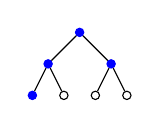
\begin{tikzpicture}[baseline=-0.5ex, scale=0.4]
    \tikzset{every node/.style={draw, circle, inner sep=0.5pt, minimum size=3pt}}
    \node[fill=Blue, draw=Blue] (N4) at (-1.50, -2) {};
    \node[] (N5) at (-0.50, -2) {};
    \node[fill=Blue, draw=Blue] (N2) at (-1.00, -1) {};
    \node[] (N6) at (0.50, -2) {};
    \node[] (N7) at (1.50, -2) {};
    \node[fill=Blue, draw=Blue] (N3) at (1.00, -1) {};
    \node[fill=Blue, draw=Blue] (N1) at (0.00, 0) {};
    \draw (N1) -- (N2);
    \draw (N2) -- (N4);
    \draw (N2) -- (N5);
    \draw (N1) -- (N3);
    \draw (N3) -- (N6);
    \draw (N3) -- (N7);
  \end{tikzpicture}
}
\newsavebox{\boxshapef}
\sbox{\boxshapef}{
  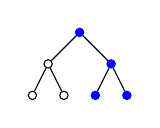
\begin{tikzpicture}[baseline=-0.5ex, scale=0.4]
    \tikzset{every node/.style={draw, circle, inner sep=0.5pt, minimum size=3pt}}
    \node[] (N4) at (-1.50, -2) {};
    \node[] (N5) at (-0.50, -2) {};
    \node[] (N2) at (-1.00, -1) {};
    \node[fill=Blue, draw=Blue] (N6) at (0.50, -2) {};
    \node[fill=Blue, draw=Blue] (N7) at (1.50, -2) {};
    \node[fill=Blue, draw=Blue] (N3) at (1.00, -1) {};
    \node[fill=Blue, draw=Blue] (N1) at (0.00, 0) {};
    \draw (N1) -- (N2);
    \draw (N2) -- (N4);
    \draw (N2) -- (N5);
    \draw (N1) -- (N3);
    \draw (N3) -- (N6);
    \draw (N3) -- (N7);
  \end{tikzpicture}
}
\newsavebox{\boxshapeg}
\sbox{\boxshapeg}{
  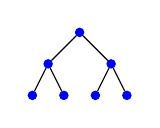
\begin{tikzpicture}[baseline=-0.5ex, scale=0.4]
    \tikzset{every node/.style={draw, circle, inner sep=0.5pt, minimum size=3pt}}
    \node[fill=Blue, draw=Blue] (N4) at (-1.50, -2) {};
    \node[fill=Blue, draw=Blue] (N5) at (-0.50, -2) {};
    \node[fill=Blue, draw=Blue] (N2) at (-1.00, -1) {};
    \node[fill=Blue, draw=Blue] (N6) at (0.50, -2) {};
    \node[fill=Blue, draw=Blue] (N7) at (1.50, -2) {};
    \node[fill=Blue, draw=Blue] (N3) at (1.00, -1) {};
    \node[fill=Blue, draw=Blue] (N1) at (0.00, 0) {};
    \draw (N1) -- (N2);
    \draw (N2) -- (N4);
    \draw (N2) -- (N5);
    \draw (N1) -- (N3);
    \draw (N3) -- (N6);
    \draw (N3) -- (N7);
  \end{tikzpicture}
}
\newsavebox{\boxshapeh}
\sbox{\boxshapeh}{
  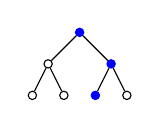
\begin{tikzpicture}[baseline=-0.5ex, scale=0.4]
    \tikzset{every node/.style={draw, circle, inner sep=0.5pt, minimum size=3pt}}
    \node[] (N4) at (-1.50, -2) {};
    \node[] (N5) at (-0.50, -2) {};
    \node[] (N2) at (-1.00, -1) {};
    \node[fill=Blue, draw=Blue] (N6) at (0.50, -2) {};
    \node[] (N7) at (1.50, -2) {};
    \node[fill=Blue, draw=Blue] (N3) at (1.00, -1) {};
    \node[fill=Blue, draw=Blue] (N1) at (0.00, 0) {};
    \draw (N1) -- (N2);
    \draw (N2) -- (N4);
    \draw (N2) -- (N5);
    \draw (N1) -- (N3);
    \draw (N3) -- (N6);
    \draw (N3) -- (N7);
  \end{tikzpicture}
}
\newsavebox{\boxshapei}
\sbox{\boxshapei}{
  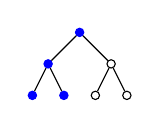
\begin{tikzpicture}[baseline=-0.5ex, scale=0.4]
    \tikzset{every node/.style={draw, circle, inner sep=0.5pt, minimum size=3pt}}
    \node[fill=Blue, draw=Blue] (N4) at (-1.50, -2) {};
    \node[fill=Blue, draw=Blue] (N5) at (-0.50, -2) {};
    \node[fill=Blue, draw=Blue] (N2) at (-1.00, -1) {};
    \node[] (N6) at (0.50, -2) {};
    \node[] (N7) at (1.50, -2) {};
    \node[] (N3) at (1.00, -1) {};
    \node[fill=Blue, draw=Blue] (N1) at (0.00, 0) {};
    \draw (N1) -- (N2);
    \draw (N2) -- (N4);
    \draw (N2) -- (N5);
    \draw (N1) -- (N3);
    \draw (N3) -- (N6);
    \draw (N3) -- (N7);
  \end{tikzpicture}
}
\newsavebox{\boxshapej}
\sbox{\boxshapej}{
  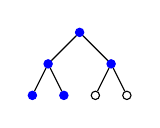
\begin{tikzpicture}[baseline=-0.5ex, scale=0.4]
    \tikzset{every node/.style={draw, circle, inner sep=0.5pt, minimum size=3pt}}
    \node[fill=Blue, draw=Blue] (N4) at (-1.50, -2) {};
    \node[fill=Blue, draw=Blue] (N5) at (-0.50, -2) {};
    \node[fill=Blue, draw=Blue] (N2) at (-1.00, -1) {};
    \node[] (N6) at (0.50, -2) {};
    \node[] (N7) at (1.50, -2) {};
    \node[fill=Blue, draw=Blue] (N3) at (1.00, -1) {};
    \node[fill=Blue, draw=Blue] (N1) at (0.00, 0) {};
    \draw (N1) -- (N2);
    \draw (N2) -- (N4);
    \draw (N2) -- (N5);
    \draw (N1) -- (N3);
    \draw (N3) -- (N6);
    \draw (N3) -- (N7);
  \end{tikzpicture}
}
\newsavebox{\boxshapek}
\sbox{\boxshapek}{
  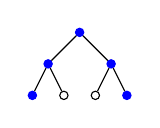
\begin{tikzpicture}[baseline=-0.5ex, scale=0.4]
    \tikzset{every node/.style={draw, circle, inner sep=0.5pt, minimum size=3pt}}
    \node[fill=Blue, draw=Blue] (N4) at (-1.50, -2) {};
    \node[] (N5) at (-0.50, -2) {};
    \node[fill=Blue, draw=Blue] (N2) at (-1.00, -1) {};
    \node[] (N6) at (0.50, -2) {};
    \node[fill=Blue, draw=Blue] (N7) at (1.50, -2) {};
    \node[fill=Blue, draw=Blue] (N3) at (1.00, -1) {};
    \node[fill=Blue, draw=Blue] (N1) at (0.00, 0) {};
    \draw (N1) -- (N2);
    \draw (N2) -- (N4);
    \draw (N2) -- (N5);
    \draw (N1) -- (N3);
    \draw (N3) -- (N6);
    \draw (N3) -- (N7);
  \end{tikzpicture}
}
\newsavebox{\boxshapel}
\sbox{\boxshapel}{
  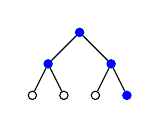
\begin{tikzpicture}[baseline=-0.5ex, scale=0.4]
    \tikzset{every node/.style={draw, circle, inner sep=0.5pt, minimum size=3pt}}
    \node[] (N4) at (-1.50, -2) {};
    \node[] (N5) at (-0.50, -2) {};
    \node[fill=Blue, draw=Blue] (N2) at (-1.00, -1) {};
    \node[] (N6) at (0.50, -2) {};
    \node[fill=Blue, draw=Blue] (N7) at (1.50, -2) {};
    \node[fill=Blue, draw=Blue] (N3) at (1.00, -1) {};
    \node[fill=Blue, draw=Blue] (N1) at (0.00, 0) {};
    \draw (N1) -- (N2);
    \draw (N2) -- (N4);
    \draw (N2) -- (N5);
    \draw (N1) -- (N3);
    \draw (N3) -- (N6);
    \draw (N3) -- (N7);
  \end{tikzpicture}
}
\newsavebox{\boxshapem}
\sbox{\boxshapem}{
  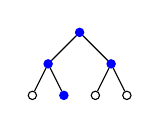
\begin{tikzpicture}[baseline=-0.5ex, scale=0.4]
    \tikzset{every node/.style={draw, circle, inner sep=0.5pt, minimum size=3pt}}
    \node[] (N4) at (-1.50, -2) {};
    \node[fill=Blue, draw=Blue] (N5) at (-0.50, -2) {};
    \node[fill=Blue, draw=Blue] (N2) at (-1.00, -1) {};
    \node[] (N6) at (0.50, -2) {};
    \node[] (N7) at (1.50, -2) {};
    \node[fill=Blue, draw=Blue] (N3) at (1.00, -1) {};
    \node[fill=Blue, draw=Blue] (N1) at (0.00, 0) {};
    \draw (N1) -- (N2);
    \draw (N2) -- (N4);
    \draw (N2) -- (N5);
    \draw (N1) -- (N3);
    \draw (N3) -- (N6);
    \draw (N3) -- (N7);
  \end{tikzpicture}
}
\newsavebox{\boxshapen}
\sbox{\boxshapen}{
  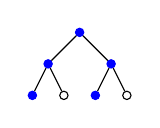
\begin{tikzpicture}[baseline=-0.5ex, scale=0.4]
    \tikzset{every node/.style={draw, circle, inner sep=0.5pt, minimum size=3pt}}
    \node[fill=Blue, draw=Blue] (N4) at (-1.50, -2) {};
    \node[] (N5) at (-0.50, -2) {};
    \node[fill=Blue, draw=Blue] (N2) at (-1.00, -1) {};
    \node[fill=Blue, draw=Blue] (N6) at (0.50, -2) {};
    \node[] (N7) at (1.50, -2) {};
    \node[fill=Blue, draw=Blue] (N3) at (1.00, -1) {};
    \node[fill=Blue, draw=Blue] (N1) at (0.00, 0) {};
    \draw (N1) -- (N2);
    \draw (N2) -- (N4);
    \draw (N2) -- (N5);
    \draw (N1) -- (N3);
    \draw (N3) -- (N6);
    \draw (N3) -- (N7);
  \end{tikzpicture}
}
\newsavebox{\boxshapeo}
\sbox{\boxshapeo}{
  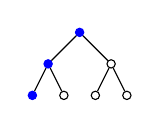
\begin{tikzpicture}[baseline=-0.5ex, scale=0.4]
    \tikzset{every node/.style={draw, circle, inner sep=0.5pt, minimum size=3pt}}
    \node[fill=Blue, draw=Blue] (N4) at (-1.50, -2) {};
    \node[] (N5) at (-0.50, -2) {};
    \node[fill=Blue, draw=Blue] (N2) at (-1.00, -1) {};
    \node[] (N6) at (0.50, -2) {};
    \node[] (N7) at (1.50, -2) {};
    \node[] (N3) at (1.00, -1) {};
    \node[fill=Blue, draw=Blue] (N1) at (0.00, 0) {};
    \draw (N1) -- (N2);
    \draw (N2) -- (N4);
    \draw (N2) -- (N5);
    \draw (N1) -- (N3);
    \draw (N3) -- (N6);
    \draw (N3) -- (N7);
  \end{tikzpicture}
}
\newsavebox{\boxshapep}
\sbox{\boxshapep}{
  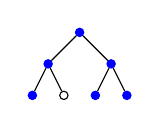
\begin{tikzpicture}[baseline=-0.5ex, scale=0.4]
    \tikzset{every node/.style={draw, circle, inner sep=0.5pt, minimum size=3pt}}
    \node[fill=Blue, draw=Blue] (N4) at (-1.50, -2) {};
    \node[] (N5) at (-0.50, -2) {};
    \node[fill=Blue, draw=Blue] (N2) at (-1.00, -1) {};
    \node[fill=Blue, draw=Blue] (N6) at (0.50, -2) {};
    \node[fill=Blue, draw=Blue] (N7) at (1.50, -2) {};
    \node[fill=Blue, draw=Blue] (N3) at (1.00, -1) {};
    \node[fill=Blue, draw=Blue] (N1) at (0.00, 0) {};
    \draw (N1) -- (N2);
    \draw (N2) -- (N4);
    \draw (N2) -- (N5);
    \draw (N1) -- (N3);
    \draw (N3) -- (N6);
    \draw (N3) -- (N7);
  \end{tikzpicture}
}
\newsavebox{\boxshapeq}
\sbox{\boxshapeq}{
  \begin{tikzpicture}[baseline=-0.5ex, scale=0.4]
    \tikzset{every node/.style={draw, circle, inner sep=0.5pt, minimum size=3pt}}
    \node[] (N4) at (-1.50, -2) {};
    \node[] (N5) at (-0.50, -2) {};
    \node[fill=Blue, draw=Blue] (N2) at (-1.00, -1) {};
    \node[fill=Blue, draw=Blue] (N6) at (0.50, -2) {};
    \node[] (N7) at (1.50, -2) {};
    \node[fill=Blue, draw=Blue] (N3) at (1.00, -1) {};
    \node[fill=Blue, draw=Blue] (N1) at (0.00, 0) {};
    \draw (N1) -- (N2);
    \draw (N2) -- (N4);
    \draw (N2) -- (N5);
    \draw (N1) -- (N3);
    \draw (N3) -- (N6);
    \draw (N3) -- (N7);
  \end{tikzpicture}
}
\newsavebox{\boxshaper}
\sbox{\boxshaper}{
  \begin{tikzpicture}[baseline=-0.5ex, scale=0.4]
    \tikzset{every node/.style={draw, circle, inner sep=0.5pt, minimum size=3pt}}
    \node[] (N4) at (-1.50, -2) {};
    \node[fill=Blue, draw=Blue] (N5) at (-0.50, -2) {};
    \node[fill=Blue, draw=Blue] (N2) at (-1.00, -1) {};
    \node[] (N6) at (0.50, -2) {};
    \node[] (N7) at (1.50, -2) {};
    \node[] (N3) at (1.00, -1) {};
    \node[fill=Blue, draw=Blue] (N1) at (0.00, 0) {};
    \draw (N1) -- (N2);
    \draw (N2) -- (N4);
    \draw (N2) -- (N5);
    \draw (N1) -- (N3);
    \draw (N3) -- (N6);
    \draw (N3) -- (N7);
  \end{tikzpicture}
}
\newsavebox{\boxshapes}
\sbox{\boxshapes}{
  \begin{tikzpicture}[baseline=-0.5ex, scale=0.4]
    \tikzset{every node/.style={draw, circle, inner sep=0.5pt, minimum size=3pt}}
    \node[] (N4) at (-1.50, -2) {};
    \node[fill=Blue, draw=Blue] (N5) at (-0.50, -2) {};
    \node[fill=Blue, draw=Blue] (N2) at (-1.00, -1) {};
    \node[fill=Blue, draw=Blue] (N6) at (0.50, -2) {};
    \node[] (N7) at (1.50, -2) {};
    \node[fill=Blue, draw=Blue] (N3) at (1.00, -1) {};
    \node[fill=Blue, draw=Blue] (N1) at (0.00, 0) {};
    \draw (N1) -- (N2);
    \draw (N2) -- (N4);
    \draw (N2) -- (N5);
    \draw (N1) -- (N3);
    \draw (N3) -- (N6);
    \draw (N3) -- (N7);
  \end{tikzpicture}
}
\newsavebox{\boxshapet}
\sbox{\boxshapet}{
  \begin{tikzpicture}[baseline=-0.5ex, scale=0.4]
    \tikzset{every node/.style={draw, circle, inner sep=0.5pt, minimum size=3pt}}
    \node[] (N4) at (-1.50, -2) {};
    \node[] (N5) at (-0.50, -2) {};
    \node[] (N2) at (-1.00, -1) {};
    \node[] (N6) at (0.50, -2) {};
    \node[fill=Blue, draw=Blue] (N7) at (1.50, -2) {};
    \node[fill=Blue, draw=Blue] (N3) at (1.00, -1) {};
    \node[fill=Blue, draw=Blue] (N1) at (0.00, 0) {};
    \draw (N1) -- (N2);
    \draw (N2) -- (N4);
    \draw (N2) -- (N5);
    \draw (N1) -- (N3);
    \draw (N3) -- (N6);
    \draw (N3) -- (N7);
  \end{tikzpicture}
}
\newsavebox{\boxshapeu}
\sbox{\boxshapeu}{
  \begin{tikzpicture}[baseline=-0.5ex, scale=0.4]
    \tikzset{every node/.style={draw, circle, inner sep=0.5pt, minimum size=3pt}}
    \node[] (N4) at (-1.50, -2) {};
    \node[] (N5) at (-0.50, -2) {};
    \node[fill=Blue, draw=Blue] (N2) at (-1.00, -1) {};
    \node[fill=Blue, draw=Blue] (N6) at (0.50, -2) {};
    \node[fill=Blue, draw=Blue] (N7) at (1.50, -2) {};
    \node[fill=Blue, draw=Blue] (N3) at (1.00, -1) {};
    \node[fill=Blue, draw=Blue] (N1) at (0.00, 0) {};
    \draw (N1) -- (N2);
    \draw (N2) -- (N4);
    \draw (N2) -- (N5);
    \draw (N1) -- (N3);
    \draw (N3) -- (N6);
    \draw (N3) -- (N7);
  \end{tikzpicture}
}
\newsavebox{\boxshapev}
\sbox{\boxshapev}{
  \begin{tikzpicture}[baseline=-0.5ex, scale=0.4]
    \tikzset{every node/.style={draw, circle, inner sep=0.5pt, minimum size=3pt}}
    \node[] (N4) at (-1.50, -2) {};
    \node[] (N5) at (-0.50, -2) {};
    \node[fill=Blue, draw=Blue] (N2) at (-1.00, -1) {};
    \node[] (N6) at (0.50, -2) {};
    \node[] (N7) at (1.50, -2) {};
    \node[fill=Blue, draw=Blue] (N3) at (1.00, -1) {};
    \node[fill=Blue, draw=Blue] (N1) at (0.00, 0) {};
    \draw (N1) -- (N2);
    \draw (N2) -- (N4);
    \draw (N2) -- (N5);
    \draw (N1) -- (N3);
    \draw (N3) -- (N6);
    \draw (N3) -- (N7);
  \end{tikzpicture}
}
\newsavebox{\boxshapew}
\sbox{\boxshapew}{
  \begin{tikzpicture}[baseline=-0.5ex, scale=0.4]
    \tikzset{every node/.style={draw, circle, inner sep=0.5pt, minimum size=3pt}}
    \node[fill=Blue, draw=Blue] (N4) at (-1.50, -2) {};
    \node[fill=Blue, draw=Blue] (N5) at (-0.50, -2) {};
    \node[fill=Blue, draw=Blue] (N2) at (-1.00, -1) {};
    \node[] (N6) at (0.50, -2) {};
    \node[fill=Blue, draw=Blue] (N7) at (1.50, -2) {};
    \node[fill=Blue, draw=Blue] (N3) at (1.00, -1) {};
    \node[fill=Blue, draw=Blue] (N1) at (0.00, 0) {};
    \draw (N1) -- (N2);
    \draw (N2) -- (N4);
    \draw (N2) -- (N5);
    \draw (N1) -- (N3);
    \draw (N3) -- (N6);
    \draw (N3) -- (N7);
  \end{tikzpicture}
}
\newsavebox{\boxshapex}
\sbox{\boxshapex}{
  \begin{tikzpicture}[baseline=-0.5ex, scale=0.4]
    \tikzset{every node/.style={draw, circle, inner sep=0.5pt, minimum size=3pt}}
    \node[] (N4) at (-1.50, -2) {};
    \node[] (N5) at (-0.50, -2) {};
    \node[] (N2) at (-1.00, -1) {};
    \node[] (N6) at (0.50, -2) {};
    \node[] (N7) at (1.50, -2) {};
    \node[] (N3) at (1.00, -1) {};
    \node[] (N1) at (0.00, 0) {};
    \draw (N1) -- (N2);
    \draw (N2) -- (N4);
    \draw (N2) -- (N5);
    \draw (N1) -- (N3);
    \draw (N3) -- (N6);
    \draw (N3) -- (N7);
  \end{tikzpicture}
}
\newsavebox{\boxshapey}
\sbox{\boxshapey}{
  \begin{tikzpicture}[baseline=-0.5ex, scale=0.4]
    \tikzset{every node/.style={draw, circle, inner sep=0.5pt, minimum size=3pt}}
    \node[] (N4) at (-1.50, -2) {};
    \node[fill=Blue, draw=Blue] (N5) at (-0.50, -2) {};
    \node[fill=Blue, draw=Blue] (N2) at (-1.00, -1) {};
    \node[fill=Blue, draw=Blue] (N6) at (0.50, -2) {};
    \node[fill=Blue, draw=Blue] (N7) at (1.50, -2) {};
    \node[fill=Blue, draw=Blue] (N3) at (1.00, -1) {};
    \node[fill=Blue, draw=Blue] (N1) at (0.00, 0) {};
    \draw (N1) -- (N2);
    \draw (N2) -- (N4);
    \draw (N2) -- (N5);
    \draw (N1) -- (N3);
    \draw (N3) -- (N6);
    \draw (N3) -- (N7);
  \end{tikzpicture}
}
\newsavebox{\boxshapez}
\sbox{\boxshapez}{
  \begin{tikzpicture}[baseline=-0.5ex, scale=0.4]
    \tikzset{every node/.style={draw, circle, inner sep=0.5pt, minimum size=3pt}}
    \node[fill=Blue, draw=Blue] (N4) at (-1.50, -2) {};
    \node[fill=Blue, draw=Blue] (N5) at (-0.50, -2) {};
    \node[fill=Blue, draw=Blue] (N2) at (-1.00, -1) {};
    \node[fill=Blue, draw=Blue] (N6) at (0.50, -2) {};
    \node[] (N7) at (1.50, -2) {};
    \node[fill=Blue, draw=Blue] (N3) at (1.00, -1) {};
    \node[fill=Blue, draw=Blue] (N1) at (0.00, 0) {};
    \draw (N1) -- (N2);
    \draw (N2) -- (N4);
    \draw (N2) -- (N5);
    \draw (N1) -- (N3);
    \draw (N3) -- (N6);
    \draw (N3) -- (N7);
  \end{tikzpicture}
}
\begin{tikzpicture}[yscale=1.8,xscale=2.8]
\newcommand{\edgespathclr}{Blue}
\newcommand{\edgesclr}{gray}
\coordinate (1) at (2.00, 1);
\coordinate (1-3) at (0.00, 2);
\coordinate (1-2-3-5-7) at (0.80, 5);
\coordinate (1-2) at (4.00, 2);
\coordinate (1-2-3-4) at (4.00, 4);
\coordinate (1-3-6-7) at (0.00, 4);
\coordinate (1-2-3-4-5-6-7) at (2.00, 7);
\coordinate (1-3-6) at (1.00, 3);
\coordinate (1-2-4-5) at (3.20, 4);
\coordinate (1-2-3-4-5) at (2.40, 5);
\coordinate (1-2-3-4-7) at (3.20, 5);
\coordinate (1-2-3-7) at (1.60, 4);
\coordinate (1-2-3-5) at (2.40, 4);
\coordinate (1-2-3-4-6) at (4.00, 5);
\coordinate (1-2-4) at (4.00, 3);
\coordinate (1-2-3-4-6-7) at (4.00, 6);
\coordinate (1-2-3-6) at (0.80, 4);
\coordinate (1-2-5) at (3.00, 3);
\coordinate (1-2-3-5-6) at (1.60, 5);
\coordinate (1-3-7) at (0.00, 3);
\coordinate (1-2-3-6-7) at (0.00, 5);
\coordinate (1-2-3) at (2.00, 3);
\coordinate (1-2-3-4-5-7) at (2.67, 6);
\coordinate (empty) at (2.00, 0);
\coordinate (1-2-3-5-6-7) at (0.00, 6);
\coordinate (1-2-3-4-5-6) at (1.33, 6);
\foreach\a/\b in {
1-2-3-4/1-2-3-4-6, 1-2-3-4-7/1-2-3-4-5-7, 1-2-3-4-5-7/1-2-3-4-5-6-7, 1-2-3-4-5/1-2-3-4-5-6, 1-2-3-5/1-2-3-4-5, 1-3/1-3-6, 1-3-6-7/1-2-3-6-7, 1/1-2, 1-2-3/1-2-3-7, 1-2-3/1-2-3-5, 1-2-4/1-2-4-5, 1-2-3-7/1-2-3-6-7, 1-2-3-5/1-2-3-5-6, 1-2-3-5-6-7/1-2-3-4-5-6-7, 1-2-3/1-2-3-6, 1-2-3-4/1-2-3-4-5, 1-2/1-2-3, 1-3-6/1-3-6-7, 1-2-3-6-7/1-2-3-5-6-7, 1-2-3-7/1-2-3-5-7, 1-2-3-4-5/1-2-3-4-5-7, 1-2-3-5-6/1-2-3-5-6-7, 1-2-4-5/1-2-3-4-5, 1-2-3-4-6-7/1-2-3-4-5-6-7, 1-2-3-4-6/1-2-3-4-6-7, 1-2-5/1-2-4-5, 1-3/1-2-3}{
    \draw[\edgesclr] (\a) -- (\b);
}
\draw[\edgesclr] (1-2) -- (1-2-4);
\foreach\a/\b in {
1/1-3, 1-2-3-4-5-6/1-2-3-4-5-6-7, 1-2-4-5/1-2-4, 1-2-5/1-2-3-5, 1-2-3-4-7/1-2-3-4-6-7, 1-3-7/1-3-6-7, 1-2-3-7/1-2-3, 1-3/1-3-7, 1-2-3-6-7/1-2-3-7, 1-2-3-5/1-2-3-5-7, 1-2-3-4-5-6-7/1-2-3-4-5-7, 1-3-6-7/1-3-6, 1-2-3-6/1-2-3-6-7, 1-2-3-5-6-7/1-2-3-5-6, 1-2-3/1-2, 1-3-6/1-2-3-6, 1-2-3-5-7/1-2-3-5-6-7, 1-2-3-4/1-2-3-4-7, 1-2-3-4-5/1-2-4-5, 1-2/1-2-5, 1-2-3-5-6/1-2-3-4-5-6, 1-2-4/1-2-3-4, 1-2-3-4-6-7/1-2-3-4-6, 1-2-3-4-5-7/1-2-3-4-5, empty/1}{
    \draw[\edgespathclr, ultra thick] (\a) -- (\b);
}
\node[draw, fill=white, inner sep=2pt, rounded corners=2pt] at (1) {\usebox{\boxshapea}};
\node[draw, fill=white, inner sep=2pt, rounded corners=2pt] at (1-3) {\usebox{\boxshapeb}};
\node[draw, fill=white, inner sep=2pt, rounded corners=2pt] at (1-2-3-5-7) {\usebox{\boxshapec}};
\node[draw, fill=white, inner sep=2pt, rounded corners=2pt] at (1-2) {\usebox{\boxshaped}};
\node[draw, fill=white, inner sep=2pt, rounded corners=2pt] at (1-2-3-4) {\usebox{\boxshapee}};
\node[draw, fill=white, inner sep=2pt, rounded corners=2pt] at (1-3-6-7) {\usebox{\boxshapef}};
\node[draw, fill=white, inner sep=2pt, rounded corners=2pt] at (1-2-3-4-5-6-7) {\usebox{\boxshapeg}};
\node[draw, fill=white, inner sep=2pt, rounded corners=2pt] at (1-3-6) {\usebox{\boxshapeh}};
\node[draw, fill=white, inner sep=2pt, rounded corners=2pt] at (1-2-4-5) {\usebox{\boxshapei}};
\node[draw, fill=white, inner sep=2pt, rounded corners=2pt] at (1-2-3-4-5) {\usebox{\boxshapej}};
\node[draw, fill=white, inner sep=2pt, rounded corners=2pt] at (1-2-3-4-7) {\usebox{\boxshapek}};
\node[draw, fill=white, inner sep=2pt, rounded corners=2pt] at (1-2-3-7) {\usebox{\boxshapel}};
\node[draw, fill=white, inner sep=2pt, rounded corners=2pt] at (1-2-3-5) {\usebox{\boxshapem}};
\node[draw, fill=white, inner sep=2pt, rounded corners=2pt] at (1-2-3-4-6) {\usebox{\boxshapen}};
\node[draw, fill=white, inner sep=2pt, rounded corners=2pt] at (1-2-4) {\usebox{\boxshapeo}};
\node[draw, fill=white, inner sep=2pt, rounded corners=2pt] at (1-2-3-4-6-7) {\usebox{\boxshapep}};
\node[draw, fill=white, inner sep=2pt, rounded corners=2pt] at (1-2-3-6) {\usebox{\boxshapeq}};
\node[draw, fill=white, inner sep=2pt, rounded corners=2pt] at (1-2-5) {\usebox{\boxshaper}};
\node[draw, fill=white, inner sep=2pt, rounded corners=2pt] at (1-2-3-5-6) {\usebox{\boxshapes}};
\node[draw, fill=white, inner sep=2pt, rounded corners=2pt] at (1-3-7) {\usebox{\boxshapet}};
\node[draw, fill=white, inner sep=2pt, rounded corners=2pt] at (1-2-3-6-7) {\usebox{\boxshapeu}};
\node[draw, fill=white, inner sep=2pt, rounded corners=2pt] at (1-2-3) {\usebox{\boxshapev}};
\node[draw, fill=white, inner sep=2pt, rounded corners=2pt] at (1-2-3-4-5-7) {\usebox{\boxshapew}};
\node[draw, fill=white, inner sep=2pt, rounded corners=2pt] at (empty) {\usebox{\boxshapex}};
\node[draw, fill=white, inner sep=2pt, rounded corners=2pt] at (1-2-3-5-6-7) {\usebox{\boxshapey}};
\node[draw, fill=white, inner sep=2pt, rounded corners=2pt] at (1-2-3-4-5-6) {\usebox{\boxshapez}};
\end{tikzpicture}

	\caption{A rhombic strip for the subtrees of a complete binary tree as obtained in the proof of \Cref{thm:products}. The $c$-monotone Hamilton path is drawn in blue.}
	\label{fig:complete binary tree rs}
\end{figure}

\begin{figure}[!ht]
	\centering
	\newcommand{\baseradius}{3}
\newcommand{\tubeborder}{.8}
\def\COLOR{Blue}

\newcommand{\tube}[2]{
\begin{scope}[on background layer]
    
    % Calculate the dynamic radius based on the nesting integer #2
    \pgfmathsetmacro{\currentradius}{\baseradius + (#2 * 2)}
    
    % STEP 1: Draw the outer Blue joints 
    % (Uncommented to ensure 1-element tubes are drawn!)
    \foreach\v in {#1}{
        \fill[\COLOR] (\v) circle (\currentradius pt);
    }
    
    % STEP 2: Filldraw the thick outer Blue path
    \filldraw[line width = 2*\currentradius pt, \COLOR, line join=round] \foreach\v [count=\c] in {#1}{
        \ifnum\c=1 
            (\v)
        \else 
            -- (\v)
        \fi
    } -- cycle;

    % STEP 3: Draw the inner white joints 
    \foreach\v in {#1}{
        \fill[white] (\v) circle (\currentradius pt - \tubeborder pt);
    }
    
    % STEP 4: Filldraw the inner white path
    \filldraw[line width = 2*\currentradius pt - 2*\tubeborder pt, white, line join=round] \foreach\v [count=\c] in {#1}{
        \ifnum\c=1 
            (\v)
        \else 
            -- (\v)
        \fi
    } -- cycle;
    
\end{scope}
}

\newcommand{\tree}[2]{
\begin{scope}[yscale=.5,xscale=.5]
    \coordinate (0) at (0+#1*\xstep,0+#2*\ystep) {};
    \coordinate (1) at (-1+#1*\xstep,-1+#2*\ystep) {};
    \coordinate (2) at (-2+#1*\xstep,-2+#2*\ystep) {};
    \coordinate (3) at (-3+#1*\xstep,-3+#2*\ystep) {};
    \coordinate (4) at (0+#1*\xstep,-2+#2*\ystep) {};
    \coordinate (5) at (1+#1*\xstep,-1+#2*\ystep) {};
    \draw (0) -- (1) -- (2) -- (3) (1) -- (4) (0) -- (5);
    \foreach\n in {0,...,5}{
        \node[draw, inner sep=1.5pt, fill=white] at (\n) {};
    }
\end{scope}
}

    \begin{tikzpicture}[scale=.95]

        \def\xstep{2.2}
        \def\ystep{-8}

        \tree{0*\xstep}{0}
        \tube{1,4,1,2,3}{3}
        \tube{2,3}{2}
        \tube{3}{1}
        \tube{4}{1}
        \tube{5}{1}
        
        \tree{1*\xstep}{0}
        \tube{0,5}{2}
        \tube{2,3}{2}
        \tube{3}{1}
        \tube{4}{1}
        \tube{5}{1}
        
        \tree{2*\xstep}{0}
        \tube{0,5}{2}
        \tube{2,3}{2}
        \tube{3}{1}
        \tube{4}{1}
        \tube{0}{1}

        \tree{3*\xstep}{0}
        \tube{0,1,4,5}{3}
        \tube{0,5}{2}
        \tube{3}{1}
        \tube{4}{1}
        \tube{0}{1}

        \tree{4*\xstep}{0}
        \tube{0,1,4,5}{4}
        \tube{0,1,5}{3}
        \tube{0,5}{2}
        \tube{3}{1}
        \tube{0}{1}

        \tree{5*\xstep}{0}
        \tube{0,1,2,4,5}{5}
        \tube{0,1,4,5}{4}
        \tube{0,1,5}{3}
        \tube{0,5}{2}
        \tube{0}{1}
        
    \end{tikzpicture}
	\caption{Flipping the bottom-up tubing of a given tree to the nested tubing coming from a given DFS ordering.}
	\label{fig:tree flipping up}
\end{figure}

\begin{figure}[!ht]
	\centering
	\newcommand{\baseradius}{3}
\newcommand{\tubeborder}{.8}
\def\COLOR{Blue}

\newcommand{\tube}[2]{
\begin{scope}[on background layer]
    
    % Calculate the dynamic radius based on the nesting integer #2
    \pgfmathsetmacro{\currentradius}{\baseradius + (#2 * 2)}
    
    % STEP 1: Draw the outer Blue joints 
    % (Uncommented to ensure 1-element tubes are drawn!)
    \foreach\v in {#1}{
        \fill[\COLOR] (\v) circle (\currentradius pt);
    }
    
    % STEP 2: Filldraw the thick outer Blue path
    \filldraw[line width = 2*\currentradius pt, \COLOR, line join=round] \foreach\v [count=\c] in {#1}{
        \ifnum\c=1 
            (\v)
        \else 
            -- (\v)
        \fi
    } -- cycle;

    % STEP 3: Draw the inner white joints 
    \foreach\v in {#1}{
        \fill[white] (\v) circle (\currentradius pt - \tubeborder pt);
    }
    
    % STEP 4: Filldraw the inner white path
    \filldraw[line width = 2*\currentradius pt - 2*\tubeborder pt, white, line join=round] \foreach\v [count=\c] in {#1}{
        \ifnum\c=1 
            (\v)
        \else 
            -- (\v)
        \fi
    } -- cycle;
    
\end{scope}
}

\newcommand{\tree}[2]{
\begin{scope}[yscale=.4,xscale=.8]
\foreach\x in {0,1}{
    \foreach\y in {0,1}{
        \coordinate (\x\y) at (\x+2*\y+2+#1,2+#2);
    }
}

\foreach\x in {0,1}{
    \coordinate (\x) at (2*\x+2.5+#1,4+#2);
    \draw (\x) -- (0\x) (\x) -- (1\x);
}

\coordinate (r) at (3.5+#1,6+#2);
\draw (r) -- (0) (r) -- (1);

\foreach\n in {r,0,1,00,01,10,11}{
    \node[draw, inner sep=1.5pt, fill=white] at (\n) {};
}
\end{scope}
}

\def\xskip{5}
\begin{tikzpicture}[scale=.9]
    \tree{0*\xskip}{0}
    \tube{r,1,11,10,0}{6}
    \tube{r,0,r,1,11,01,1}{5}
    \tube{r,1,11,01,1}{4}
    \tube{r,1,11,1}{3}
    \tube{r,1}{2}
    \tube{r}{1}

    \tree{1*\xskip}{0}
    \tube{r,1,11,10,0}{6}
    \tube{r,1,11,01,1,r,0}{5}
    \tube{r,1,11,01,1}{4}
    \tube{r,1,01,1}{3}
    \tube{r,1}{2}
    \tube{r}{1}

    \tree{2*\xskip}{0}
    \tube{r,1,11,10,0}{6}
    \tube{r,1,11,01,1,r,0}{5}
    \tube{r,1,01,1,r,0}{4}
    \tube{r,1,01,1}{3}
    \tube{r,1}{2}
    \tube{r}{1}

    \tree{3*\xskip}{0}
    \tube{r,1,11,10,0}{6}
    \tube{r,1,11,01,1,r,0}{5}
    \tube{r,1,01,1,r,0}{4}
    \tube{r,1,r,0}{3}
    \tube{r,1}{2}
    \tube{r}{1}

    \tree{0*\xskip}{-8}
    \tube{r,1,11,10,0}{6}
    \tube{r,1,11,01,1,r,0}{5}
    \tube{r,1,11,1,r,0}{4}
    \tube{r,1,r,0}{3}
    \tube{r,1}{2}
    \tube{r}{1}

    \tree{1*\xskip}{-8}
    \tube{r,1,11,10,0}{6}
    \tube{r,0,10,0,r,1,11,1}{5}
    \tube{r,1,11,1,r,0}{4}
    \tube{r,1,r,0}{3}
    \tube{r,1}{2}
    \tube{r}{1}

    \tree{2*\xskip}{-8}
    \tube{r,1,11,10,0}{6}
    \tube{r,0,10,0,r,1,11,1}{5}
    \tube{r,1,r,0,10,0}{4}
    \tube{r,1,r,0}{3}
    \tube{r,1}{2}
    \tube{r}{1}

    \tree{3*\xskip}{-8}
    \tube{r,1,11,10,0}{6}
    \tube{r,0,10,01,1}{5}
    \tube{r,1,r,0,10,0}{4}
    \tube{r,1,r,0}{3}
    \tube{r,1}{2}
    \tube{r}{1}

    \tree{0*\xskip}{-16}
    \tube{r,1,01,00,0}{6}
    \tube{r,0,10,01,1}{5}
    \tube{r,1,r,0,10,0}{4}
    \tube{r,1,r,0}{3}
    \tube{r,1}{2}
    \tube{r}{1}

    \tree{1*\xskip}{-16}
    \tube{r,1,01,00,0}{6}
    \tube{r,0,10,01,1}{5}
    \tube{r,1,r,0,10,0}{4}
    \tube{r,1,r,0}{3}
    \tube{r,0}{2}
    \tube{r}{1}

    \tree{2*\xskip}{-16}
    \tube{r,1,01,00,0}{6}
    \tube{r,0,10,01,1}{5}
    \tube{r,1,r,0,10,0}{4}
    \tube{r,0,10,0}{3}
    \tube{r,0}{2}
    \tube{r}{1}

    \tree{3*\xskip}{-16}
    \tube{r,1,01,00,0}{6}
    \tube{r,0,00,10,0,r,1}{5}
    \tube{r,1,r,0,10,0}{4}
    \tube{r,0,10,0}{3}
    \tube{r,0}{2}
    \tube{r}{1}

    \tree{0*\xskip}{-24}
    \tube{r,1,11,1,r,0,10,00,0}{6}
    \tube{r,0,00,10,0,r,1}{5}
    \tube{r,1,r,0,10,0}{4}
    \tube{r,0,10,0}{3}
    \tube{r,0}{2}
    \tube{r}{1}

    \tree{1*\xskip}{-24}
    \tube{r,1,11,1,r,0,10,00,0}{6}
    \tube{r,0,00,10,0,r,1}{5}
    \tube{r,0,10,00,0}{4}
    \tube{r,0,10,0}{3}
    \tube{r,0}{2}
    \tube{r}{1}

    \tree{2*\xskip}{-24}
    \tube{r,1,11,1,r,0,10,00,0}{6}
    \tube{r,0,00,10,0,r,1}{5}
    \tube{r,0,10,00,0}{4}
    \tube{r,0,00,0}{3}
    \tube{r,0}{2}
    \tube{r}{1}

    \tree{3*\xskip}{-24}
    \tube{r,1,11,1,r,0,10,00,0}{6}
    \tube{r,0,00,10,0,r,1}{5}
    \tube{r,0,00,0,r,1}{4}
    \tube{r,0,00,0}{3}
    \tube{r,0}{2}
    \tube{r}{1}

    \tree{0*\xskip}{-32}
    \tube{r,1,11,1,r,0,10,00,0}{6}
    \tube{r,0,00,0,r,1,11,1}{5}
    \tube{r,0,00,0,r,1}{4}
    \tube{r,0,00,0}{3}
    \tube{r,0}{2}
    \tube{r}{1}

    \tree{1*\xskip}{-32}
    \tube{r,1,11,01,1,r,0,00,0}{6}
    \tube{r,0,00,0,r,1,11,1}{5}
    \tube{r,0,00,0,r,1}{4}
    \tube{r,0,00,0}{3}
    \tube{r,0}{2}
    \tube{r}{1}

    \tree{2*\xskip}{-32}
    \tube{r,1,11,01,1,r,0,00,0}{6}
    \tube{r,0,00,0,r,1,01,1}{5}
    \tube{r,0,00,0,r,1}{4}
    \tube{r,0,00,0}{3}
    \tube{r,0}{2}
    \tube{r}{1}

    \def\COLOR{Vermilion}

    \tree{3*\xskip}{-32}
    \tube{r,1,11,01,1,r,0,00,0}{6}
    \tube{r,0,00,0,r,1,01,1}{5}
    \tube{r,0,00,0,r,1}{4}
    \tube{r,0,00,0}{3}
    \tube{r,0}{2}
    \tube{0}{1}

    \tree{0*\xskip}{-40}
    \tube{r,1,11,01,1,r,0,00,0}{6}
    \tube{r,0,00,0,r,1,01,1}{5}
    \tube{r,0,00,0,r,1}{4}
    \tube{r,0,00,0}{3}
    \tube{0,00}{2}
    \tube{0}{1}

    \tree{1*\xskip}{-40}
    \tube{r,1,11,01,1,r,0,00,0}{5}
    \tube{r,0,00,0,r,1,01,1}{4}
    \tube{r,0,00,0,r,1}{3}
    \tube{1}{1}
    \tube{0,00}{2}
    \tube{0}{1}

    \tree{2*\xskip}{-40}
    \tube{r,1,11,01,1,r,0,00,0}{4}
    \tube{r,0,00,0,r,1,01,1}{3}
    \tube{1,01}{2}
    \tube{1}{1}
    \tube{0,00}{2}
    \tube{0}{1}

    \tree{3*\xskip}{-40}
    \tube{r,1,11,01,1,r,0,00,0}{4}
    \tube{1,11,01}{3}
    \tube{1,01}{2}
    \tube{1}{1}
    \tube{0,00}{2}
    \tube{0}{1}

    \tree{0*\xskip}{-48}
    \tube{0,00,10}{3}
    \tube{1,11,01}{3}
    \tube{1,01}{2}
    \tube{1}{1}
    \tube{0,00}{2}
    \tube{0}{1}

    \def\COLOR{Green}

    \tree{1*\xskip}{-48}
    \tube{0,00,10}{3}
    \tube{1,11,01}{3}
    \tube{1,01}{2}
    \tube{1}{1}
    \tube{0,10}{2}
    \tube{0}{1}

    \tree{2*\xskip}{-48}
    \tube{0,00,10}{3}
    \tube{1,11,01}{3}
    \tube{1,11}{2}
    \tube{1}{1}
    \tube{0,10}{2}
    \tube{0}{1}

    \def\COLOR{Purple}

    \tree{3*\xskip}{-48}
    \tube{0,00,10}{2}
    \tube{1,11,01}{2}
    \tube{01}{1}
    \tube{11}{1}
    \tube{10}{1}
    \tube{00}{1}

    \node at ($(0)+(-1.1,0)$) {$\ldots$};

    %343454562356434565
\end{tikzpicture}
	\caption{A facet-Hamiltonian path on the graph associahedron of a complete binary tree. The blue section is obtained via the rhombic strip seen in \Cref{fig:complete binary tree rs}. Flipping the tubes in order of ascending size yields nested tubings on the subtrees, see the orange part. In the green part we apply induction on the two subtrees. We end in the bottom-up tubing in purple.}
	\label{fig:fh for complete binary}
\end{figure}

\treeassociahedrars*
	\begin{proof}
		We proceed by induction, keeping the additional property that the Hamilton path starts at the empty subtree. For a single vertex, the strip is the chain consisting of the empty subtree and the root.

		Let the children of $r$ be $r_1,\ldots,r_k$ according to their order in the DFS, and let $T_i$ be the principal subtree attached to $r_i$. Every non-empty rooted subtree of $T$ is the union of $\{r\}$ and $k$ possibly empty rooted subtrees, one from each $T_i$. Hence, if $P'_r(T)$ denotes $P_r(T)$ with the empty subtree removed, then
		\[
			P'_r(T)\cong P_{r_1}(T_1)\times\ldots\times P_{r_k}(T_k).
		\]
		The minimum of this product corresponds to $\{r\}$. A non-cyclic strip of $P_r(T)$ is obtained from a strip of $P'_r(T)$ by adjoining the empty subtree below this minimum. This also preserves a Hamilton path starting at the minimum.

		Let $R_1,\ldots,R_k$ be the non-cyclic Hamiltonian strips given by induction. If $k=1$, adjoin the new minimum as above. Otherwise, start with $R_k$ and successively insert $R_{k-1},\ldots,R_1$ as the factor $Q$ in \Cref{thm:products}. Each Hamilton path starts at the empty subtree, so the left boundary of the inserted factor is appended at the bottom. The resulting left boundary therefore adds the vertices of $T_1,\ldots,T_k$ in their prescribed DFS orders, after adding $r$.

		We also record a property of both boundary chains which will be used below. Restricting either boundary to the vertices of a principal subtree $T_i$ gives one of the two boundary chains of $R_i$, after repetitions are omitted. Indeed, in the product construction each boundary passes through one boundary of the inserted copy of $Q$, and its projection to $P$ is a boundary of the previous strip. This property is preserved in every insertion.
	\end{proof}

\begin{lemma}\label{lem:bottom-up}
		Given any DFS ordering of the vertices of $T$ with root $r$, flipping each tube of the bottom-up tubing once, in a suitable order, yields the nested tubing corresponding to the DFS ordering.
	\end{lemma}
	\begin{proof}
		Let $t$ be the nested tubing associated to the given DFS ordering. We show that one can flip each tube of $t$ once in the right order to obtain the bottom-up tubing. Reversing this sequence proves the claim.

		We apply induction to the number of vertices of $T$. The statement is trivial for one or two vertices. Otherwise, let $\ell$ be the first leaf according to the DFS, and let $(r,v_1,\ldots,v_k,\ell)$ be the path to $\ell$. The tubing $t$ contains the prefixes $\{r,v_1,\ldots,v_i\}$ for $i=0,\ldots,k$. Flipping $\{r,v_1,\ldots,v_k\}$ introduces the singleton $\{\ell\}$. Contract the edge incident to $\ell$. The remaining tubes become the nested tubing of the contracted tree $T'$ associated to the DFS ordering with $\ell$ omitted, so induction applies.

		To lift the resulting flip sequence, expand the contracted vertex to its two original vertices whenever it belongs to a tube, and keep $\{\ell\}$ throughout. This preserves compatibility and hence the flips. The lifted bottom-up tubes, together with $\{\ell\}$, are exactly the descendant sets of the non-root vertices of $T$. Each original tube of $t$ is flipped once, as claimed.
	\end{proof}

\treeassociahedrafh*
	\begin{proof}
		We prove a stronger statement: starting in the nested tubing associated to either boundary of the strip $R$ constructed in the proof of \Cref{thm:tree associahedra rs}, there is a facet-Hamiltonian path ending in the bottom-up tubing. This is trivial for a single vertex. Let $T_i$, rooted at $r_i$, be the principal subtrees of $T$, and let $R_i$ be their strips.

		Starting in the chosen boundary tubing $t_0$, apply the flips induced by $R$ towards its other boundary, in reverse order if we start on the right. This visits every tube containing $r$ in one continuous arc and ends in a nested tubing $t_1$. Next, flip the tubes of $t_1$ in order of ascending size. The resulting tubing $t_2$ contains each $T_i$ as a tube, together with a nested tubing inside it, see \Cref{fig:tree flipping down}. The vertex order in each of these nested tubings is the restriction of the other boundary of $R$ to $T_i$, and hence agrees with a boundary of $R_i$.

		For each $i$, apply induction directly from this boundary of $R_i$, keeping the tube $T_i$ and all tubes in the other principal subtrees. Thus, we traverse the strip $R_i$ once in the required direction, flip down, and continue recursively. The induction ends in the bottom-up tubing inside each $T_i$. Together with the tubes $T_i$, these form the bottom-up tubing of $T$.

		To check facet-Hamiltonicity, partition the tubes into those containing $r$ and those contained in one principal subtree. The first class is visited along $R$ and removed during the flips from $t_1$ to $t_2$. For the second class, the flips down introduce only the tubes of $t_2$: once introduced, these remain present until their respective recursive path begins. Each recursive path visits the proper tubes inside its own $T_i$ in continuous arcs, while $T_i$ itself is kept to the end. The classes are disjoint and contain every tube of $T$, so no facet is revisited.

		The prescribed DFS tubing is the left boundary of $R$. All its tubes contain $r$, whereas the bottom-up tubes do not. By \Cref{lem:bottom-up}, we can return from the bottom-up tubing by flipping each of its tubes once; this introduces exactly the tubes of the initial DFS tubing.
	\end{proof}

	\subtreecodes*
	\begin{proof}
		The Hamilton path of the strip in \Cref{thm:tree associahedra rs} lists all rooted subtrees, including the empty subtree, with consecutive subtrees related by adding or removing one vertex. For a non-empty subtree this vertex is a leaf. Rank is subtree size, so restricting the path to size $k$ lists the elements in their order along that rank. Consecutive elements lie on a rhombus and their vertex sets differ by removing one leaf and adding another.
	\end{proof}

\section{Conclusion and Open Problems}\label{sec:conclusion}
We have described three techniques for constructing rhombic strips. We used
them to construct cyclic rhombic strips for Cartesian products of chains
with at least one chain of odd length, which resolves most cases of a
conjecture of Ruskey and Savage from 1996. Using mountain range representations, we also resolve the remaining case in which all multiplicities are even. Furthermore, we constructed rhombic
strips for the rooted subtrees of a given rooted base tree. These strips were
then used to construct facet-Hamiltonian paths and cycles in tree
associahedra. We conclude with some open problems.

\begin{itemize}
	\item Viewing a chordal graph as the intersection graph of subtrees of a
	      base tree gives a promising approach for constructing facet-Hamiltonian paths
	      and cycles in graph associahedra of chordal graphs. A construction of
	      rhombic strips for graph associahedra of chordal graphs would generalize
	      most known results about facet-Hamiltonian paths and cycles in graph
	      associahedra.
	\item Another problem left open in \cite{facethamiltonicity} is to
	      construct facet-Hamiltonian paths and cycles in graph associahedra of balanced
	      complete bipartite graphs. A construction based on rhombic strips would
	      provide such paths with the added property that all tubings are nested. An example for $K_{3,3}$ which was found by hand is depicted in \Cref{fig:K33 on sphere} and \Cref{fig:K33 on plane}.
	\item Most posets discussed in this paper are actually distributive lattices,
	      i.e., down-set lattices of posets. A product of chains is the down-set lattice of
	      disjoint chains, and the poset $P_r(T)$ is the down-set lattice of the tree poset
	      with diagram $T$ ($r$ is the unique minimum of the poset). A major goal for
	      future research could be the characterization of posets whose down-set
	      lattices admit rhombic strips. A natural starting point could be to
	      restrict the dimension of the lattice, i.e., the width of the poset.
\end{itemize}


\begin{refcontext}[sorting=none] % "none" means order of appearance
	\printbibliography
\end{refcontext}

\pagebreak

\appendix

\section{Additional Pictures}

\begin{figure}[ht]
	\centering
	
\newsavebox{\boxshapea}
\sbox{\boxshapea}{
  \begin{tikzpicture}[baseline=-0.5ex, scale=0.4]
    \tikzset{every node/.style={draw, circle, inner sep=0.5pt, minimum size=3pt}}
    \node[fill=Blue, draw=Blue] (ND) at (-1.62, -2) {};
    \node[fill=Blue, draw=Blue] (NE) at (-0.62, -2) {};
    \node[fill=Blue, draw=Blue] (NB) at (-1.12, -1) {};
    \node[] (NG) at (0.38, -3) {};
    \node[] (NH) at (1.38, -3) {};
    \node[] (NF) at (0.88, -2) {};
    \node[] (NC) at (0.88, -1) {};
    \node[fill=Blue, draw=Blue] (NA) at (-0.12, 0) {};
    \draw (NA) -- (NB);
    \draw (NB) -- (ND);
    \draw (NB) -- (NE);
    \draw (NA) -- (NC);
    \draw (NC) -- (NF);
    \draw (NF) -- (NG);
    \draw (NF) -- (NH);
  \end{tikzpicture}
}
\newsavebox{\boxshapeb}
\sbox{\boxshapeb}{
  \begin{tikzpicture}[baseline=-0.5ex, scale=0.4]
    \tikzset{every node/.style={draw, circle, inner sep=0.5pt, minimum size=3pt}}
    \node[] (ND) at (-1.62, -2) {};
    \node[] (NE) at (-0.62, -2) {};
    \node[fill=Blue, draw=Blue] (NB) at (-1.12, -1) {};
    \node[fill=Blue, draw=Blue] (NG) at (0.38, -3) {};
    \node[fill=Blue, draw=Blue] (NH) at (1.38, -3) {};
    \node[fill=Blue, draw=Blue] (NF) at (0.88, -2) {};
    \node[fill=Blue, draw=Blue] (NC) at (0.88, -1) {};
    \node[fill=Blue, draw=Blue] (NA) at (-0.12, 0) {};
    \draw (NA) -- (NB);
    \draw (NB) -- (ND);
    \draw (NB) -- (NE);
    \draw (NA) -- (NC);
    \draw (NC) -- (NF);
    \draw (NF) -- (NG);
    \draw (NF) -- (NH);
  \end{tikzpicture}
}
\newsavebox{\boxshapec}
\sbox{\boxshapec}{
  \begin{tikzpicture}[baseline=-0.5ex, scale=0.4]
    \tikzset{every node/.style={draw, circle, inner sep=0.5pt, minimum size=3pt}}
    \node[] (ND) at (-1.62, -2) {};
    \node[fill=Blue, draw=Blue] (NE) at (-0.62, -2) {};
    \node[fill=Blue, draw=Blue] (NB) at (-1.12, -1) {};
    \node[] (NG) at (0.38, -3) {};
    \node[] (NH) at (1.38, -3) {};
    \node[] (NF) at (0.88, -2) {};
    \node[] (NC) at (0.88, -1) {};
    \node[fill=Blue, draw=Blue] (NA) at (-0.12, 0) {};
    \draw (NA) -- (NB);
    \draw (NB) -- (ND);
    \draw (NB) -- (NE);
    \draw (NA) -- (NC);
    \draw (NC) -- (NF);
    \draw (NF) -- (NG);
    \draw (NF) -- (NH);
  \end{tikzpicture}
}
\newsavebox{\boxshaped}
\sbox{\boxshaped}{
  \begin{tikzpicture}[baseline=-0.5ex, scale=0.4]
    \tikzset{every node/.style={draw, circle, inner sep=0.5pt, minimum size=3pt}}
    \node[fill=Blue, draw=Blue] (ND) at (-1.62, -2) {};
    \node[] (NE) at (-0.62, -2) {};
    \node[fill=Blue, draw=Blue] (NB) at (-1.12, -1) {};
    \node[] (NG) at (0.38, -3) {};
    \node[fill=Blue, draw=Blue] (NH) at (1.38, -3) {};
    \node[fill=Blue, draw=Blue] (NF) at (0.88, -2) {};
    \node[fill=Blue, draw=Blue] (NC) at (0.88, -1) {};
    \node[fill=Blue, draw=Blue] (NA) at (-0.12, 0) {};
    \draw (NA) -- (NB);
    \draw (NB) -- (ND);
    \draw (NB) -- (NE);
    \draw (NA) -- (NC);
    \draw (NC) -- (NF);
    \draw (NF) -- (NG);
    \draw (NF) -- (NH);
  \end{tikzpicture}
}
\newsavebox{\boxshapee}
\sbox{\boxshapee}{
  \begin{tikzpicture}[baseline=-0.5ex, scale=0.4]
    \tikzset{every node/.style={draw, circle, inner sep=0.5pt, minimum size=3pt}}
    \node[] (ND) at (-1.62, -2) {};
    \node[] (NE) at (-0.62, -2) {};
    \node[] (NB) at (-1.12, -1) {};
    \node[] (NG) at (0.38, -3) {};
    \node[] (NH) at (1.38, -3) {};
    \node[] (NF) at (0.88, -2) {};
    \node[] (NC) at (0.88, -1) {};
    \node[] (NA) at (-0.12, 0) {};
    \draw (NA) -- (NB);
    \draw (NB) -- (ND);
    \draw (NB) -- (NE);
    \draw (NA) -- (NC);
    \draw (NC) -- (NF);
    \draw (NF) -- (NG);
    \draw (NF) -- (NH);
  \end{tikzpicture}
}
\newsavebox{\boxshapef}
\sbox{\boxshapef}{
  \begin{tikzpicture}[baseline=-0.5ex, scale=0.4]
    \tikzset{every node/.style={draw, circle, inner sep=0.5pt, minimum size=3pt}}
    \node[fill=Blue, draw=Blue] (ND) at (-1.62, -2) {};
    \node[fill=Blue, draw=Blue] (NE) at (-0.62, -2) {};
    \node[fill=Blue, draw=Blue] (NB) at (-1.12, -1) {};
    \node[] (NG) at (0.38, -3) {};
    \node[] (NH) at (1.38, -3) {};
    \node[] (NF) at (0.88, -2) {};
    \node[fill=Blue, draw=Blue] (NC) at (0.88, -1) {};
    \node[fill=Blue, draw=Blue] (NA) at (-0.12, 0) {};
    \draw (NA) -- (NB);
    \draw (NB) -- (ND);
    \draw (NB) -- (NE);
    \draw (NA) -- (NC);
    \draw (NC) -- (NF);
    \draw (NF) -- (NG);
    \draw (NF) -- (NH);
  \end{tikzpicture}
}
\newsavebox{\boxshapeg}
\sbox{\boxshapeg}{
  \begin{tikzpicture}[baseline=-0.5ex, scale=0.4]
    \tikzset{every node/.style={draw, circle, inner sep=0.5pt, minimum size=3pt}}
    \node[fill=Blue, draw=Blue] (ND) at (-1.62, -2) {};
    \node[fill=Blue, draw=Blue] (NE) at (-0.62, -2) {};
    \node[fill=Blue, draw=Blue] (NB) at (-1.12, -1) {};
    \node[] (NG) at (0.38, -3) {};
    \node[] (NH) at (1.38, -3) {};
    \node[fill=Blue, draw=Blue] (NF) at (0.88, -2) {};
    \node[fill=Blue, draw=Blue] (NC) at (0.88, -1) {};
    \node[fill=Blue, draw=Blue] (NA) at (-0.12, 0) {};
    \draw (NA) -- (NB);
    \draw (NB) -- (ND);
    \draw (NB) -- (NE);
    \draw (NA) -- (NC);
    \draw (NC) -- (NF);
    \draw (NF) -- (NG);
    \draw (NF) -- (NH);
  \end{tikzpicture}
}
\newsavebox{\boxshapeh}
\sbox{\boxshapeh}{
  \begin{tikzpicture}[baseline=-0.5ex, scale=0.4]
    \tikzset{every node/.style={draw, circle, inner sep=0.5pt, minimum size=3pt}}
    \node[] (ND) at (-1.62, -2) {};
    \node[] (NE) at (-0.62, -2) {};
    \node[fill=Blue, draw=Blue] (NB) at (-1.12, -1) {};
    \node[] (NG) at (0.38, -3) {};
    \node[] (NH) at (1.38, -3) {};
    \node[] (NF) at (0.88, -2) {};
    \node[fill=Blue, draw=Blue] (NC) at (0.88, -1) {};
    \node[fill=Blue, draw=Blue] (NA) at (-0.12, 0) {};
    \draw (NA) -- (NB);
    \draw (NB) -- (ND);
    \draw (NB) -- (NE);
    \draw (NA) -- (NC);
    \draw (NC) -- (NF);
    \draw (NF) -- (NG);
    \draw (NF) -- (NH);
  \end{tikzpicture}
}
\newsavebox{\boxshapei}
\sbox{\boxshapei}{
  \begin{tikzpicture}[baseline=-0.5ex, scale=0.4]
    \tikzset{every node/.style={draw, circle, inner sep=0.5pt, minimum size=3pt}}
    \node[] (ND) at (-1.62, -2) {};
    \node[] (NE) at (-0.62, -2) {};
    \node[] (NB) at (-1.12, -1) {};
    \node[fill=Blue, draw=Blue] (NG) at (0.38, -3) {};
    \node[fill=Blue, draw=Blue] (NH) at (1.38, -3) {};
    \node[fill=Blue, draw=Blue] (NF) at (0.88, -2) {};
    \node[fill=Blue, draw=Blue] (NC) at (0.88, -1) {};
    \node[fill=Blue, draw=Blue] (NA) at (-0.12, 0) {};
    \draw (NA) -- (NB);
    \draw (NB) -- (ND);
    \draw (NB) -- (NE);
    \draw (NA) -- (NC);
    \draw (NC) -- (NF);
    \draw (NF) -- (NG);
    \draw (NF) -- (NH);
  \end{tikzpicture}
}
\newsavebox{\boxshapej}
\sbox{\boxshapej}{
  \begin{tikzpicture}[baseline=-0.5ex, scale=0.4]
    \tikzset{every node/.style={draw, circle, inner sep=0.5pt, minimum size=3pt}}
    \node[fill=Blue, draw=Blue] (ND) at (-1.62, -2) {};
    \node[fill=Blue, draw=Blue] (NE) at (-0.62, -2) {};
    \node[fill=Blue, draw=Blue] (NB) at (-1.12, -1) {};
    \node[fill=Blue, draw=Blue] (NG) at (0.38, -3) {};
    \node[] (NH) at (1.38, -3) {};
    \node[fill=Blue, draw=Blue] (NF) at (0.88, -2) {};
    \node[fill=Blue, draw=Blue] (NC) at (0.88, -1) {};
    \node[fill=Blue, draw=Blue] (NA) at (-0.12, 0) {};
    \draw (NA) -- (NB);
    \draw (NB) -- (ND);
    \draw (NB) -- (NE);
    \draw (NA) -- (NC);
    \draw (NC) -- (NF);
    \draw (NF) -- (NG);
    \draw (NF) -- (NH);
  \end{tikzpicture}
}
\newsavebox{\boxshapek}
\sbox{\boxshapek}{
  \begin{tikzpicture}[baseline=-0.5ex, scale=0.4]
    \tikzset{every node/.style={draw, circle, inner sep=0.5pt, minimum size=3pt}}
    \node[] (ND) at (-1.62, -2) {};
    \node[] (NE) at (-0.62, -2) {};
    \node[] (NB) at (-1.12, -1) {};
    \node[] (NG) at (0.38, -3) {};
    \node[] (NH) at (1.38, -3) {};
    \node[fill=Blue, draw=Blue] (NF) at (0.88, -2) {};
    \node[fill=Blue, draw=Blue] (NC) at (0.88, -1) {};
    \node[fill=Blue, draw=Blue] (NA) at (-0.12, 0) {};
    \draw (NA) -- (NB);
    \draw (NB) -- (ND);
    \draw (NB) -- (NE);
    \draw (NA) -- (NC);
    \draw (NC) -- (NF);
    \draw (NF) -- (NG);
    \draw (NF) -- (NH);
  \end{tikzpicture}
}
\newsavebox{\boxshapel}
\sbox{\boxshapel}{
  \begin{tikzpicture}[baseline=-0.5ex, scale=0.4]
    \tikzset{every node/.style={draw, circle, inner sep=0.5pt, minimum size=3pt}}
    \node[] (ND) at (-1.62, -2) {};
    \node[fill=Blue, draw=Blue] (NE) at (-0.62, -2) {};
    \node[fill=Blue, draw=Blue] (NB) at (-1.12, -1) {};
    \node[] (NG) at (0.38, -3) {};
    \node[] (NH) at (1.38, -3) {};
    \node[] (NF) at (0.88, -2) {};
    \node[fill=Blue, draw=Blue] (NC) at (0.88, -1) {};
    \node[fill=Blue, draw=Blue] (NA) at (-0.12, 0) {};
    \draw (NA) -- (NB);
    \draw (NB) -- (ND);
    \draw (NB) -- (NE);
    \draw (NA) -- (NC);
    \draw (NC) -- (NF);
    \draw (NF) -- (NG);
    \draw (NF) -- (NH);
  \end{tikzpicture}
}
\newsavebox{\boxshapem}
\sbox{\boxshapem}{
  \begin{tikzpicture}[baseline=-0.5ex, scale=0.4]
    \tikzset{every node/.style={draw, circle, inner sep=0.5pt, minimum size=3pt}}
    \node[] (ND) at (-1.62, -2) {};
    \node[] (NE) at (-0.62, -2) {};
    \node[] (NB) at (-1.12, -1) {};
    \node[fill=Blue, draw=Blue] (NG) at (0.38, -3) {};
    \node[] (NH) at (1.38, -3) {};
    \node[fill=Blue, draw=Blue] (NF) at (0.88, -2) {};
    \node[fill=Blue, draw=Blue] (NC) at (0.88, -1) {};
    \node[fill=Blue, draw=Blue] (NA) at (-0.12, 0) {};
    \draw (NA) -- (NB);
    \draw (NB) -- (ND);
    \draw (NB) -- (NE);
    \draw (NA) -- (NC);
    \draw (NC) -- (NF);
    \draw (NF) -- (NG);
    \draw (NF) -- (NH);
  \end{tikzpicture}
}
\newsavebox{\boxshapen}
\sbox{\boxshapen}{
  \begin{tikzpicture}[baseline=-0.5ex, scale=0.4]
    \tikzset{every node/.style={draw, circle, inner sep=0.5pt, minimum size=3pt}}
    \node[] (ND) at (-1.62, -2) {};
    \node[fill=Blue, draw=Blue] (NE) at (-0.62, -2) {};
    \node[fill=Blue, draw=Blue] (NB) at (-1.12, -1) {};
    \node[] (NG) at (0.38, -3) {};
    \node[] (NH) at (1.38, -3) {};
    \node[fill=Blue, draw=Blue] (NF) at (0.88, -2) {};
    \node[fill=Blue, draw=Blue] (NC) at (0.88, -1) {};
    \node[fill=Blue, draw=Blue] (NA) at (-0.12, 0) {};
    \draw (NA) -- (NB);
    \draw (NB) -- (ND);
    \draw (NB) -- (NE);
    \draw (NA) -- (NC);
    \draw (NC) -- (NF);
    \draw (NF) -- (NG);
    \draw (NF) -- (NH);
  \end{tikzpicture}
}
\newsavebox{\boxshapeo}
\sbox{\boxshapeo}{
  \begin{tikzpicture}[baseline=-0.5ex, scale=0.4]
    \tikzset{every node/.style={draw, circle, inner sep=0.5pt, minimum size=3pt}}
    \node[] (ND) at (-1.62, -2) {};
    \node[] (NE) at (-0.62, -2) {};
    \node[] (NB) at (-1.12, -1) {};
    \node[] (NG) at (0.38, -3) {};
    \node[] (NH) at (1.38, -3) {};
    \node[] (NF) at (0.88, -2) {};
    \node[fill=Blue, draw=Blue] (NC) at (0.88, -1) {};
    \node[fill=Blue, draw=Blue] (NA) at (-0.12, 0) {};
    \draw (NA) -- (NB);
    \draw (NB) -- (ND);
    \draw (NB) -- (NE);
    \draw (NA) -- (NC);
    \draw (NC) -- (NF);
    \draw (NF) -- (NG);
    \draw (NF) -- (NH);
  \end{tikzpicture}
}
\newsavebox{\boxshapep}
\sbox{\boxshapep}{
  \begin{tikzpicture}[baseline=-0.5ex, scale=0.4]
    \tikzset{every node/.style={draw, circle, inner sep=0.5pt, minimum size=3pt}}
    \node[fill=Blue, draw=Blue] (ND) at (-1.62, -2) {};
    \node[fill=Blue, draw=Blue] (NE) at (-0.62, -2) {};
    \node[fill=Blue, draw=Blue] (NB) at (-1.12, -1) {};
    \node[fill=Blue, draw=Blue] (NG) at (0.38, -3) {};
    \node[fill=Blue, draw=Blue] (NH) at (1.38, -3) {};
    \node[fill=Blue, draw=Blue] (NF) at (0.88, -2) {};
    \node[fill=Blue, draw=Blue] (NC) at (0.88, -1) {};
    \node[fill=Blue, draw=Blue] (NA) at (-0.12, 0) {};
    \draw (NA) -- (NB);
    \draw (NB) -- (ND);
    \draw (NB) -- (NE);
    \draw (NA) -- (NC);
    \draw (NC) -- (NF);
    \draw (NF) -- (NG);
    \draw (NF) -- (NH);
  \end{tikzpicture}
}
\newsavebox{\boxshapeq}
\sbox{\boxshapeq}{
  \begin{tikzpicture}[baseline=-0.5ex, scale=0.4]
    \tikzset{every node/.style={draw, circle, inner sep=0.5pt, minimum size=3pt}}
    \node[] (ND) at (-1.62, -2) {};
    \node[] (NE) at (-0.62, -2) {};
    \node[] (NB) at (-1.12, -1) {};
    \node[] (NG) at (0.38, -3) {};
    \node[] (NH) at (1.38, -3) {};
    \node[] (NF) at (0.88, -2) {};
    \node[] (NC) at (0.88, -1) {};
    \node[fill=Blue, draw=Blue] (NA) at (-0.12, 0) {};
    \draw (NA) -- (NB);
    \draw (NB) -- (ND);
    \draw (NB) -- (NE);
    \draw (NA) -- (NC);
    \draw (NC) -- (NF);
    \draw (NF) -- (NG);
    \draw (NF) -- (NH);
  \end{tikzpicture}
}
\newsavebox{\boxshaper}
\sbox{\boxshaper}{
  \begin{tikzpicture}[baseline=-0.5ex, scale=0.4]
    \tikzset{every node/.style={draw, circle, inner sep=0.5pt, minimum size=3pt}}
    \node[] (ND) at (-1.62, -2) {};
    \node[fill=Blue, draw=Blue] (NE) at (-0.62, -2) {};
    \node[fill=Blue, draw=Blue] (NB) at (-1.12, -1) {};
    \node[fill=Blue, draw=Blue] (NG) at (0.38, -3) {};
    \node[] (NH) at (1.38, -3) {};
    \node[fill=Blue, draw=Blue] (NF) at (0.88, -2) {};
    \node[fill=Blue, draw=Blue] (NC) at (0.88, -1) {};
    \node[fill=Blue, draw=Blue] (NA) at (-0.12, 0) {};
    \draw (NA) -- (NB);
    \draw (NB) -- (ND);
    \draw (NB) -- (NE);
    \draw (NA) -- (NC);
    \draw (NC) -- (NF);
    \draw (NF) -- (NG);
    \draw (NF) -- (NH);
  \end{tikzpicture}
}
\providecommand{\boxshapes}{\newsavebox{\boxshapes}}
\sbox{\boxshapes}{
  \begin{tikzpicture}[baseline=-0.5ex, scale=0.4]
    \tikzset{every node/.style={draw, circle, inner sep=0.5pt, minimum size=3pt}}
    \node[] (ND) at (-1.62, -2) {};
    \node[] (NE) at (-0.62, -2) {};
    \node[] (NB) at (-1.12, -1) {};
    \node[] (NG) at (0.38, -3) {};
    \node[fill=Blue, draw=Blue] (NH) at (1.38, -3) {};
    \node[fill=Blue, draw=Blue] (NF) at (0.88, -2) {};
    \node[fill=Blue, draw=Blue] (NC) at (0.88, -1) {};
    \node[fill=Blue, draw=Blue] (NA) at (-0.12, 0) {};
    \draw (NA) -- (NB);
    \draw (NB) -- (ND);
    \draw (NB) -- (NE);
    \draw (NA) -- (NC);
    \draw (NC) -- (NF);
    \draw (NF) -- (NG);
    \draw (NF) -- (NH);
  \end{tikzpicture}
}
\newsavebox{\boxshapet}
\sbox{\boxshapet}{
  \begin{tikzpicture}[baseline=-0.5ex, scale=0.4]
    \tikzset{every node/.style={draw, circle, inner sep=0.5pt, minimum size=3pt}}
    \node[] (ND) at (-1.62, -2) {};
    \node[] (NE) at (-0.62, -2) {};
    \node[fill=Blue, draw=Blue] (NB) at (-1.12, -1) {};
    \node[] (NG) at (0.38, -3) {};
    \node[] (NH) at (1.38, -3) {};
    \node[fill=Blue, draw=Blue] (NF) at (0.88, -2) {};
    \node[fill=Blue, draw=Blue] (NC) at (0.88, -1) {};
    \node[fill=Blue, draw=Blue] (NA) at (-0.12, 0) {};
    \draw (NA) -- (NB);
    \draw (NB) -- (ND);
    \draw (NB) -- (NE);
    \draw (NA) -- (NC);
    \draw (NC) -- (NF);
    \draw (NF) -- (NG);
    \draw (NF) -- (NH);
  \end{tikzpicture}
}
\newsavebox{\boxshapeu}
\sbox{\boxshapeu}{
  \begin{tikzpicture}[baseline=-0.5ex, scale=0.4]
    \tikzset{every node/.style={draw, circle, inner sep=0.5pt, minimum size=3pt}}
    \node[] (ND) at (-1.62, -2) {};
    \node[] (NE) at (-0.62, -2) {};
    \node[fill=Blue, draw=Blue] (NB) at (-1.12, -1) {};
    \node[] (NG) at (0.38, -3) {};
    \node[fill=Blue, draw=Blue] (NH) at (1.38, -3) {};
    \node[fill=Blue, draw=Blue] (NF) at (0.88, -2) {};
    \node[fill=Blue, draw=Blue] (NC) at (0.88, -1) {};
    \node[fill=Blue, draw=Blue] (NA) at (-0.12, 0) {};
    \draw (NA) -- (NB);
    \draw (NB) -- (ND);
    \draw (NB) -- (NE);
    \draw (NA) -- (NC);
    \draw (NC) -- (NF);
    \draw (NF) -- (NG);
    \draw (NF) -- (NH);
  \end{tikzpicture}
}
\newsavebox{\boxshapev}
\sbox{\boxshapev}{
  \begin{tikzpicture}[baseline=-0.5ex, scale=0.4]
    \tikzset{every node/.style={draw, circle, inner sep=0.5pt, minimum size=3pt}}
    \node[fill=Blue, draw=Blue] (ND) at (-1.62, -2) {};
    \node[] (NE) at (-0.62, -2) {};
    \node[fill=Blue, draw=Blue] (NB) at (-1.12, -1) {};
    \node[fill=Blue, draw=Blue] (NG) at (0.38, -3) {};
    \node[fill=Blue, draw=Blue] (NH) at (1.38, -3) {};
    \node[fill=Blue, draw=Blue] (NF) at (0.88, -2) {};
    \node[fill=Blue, draw=Blue] (NC) at (0.88, -1) {};
    \node[fill=Blue, draw=Blue] (NA) at (-0.12, 0) {};
    \draw (NA) -- (NB);
    \draw (NB) -- (ND);
    \draw (NB) -- (NE);
    \draw (NA) -- (NC);
    \draw (NC) -- (NF);
    \draw (NF) -- (NG);
    \draw (NF) -- (NH);
  \end{tikzpicture}
}
\newsavebox{\boxshapew}
\sbox{\boxshapew}{
  \begin{tikzpicture}[baseline=-0.5ex, scale=0.4]
    \tikzset{every node/.style={draw, circle, inner sep=0.5pt, minimum size=3pt}}
    \node[] (ND) at (-1.62, -2) {};
    \node[fill=Blue, draw=Blue] (NE) at (-0.62, -2) {};
    \node[fill=Blue, draw=Blue] (NB) at (-1.12, -1) {};
    \node[] (NG) at (0.38, -3) {};
    \node[fill=Blue, draw=Blue] (NH) at (1.38, -3) {};
    \node[fill=Blue, draw=Blue] (NF) at (0.88, -2) {};
    \node[fill=Blue, draw=Blue] (NC) at (0.88, -1) {};
    \node[fill=Blue, draw=Blue] (NA) at (-0.12, 0) {};
    \draw (NA) -- (NB);
    \draw (NB) -- (ND);
    \draw (NB) -- (NE);
    \draw (NA) -- (NC);
    \draw (NC) -- (NF);
    \draw (NF) -- (NG);
    \draw (NF) -- (NH);
  \end{tikzpicture}
}
\newsavebox{\boxshapex}
\sbox{\boxshapex}{
  \begin{tikzpicture}[baseline=-0.5ex, scale=0.4]
    \tikzset{every node/.style={draw, circle, inner sep=0.5pt, minimum size=3pt}}
    \node[fill=Blue, draw=Blue] (ND) at (-1.62, -2) {};
    \node[] (NE) at (-0.62, -2) {};
    \node[fill=Blue, draw=Blue] (NB) at (-1.12, -1) {};
    \node[] (NG) at (0.38, -3) {};
    \node[] (NH) at (1.38, -3) {};
    \node[] (NF) at (0.88, -2) {};
    \node[] (NC) at (0.88, -1) {};
    \node[fill=Blue, draw=Blue] (NA) at (-0.12, 0) {};
    \draw (NA) -- (NB);
    \draw (NB) -- (ND);
    \draw (NB) -- (NE);
    \draw (NA) -- (NC);
    \draw (NC) -- (NF);
    \draw (NF) -- (NG);
    \draw (NF) -- (NH);
  \end{tikzpicture}
}
\newsavebox{\boxshapey}
\sbox{\boxshapey}{
  \begin{tikzpicture}[baseline=-0.5ex, scale=0.4]
    \tikzset{every node/.style={draw, circle, inner sep=0.5pt, minimum size=3pt}}
    \node[] (ND) at (-1.62, -2) {};
    \node[fill=Blue, draw=Blue] (NE) at (-0.62, -2) {};
    \node[fill=Blue, draw=Blue] (NB) at (-1.12, -1) {};
    \node[fill=Blue, draw=Blue] (NG) at (0.38, -3) {};
    \node[fill=Blue, draw=Blue] (NH) at (1.38, -3) {};
    \node[fill=Blue, draw=Blue] (NF) at (0.88, -2) {};
    \node[fill=Blue, draw=Blue] (NC) at (0.88, -1) {};
    \node[fill=Blue, draw=Blue] (NA) at (-0.12, 0) {};
    \draw (NA) -- (NB);
    \draw (NB) -- (ND);
    \draw (NB) -- (NE);
    \draw (NA) -- (NC);
    \draw (NC) -- (NF);
    \draw (NF) -- (NG);
    \draw (NF) -- (NH);
  \end{tikzpicture}
}
\newsavebox{\boxshapez}
\sbox{\boxshapez}{
  \begin{tikzpicture}[baseline=-0.5ex, scale=0.4]
    \tikzset{every node/.style={draw, circle, inner sep=0.5pt, minimum size=3pt}}
    \node[fill=Blue, draw=Blue] (ND) at (-1.62, -2) {};
    \node[fill=Blue, draw=Blue] (NE) at (-0.62, -2) {};
    \node[fill=Blue, draw=Blue] (NB) at (-1.12, -1) {};
    \node[] (NG) at (0.38, -3) {};
    \node[fill=Blue, draw=Blue] (NH) at (1.38, -3) {};
    \node[fill=Blue, draw=Blue] (NF) at (0.88, -2) {};
    \node[fill=Blue, draw=Blue] (NC) at (0.88, -1) {};
    \node[fill=Blue, draw=Blue] (NA) at (-0.12, 0) {};
    \draw (NA) -- (NB);
    \draw (NB) -- (ND);
    \draw (NB) -- (NE);
    \draw (NA) -- (NC);
    \draw (NC) -- (NF);
    \draw (NF) -- (NG);
    \draw (NF) -- (NH);
  \end{tikzpicture}
}
\newsavebox{\boxshapeaa}
\sbox{\boxshapeaa}{
  \begin{tikzpicture}[baseline=-0.5ex, scale=0.4]
    \tikzset{every node/.style={draw, circle, inner sep=0.5pt, minimum size=3pt}}
    \node[fill=Blue, draw=Blue] (ND) at (-1.62, -2) {};
    \node[] (NE) at (-0.62, -2) {};
    \node[fill=Blue, draw=Blue] (NB) at (-1.12, -1) {};
    \node[fill=Blue, draw=Blue] (NG) at (0.38, -3) {};
    \node[] (NH) at (1.38, -3) {};
    \node[fill=Blue, draw=Blue] (NF) at (0.88, -2) {};
    \node[fill=Blue, draw=Blue] (NC) at (0.88, -1) {};
    \node[fill=Blue, draw=Blue] (NA) at (-0.12, 0) {};
    \draw (NA) -- (NB);
    \draw (NB) -- (ND);
    \draw (NB) -- (NE);
    \draw (NA) -- (NC);
    \draw (NC) -- (NF);
    \draw (NF) -- (NG);
    \draw (NF) -- (NH);
  \end{tikzpicture}
}
\newsavebox{\boxshapeab}
\sbox{\boxshapeab}{
  \begin{tikzpicture}[baseline=-0.5ex, scale=0.4]
    \tikzset{every node/.style={draw, circle, inner sep=0.5pt, minimum size=3pt}}
    \node[fill=Blue, draw=Blue] (ND) at (-1.62, -2) {};
    \node[] (NE) at (-0.62, -2) {};
    \node[fill=Blue, draw=Blue] (NB) at (-1.12, -1) {};
    \node[] (NG) at (0.38, -3) {};
    \node[] (NH) at (1.38, -3) {};
    \node[] (NF) at (0.88, -2) {};
    \node[fill=Blue, draw=Blue] (NC) at (0.88, -1) {};
    \node[fill=Blue, draw=Blue] (NA) at (-0.12, 0) {};
    \draw (NA) -- (NB);
    \draw (NB) -- (ND);
    \draw (NB) -- (NE);
    \draw (NA) -- (NC);
    \draw (NC) -- (NF);
    \draw (NF) -- (NG);
    \draw (NF) -- (NH);
  \end{tikzpicture}
}
\newsavebox{\boxshapeac}
\sbox{\boxshapeac}{
  \begin{tikzpicture}[baseline=-0.5ex, scale=0.4]
    \tikzset{every node/.style={draw, circle, inner sep=0.5pt, minimum size=3pt}}
    \node[fill=Blue, draw=Blue] (ND) at (-1.62, -2) {};
    \node[] (NE) at (-0.62, -2) {};
    \node[fill=Blue, draw=Blue] (NB) at (-1.12, -1) {};
    \node[] (NG) at (0.38, -3) {};
    \node[] (NH) at (1.38, -3) {};
    \node[fill=Blue, draw=Blue] (NF) at (0.88, -2) {};
    \node[fill=Blue, draw=Blue] (NC) at (0.88, -1) {};
    \node[fill=Blue, draw=Blue] (NA) at (-0.12, 0) {};
    \draw (NA) -- (NB);
    \draw (NB) -- (ND);
    \draw (NB) -- (NE);
    \draw (NA) -- (NC);
    \draw (NC) -- (NF);
    \draw (NF) -- (NG);
    \draw (NF) -- (NH);
  \end{tikzpicture}
}
\newsavebox{\boxshapead}
\sbox{\boxshapead}{
  \begin{tikzpicture}[baseline=-0.5ex, scale=0.4]
    \tikzset{every node/.style={draw, circle, inner sep=0.5pt, minimum size=3pt}}
    \node[] (ND) at (-1.62, -2) {};
    \node[] (NE) at (-0.62, -2) {};
    \node[fill=Blue, draw=Blue] (NB) at (-1.12, -1) {};
    \node[fill=Blue, draw=Blue] (NG) at (0.38, -3) {};
    \node[] (NH) at (1.38, -3) {};
    \node[fill=Blue, draw=Blue] (NF) at (0.88, -2) {};
    \node[fill=Blue, draw=Blue] (NC) at (0.88, -1) {};
    \node[fill=Blue, draw=Blue] (NA) at (-0.12, 0) {};
    \draw (NA) -- (NB);
    \draw (NB) -- (ND);
    \draw (NB) -- (NE);
    \draw (NA) -- (NC);
    \draw (NC) -- (NF);
    \draw (NF) -- (NG);
    \draw (NF) -- (NH);
  \end{tikzpicture}
}
\newsavebox{\boxshapeae}
\sbox{\boxshapeae}{
  \begin{tikzpicture}[baseline=-0.5ex, scale=0.4]
    \tikzset{every node/.style={draw, circle, inner sep=0.5pt, minimum size=3pt}}
    \node[] (ND) at (-1.62, -2) {};
    \node[] (NE) at (-0.62, -2) {};
    \node[fill=Blue, draw=Blue] (NB) at (-1.12, -1) {};
    \node[] (NG) at (0.38, -3) {};
    \node[] (NH) at (1.38, -3) {};
    \node[] (NF) at (0.88, -2) {};
    \node[] (NC) at (0.88, -1) {};
    \node[fill=Blue, draw=Blue] (NA) at (-0.12, 0) {};
    \draw (NA) -- (NB);
    \draw (NB) -- (ND);
    \draw (NB) -- (NE);
    \draw (NA) -- (NC);
    \draw (NC) -- (NF);
    \draw (NF) -- (NG);
    \draw (NF) -- (NH);
  \end{tikzpicture}
}
\begin{tikzpicture}[xscale=2.8, yscale=1.8]
\newcommand{\edgespathclr}{Blue}
\newcommand{\edgesclr}{gray}
\coordinate (A-B-D-E) at (3.20, 4);
\coordinate (A-B-C-F-G-H) at (0.00, 6);
\coordinate (A-B-E) at (2.67, 3);
\coordinate (A-B-C-D-F-H) at (3.20, 6);
\coordinate (empty) at (2.00, 0);
\coordinate (A-B-C-D-E) at (3.20, 5);
\coordinate (A-B-C-D-E-F) at (2.40, 6);
\coordinate (A-B-C) at (1.33, 3);
\coordinate (A-C-F-G-H) at (0.00, 5);
\coordinate (A-B-C-D-E-F-G) at (1.33, 7);
\coordinate (A-C-F) at (0.00, 3);
\coordinate (A-B-C-E) at (2.40, 4);
\coordinate (A-C-F-G) at (0.80, 4);
\coordinate (A-B-C-E-F) at (2.40, 5);
\coordinate (A-C) at (0.00, 2);
\coordinate (A-B-C-D-E-F-G-H) at (2.00, 8);
\coordinate (A) at (2.00, 1);
\coordinate (A-B-C-E-F-G) at (1.60, 6);
\coordinate (A-C-F-H) at (0.00, 4);
\coordinate (A-B-C-F) at (1.60, 4);
\coordinate (A-B-C-F-H) at (1.60, 5);
\coordinate (A-B-C-D-F-G-H) at (4.00, 7);
\coordinate (A-B-C-E-F-H) at (0.80, 6);
\coordinate (A-B-D) at (4.00, 3);
\coordinate (A-B-C-E-F-G-H) at (0.00, 7);
\coordinate (A-B-C-D-E-F-H) at (2.67, 7);
\coordinate (A-B-C-D-F-G) at (4.00, 6);
\coordinate (A-B-C-D) at (4.00, 4);
\coordinate (A-B-C-D-F) at (4.00, 5);
\coordinate (A-B-C-F-G) at (0.80, 5);
\coordinate (A-B) at (4.00, 2);
\foreach\a/\b in {
A-B-C-D-F-H/A-B-C-D-E-F-H, A-B-C-D-F/A-B-C-D-F-G, A-B-C-F/A-B-C-E-F, A-B-C-F-G-H/A-B-C-E-F-G-H, A-B-C-F/A-B-C-F-G, A-B-C-E-F/A-B-C-E-F-G, A-B-C-E/A-B-C-D-E, A-B-E/A-B-D-E, A/A-B, A-B-C-D-F-G/A-B-C-D-F-G-H, A-B-C-D-F-G-H/A-B-C-D-E-F-G-H, A-B-C/A-B-C-F, A-B-C-D-E-F/A-B-C-D-E-F-H, A-C/A-B-C, A-B-C-F/A-B-C-F-H, A-B-C/A-B-C-E, A-B-C-D-E-F/A-B-C-D-E-F-G, A-B-C-D/A-B-C-D-E, A-B-C-D-E/A-B-C-D-E-F, A-B-C-D-F/A-B-C-D-E-F, A-B-D-E/A-B-C-D-E, A-C-F/A-C-F-G, A-C-F-G-H/A-B-C-F-G-H, A-B-C-E-F-G/A-B-C-E-F-G-H, A-B-C-D-E-F-H/A-B-C-D-E-F-G-H, A-B-D/A-B-D-E, A-B-C-E-F/A-B-C-D-E-F, A-B-C-F-H/A-B-C-E-F-H, A-B-C-E-F-G-H/A-B-C-D-E-F-G-H, A-C-F/A-B-C-F, A-B-C-F-H/A-B-C-F-G-H, A-B/A-B-C, A-C-F-G/A-C-F-G-H}{
    \draw[\edgesclr] (\a) -- (\b);
}
\draw[\edgesclr] (A-B) -- (A-B-D);
\foreach\a/\b in {
A-B-D/A-B-C-D, empty/A, A-B/A-B-E, A-B-C-D-E-F-H/A-B-C-D-E-F, A-C-F-G-H/A-C-F-G, A-B-C-D-F-G-H/A-B-C-D-F-G, A-B-C-E-F-H/A-B-C-E-F-G-H, A-B-C-F/A-B-C, A-B-E/A-B-C-E, A-B-C-D-E-F/A-B-C-D-E, A-B-C-E/A-B-C-E-F, A-B-C-D-E/A-B-D-E, A-B-D-E/A-B-D, A-B-C-D/A-B-C-D-F, A-C-F/A-C-F-H, A-B-C-E-F-G-H/A-B-C-E-F-G, A-B-C-F-H/A-B-C-F, A-B-C-F-G-H/A-B-C-F-H, A-C-F-H/A-C-F-G-H, A-B-C-D-E-F-G/A-B-C-D-E-F-G-H, A-B-C-E-F-G/A-B-C-D-E-F-G, A-B-C-D-F-H/A-B-C-D-F-G-H, A/A-C, A-B-C/A-B, A-B-C-F-G/A-B-C-F-G-H, A-B-C-D-E-F-G-H/A-B-C-D-E-F-H, A-C-F-G/A-B-C-F-G, A-B-C-E-F/A-B-C-E-F-H, A-B-C-D-F/A-B-C-D-F-H, A-C/A-C-F}{
    \draw[\edgespathclr, ultra thick] (\a) -- (\b);
}
\node[draw, fill=white, inner sep=2pt, rounded corners=2pt] at (A-B-D-E) {\usebox{\boxshapea}};
\node[draw, fill=white, inner sep=2pt, rounded corners=2pt] at (A-B-C-F-G-H) {\usebox{\boxshapeb}};
\node[draw, fill=white, inner sep=2pt, rounded corners=2pt] at (A-B-E) {\usebox{\boxshapec}};
\node[draw, fill=white, inner sep=2pt, rounded corners=2pt] at (A-B-C-D-F-H) {\usebox{\boxshaped}};
\node[draw, fill=white, inner sep=2pt, rounded corners=2pt] at (empty) {\usebox{\boxshapee}};
\node[draw, fill=white, inner sep=2pt, rounded corners=2pt] at (A-B-C-D-E) {\usebox{\boxshapef}};
\node[draw, fill=white, inner sep=2pt, rounded corners=2pt] at (A-B-C-D-E-F) {\usebox{\boxshapeg}};
\node[draw, fill=white, inner sep=2pt, rounded corners=2pt] at (A-B-C) {\usebox{\boxshapeh}};
\node[draw, fill=white, inner sep=2pt, rounded corners=2pt] at (A-C-F-G-H) {\usebox{\boxshapei}};
\node[draw, fill=white, inner sep=2pt, rounded corners=2pt] at (A-B-C-D-E-F-G) {\usebox{\boxshapej}};
\node[draw, fill=white, inner sep=2pt, rounded corners=2pt] at (A-C-F) {\usebox{\boxshapek}};
\node[draw, fill=white, inner sep=2pt, rounded corners=2pt] at (A-B-C-E) {\usebox{\boxshapel}};
\node[draw, fill=white, inner sep=2pt, rounded corners=2pt] at (A-C-F-G) {\usebox{\boxshapem}};
\node[draw, fill=white, inner sep=2pt, rounded corners=2pt] at (A-B-C-E-F) {\usebox{\boxshapen}};
\node[draw, fill=white, inner sep=2pt, rounded corners=2pt] at (A-C) {\usebox{\boxshapeo}};
\node[draw, fill=white, inner sep=2pt, rounded corners=2pt] at (A-B-C-D-E-F-G-H) {\usebox{\boxshapep}};
\node[draw, fill=white, inner sep=2pt, rounded corners=2pt] at (A) {\usebox{\boxshapeq}};
\node[draw, fill=white, inner sep=2pt, rounded corners=2pt] at (A-B-C-E-F-G) {\usebox{\boxshaper}};
\node[draw, fill=white, inner sep=2pt, rounded corners=2pt] at (A-C-F-H) {\usebox{\boxshapes}};
\node[draw, fill=white, inner sep=2pt, rounded corners=2pt] at (A-B-C-F) {\usebox{\boxshapet}};
\node[draw, fill=white, inner sep=2pt, rounded corners=2pt] at (A-B-C-F-H) {\usebox{\boxshapeu}};
\node[draw, fill=white, inner sep=2pt, rounded corners=2pt] at (A-B-C-D-F-G-H) {\usebox{\boxshapev}};
\node[draw, fill=white, inner sep=2pt, rounded corners=2pt] at (A-B-C-E-F-H) {\usebox{\boxshapew}};
\node[draw, fill=white, inner sep=2pt, rounded corners=2pt] at (A-B-D) {\usebox{\boxshapex}};
\node[draw, fill=white, inner sep=2pt, rounded corners=2pt] at (A-B-C-E-F-G-H) {\usebox{\boxshapey}};
\node[draw, fill=white, inner sep=2pt, rounded corners=2pt] at (A-B-C-D-E-F-H) {\usebox{\boxshapez}};
\node[draw, fill=white, inner sep=2pt, rounded corners=2pt] at (A-B-C-D-F-G) {\usebox{\boxshapeaa}};
\node[draw, fill=white, inner sep=2pt, rounded corners=2pt] at (A-B-C-D) {\usebox{\boxshapeab}};
\node[draw, fill=white, inner sep=2pt, rounded corners=2pt] at (A-B-C-D-F) {\usebox{\boxshapeac}};
\node[draw, fill=white, inner sep=2pt, rounded corners=2pt] at (A-B-C-F-G) {\usebox{\boxshapead}};
\node[draw, fill=white, inner sep=2pt, rounded corners=2pt] at (A-B) {\usebox{\boxshapeae}};
\end{tikzpicture}

	\caption{A rhombic strip for the subtrees of a tree as obtained in the proof of \Cref{thm:products}. The $c$-monotone Hamilton path is drawn in blue.}
	\label{fig:8 node tree rs}
\end{figure}

\begin{figure}[ht]
	\centering
	
\newsavebox{\boxshapea}
\sbox{\boxshapea}{
  \begin{tikzpicture}[baseline=-0.5ex, scale=0.27]
    \tikzset{every node/.style={draw, circle, inner sep=0.5pt, minimum size=3pt}}
    \node[] (NG) at (-1.80, -3) {};
    \node[] (NH) at (-0.80, -3) {};
    \node[fill=Blue, draw=Blue] (ND) at (-1.30, -2) {};
    \node[fill=Blue, draw=Blue] (NE) at (0.20, -2) {};
    \node[fill=Blue, draw=Blue] (NB) at (-0.80, -1) {};
    \node[] (NJ) at (1.20, -4) {};
    \node[] (NI) at (1.20, -3) {};
    \node[] (NF) at (1.20, -2) {};
    \node[] (NC) at (1.20, -1) {};
    \node[fill=Blue, draw=Blue] (NA) at (-0.30, 0) {};
    \draw (NA) -- (NB);
    \draw (NB) -- (ND);
    \draw (ND) -- (NG);
    \draw (ND) -- (NH);
    \draw (NB) -- (NE);
    \draw (NA) -- (NC);
    \draw (NC) -- (NF);
    \draw (NF) -- (NI);
    \draw (NI) -- (NJ);
  \end{tikzpicture}
}
\newsavebox{\boxshapeb}
\sbox{\boxshapeb}{
  \begin{tikzpicture}[baseline=-0.5ex, scale=0.27]
    \tikzset{every node/.style={draw, circle, inner sep=0.5pt, minimum size=3pt}}
    \node[fill=Blue, draw=Blue] (NG) at (-1.80, -3) {};
    \node[] (NH) at (-0.80, -3) {};
    \node[fill=Blue, draw=Blue] (ND) at (-1.30, -2) {};
    \node[] (NE) at (0.20, -2) {};
    \node[fill=Blue, draw=Blue] (NB) at (-0.80, -1) {};
    \node[] (NJ) at (1.20, -4) {};
    \node[] (NI) at (1.20, -3) {};
    \node[] (NF) at (1.20, -2) {};
    \node[fill=Blue, draw=Blue] (NC) at (1.20, -1) {};
    \node[fill=Blue, draw=Blue] (NA) at (-0.30, 0) {};
    \draw (NA) -- (NB);
    \draw (NB) -- (ND);
    \draw (ND) -- (NG);
    \draw (ND) -- (NH);
    \draw (NB) -- (NE);
    \draw (NA) -- (NC);
    \draw (NC) -- (NF);
    \draw (NF) -- (NI);
    \draw (NI) -- (NJ);
  \end{tikzpicture}
}
\newsavebox{\boxshapec}
\sbox{\boxshapec}{
  \begin{tikzpicture}[baseline=-0.5ex, scale=0.27]
    \tikzset{every node/.style={draw, circle, inner sep=0.5pt, minimum size=3pt}}
    \node[fill=Blue, draw=Blue] (NG) at (-1.80, -3) {};
    \node[fill=Blue, draw=Blue] (NH) at (-0.80, -3) {};
    \node[fill=Blue, draw=Blue] (ND) at (-1.30, -2) {};
    \node[] (NE) at (0.20, -2) {};
    \node[fill=Blue, draw=Blue] (NB) at (-0.80, -1) {};
    \node[fill=Blue, draw=Blue] (NJ) at (1.20, -4) {};
    \node[fill=Blue, draw=Blue] (NI) at (1.20, -3) {};
    \node[fill=Blue, draw=Blue] (NF) at (1.20, -2) {};
    \node[fill=Blue, draw=Blue] (NC) at (1.20, -1) {};
    \node[fill=Blue, draw=Blue] (NA) at (-0.30, 0) {};
    \draw (NA) -- (NB);
    \draw (NB) -- (ND);
    \draw (ND) -- (NG);
    \draw (ND) -- (NH);
    \draw (NB) -- (NE);
    \draw (NA) -- (NC);
    \draw (NC) -- (NF);
    \draw (NF) -- (NI);
    \draw (NI) -- (NJ);
  \end{tikzpicture}
}
\newsavebox{\boxshaped}
\sbox{\boxshaped}{
  \begin{tikzpicture}[baseline=-0.5ex, scale=0.27]
    \tikzset{every node/.style={draw, circle, inner sep=0.5pt, minimum size=3pt}}
    \node[] (NG) at (-1.80, -3) {};
    \node[] (NH) at (-0.80, -3) {};
    \node[] (ND) at (-1.30, -2) {};
    \node[fill=Blue, draw=Blue] (NE) at (0.20, -2) {};
    \node[fill=Blue, draw=Blue] (NB) at (-0.80, -1) {};
    \node[] (NJ) at (1.20, -4) {};
    \node[] (NI) at (1.20, -3) {};
    \node[] (NF) at (1.20, -2) {};
    \node[] (NC) at (1.20, -1) {};
    \node[fill=Blue, draw=Blue] (NA) at (-0.30, 0) {};
    \draw (NA) -- (NB);
    \draw (NB) -- (ND);
    \draw (ND) -- (NG);
    \draw (ND) -- (NH);
    \draw (NB) -- (NE);
    \draw (NA) -- (NC);
    \draw (NC) -- (NF);
    \draw (NF) -- (NI);
    \draw (NI) -- (NJ);
  \end{tikzpicture}
}
\newsavebox{\boxshapee}
\sbox{\boxshapee}{
  \begin{tikzpicture}[baseline=-0.5ex, scale=0.27]
    \tikzset{every node/.style={draw, circle, inner sep=0.5pt, minimum size=3pt}}
    \node[] (NG) at (-1.80, -3) {};
    \node[fill=Blue, draw=Blue] (NH) at (-0.80, -3) {};
    \node[fill=Blue, draw=Blue] (ND) at (-1.30, -2) {};
    \node[] (NE) at (0.20, -2) {};
    \node[fill=Blue, draw=Blue] (NB) at (-0.80, -1) {};
    \node[] (NJ) at (1.20, -4) {};
    \node[] (NI) at (1.20, -3) {};
    \node[fill=Blue, draw=Blue] (NF) at (1.20, -2) {};
    \node[fill=Blue, draw=Blue] (NC) at (1.20, -1) {};
    \node[fill=Blue, draw=Blue] (NA) at (-0.30, 0) {};
    \draw (NA) -- (NB);
    \draw (NB) -- (ND);
    \draw (ND) -- (NG);
    \draw (ND) -- (NH);
    \draw (NB) -- (NE);
    \draw (NA) -- (NC);
    \draw (NC) -- (NF);
    \draw (NF) -- (NI);
    \draw (NI) -- (NJ);
  \end{tikzpicture}
}
\newsavebox{\boxshapef}
\sbox{\boxshapef}{
  \begin{tikzpicture}[baseline=-0.5ex, scale=0.27]
    \tikzset{every node/.style={draw, circle, inner sep=0.5pt, minimum size=3pt}}
    \node[] (NG) at (-1.80, -3) {};
    \node[] (NH) at (-0.80, -3) {};
    \node[] (ND) at (-1.30, -2) {};
    \node[] (NE) at (0.20, -2) {};
    \node[] (NB) at (-0.80, -1) {};
    \node[] (NJ) at (1.20, -4) {};
    \node[] (NI) at (1.20, -3) {};
    \node[] (NF) at (1.20, -2) {};
    \node[] (NC) at (1.20, -1) {};
    \node[] (NA) at (-0.30, 0) {};
    \draw (NA) -- (NB);
    \draw (NB) -- (ND);
    \draw (ND) -- (NG);
    \draw (ND) -- (NH);
    \draw (NB) -- (NE);
    \draw (NA) -- (NC);
    \draw (NC) -- (NF);
    \draw (NF) -- (NI);
    \draw (NI) -- (NJ);
  \end{tikzpicture}
}
\newsavebox{\boxshapeg}
\sbox{\boxshapeg}{
  \begin{tikzpicture}[baseline=-0.5ex, scale=0.27]
    \tikzset{every node/.style={draw, circle, inner sep=0.5pt, minimum size=3pt}}
    \node[] (NG) at (-1.80, -3) {};
    \node[] (NH) at (-0.80, -3) {};
    \node[] (ND) at (-1.30, -2) {};
    \node[] (NE) at (0.20, -2) {};
    \node[] (NB) at (-0.80, -1) {};
    \node[] (NJ) at (1.20, -4) {};
    \node[fill=Blue, draw=Blue] (NI) at (1.20, -3) {};
    \node[fill=Blue, draw=Blue] (NF) at (1.20, -2) {};
    \node[fill=Blue, draw=Blue] (NC) at (1.20, -1) {};
    \node[fill=Blue, draw=Blue] (NA) at (-0.30, 0) {};
    \draw (NA) -- (NB);
    \draw (NB) -- (ND);
    \draw (ND) -- (NG);
    \draw (ND) -- (NH);
    \draw (NB) -- (NE);
    \draw (NA) -- (NC);
    \draw (NC) -- (NF);
    \draw (NF) -- (NI);
    \draw (NI) -- (NJ);
  \end{tikzpicture}
}
\newsavebox{\boxshapeh}
\sbox{\boxshapeh}{
  \begin{tikzpicture}[baseline=-0.5ex, scale=0.27]
    \tikzset{every node/.style={draw, circle, inner sep=0.5pt, minimum size=3pt}}
    \node[] (NG) at (-1.80, -3) {};
    \node[fill=Blue, draw=Blue] (NH) at (-0.80, -3) {};
    \node[fill=Blue, draw=Blue] (ND) at (-1.30, -2) {};
    \node[] (NE) at (0.20, -2) {};
    \node[fill=Blue, draw=Blue] (NB) at (-0.80, -1) {};
    \node[] (NJ) at (1.20, -4) {};
    \node[] (NI) at (1.20, -3) {};
    \node[] (NF) at (1.20, -2) {};
    \node[fill=Blue, draw=Blue] (NC) at (1.20, -1) {};
    \node[fill=Blue, draw=Blue] (NA) at (-0.30, 0) {};
    \draw (NA) -- (NB);
    \draw (NB) -- (ND);
    \draw (ND) -- (NG);
    \draw (ND) -- (NH);
    \draw (NB) -- (NE);
    \draw (NA) -- (NC);
    \draw (NC) -- (NF);
    \draw (NF) -- (NI);
    \draw (NI) -- (NJ);
  \end{tikzpicture}
}
\newsavebox{\boxshapei}
\sbox{\boxshapei}{
  \begin{tikzpicture}[baseline=-0.5ex, scale=0.27]
    \tikzset{every node/.style={draw, circle, inner sep=0.5pt, minimum size=3pt}}
    \node[] (NG) at (-1.80, -3) {};
    \node[] (NH) at (-0.80, -3) {};
    \node[] (ND) at (-1.30, -2) {};
    \node[] (NE) at (0.20, -2) {};
    \node[] (NB) at (-0.80, -1) {};
    \node[fill=Blue, draw=Blue] (NJ) at (1.20, -4) {};
    \node[fill=Blue, draw=Blue] (NI) at (1.20, -3) {};
    \node[fill=Blue, draw=Blue] (NF) at (1.20, -2) {};
    \node[fill=Blue, draw=Blue] (NC) at (1.20, -1) {};
    \node[fill=Blue, draw=Blue] (NA) at (-0.30, 0) {};
    \draw (NA) -- (NB);
    \draw (NB) -- (ND);
    \draw (ND) -- (NG);
    \draw (ND) -- (NH);
    \draw (NB) -- (NE);
    \draw (NA) -- (NC);
    \draw (NC) -- (NF);
    \draw (NF) -- (NI);
    \draw (NI) -- (NJ);
  \end{tikzpicture}
}
\newsavebox{\boxshapej}
\sbox{\boxshapej}{
  \begin{tikzpicture}[baseline=-0.5ex, scale=0.27]
    \tikzset{every node/.style={draw, circle, inner sep=0.5pt, minimum size=3pt}}
    \node[] (NG) at (-1.80, -3) {};
    \node[] (NH) at (-0.80, -3) {};
    \node[fill=Blue, draw=Blue] (ND) at (-1.30, -2) {};
    \node[fill=Blue, draw=Blue] (NE) at (0.20, -2) {};
    \node[fill=Blue, draw=Blue] (NB) at (-0.80, -1) {};
    \node[] (NJ) at (1.20, -4) {};
    \node[] (NI) at (1.20, -3) {};
    \node[] (NF) at (1.20, -2) {};
    \node[fill=Blue, draw=Blue] (NC) at (1.20, -1) {};
    \node[fill=Blue, draw=Blue] (NA) at (-0.30, 0) {};
    \draw (NA) -- (NB);
    \draw (NB) -- (ND);
    \draw (ND) -- (NG);
    \draw (ND) -- (NH);
    \draw (NB) -- (NE);
    \draw (NA) -- (NC);
    \draw (NC) -- (NF);
    \draw (NF) -- (NI);
    \draw (NI) -- (NJ);
  \end{tikzpicture}
}
\newsavebox{\boxshapek}
\sbox{\boxshapek}{
  \begin{tikzpicture}[baseline=-0.5ex, scale=0.27]
    \tikzset{every node/.style={draw, circle, inner sep=0.5pt, minimum size=3pt}}
    \node[] (NG) at (-1.80, -3) {};
    \node[fill=Blue, draw=Blue] (NH) at (-0.80, -3) {};
    \node[fill=Blue, draw=Blue] (ND) at (-1.30, -2) {};
    \node[fill=Blue, draw=Blue] (NE) at (0.20, -2) {};
    \node[fill=Blue, draw=Blue] (NB) at (-0.80, -1) {};
    \node[] (NJ) at (1.20, -4) {};
    \node[fill=Blue, draw=Blue] (NI) at (1.20, -3) {};
    \node[fill=Blue, draw=Blue] (NF) at (1.20, -2) {};
    \node[fill=Blue, draw=Blue] (NC) at (1.20, -1) {};
    \node[fill=Blue, draw=Blue] (NA) at (-0.30, 0) {};
    \draw (NA) -- (NB);
    \draw (NB) -- (ND);
    \draw (ND) -- (NG);
    \draw (ND) -- (NH);
    \draw (NB) -- (NE);
    \draw (NA) -- (NC);
    \draw (NC) -- (NF);
    \draw (NF) -- (NI);
    \draw (NI) -- (NJ);
  \end{tikzpicture}
}
\newsavebox{\boxshapel}
\sbox{\boxshapel}{
  \begin{tikzpicture}[baseline=-0.5ex, scale=0.27]
    \tikzset{every node/.style={draw, circle, inner sep=0.5pt, minimum size=3pt}}
    \node[fill=Blue, draw=Blue] (NG) at (-1.80, -3) {};
    \node[fill=Blue, draw=Blue] (NH) at (-0.80, -3) {};
    \node[fill=Blue, draw=Blue] (ND) at (-1.30, -2) {};
    \node[fill=Blue, draw=Blue] (NE) at (0.20, -2) {};
    \node[fill=Blue, draw=Blue] (NB) at (-0.80, -1) {};
    \node[fill=Blue, draw=Blue] (NJ) at (1.20, -4) {};
    \node[fill=Blue, draw=Blue] (NI) at (1.20, -3) {};
    \node[fill=Blue, draw=Blue] (NF) at (1.20, -2) {};
    \node[fill=Blue, draw=Blue] (NC) at (1.20, -1) {};
    \node[fill=Blue, draw=Blue] (NA) at (-0.30, 0) {};
    \draw (NA) -- (NB);
    \draw (NB) -- (ND);
    \draw (ND) -- (NG);
    \draw (ND) -- (NH);
    \draw (NB) -- (NE);
    \draw (NA) -- (NC);
    \draw (NC) -- (NF);
    \draw (NF) -- (NI);
    \draw (NI) -- (NJ);
  \end{tikzpicture}
}
\newsavebox{\boxshapem}
\sbox{\boxshapem}{
  \begin{tikzpicture}[baseline=-0.5ex, scale=0.27]
    \tikzset{every node/.style={draw, circle, inner sep=0.5pt, minimum size=3pt}}
    \node[fill=Blue, draw=Blue] (NG) at (-1.80, -3) {};
    \node[] (NH) at (-0.80, -3) {};
    \node[fill=Blue, draw=Blue] (ND) at (-1.30, -2) {};
    \node[fill=Blue, draw=Blue] (NE) at (0.20, -2) {};
    \node[fill=Blue, draw=Blue] (NB) at (-0.80, -1) {};
    \node[] (NJ) at (1.20, -4) {};
    \node[] (NI) at (1.20, -3) {};
    \node[] (NF) at (1.20, -2) {};
    \node[] (NC) at (1.20, -1) {};
    \node[fill=Blue, draw=Blue] (NA) at (-0.30, 0) {};
    \draw (NA) -- (NB);
    \draw (NB) -- (ND);
    \draw (ND) -- (NG);
    \draw (ND) -- (NH);
    \draw (NB) -- (NE);
    \draw (NA) -- (NC);
    \draw (NC) -- (NF);
    \draw (NF) -- (NI);
    \draw (NI) -- (NJ);
  \end{tikzpicture}
}
\newsavebox{\boxshapen}
\sbox{\boxshapen}{
  \begin{tikzpicture}[baseline=-0.5ex, scale=0.27]
    \tikzset{every node/.style={draw, circle, inner sep=0.5pt, minimum size=3pt}}
    \node[] (NG) at (-1.80, -3) {};
    \node[] (NH) at (-0.80, -3) {};
    \node[fill=Blue, draw=Blue] (ND) at (-1.30, -2) {};
    \node[fill=Blue, draw=Blue] (NE) at (0.20, -2) {};
    \node[fill=Blue, draw=Blue] (NB) at (-0.80, -1) {};
    \node[] (NJ) at (1.20, -4) {};
    \node[] (NI) at (1.20, -3) {};
    \node[fill=Blue, draw=Blue] (NF) at (1.20, -2) {};
    \node[fill=Blue, draw=Blue] (NC) at (1.20, -1) {};
    \node[fill=Blue, draw=Blue] (NA) at (-0.30, 0) {};
    \draw (NA) -- (NB);
    \draw (NB) -- (ND);
    \draw (ND) -- (NG);
    \draw (ND) -- (NH);
    \draw (NB) -- (NE);
    \draw (NA) -- (NC);
    \draw (NC) -- (NF);
    \draw (NF) -- (NI);
    \draw (NI) -- (NJ);
  \end{tikzpicture}
}
\newsavebox{\boxshapeo}
\sbox{\boxshapeo}{
  \begin{tikzpicture}[baseline=-0.5ex, scale=0.27]
    \tikzset{every node/.style={draw, circle, inner sep=0.5pt, minimum size=3pt}}
    \node[fill=Blue, draw=Blue] (NG) at (-1.80, -3) {};
    \node[fill=Blue, draw=Blue] (NH) at (-0.80, -3) {};
    \node[fill=Blue, draw=Blue] (ND) at (-1.30, -2) {};
    \node[fill=Blue, draw=Blue] (NE) at (0.20, -2) {};
    \node[fill=Blue, draw=Blue] (NB) at (-0.80, -1) {};
    \node[] (NJ) at (1.20, -4) {};
    \node[] (NI) at (1.20, -3) {};
    \node[] (NF) at (1.20, -2) {};
    \node[fill=Blue, draw=Blue] (NC) at (1.20, -1) {};
    \node[fill=Blue, draw=Blue] (NA) at (-0.30, 0) {};
    \draw (NA) -- (NB);
    \draw (NB) -- (ND);
    \draw (ND) -- (NG);
    \draw (ND) -- (NH);
    \draw (NB) -- (NE);
    \draw (NA) -- (NC);
    \draw (NC) -- (NF);
    \draw (NF) -- (NI);
    \draw (NI) -- (NJ);
  \end{tikzpicture}
}
\newsavebox{\boxshapep}
\sbox{\boxshapep}{
  \begin{tikzpicture}[baseline=-0.5ex, scale=0.27]
    \tikzset{every node/.style={draw, circle, inner sep=0.5pt, minimum size=3pt}}
    \node[] (NG) at (-1.80, -3) {};
    \node[] (NH) at (-0.80, -3) {};
    \node[] (ND) at (-1.30, -2) {};
    \node[] (NE) at (0.20, -2) {};
    \node[fill=Blue, draw=Blue] (NB) at (-0.80, -1) {};
    \node[] (NJ) at (1.20, -4) {};
    \node[] (NI) at (1.20, -3) {};
    \node[] (NF) at (1.20, -2) {};
    \node[fill=Blue, draw=Blue] (NC) at (1.20, -1) {};
    \node[fill=Blue, draw=Blue] (NA) at (-0.30, 0) {};
    \draw (NA) -- (NB);
    \draw (NB) -- (ND);
    \draw (ND) -- (NG);
    \draw (ND) -- (NH);
    \draw (NB) -- (NE);
    \draw (NA) -- (NC);
    \draw (NC) -- (NF);
    \draw (NF) -- (NI);
    \draw (NI) -- (NJ);
  \end{tikzpicture}
}
\newsavebox{\boxshapeq}
\sbox{\boxshapeq}{
  \begin{tikzpicture}[baseline=-0.5ex, scale=0.27]
    \tikzset{every node/.style={draw, circle, inner sep=0.5pt, minimum size=3pt}}
    \node[fill=Blue, draw=Blue] (NG) at (-1.80, -3) {};
    \node[] (NH) at (-0.80, -3) {};
    \node[fill=Blue, draw=Blue] (ND) at (-1.30, -2) {};
    \node[fill=Blue, draw=Blue] (NE) at (0.20, -2) {};
    \node[fill=Blue, draw=Blue] (NB) at (-0.80, -1) {};
    \node[] (NJ) at (1.20, -4) {};
    \node[] (NI) at (1.20, -3) {};
    \node[] (NF) at (1.20, -2) {};
    \node[fill=Blue, draw=Blue] (NC) at (1.20, -1) {};
    \node[fill=Blue, draw=Blue] (NA) at (-0.30, 0) {};
    \draw (NA) -- (NB);
    \draw (NB) -- (ND);
    \draw (ND) -- (NG);
    \draw (ND) -- (NH);
    \draw (NB) -- (NE);
    \draw (NA) -- (NC);
    \draw (NC) -- (NF);
    \draw (NF) -- (NI);
    \draw (NI) -- (NJ);
  \end{tikzpicture}
}
\newsavebox{\boxshaper}
\sbox{\boxshaper}{
  \begin{tikzpicture}[baseline=-0.5ex, scale=0.27]
    \tikzset{every node/.style={draw, circle, inner sep=0.5pt, minimum size=3pt}}
    \node[fill=Blue, draw=Blue] (NG) at (-1.80, -3) {};
    \node[] (NH) at (-0.80, -3) {};
    \node[fill=Blue, draw=Blue] (ND) at (-1.30, -2) {};
    \node[fill=Blue, draw=Blue] (NE) at (0.20, -2) {};
    \node[fill=Blue, draw=Blue] (NB) at (-0.80, -1) {};
    \node[] (NJ) at (1.20, -4) {};
    \node[] (NI) at (1.20, -3) {};
    \node[fill=Blue, draw=Blue] (NF) at (1.20, -2) {};
    \node[fill=Blue, draw=Blue] (NC) at (1.20, -1) {};
    \node[fill=Blue, draw=Blue] (NA) at (-0.30, 0) {};
    \draw (NA) -- (NB);
    \draw (NB) -- (ND);
    \draw (ND) -- (NG);
    \draw (ND) -- (NH);
    \draw (NB) -- (NE);
    \draw (NA) -- (NC);
    \draw (NC) -- (NF);
    \draw (NF) -- (NI);
    \draw (NI) -- (NJ);
  \end{tikzpicture}
}
\newsavebox{\boxshapes}
\sbox{\boxshapes}{
  \begin{tikzpicture}[baseline=-0.5ex, scale=0.27]
    \tikzset{every node/.style={draw, circle, inner sep=0.5pt, minimum size=3pt}}
    \node[] (NG) at (-1.80, -3) {};
    \node[] (NH) at (-0.80, -3) {};
    \node[] (ND) at (-1.30, -2) {};
    \node[] (NE) at (0.20, -2) {};
    \node[] (NB) at (-0.80, -1) {};
    \node[] (NJ) at (1.20, -4) {};
    \node[] (NI) at (1.20, -3) {};
    \node[fill=Blue, draw=Blue] (NF) at (1.20, -2) {};
    \node[fill=Blue, draw=Blue] (NC) at (1.20, -1) {};
    \node[fill=Blue, draw=Blue] (NA) at (-0.30, 0) {};
    \draw (NA) -- (NB);
    \draw (NB) -- (ND);
    \draw (ND) -- (NG);
    \draw (ND) -- (NH);
    \draw (NB) -- (NE);
    \draw (NA) -- (NC);
    \draw (NC) -- (NF);
    \draw (NF) -- (NI);
    \draw (NI) -- (NJ);
  \end{tikzpicture}
}
\newsavebox{\boxshapet}
\sbox{\boxshapet}{
  \begin{tikzpicture}[baseline=-0.5ex, scale=0.27]
    \tikzset{every node/.style={draw, circle, inner sep=0.5pt, minimum size=3pt}}
    \node[] (NG) at (-1.80, -3) {};
    \node[] (NH) at (-0.80, -3) {};
    \node[] (ND) at (-1.30, -2) {};
    \node[fill=Blue, draw=Blue] (NE) at (0.20, -2) {};
    \node[fill=Blue, draw=Blue] (NB) at (-0.80, -1) {};
    \node[] (NJ) at (1.20, -4) {};
    \node[] (NI) at (1.20, -3) {};
    \node[] (NF) at (1.20, -2) {};
    \node[fill=Blue, draw=Blue] (NC) at (1.20, -1) {};
    \node[fill=Blue, draw=Blue] (NA) at (-0.30, 0) {};
    \draw (NA) -- (NB);
    \draw (NB) -- (ND);
    \draw (ND) -- (NG);
    \draw (ND) -- (NH);
    \draw (NB) -- (NE);
    \draw (NA) -- (NC);
    \draw (NC) -- (NF);
    \draw (NF) -- (NI);
    \draw (NI) -- (NJ);
  \end{tikzpicture}
}
\newsavebox{\boxshapeu}
\sbox{\boxshapeu}{
  \begin{tikzpicture}[baseline=-0.5ex, scale=0.27]
    \tikzset{every node/.style={draw, circle, inner sep=0.5pt, minimum size=3pt}}
    \node[] (NG) at (-1.80, -3) {};
    \node[] (NH) at (-0.80, -3) {};
    \node[] (ND) at (-1.30, -2) {};
    \node[fill=Blue, draw=Blue] (NE) at (0.20, -2) {};
    \node[fill=Blue, draw=Blue] (NB) at (-0.80, -1) {};
    \node[] (NJ) at (1.20, -4) {};
    \node[] (NI) at (1.20, -3) {};
    \node[fill=Blue, draw=Blue] (NF) at (1.20, -2) {};
    \node[fill=Blue, draw=Blue] (NC) at (1.20, -1) {};
    \node[fill=Blue, draw=Blue] (NA) at (-0.30, 0) {};
    \draw (NA) -- (NB);
    \draw (NB) -- (ND);
    \draw (ND) -- (NG);
    \draw (ND) -- (NH);
    \draw (NB) -- (NE);
    \draw (NA) -- (NC);
    \draw (NC) -- (NF);
    \draw (NF) -- (NI);
    \draw (NI) -- (NJ);
  \end{tikzpicture}
}
\newsavebox{\boxshapev}
\sbox{\boxshapev}{
  \begin{tikzpicture}[baseline=-0.5ex, scale=0.27]
    \tikzset{every node/.style={draw, circle, inner sep=0.5pt, minimum size=3pt}}
    \node[] (NG) at (-1.80, -3) {};
    \node[] (NH) at (-0.80, -3) {};
    \node[] (ND) at (-1.30, -2) {};
    \node[] (NE) at (0.20, -2) {};
    \node[] (NB) at (-0.80, -1) {};
    \node[] (NJ) at (1.20, -4) {};
    \node[] (NI) at (1.20, -3) {};
    \node[] (NF) at (1.20, -2) {};
    \node[fill=Blue, draw=Blue] (NC) at (1.20, -1) {};
    \node[fill=Blue, draw=Blue] (NA) at (-0.30, 0) {};
    \draw (NA) -- (NB);
    \draw (NB) -- (ND);
    \draw (ND) -- (NG);
    \draw (ND) -- (NH);
    \draw (NB) -- (NE);
    \draw (NA) -- (NC);
    \draw (NC) -- (NF);
    \draw (NF) -- (NI);
    \draw (NI) -- (NJ);
  \end{tikzpicture}
}
\newsavebox{\boxshapew}
\sbox{\boxshapew}{
  \begin{tikzpicture}[baseline=-0.5ex, scale=0.27]
    \tikzset{every node/.style={draw, circle, inner sep=0.5pt, minimum size=3pt}}
    \node[] (NG) at (-1.80, -3) {};
    \node[] (NH) at (-0.80, -3) {};
    \node[] (ND) at (-1.30, -2) {};
    \node[fill=Blue, draw=Blue] (NE) at (0.20, -2) {};
    \node[fill=Blue, draw=Blue] (NB) at (-0.80, -1) {};
    \node[fill=Blue, draw=Blue] (NJ) at (1.20, -4) {};
    \node[fill=Blue, draw=Blue] (NI) at (1.20, -3) {};
    \node[fill=Blue, draw=Blue] (NF) at (1.20, -2) {};
    \node[fill=Blue, draw=Blue] (NC) at (1.20, -1) {};
    \node[fill=Blue, draw=Blue] (NA) at (-0.30, 0) {};
    \draw (NA) -- (NB);
    \draw (NB) -- (ND);
    \draw (ND) -- (NG);
    \draw (ND) -- (NH);
    \draw (NB) -- (NE);
    \draw (NA) -- (NC);
    \draw (NC) -- (NF);
    \draw (NF) -- (NI);
    \draw (NI) -- (NJ);
  \end{tikzpicture}
}
\newsavebox{\boxshapex}
\sbox{\boxshapex}{
  \begin{tikzpicture}[baseline=-0.5ex, scale=0.27]
    \tikzset{every node/.style={draw, circle, inner sep=0.5pt, minimum size=3pt}}
    \node[] (NG) at (-1.80, -3) {};
    \node[fill=Blue, draw=Blue] (NH) at (-0.80, -3) {};
    \node[fill=Blue, draw=Blue] (ND) at (-1.30, -2) {};
    \node[fill=Blue, draw=Blue] (NE) at (0.20, -2) {};
    \node[fill=Blue, draw=Blue] (NB) at (-0.80, -1) {};
    \node[] (NJ) at (1.20, -4) {};
    \node[] (NI) at (1.20, -3) {};
    \node[] (NF) at (1.20, -2) {};
    \node[] (NC) at (1.20, -1) {};
    \node[fill=Blue, draw=Blue] (NA) at (-0.30, 0) {};
    \draw (NA) -- (NB);
    \draw (NB) -- (ND);
    \draw (ND) -- (NG);
    \draw (ND) -- (NH);
    \draw (NB) -- (NE);
    \draw (NA) -- (NC);
    \draw (NC) -- (NF);
    \draw (NF) -- (NI);
    \draw (NI) -- (NJ);
  \end{tikzpicture}
}
\newsavebox{\boxshapey}
\sbox{\boxshapey}{
  \begin{tikzpicture}[baseline=-0.5ex, scale=0.27]
    \tikzset{every node/.style={draw, circle, inner sep=0.5pt, minimum size=3pt}}
    \node[fill=Blue, draw=Blue] (NG) at (-1.80, -3) {};
    \node[fill=Blue, draw=Blue] (NH) at (-0.80, -3) {};
    \node[fill=Blue, draw=Blue] (ND) at (-1.30, -2) {};
    \node[fill=Blue, draw=Blue] (NE) at (0.20, -2) {};
    \node[fill=Blue, draw=Blue] (NB) at (-0.80, -1) {};
    \node[] (NJ) at (1.20, -4) {};
    \node[] (NI) at (1.20, -3) {};
    \node[fill=Blue, draw=Blue] (NF) at (1.20, -2) {};
    \node[fill=Blue, draw=Blue] (NC) at (1.20, -1) {};
    \node[fill=Blue, draw=Blue] (NA) at (-0.30, 0) {};
    \draw (NA) -- (NB);
    \draw (NB) -- (ND);
    \draw (ND) -- (NG);
    \draw (ND) -- (NH);
    \draw (NB) -- (NE);
    \draw (NA) -- (NC);
    \draw (NC) -- (NF);
    \draw (NF) -- (NI);
    \draw (NI) -- (NJ);
  \end{tikzpicture}
}
\newsavebox{\boxshapez}
\sbox{\boxshapez}{
  \begin{tikzpicture}[baseline=-0.5ex, scale=0.27]
    \tikzset{every node/.style={draw, circle, inner sep=0.5pt, minimum size=3pt}}
    \node[] (NG) at (-1.80, -3) {};
    \node[] (NH) at (-0.80, -3) {};
    \node[] (ND) at (-1.30, -2) {};
    \node[] (NE) at (0.20, -2) {};
    \node[] (NB) at (-0.80, -1) {};
    \node[] (NJ) at (1.20, -4) {};
    \node[] (NI) at (1.20, -3) {};
    \node[] (NF) at (1.20, -2) {};
    \node[] (NC) at (1.20, -1) {};
    \node[fill=Blue, draw=Blue] (NA) at (-0.30, 0) {};
    \draw (NA) -- (NB);
    \draw (NB) -- (ND);
    \draw (ND) -- (NG);
    \draw (ND) -- (NH);
    \draw (NB) -- (NE);
    \draw (NA) -- (NC);
    \draw (NC) -- (NF);
    \draw (NF) -- (NI);
    \draw (NI) -- (NJ);
  \end{tikzpicture}
}
\newsavebox{\boxshapeaa}
\sbox{\boxshapeaa}{
  \begin{tikzpicture}[baseline=-0.5ex, scale=0.27]
    \tikzset{every node/.style={draw, circle, inner sep=0.5pt, minimum size=3pt}}
    \node[] (NG) at (-1.80, -3) {};
    \node[fill=Blue, draw=Blue] (NH) at (-0.80, -3) {};
    \node[fill=Blue, draw=Blue] (ND) at (-1.30, -2) {};
    \node[] (NE) at (0.20, -2) {};
    \node[fill=Blue, draw=Blue] (NB) at (-0.80, -1) {};
    \node[] (NJ) at (1.20, -4) {};
    \node[] (NI) at (1.20, -3) {};
    \node[] (NF) at (1.20, -2) {};
    \node[] (NC) at (1.20, -1) {};
    \node[fill=Blue, draw=Blue] (NA) at (-0.30, 0) {};
    \draw (NA) -- (NB);
    \draw (NB) -- (ND);
    \draw (ND) -- (NG);
    \draw (ND) -- (NH);
    \draw (NB) -- (NE);
    \draw (NA) -- (NC);
    \draw (NC) -- (NF);
    \draw (NF) -- (NI);
    \draw (NI) -- (NJ);
  \end{tikzpicture}
}
\newsavebox{\boxshapeab}
\sbox{\boxshapeab}{
  \begin{tikzpicture}[baseline=-0.5ex, scale=0.27]
    \tikzset{every node/.style={draw, circle, inner sep=0.5pt, minimum size=3pt}}
    \node[] (NG) at (-1.80, -3) {};
    \node[] (NH) at (-0.80, -3) {};
    \node[fill=Blue, draw=Blue] (ND) at (-1.30, -2) {};
    \node[fill=Blue, draw=Blue] (NE) at (0.20, -2) {};
    \node[fill=Blue, draw=Blue] (NB) at (-0.80, -1) {};
    \node[fill=Blue, draw=Blue] (NJ) at (1.20, -4) {};
    \node[fill=Blue, draw=Blue] (NI) at (1.20, -3) {};
    \node[fill=Blue, draw=Blue] (NF) at (1.20, -2) {};
    \node[fill=Blue, draw=Blue] (NC) at (1.20, -1) {};
    \node[fill=Blue, draw=Blue] (NA) at (-0.30, 0) {};
    \draw (NA) -- (NB);
    \draw (NB) -- (ND);
    \draw (ND) -- (NG);
    \draw (ND) -- (NH);
    \draw (NB) -- (NE);
    \draw (NA) -- (NC);
    \draw (NC) -- (NF);
    \draw (NF) -- (NI);
    \draw (NI) -- (NJ);
  \end{tikzpicture}
}
\newsavebox{\boxshapeac}
\sbox{\boxshapeac}{
  \begin{tikzpicture}[baseline=-0.5ex, scale=0.27]
    \tikzset{every node/.style={draw, circle, inner sep=0.5pt, minimum size=3pt}}
    \node[] (NG) at (-1.80, -3) {};
    \node[] (NH) at (-0.80, -3) {};
    \node[] (ND) at (-1.30, -2) {};
    \node[] (NE) at (0.20, -2) {};
    \node[fill=Blue, draw=Blue] (NB) at (-0.80, -1) {};
    \node[] (NJ) at (1.20, -4) {};
    \node[] (NI) at (1.20, -3) {};
    \node[fill=Blue, draw=Blue] (NF) at (1.20, -2) {};
    \node[fill=Blue, draw=Blue] (NC) at (1.20, -1) {};
    \node[fill=Blue, draw=Blue] (NA) at (-0.30, 0) {};
    \draw (NA) -- (NB);
    \draw (NB) -- (ND);
    \draw (ND) -- (NG);
    \draw (ND) -- (NH);
    \draw (NB) -- (NE);
    \draw (NA) -- (NC);
    \draw (NC) -- (NF);
    \draw (NF) -- (NI);
    \draw (NI) -- (NJ);
  \end{tikzpicture}
}
\newsavebox{\boxshapead}
\sbox{\boxshapead}{
  \begin{tikzpicture}[baseline=-0.5ex, scale=0.27]
    \tikzset{every node/.style={draw, circle, inner sep=0.5pt, minimum size=3pt}}
    \node[] (NG) at (-1.80, -3) {};
    \node[fill=Blue, draw=Blue] (NH) at (-0.80, -3) {};
    \node[fill=Blue, draw=Blue] (ND) at (-1.30, -2) {};
    \node[fill=Blue, draw=Blue] (NE) at (0.20, -2) {};
    \node[fill=Blue, draw=Blue] (NB) at (-0.80, -1) {};
    \node[] (NJ) at (1.20, -4) {};
    \node[] (NI) at (1.20, -3) {};
    \node[] (NF) at (1.20, -2) {};
    \node[fill=Blue, draw=Blue] (NC) at (1.20, -1) {};
    \node[fill=Blue, draw=Blue] (NA) at (-0.30, 0) {};
    \draw (NA) -- (NB);
    \draw (NB) -- (ND);
    \draw (ND) -- (NG);
    \draw (ND) -- (NH);
    \draw (NB) -- (NE);
    \draw (NA) -- (NC);
    \draw (NC) -- (NF);
    \draw (NF) -- (NI);
    \draw (NI) -- (NJ);
  \end{tikzpicture}
}
\newsavebox{\boxshapeae}
\sbox{\boxshapeae}{
  \begin{tikzpicture}[baseline=-0.5ex, scale=0.27]
    \tikzset{every node/.style={draw, circle, inner sep=0.5pt, minimum size=3pt}}
    \node[fill=Blue, draw=Blue] (NG) at (-1.80, -3) {};
    \node[fill=Blue, draw=Blue] (NH) at (-0.80, -3) {};
    \node[fill=Blue, draw=Blue] (ND) at (-1.30, -2) {};
    \node[fill=Blue, draw=Blue] (NE) at (0.20, -2) {};
    \node[fill=Blue, draw=Blue] (NB) at (-0.80, -1) {};
    \node[] (NJ) at (1.20, -4) {};
    \node[] (NI) at (1.20, -3) {};
    \node[] (NF) at (1.20, -2) {};
    \node[] (NC) at (1.20, -1) {};
    \node[fill=Blue, draw=Blue] (NA) at (-0.30, 0) {};
    \draw (NA) -- (NB);
    \draw (NB) -- (ND);
    \draw (ND) -- (NG);
    \draw (ND) -- (NH);
    \draw (NB) -- (NE);
    \draw (NA) -- (NC);
    \draw (NC) -- (NF);
    \draw (NF) -- (NI);
    \draw (NI) -- (NJ);
  \end{tikzpicture}
}
\newsavebox{\boxshapeaf}
\sbox{\boxshapeaf}{
  \begin{tikzpicture}[baseline=-0.5ex, scale=0.27]
    \tikzset{every node/.style={draw, circle, inner sep=0.5pt, minimum size=3pt}}
    \node[fill=Blue, draw=Blue] (NG) at (-1.80, -3) {};
    \node[] (NH) at (-0.80, -3) {};
    \node[fill=Blue, draw=Blue] (ND) at (-1.30, -2) {};
    \node[] (NE) at (0.20, -2) {};
    \node[fill=Blue, draw=Blue] (NB) at (-0.80, -1) {};
    \node[fill=Blue, draw=Blue] (NJ) at (1.20, -4) {};
    \node[fill=Blue, draw=Blue] (NI) at (1.20, -3) {};
    \node[fill=Blue, draw=Blue] (NF) at (1.20, -2) {};
    \node[fill=Blue, draw=Blue] (NC) at (1.20, -1) {};
    \node[fill=Blue, draw=Blue] (NA) at (-0.30, 0) {};
    \draw (NA) -- (NB);
    \draw (NB) -- (ND);
    \draw (ND) -- (NG);
    \draw (ND) -- (NH);
    \draw (NB) -- (NE);
    \draw (NA) -- (NC);
    \draw (NC) -- (NF);
    \draw (NF) -- (NI);
    \draw (NI) -- (NJ);
  \end{tikzpicture}
}
\newsavebox{\boxshapeag}
\sbox{\boxshapeag}{
  \begin{tikzpicture}[baseline=-0.5ex, scale=0.27]
    \tikzset{every node/.style={draw, circle, inner sep=0.5pt, minimum size=3pt}}
    \node[] (NG) at (-1.80, -3) {};
    \node[] (NH) at (-0.80, -3) {};
    \node[fill=Blue, draw=Blue] (ND) at (-1.30, -2) {};
    \node[] (NE) at (0.20, -2) {};
    \node[fill=Blue, draw=Blue] (NB) at (-0.80, -1) {};
    \node[] (NJ) at (1.20, -4) {};
    \node[fill=Blue, draw=Blue] (NI) at (1.20, -3) {};
    \node[fill=Blue, draw=Blue] (NF) at (1.20, -2) {};
    \node[fill=Blue, draw=Blue] (NC) at (1.20, -1) {};
    \node[fill=Blue, draw=Blue] (NA) at (-0.30, 0) {};
    \draw (NA) -- (NB);
    \draw (NB) -- (ND);
    \draw (ND) -- (NG);
    \draw (ND) -- (NH);
    \draw (NB) -- (NE);
    \draw (NA) -- (NC);
    \draw (NC) -- (NF);
    \draw (NF) -- (NI);
    \draw (NI) -- (NJ);
  \end{tikzpicture}
}
\newsavebox{\boxshapeah}
\sbox{\boxshapeah}{
  \begin{tikzpicture}[baseline=-0.5ex, scale=0.27]
    \tikzset{every node/.style={draw, circle, inner sep=0.5pt, minimum size=3pt}}
    \node[] (NG) at (-1.80, -3) {};
    \node[fill=Blue, draw=Blue] (NH) at (-0.80, -3) {};
    \node[fill=Blue, draw=Blue] (ND) at (-1.30, -2) {};
    \node[fill=Blue, draw=Blue] (NE) at (0.20, -2) {};
    \node[fill=Blue, draw=Blue] (NB) at (-0.80, -1) {};
    \node[fill=Blue, draw=Blue] (NJ) at (1.20, -4) {};
    \node[fill=Blue, draw=Blue] (NI) at (1.20, -3) {};
    \node[fill=Blue, draw=Blue] (NF) at (1.20, -2) {};
    \node[fill=Blue, draw=Blue] (NC) at (1.20, -1) {};
    \node[fill=Blue, draw=Blue] (NA) at (-0.30, 0) {};
    \draw (NA) -- (NB);
    \draw (NB) -- (ND);
    \draw (ND) -- (NG);
    \draw (ND) -- (NH);
    \draw (NB) -- (NE);
    \draw (NA) -- (NC);
    \draw (NC) -- (NF);
    \draw (NF) -- (NI);
    \draw (NI) -- (NJ);
  \end{tikzpicture}
}
\newsavebox{\boxshapeai}
\sbox{\boxshapeai}{
  \begin{tikzpicture}[baseline=-0.5ex, scale=0.27]
    \tikzset{every node/.style={draw, circle, inner sep=0.5pt, minimum size=3pt}}
    \node[fill=Blue, draw=Blue] (NG) at (-1.80, -3) {};
    \node[fill=Blue, draw=Blue] (NH) at (-0.80, -3) {};
    \node[fill=Blue, draw=Blue] (ND) at (-1.30, -2) {};
    \node[] (NE) at (0.20, -2) {};
    \node[fill=Blue, draw=Blue] (NB) at (-0.80, -1) {};
    \node[] (NJ) at (1.20, -4) {};
    \node[] (NI) at (1.20, -3) {};
    \node[fill=Blue, draw=Blue] (NF) at (1.20, -2) {};
    \node[fill=Blue, draw=Blue] (NC) at (1.20, -1) {};
    \node[fill=Blue, draw=Blue] (NA) at (-0.30, 0) {};
    \draw (NA) -- (NB);
    \draw (NB) -- (ND);
    \draw (ND) -- (NG);
    \draw (ND) -- (NH);
    \draw (NB) -- (NE);
    \draw (NA) -- (NC);
    \draw (NC) -- (NF);
    \draw (NF) -- (NI);
    \draw (NI) -- (NJ);
  \end{tikzpicture}
}
\newsavebox{\boxshapeaj}
\sbox{\boxshapeaj}{
  \begin{tikzpicture}[baseline=-0.5ex, scale=0.27]
    \tikzset{every node/.style={draw, circle, inner sep=0.5pt, minimum size=3pt}}
    \node[] (NG) at (-1.80, -3) {};
    \node[fill=Blue, draw=Blue] (NH) at (-0.80, -3) {};
    \node[fill=Blue, draw=Blue] (ND) at (-1.30, -2) {};
    \node[] (NE) at (0.20, -2) {};
    \node[fill=Blue, draw=Blue] (NB) at (-0.80, -1) {};
    \node[] (NJ) at (1.20, -4) {};
    \node[fill=Blue, draw=Blue] (NI) at (1.20, -3) {};
    \node[fill=Blue, draw=Blue] (NF) at (1.20, -2) {};
    \node[fill=Blue, draw=Blue] (NC) at (1.20, -1) {};
    \node[fill=Blue, draw=Blue] (NA) at (-0.30, 0) {};
    \draw (NA) -- (NB);
    \draw (NB) -- (ND);
    \draw (ND) -- (NG);
    \draw (ND) -- (NH);
    \draw (NB) -- (NE);
    \draw (NA) -- (NC);
    \draw (NC) -- (NF);
    \draw (NF) -- (NI);
    \draw (NI) -- (NJ);
  \end{tikzpicture}
}
\newsavebox{\boxshapeak}
\sbox{\boxshapeak}{
  \begin{tikzpicture}[baseline=-0.5ex, scale=0.27]
    \tikzset{every node/.style={draw, circle, inner sep=0.5pt, minimum size=3pt}}
    \node[fill=Blue, draw=Blue] (NG) at (-1.80, -3) {};
    \node[] (NH) at (-0.80, -3) {};
    \node[fill=Blue, draw=Blue] (ND) at (-1.30, -2) {};
    \node[] (NE) at (0.20, -2) {};
    \node[fill=Blue, draw=Blue] (NB) at (-0.80, -1) {};
    \node[] (NJ) at (1.20, -4) {};
    \node[] (NI) at (1.20, -3) {};
    \node[] (NF) at (1.20, -2) {};
    \node[] (NC) at (1.20, -1) {};
    \node[fill=Blue, draw=Blue] (NA) at (-0.30, 0) {};
    \draw (NA) -- (NB);
    \draw (NB) -- (ND);
    \draw (ND) -- (NG);
    \draw (ND) -- (NH);
    \draw (NB) -- (NE);
    \draw (NA) -- (NC);
    \draw (NC) -- (NF);
    \draw (NF) -- (NI);
    \draw (NI) -- (NJ);
  \end{tikzpicture}
}
\newsavebox{\boxshapeal}
\sbox{\boxshapeal}{
  \begin{tikzpicture}[baseline=-0.5ex, scale=0.27]
    \tikzset{every node/.style={draw, circle, inner sep=0.5pt, minimum size=3pt}}
    \node[] (NG) at (-1.80, -3) {};
    \node[] (NH) at (-0.80, -3) {};
    \node[fill=Blue, draw=Blue] (ND) at (-1.30, -2) {};
    \node[] (NE) at (0.20, -2) {};
    \node[fill=Blue, draw=Blue] (NB) at (-0.80, -1) {};
    \node[] (NJ) at (1.20, -4) {};
    \node[] (NI) at (1.20, -3) {};
    \node[] (NF) at (1.20, -2) {};
    \node[] (NC) at (1.20, -1) {};
    \node[fill=Blue, draw=Blue] (NA) at (-0.30, 0) {};
    \draw (NA) -- (NB);
    \draw (NB) -- (ND);
    \draw (ND) -- (NG);
    \draw (ND) -- (NH);
    \draw (NB) -- (NE);
    \draw (NA) -- (NC);
    \draw (NC) -- (NF);
    \draw (NF) -- (NI);
    \draw (NI) -- (NJ);
  \end{tikzpicture}
}
\newsavebox{\boxshapeam}
\sbox{\boxshapeam}{
  \begin{tikzpicture}[baseline=-0.5ex, scale=0.27]
    \tikzset{every node/.style={draw, circle, inner sep=0.5pt, minimum size=3pt}}
    \node[fill=Blue, draw=Blue] (NG) at (-1.80, -3) {};
    \node[fill=Blue, draw=Blue] (NH) at (-0.80, -3) {};
    \node[fill=Blue, draw=Blue] (ND) at (-1.30, -2) {};
    \node[] (NE) at (0.20, -2) {};
    \node[fill=Blue, draw=Blue] (NB) at (-0.80, -1) {};
    \node[] (NJ) at (1.20, -4) {};
    \node[] (NI) at (1.20, -3) {};
    \node[] (NF) at (1.20, -2) {};
    \node[] (NC) at (1.20, -1) {};
    \node[fill=Blue, draw=Blue] (NA) at (-0.30, 0) {};
    \draw (NA) -- (NB);
    \draw (NB) -- (ND);
    \draw (ND) -- (NG);
    \draw (ND) -- (NH);
    \draw (NB) -- (NE);
    \draw (NA) -- (NC);
    \draw (NC) -- (NF);
    \draw (NF) -- (NI);
    \draw (NI) -- (NJ);
  \end{tikzpicture}
}
\newsavebox{\boxshapean}
\sbox{\boxshapean}{
  \begin{tikzpicture}[baseline=-0.5ex, scale=0.27]
    \tikzset{every node/.style={draw, circle, inner sep=0.5pt, minimum size=3pt}}
    \node[] (NG) at (-1.80, -3) {};
    \node[] (NH) at (-0.80, -3) {};
    \node[] (ND) at (-1.30, -2) {};
    \node[fill=Blue, draw=Blue] (NE) at (0.20, -2) {};
    \node[fill=Blue, draw=Blue] (NB) at (-0.80, -1) {};
    \node[] (NJ) at (1.20, -4) {};
    \node[fill=Blue, draw=Blue] (NI) at (1.20, -3) {};
    \node[fill=Blue, draw=Blue] (NF) at (1.20, -2) {};
    \node[fill=Blue, draw=Blue] (NC) at (1.20, -1) {};
    \node[fill=Blue, draw=Blue] (NA) at (-0.30, 0) {};
    \draw (NA) -- (NB);
    \draw (NB) -- (ND);
    \draw (ND) -- (NG);
    \draw (ND) -- (NH);
    \draw (NB) -- (NE);
    \draw (NA) -- (NC);
    \draw (NC) -- (NF);
    \draw (NF) -- (NI);
    \draw (NI) -- (NJ);
  \end{tikzpicture}
}
\newsavebox{\boxshapeao}
\sbox{\boxshapeao}{
  \begin{tikzpicture}[baseline=-0.5ex, scale=0.27]
    \tikzset{every node/.style={draw, circle, inner sep=0.5pt, minimum size=3pt}}
    \node[fill=Blue, draw=Blue] (NG) at (-1.80, -3) {};
    \node[fill=Blue, draw=Blue] (NH) at (-0.80, -3) {};
    \node[fill=Blue, draw=Blue] (ND) at (-1.30, -2) {};
    \node[] (NE) at (0.20, -2) {};
    \node[fill=Blue, draw=Blue] (NB) at (-0.80, -1) {};
    \node[] (NJ) at (1.20, -4) {};
    \node[fill=Blue, draw=Blue] (NI) at (1.20, -3) {};
    \node[fill=Blue, draw=Blue] (NF) at (1.20, -2) {};
    \node[fill=Blue, draw=Blue] (NC) at (1.20, -1) {};
    \node[fill=Blue, draw=Blue] (NA) at (-0.30, 0) {};
    \draw (NA) -- (NB);
    \draw (NB) -- (ND);
    \draw (ND) -- (NG);
    \draw (ND) -- (NH);
    \draw (NB) -- (NE);
    \draw (NA) -- (NC);
    \draw (NC) -- (NF);
    \draw (NF) -- (NI);
    \draw (NI) -- (NJ);
  \end{tikzpicture}
}
\newsavebox{\boxshapeap}
\sbox{\boxshapeap}{
  \begin{tikzpicture}[baseline=-0.5ex, scale=0.27]
    \tikzset{every node/.style={draw, circle, inner sep=0.5pt, minimum size=3pt}}
    \node[fill=Blue, draw=Blue] (NG) at (-1.80, -3) {};
    \node[] (NH) at (-0.80, -3) {};
    \node[fill=Blue, draw=Blue] (ND) at (-1.30, -2) {};
    \node[] (NE) at (0.20, -2) {};
    \node[fill=Blue, draw=Blue] (NB) at (-0.80, -1) {};
    \node[] (NJ) at (1.20, -4) {};
    \node[fill=Blue, draw=Blue] (NI) at (1.20, -3) {};
    \node[fill=Blue, draw=Blue] (NF) at (1.20, -2) {};
    \node[fill=Blue, draw=Blue] (NC) at (1.20, -1) {};
    \node[fill=Blue, draw=Blue] (NA) at (-0.30, 0) {};
    \draw (NA) -- (NB);
    \draw (NB) -- (ND);
    \draw (ND) -- (NG);
    \draw (ND) -- (NH);
    \draw (NB) -- (NE);
    \draw (NA) -- (NC);
    \draw (NC) -- (NF);
    \draw (NF) -- (NI);
    \draw (NI) -- (NJ);
  \end{tikzpicture}
}
\newsavebox{\boxshapeaq}
\sbox{\boxshapeaq}{
  \begin{tikzpicture}[baseline=-0.5ex, scale=0.27]
    \tikzset{every node/.style={draw, circle, inner sep=0.5pt, minimum size=3pt}}
    \node[fill=Blue, draw=Blue] (NG) at (-1.80, -3) {};
    \node[fill=Blue, draw=Blue] (NH) at (-0.80, -3) {};
    \node[fill=Blue, draw=Blue] (ND) at (-1.30, -2) {};
    \node[] (NE) at (0.20, -2) {};
    \node[fill=Blue, draw=Blue] (NB) at (-0.80, -1) {};
    \node[] (NJ) at (1.20, -4) {};
    \node[] (NI) at (1.20, -3) {};
    \node[] (NF) at (1.20, -2) {};
    \node[fill=Blue, draw=Blue] (NC) at (1.20, -1) {};
    \node[fill=Blue, draw=Blue] (NA) at (-0.30, 0) {};
    \draw (NA) -- (NB);
    \draw (NB) -- (ND);
    \draw (ND) -- (NG);
    \draw (ND) -- (NH);
    \draw (NB) -- (NE);
    \draw (NA) -- (NC);
    \draw (NC) -- (NF);
    \draw (NF) -- (NI);
    \draw (NI) -- (NJ);
  \end{tikzpicture}
}
\newsavebox{\boxshapear}
\sbox{\boxshapear}{
  \begin{tikzpicture}[baseline=-0.5ex, scale=0.27]
    \tikzset{every node/.style={draw, circle, inner sep=0.5pt, minimum size=3pt}}
    \node[] (NG) at (-1.80, -3) {};
    \node[fill=Blue, draw=Blue] (NH) at (-0.80, -3) {};
    \node[fill=Blue, draw=Blue] (ND) at (-1.30, -2) {};
    \node[fill=Blue, draw=Blue] (NE) at (0.20, -2) {};
    \node[fill=Blue, draw=Blue] (NB) at (-0.80, -1) {};
    \node[] (NJ) at (1.20, -4) {};
    \node[] (NI) at (1.20, -3) {};
    \node[fill=Blue, draw=Blue] (NF) at (1.20, -2) {};
    \node[fill=Blue, draw=Blue] (NC) at (1.20, -1) {};
    \node[fill=Blue, draw=Blue] (NA) at (-0.30, 0) {};
    \draw (NA) -- (NB);
    \draw (NB) -- (ND);
    \draw (ND) -- (NG);
    \draw (ND) -- (NH);
    \draw (NB) -- (NE);
    \draw (NA) -- (NC);
    \draw (NC) -- (NF);
    \draw (NF) -- (NI);
    \draw (NI) -- (NJ);
  \end{tikzpicture}
}
\newsavebox{\boxshapeas}
\sbox{\boxshapeas}{
  \begin{tikzpicture}[baseline=-0.5ex, scale=0.27]
    \tikzset{every node/.style={draw, circle, inner sep=0.5pt, minimum size=3pt}}
    \node[] (NG) at (-1.80, -3) {};
    \node[] (NH) at (-0.80, -3) {};
    \node[] (ND) at (-1.30, -2) {};
    \node[] (NE) at (0.20, -2) {};
    \node[fill=Blue, draw=Blue] (NB) at (-0.80, -1) {};
    \node[] (NJ) at (1.20, -4) {};
    \node[fill=Blue, draw=Blue] (NI) at (1.20, -3) {};
    \node[fill=Blue, draw=Blue] (NF) at (1.20, -2) {};
    \node[fill=Blue, draw=Blue] (NC) at (1.20, -1) {};
    \node[fill=Blue, draw=Blue] (NA) at (-0.30, 0) {};
    \draw (NA) -- (NB);
    \draw (NB) -- (ND);
    \draw (ND) -- (NG);
    \draw (ND) -- (NH);
    \draw (NB) -- (NE);
    \draw (NA) -- (NC);
    \draw (NC) -- (NF);
    \draw (NF) -- (NI);
    \draw (NI) -- (NJ);
  \end{tikzpicture}
}
\newsavebox{\boxshapeat}
\sbox{\boxshapeat}{
  \begin{tikzpicture}[baseline=-0.5ex, scale=0.27]
    \tikzset{every node/.style={draw, circle, inner sep=0.5pt, minimum size=3pt}}
    \node[fill=Blue, draw=Blue] (NG) at (-1.80, -3) {};
    \node[] (NH) at (-0.80, -3) {};
    \node[fill=Blue, draw=Blue] (ND) at (-1.30, -2) {};
    \node[] (NE) at (0.20, -2) {};
    \node[fill=Blue, draw=Blue] (NB) at (-0.80, -1) {};
    \node[] (NJ) at (1.20, -4) {};
    \node[] (NI) at (1.20, -3) {};
    \node[fill=Blue, draw=Blue] (NF) at (1.20, -2) {};
    \node[fill=Blue, draw=Blue] (NC) at (1.20, -1) {};
    \node[fill=Blue, draw=Blue] (NA) at (-0.30, 0) {};
    \draw (NA) -- (NB);
    \draw (NB) -- (ND);
    \draw (ND) -- (NG);
    \draw (ND) -- (NH);
    \draw (NB) -- (NE);
    \draw (NA) -- (NC);
    \draw (NC) -- (NF);
    \draw (NF) -- (NI);
    \draw (NI) -- (NJ);
  \end{tikzpicture}
}
\newsavebox{\boxshapeau}
\sbox{\boxshapeau}{
  \begin{tikzpicture}[baseline=-0.5ex, scale=0.27]
    \tikzset{every node/.style={draw, circle, inner sep=0.5pt, minimum size=3pt}}
    \node[fill=Blue, draw=Blue] (NG) at (-1.80, -3) {};
    \node[fill=Blue, draw=Blue] (NH) at (-0.80, -3) {};
    \node[fill=Blue, draw=Blue] (ND) at (-1.30, -2) {};
    \node[fill=Blue, draw=Blue] (NE) at (0.20, -2) {};
    \node[fill=Blue, draw=Blue] (NB) at (-0.80, -1) {};
    \node[] (NJ) at (1.20, -4) {};
    \node[fill=Blue, draw=Blue] (NI) at (1.20, -3) {};
    \node[fill=Blue, draw=Blue] (NF) at (1.20, -2) {};
    \node[fill=Blue, draw=Blue] (NC) at (1.20, -1) {};
    \node[fill=Blue, draw=Blue] (NA) at (-0.30, 0) {};
    \draw (NA) -- (NB);
    \draw (NB) -- (ND);
    \draw (ND) -- (NG);
    \draw (ND) -- (NH);
    \draw (NB) -- (NE);
    \draw (NA) -- (NC);
    \draw (NC) -- (NF);
    \draw (NF) -- (NI);
    \draw (NI) -- (NJ);
  \end{tikzpicture}
}
\newsavebox{\boxshapeav}
\sbox{\boxshapeav}{
  \begin{tikzpicture}[baseline=-0.5ex, scale=0.27]
    \tikzset{every node/.style={draw, circle, inner sep=0.5pt, minimum size=3pt}}
    \node[] (NG) at (-1.80, -3) {};
    \node[] (NH) at (-0.80, -3) {};
    \node[fill=Blue, draw=Blue] (ND) at (-1.30, -2) {};
    \node[] (NE) at (0.20, -2) {};
    \node[fill=Blue, draw=Blue] (NB) at (-0.80, -1) {};
    \node[fill=Blue, draw=Blue] (NJ) at (1.20, -4) {};
    \node[fill=Blue, draw=Blue] (NI) at (1.20, -3) {};
    \node[fill=Blue, draw=Blue] (NF) at (1.20, -2) {};
    \node[fill=Blue, draw=Blue] (NC) at (1.20, -1) {};
    \node[fill=Blue, draw=Blue] (NA) at (-0.30, 0) {};
    \draw (NA) -- (NB);
    \draw (NB) -- (ND);
    \draw (ND) -- (NG);
    \draw (ND) -- (NH);
    \draw (NB) -- (NE);
    \draw (NA) -- (NC);
    \draw (NC) -- (NF);
    \draw (NF) -- (NI);
    \draw (NI) -- (NJ);
  \end{tikzpicture}
}
\newsavebox{\boxshapeaw}
\sbox{\boxshapeaw}{
  \begin{tikzpicture}[baseline=-0.5ex, scale=0.27]
    \tikzset{every node/.style={draw, circle, inner sep=0.5pt, minimum size=3pt}}
    \node[fill=Blue, draw=Blue] (NG) at (-1.80, -3) {};
    \node[] (NH) at (-0.80, -3) {};
    \node[fill=Blue, draw=Blue] (ND) at (-1.30, -2) {};
    \node[fill=Blue, draw=Blue] (NE) at (0.20, -2) {};
    \node[fill=Blue, draw=Blue] (NB) at (-0.80, -1) {};
    \node[] (NJ) at (1.20, -4) {};
    \node[fill=Blue, draw=Blue] (NI) at (1.20, -3) {};
    \node[fill=Blue, draw=Blue] (NF) at (1.20, -2) {};
    \node[fill=Blue, draw=Blue] (NC) at (1.20, -1) {};
    \node[fill=Blue, draw=Blue] (NA) at (-0.30, 0) {};
    \draw (NA) -- (NB);
    \draw (NB) -- (ND);
    \draw (ND) -- (NG);
    \draw (ND) -- (NH);
    \draw (NB) -- (NE);
    \draw (NA) -- (NC);
    \draw (NC) -- (NF);
    \draw (NF) -- (NI);
    \draw (NI) -- (NJ);
  \end{tikzpicture}
}
\newsavebox{\boxshapeax}
\sbox{\boxshapeax}{
  \begin{tikzpicture}[baseline=-0.5ex, scale=0.27]
    \tikzset{every node/.style={draw, circle, inner sep=0.5pt, minimum size=3pt}}
    \node[] (NG) at (-1.80, -3) {};
    \node[] (NH) at (-0.80, -3) {};
    \node[fill=Blue, draw=Blue] (ND) at (-1.30, -2) {};
    \node[] (NE) at (0.20, -2) {};
    \node[fill=Blue, draw=Blue] (NB) at (-0.80, -1) {};
    \node[] (NJ) at (1.20, -4) {};
    \node[] (NI) at (1.20, -3) {};
    \node[] (NF) at (1.20, -2) {};
    \node[fill=Blue, draw=Blue] (NC) at (1.20, -1) {};
    \node[fill=Blue, draw=Blue] (NA) at (-0.30, 0) {};
    \draw (NA) -- (NB);
    \draw (NB) -- (ND);
    \draw (ND) -- (NG);
    \draw (ND) -- (NH);
    \draw (NB) -- (NE);
    \draw (NA) -- (NC);
    \draw (NC) -- (NF);
    \draw (NF) -- (NI);
    \draw (NI) -- (NJ);
  \end{tikzpicture}
}
\newsavebox{\boxshapeay}
\sbox{\boxshapeay}{
  \begin{tikzpicture}[baseline=-0.5ex, scale=0.27]
    \tikzset{every node/.style={draw, circle, inner sep=0.5pt, minimum size=3pt}}
    \node[] (NG) at (-1.80, -3) {};
    \node[] (NH) at (-0.80, -3) {};
    \node[fill=Blue, draw=Blue] (ND) at (-1.30, -2) {};
    \node[] (NE) at (0.20, -2) {};
    \node[fill=Blue, draw=Blue] (NB) at (-0.80, -1) {};
    \node[] (NJ) at (1.20, -4) {};
    \node[] (NI) at (1.20, -3) {};
    \node[fill=Blue, draw=Blue] (NF) at (1.20, -2) {};
    \node[fill=Blue, draw=Blue] (NC) at (1.20, -1) {};
    \node[fill=Blue, draw=Blue] (NA) at (-0.30, 0) {};
    \draw (NA) -- (NB);
    \draw (NB) -- (ND);
    \draw (ND) -- (NG);
    \draw (ND) -- (NH);
    \draw (NB) -- (NE);
    \draw (NA) -- (NC);
    \draw (NC) -- (NF);
    \draw (NF) -- (NI);
    \draw (NI) -- (NJ);
  \end{tikzpicture}
}
\newsavebox{\boxshapeaz}
\sbox{\boxshapeaz}{
  \begin{tikzpicture}[baseline=-0.5ex, scale=0.27]
    \tikzset{every node/.style={draw, circle, inner sep=0.5pt, minimum size=3pt}}
    \node[] (NG) at (-1.80, -3) {};
    \node[fill=Blue, draw=Blue] (NH) at (-0.80, -3) {};
    \node[fill=Blue, draw=Blue] (ND) at (-1.30, -2) {};
    \node[] (NE) at (0.20, -2) {};
    \node[fill=Blue, draw=Blue] (NB) at (-0.80, -1) {};
    \node[fill=Blue, draw=Blue] (NJ) at (1.20, -4) {};
    \node[fill=Blue, draw=Blue] (NI) at (1.20, -3) {};
    \node[fill=Blue, draw=Blue] (NF) at (1.20, -2) {};
    \node[fill=Blue, draw=Blue] (NC) at (1.20, -1) {};
    \node[fill=Blue, draw=Blue] (NA) at (-0.30, 0) {};
    \draw (NA) -- (NB);
    \draw (NB) -- (ND);
    \draw (ND) -- (NG);
    \draw (ND) -- (NH);
    \draw (NB) -- (NE);
    \draw (NA) -- (NC);
    \draw (NC) -- (NF);
    \draw (NF) -- (NI);
    \draw (NI) -- (NJ);
  \end{tikzpicture}
}
\newsavebox{\boxshapeba}
\sbox{\boxshapeba}{
  \begin{tikzpicture}[baseline=-0.5ex, scale=0.27]
    \tikzset{every node/.style={draw, circle, inner sep=0.5pt, minimum size=3pt}}
    \node[fill=Blue, draw=Blue] (NG) at (-1.80, -3) {};
    \node[] (NH) at (-0.80, -3) {};
    \node[fill=Blue, draw=Blue] (ND) at (-1.30, -2) {};
    \node[fill=Blue, draw=Blue] (NE) at (0.20, -2) {};
    \node[fill=Blue, draw=Blue] (NB) at (-0.80, -1) {};
    \node[fill=Blue, draw=Blue] (NJ) at (1.20, -4) {};
    \node[fill=Blue, draw=Blue] (NI) at (1.20, -3) {};
    \node[fill=Blue, draw=Blue] (NF) at (1.20, -2) {};
    \node[fill=Blue, draw=Blue] (NC) at (1.20, -1) {};
    \node[fill=Blue, draw=Blue] (NA) at (-0.30, 0) {};
    \draw (NA) -- (NB);
    \draw (NB) -- (ND);
    \draw (ND) -- (NG);
    \draw (ND) -- (NH);
    \draw (NB) -- (NE);
    \draw (NA) -- (NC);
    \draw (NC) -- (NF);
    \draw (NF) -- (NI);
    \draw (NI) -- (NJ);
  \end{tikzpicture}
}
\newsavebox{\boxshapebb}
\sbox{\boxshapebb}{
  \begin{tikzpicture}[baseline=-0.5ex, scale=0.27]
    \tikzset{every node/.style={draw, circle, inner sep=0.5pt, minimum size=3pt}}
    \node[] (NG) at (-1.80, -3) {};
    \node[] (NH) at (-0.80, -3) {};
    \node[] (ND) at (-1.30, -2) {};
    \node[] (NE) at (0.20, -2) {};
    \node[fill=Blue, draw=Blue] (NB) at (-0.80, -1) {};
    \node[] (NJ) at (1.20, -4) {};
    \node[] (NI) at (1.20, -3) {};
    \node[] (NF) at (1.20, -2) {};
    \node[] (NC) at (1.20, -1) {};
    \node[fill=Blue, draw=Blue] (NA) at (-0.30, 0) {};
    \draw (NA) -- (NB);
    \draw (NB) -- (ND);
    \draw (ND) -- (NG);
    \draw (ND) -- (NH);
    \draw (NB) -- (NE);
    \draw (NA) -- (NC);
    \draw (NC) -- (NF);
    \draw (NF) -- (NI);
    \draw (NI) -- (NJ);
  \end{tikzpicture}
}
\newsavebox{\boxshapebc}
\sbox{\boxshapebc}{
  \begin{tikzpicture}[baseline=-0.5ex, scale=0.27]
    \tikzset{every node/.style={draw, circle, inner sep=0.5pt, minimum size=3pt}}
    \node[] (NG) at (-1.80, -3) {};
    \node[] (NH) at (-0.80, -3) {};
    \node[fill=Blue, draw=Blue] (ND) at (-1.30, -2) {};
    \node[fill=Blue, draw=Blue] (NE) at (0.20, -2) {};
    \node[fill=Blue, draw=Blue] (NB) at (-0.80, -1) {};
    \node[] (NJ) at (1.20, -4) {};
    \node[fill=Blue, draw=Blue] (NI) at (1.20, -3) {};
    \node[fill=Blue, draw=Blue] (NF) at (1.20, -2) {};
    \node[fill=Blue, draw=Blue] (NC) at (1.20, -1) {};
    \node[fill=Blue, draw=Blue] (NA) at (-0.30, 0) {};
    \draw (NA) -- (NB);
    \draw (NB) -- (ND);
    \draw (ND) -- (NG);
    \draw (ND) -- (NH);
    \draw (NB) -- (NE);
    \draw (NA) -- (NC);
    \draw (NC) -- (NF);
    \draw (NF) -- (NI);
    \draw (NI) -- (NJ);
  \end{tikzpicture}
}
\newsavebox{\boxshapebd}
\sbox{\boxshapebd}{
  \begin{tikzpicture}[baseline=-0.5ex, scale=0.27]
    \tikzset{every node/.style={draw, circle, inner sep=0.5pt, minimum size=3pt}}
    \node[] (NG) at (-1.80, -3) {};
    \node[] (NH) at (-0.80, -3) {};
    \node[] (ND) at (-1.30, -2) {};
    \node[] (NE) at (0.20, -2) {};
    \node[fill=Blue, draw=Blue] (NB) at (-0.80, -1) {};
    \node[fill=Blue, draw=Blue] (NJ) at (1.20, -4) {};
    \node[fill=Blue, draw=Blue] (NI) at (1.20, -3) {};
    \node[fill=Blue, draw=Blue] (NF) at (1.20, -2) {};
    \node[fill=Blue, draw=Blue] (NC) at (1.20, -1) {};
    \node[fill=Blue, draw=Blue] (NA) at (-0.30, 0) {};
    \draw (NA) -- (NB);
    \draw (NB) -- (ND);
    \draw (ND) -- (NG);
    \draw (ND) -- (NH);
    \draw (NB) -- (NE);
    \draw (NA) -- (NC);
    \draw (NC) -- (NF);
    \draw (NF) -- (NI);
    \draw (NI) -- (NJ);
  \end{tikzpicture}
}
\begin{tikzpicture}[scale=1.8]
\newcommand{\edgespathclr}{Blue}
\newcommand{\edgesclr}{gray}
\coordinate (A-B-D-E) at (4.00, 4);
\coordinate (A-B-C-D-G) at (7.11, 5);
\coordinate (A-B-C-D-F-G-H-I-J) at (5.33, 9);
\coordinate (A-B-E) at (5.33, 3);
\coordinate (A-B-C-D-F-H) at (3.56, 6);
\coordinate (empty) at (4.00, 0);
\coordinate (A-C-F-I) at (0.00, 4);
\coordinate (A-B-C-D-H) at (4.44, 5);
\coordinate (A-C-F-I-J) at (0.00, 5);
\coordinate (A-B-C-D-E) at (2.67, 5);
\coordinate (A-B-C-D-E-F-H-I) at (2.67, 8);
\coordinate (A-B-C-D-E-F-G-H-I-J) at (4.00, 10);
\coordinate (A-B-D-E-G) at (8.00, 5);
\coordinate (A-B-C-D-E-F) at (1.78, 6);
\coordinate (A-B-C-D-E-G-H) at (5.00, 7);
\coordinate (A-B-C) at (2.67, 3);
\coordinate (A-B-C-D-E-G) at (8.00, 6);
\coordinate (A-B-C-D-E-F-G) at (8.00, 7);
\coordinate (A-C-F) at (0.00, 3);
\coordinate (A-B-C-E) at (2.67, 4);
\coordinate (A-B-C-E-F) at (1.78, 5);
\coordinate (A-C) at (0.00, 2);
\coordinate (A-B-C-E-F-I-J) at (0.00, 7);
\coordinate (A-B-D-E-H) at (5.33, 5);
\coordinate (A-B-C-D-E-F-G-H) at (4.00, 8);
\coordinate (A) at (4.00, 1);
\coordinate (A-B-D-H) at (6.67, 4);
\coordinate (A-B-C-D-E-F-I-J) at (0.00, 8);
\coordinate (A-B-C-F) at (1.33, 4);
\coordinate (A-B-C-D-E-H) at (4.44, 6);
\coordinate (A-B-D-E-G-H) at (5.33, 6);
\coordinate (A-B-C-D-F-G-I-J) at (6.67, 8);
\coordinate (A-B-C-D-F-I) at (2.67, 6);
\coordinate (A-B-C-D-E-F-H-I-J) at (0.00, 9);
\coordinate (A-B-C-D-F-G-H) at (6.00, 7);
\coordinate (A-B-C-D-F-H-I) at (3.00, 7);
\coordinate (A-B-D-G) at (8.00, 4);
\coordinate (A-B-D) at (8.00, 3);
\coordinate (A-B-D-G-H) at (6.22, 5);
\coordinate (A-B-C-E-F-I) at (0.89, 6);
\coordinate (A-B-C-D-F-G-H-I) at (5.33, 8);
\coordinate (A-B-C-D-F-G-I) at (7.00, 7);
\coordinate (A-B-C-D-G-H) at (6.22, 6);
\coordinate (A-B-C-D-E-F-H) at (4.00, 7);
\coordinate (A-B-C-F-I) at (0.89, 5);
\coordinate (A-B-C-D-F-G) at (7.11, 6);
\coordinate (A-B-C-D-E-F-G-H-I) at (2.67, 9);
\coordinate (A-B-C-D-F-I-J) at (2.00, 7);
\coordinate (A-B-C-D-E-F-G-I) at (8.00, 8);
\coordinate (A-B-C-D) at (5.33, 4);
\coordinate (A-B-C-D-F) at (3.56, 5);
\coordinate (A-B-C-D-F-H-I-J) at (1.33, 8);
\coordinate (A-B-C-D-E-F-G-I-J) at (8.00, 9);
\coordinate (A-B) at (8.00, 2);
\coordinate (A-B-C-D-E-F-I) at (1.00, 7);
\coordinate (A-B-C-F-I-J) at (0.00, 6);
\foreach\a/\b in {
A-B-C-D-G/A-B-C-D-G-H, A-B-C-D-F-H/A-B-C-D-E-F-H, A-B-C-D-F-H-I/A-B-C-D-F-H-I-J, A-B-C-D-F-G-H-I-J/A-B-C-D-E-F-G-H-I-J, A-B-C-D-F-G-I/A-B-C-D-F-G-I-J, A-B-D-G-H/A-B-D-E-G-H, A-B-C-F/A-B-C-E-F, A-B-C-D-F-I/A-B-C-D-F-H-I, A-B-C-D-F-G-H-I/A-B-C-D-E-F-G-H-I, A-B-C-F-I/A-B-C-F-I-J, A-B-C-D-H/A-B-C-D-E-H, A-B-C-E/A-B-C-D-E, A-B-E/A-B-D-E, A-B-D-G/A-B-D-G-H, A/A-B, A-B-C-D-H/A-B-C-D-F-H, A-B-D-E-G-H/A-B-C-D-E-G-H, A-B-C-E-F-I/A-B-C-D-E-F-I, A-B-C-D-F-G/A-B-C-D-F-G-H, A-B-C-D-F-G-H/A-B-C-D-E-F-G-H, A-C-F-I/A-B-C-F-I, A-B-C/A-B-C-F, A-C/A-B-C, A-B-D-G/A-B-C-D-G, A-B-C-D-F-H-I-J/A-B-C-D-E-F-H-I-J, A-B-C/A-B-C-E, A-B-C-D/A-B-C-D-E, A-B-C-D-E/A-B-C-D-E-F, A-B-C-D-G/A-B-C-D-E-G, A-B-C-D-F-G-I/A-B-C-D-F-G-H-I, A-B-C-D-F/A-B-C-D-E-F, A-B-C-F-I-J/A-B-C-E-F-I-J, A-B-C-D-E-H/A-B-C-D-E-G-H, A-B-C-D-F-H/A-B-C-D-F-H-I, A-B-D-E/A-B-C-D-E, A-B-C-D-F-G/A-B-C-D-F-G-I, A-B-D/A-B-D-H, A-B-C-D-G/A-B-C-D-F-G, A-B-C-D/A-B-C-D-H, A-B-C-D-E-F-G-H/A-B-C-D-E-F-G-H-I, A-B-C-F/A-B-C-F-I, A-B-C-D-F-H-I/A-B-C-D-E-F-H-I, A-B-C-D-F-G/A-B-C-D-E-F-G, A-B-C-D-F-G-I/A-B-C-D-E-F-G-I, A-B-C-D-E-F-H/A-B-C-D-E-F-G-H, A-B-C-E-F/A-B-C-D-E-F, A-B-D/A-B-D-E, A-B-D-H/A-B-C-D-H, A-B-C-D-F-I-J/A-B-C-D-E-F-I-J, A-C-F/A-B-C-F, A-B-C-D-G-H/A-B-C-D-E-G-H, A-B-C-D-E-F-H-I/A-B-C-D-E-F-G-H-I, A-B-D-E-H/A-B-D-E-G-H, A-B/A-B-C, A-B-C-D-F-G-I-J/A-B-C-D-E-F-G-I-J, A-B-C-D-E-F/A-B-C-D-E-F-I, A-B-C-D-F/A-B-C-D-F-H, A-B-C-D-F-I/A-B-C-D-E-F-I, A-B-C-D-E-F-G-H-I/A-B-C-D-E-F-G-H-I-J, A-B-C-F-I/A-B-C-E-F-I, A-B-C-D-F-G-I-J/A-B-C-D-F-G-H-I-J, A-B-C-D-E-G-H/A-B-C-D-E-F-G-H, A-B-C-D-E-F-I/A-B-C-D-E-F-I-J}{
    \draw[\edgesclr] (\a) -- (\b);
}
\draw[\edgesclr] (A-B) -- (A-B-D);
\draw[\edgesclr] (A-B-D) -- (A-B-D-G);
\draw[\edgesclr] (A-B-C-D-E-F-I-J) -- (A-B-C-D-E-F-H-I-J);
\draw[\edgesclr] (A-B-C-D-E-F-G-H-I-J) -- (A-B-C-D-E-F-G-I-J);

\foreach\a/\b in {
A-B-D/A-B-C-D, empty/A, A-B-D-G-H/A-B-C-D-G-H, A-B/A-B-E, A-B-C-D-E-G-H/A-B-D-E-G-H, A-B-C-D-F-H/A-B-C-D-H, A-C-F-I-J/A-B-C-F-I-J, A-B-C-D-F-I-J/A-B-C-D-F-H-I-J, A-B-C-D-E-F-G-H/A-B-C-D-E-G-H, A-B-C-D-F-H-I-J/A-B-C-D-F-H-I, A-B-C-E-F/A-B-C-E-F-I, A-B-C-D-F-G-H-I-J/A-B-C-D-F-G-I-J, A-B-C-D-E-F-I-J/A-B-C-D-E-F-I, A-B-C-D-F-I/A-B-C-D-F-I-J, A-B-C-D-G-H/A-B-C-D-F-G-H, A-B-C-F/A-B-C, A-B-D-E-G/A-B-C-D-E-G, A-B-C-D-E-H/A-B-C-D-E-F-H, A-B-D-H/A-B-D-E-H, A-C-F-I/A-C-F-I-J, A-B-D-G/A-B-D-E-G, A-B-E/A-B-C-E, A-B-C-D-E-F/A-B-C-D-E, A-B-C-D-F-G-I-J/A-B-C-D-F-G-I, A-B-C-D-F-G-H/A-B-C-D-F-G-H-I, A-B-C-D-F-G-I/A-B-C-D-F-G, A-B-C-E-F-I-J/A-B-C-D-E-F-I-J, A-B-C-D-F-G/A-B-C-D-G, A-B-C-D-E-F-H/A-B-C-D-E-F-H-I, A-B-C-F-I-J/A-B-C-F-I, A-B-D-E-H/A-B-C-D-E-H, A-B-C-F-I/A-B-C-F, A-B-C-E/A-B-C-E-F, A-B-C-D-E/A-B-D-E, A-B-C-D-G/A-B-D-G, A-B-C-D-E-F-H-I-J/A-B-C-D-E-F-G-H-I-J, A-B-D-E/A-B-D, A-B-C-D/A-B-C-D-F, A-B-D-E-G-H/A-B-D-G-H, A-B-C-D-E-F-I/A-B-C-D-E-F, A-B-C-D-E-F-G-H-I-J/A-B-C-D-E-F-G-H-I, A-B-C-D-E-F-G-H-I/A-B-C-D-E-F-G-H, A-B-C-D-F-H-I/A-B-C-D-F-H, A-B-C-D-F-G-H-I/A-B-C-D-F-G-H-I-J, A-B-C-D-E-F-G-I/A-B-C-D-E-F-G-I-J, A/A-C, A-B-C-D-E-G/A-B-C-D-E-F-G, A-B-C-D-H/A-B-D-H, A-B-C/A-B, A-B-C-E-F-I/A-B-C-E-F-I-J, A-B-C-D-F/A-B-C-D-F-I, A-B-C-D-E-F-G/A-B-C-D-E-F-G-I, A-B-C-D-E-F-H-I/A-B-C-D-E-F-H-I-J, A-C/A-C-F, A-C-F/A-C-F-I}{
    \draw[\edgespathclr, ultra thick] (\a) -- (\b);
}
\node[draw, fill=white, inner sep=2pt, rounded corners=2pt] at (A-B-D-E) {\usebox{\boxshapea}};
\node[draw, fill=white, inner sep=2pt, rounded corners=2pt] at (A-B-C-D-G) {\usebox{\boxshapeb}};
\node[draw, fill=white, inner sep=2pt, rounded corners=2pt] at (A-B-C-D-F-G-H-I-J) {\usebox{\boxshapec}};
\node[draw, fill=white, inner sep=2pt, rounded corners=2pt] at (A-B-E) {\usebox{\boxshaped}};
\node[draw, fill=white, inner sep=2pt, rounded corners=2pt] at (A-B-C-D-F-H) {\usebox{\boxshapee}};
\node[draw, fill=white, inner sep=2pt, rounded corners=2pt] at (empty) {\usebox{\boxshapef}};
\node[draw, fill=white, inner sep=2pt, rounded corners=2pt] at (A-C-F-I) {\usebox{\boxshapeg}};
\node[draw, fill=white, inner sep=2pt, rounded corners=2pt] at (A-B-C-D-H) {\usebox{\boxshapeh}};
\node[draw, fill=white, inner sep=2pt, rounded corners=2pt] at (A-C-F-I-J) {\usebox{\boxshapei}};
\node[draw, fill=white, inner sep=2pt, rounded corners=2pt] at (A-B-C-D-E) {\usebox{\boxshapej}};
\node[draw, fill=white, inner sep=2pt, rounded corners=2pt] at (A-B-C-D-E-F-H-I) {\usebox{\boxshapek}};
\node[draw, fill=white, inner sep=2pt, rounded corners=2pt] at (A-B-C-D-E-F-G-H-I-J) {\usebox{\boxshapel}};
\node[draw, fill=white, inner sep=2pt, rounded corners=2pt] at (A-B-D-E-G) {\usebox{\boxshapem}};
\node[draw, fill=white, inner sep=2pt, rounded corners=2pt] at (A-B-C-D-E-F) {\usebox{\boxshapen}};
\node[draw, fill=white, inner sep=2pt, rounded corners=2pt] at (A-B-C-D-E-G-H) {\usebox{\boxshapeo}};
\node[draw, fill=white, inner sep=2pt, rounded corners=2pt] at (A-B-C) {\usebox{\boxshapep}};
\node[draw, fill=white, inner sep=2pt, rounded corners=2pt] at (A-B-C-D-E-G) {\usebox{\boxshapeq}};
\node[draw, fill=white, inner sep=2pt, rounded corners=2pt] at (A-B-C-D-E-F-G) {\usebox{\boxshaper}};
\node[draw, fill=white, inner sep=2pt, rounded corners=2pt] at (A-C-F) {\usebox{\boxshapes}};
\node[draw, fill=white, inner sep=2pt, rounded corners=2pt] at (A-B-C-E) {\usebox{\boxshapet}};
\node[draw, fill=white, inner sep=2pt, rounded corners=2pt] at (A-B-C-E-F) {\usebox{\boxshapeu}};
\node[draw, fill=white, inner sep=2pt, rounded corners=2pt] at (A-C) {\usebox{\boxshapev}};
\node[draw, fill=white, inner sep=2pt, rounded corners=2pt] at (A-B-C-E-F-I-J) {\usebox{\boxshapew}};
\node[draw, fill=white, inner sep=2pt, rounded corners=2pt] at (A-B-D-E-H) {\usebox{\boxshapex}};
\node[draw, fill=white, inner sep=2pt, rounded corners=2pt] at (A-B-C-D-E-F-G-H) {\usebox{\boxshapey}};
\node[draw, fill=white, inner sep=2pt, rounded corners=2pt] at (A) {\usebox{\boxshapez}};
\node[draw, fill=white, inner sep=2pt, rounded corners=2pt] at (A-B-D-H) {\usebox{\boxshapeaa}};
\node[draw, fill=white, inner sep=2pt, rounded corners=2pt] at (A-B-C-D-E-F-I-J) {\usebox{\boxshapeab}};
\node[draw, fill=white, inner sep=2pt, rounded corners=2pt] at (A-B-C-F) {\usebox{\boxshapeac}};
\node[draw, fill=white, inner sep=2pt, rounded corners=2pt] at (A-B-C-D-E-H) {\usebox{\boxshapead}};
\node[draw, fill=white, inner sep=2pt, rounded corners=2pt] at (A-B-D-E-G-H) {\usebox{\boxshapeae}};
\node[draw, fill=white, inner sep=2pt, rounded corners=2pt] at (A-B-C-D-F-G-I-J) {\usebox{\boxshapeaf}};
\node[draw, fill=white, inner sep=2pt, rounded corners=2pt] at (A-B-C-D-F-I) {\usebox{\boxshapeag}};
\node[draw, fill=white, inner sep=2pt, rounded corners=2pt] at (A-B-C-D-E-F-H-I-J) {\usebox{\boxshapeah}};
\node[draw, fill=white, inner sep=2pt, rounded corners=2pt] at (A-B-C-D-F-G-H) {\usebox{\boxshapeai}};
\node[draw, fill=white, inner sep=2pt, rounded corners=2pt] at (A-B-C-D-F-H-I) {\usebox{\boxshapeaj}};
\node[draw, fill=white, inner sep=2pt, rounded corners=2pt] at (A-B-D-G) {\usebox{\boxshapeak}};
\node[draw, fill=white, inner sep=2pt, rounded corners=2pt] at (A-B-D) {\usebox{\boxshapeal}};
\node[draw, fill=white, inner sep=2pt, rounded corners=2pt] at (A-B-D-G-H) {\usebox{\boxshapeam}};
\node[draw, fill=white, inner sep=2pt, rounded corners=2pt] at (A-B-C-E-F-I) {\usebox{\boxshapean}};
\node[draw, fill=white, inner sep=2pt, rounded corners=2pt] at (A-B-C-D-F-G-H-I) {\usebox{\boxshapeao}};
\node[draw, fill=white, inner sep=2pt, rounded corners=2pt] at (A-B-C-D-F-G-I) {\usebox{\boxshapeap}};
\node[draw, fill=white, inner sep=2pt, rounded corners=2pt] at (A-B-C-D-G-H) {\usebox{\boxshapeaq}};
\node[draw, fill=white, inner sep=2pt, rounded corners=2pt] at (A-B-C-D-E-F-H) {\usebox{\boxshapear}};
\node[draw, fill=white, inner sep=2pt, rounded corners=2pt] at (A-B-C-F-I) {\usebox{\boxshapeas}};
\node[draw, fill=white, inner sep=2pt, rounded corners=2pt] at (A-B-C-D-F-G) {\usebox{\boxshapeat}};
\node[draw, fill=white, inner sep=2pt, rounded corners=2pt] at (A-B-C-D-E-F-G-H-I) {\usebox{\boxshapeau}};
\node[draw, fill=white, inner sep=2pt, rounded corners=2pt] at (A-B-C-D-F-I-J) {\usebox{\boxshapeav}};
\node[draw, fill=white, inner sep=2pt, rounded corners=2pt] at (A-B-C-D-E-F-G-I) {\usebox{\boxshapeaw}};
\node[draw, fill=white, inner sep=2pt, rounded corners=2pt] at (A-B-C-D) {\usebox{\boxshapeax}};
\node[draw, fill=white, inner sep=2pt, rounded corners=2pt] at (A-B-C-D-F) {\usebox{\boxshapeay}};
\node[draw, fill=white, inner sep=2pt, rounded corners=2pt] at (A-B-C-D-F-H-I-J) {\usebox{\boxshapeaz}};
\node[draw, fill=white, inner sep=2pt, rounded corners=2pt] at (A-B-C-D-E-F-G-I-J) {\usebox{\boxshapeba}};
\node[draw, fill=white, inner sep=2pt, rounded corners=2pt] at (A-B) {\usebox{\boxshapebb}};
\node[draw, fill=white, inner sep=2pt, rounded corners=2pt] at (A-B-C-D-E-F-I) {\usebox{\boxshapebc}};
\node[draw, fill=white, inner sep=2pt, rounded corners=2pt] at (A-B-C-F-I-J) {\usebox{\boxshapebd}};
\end{tikzpicture}

	\caption{A rhombic strip for the subtrees of a tree as obtained in the proof of \Cref{thm:products}. The $c$-monotone Hamilton path is drawn in blue.}
	\label{fig:10 node tree rs}
\end{figure}

\begin{figure}
	\centering
	\makebox[\textwidth][c]{\scalebox{0.25}{\begin{tikzpicture}[xscale=2.3,yscale=5,scale=1/1.8]
\newcommand{\edgesaboveclr}{Black}
\newcommand{\edgesbelowclr}{Black}
\newcommand{\edgespathclr}{Blue}
\newcommand{\edgeszipperclr}{Orange}
\coordinate (00000) at (22.50, 0);
\coordinate (00001) at (0.00, 1);
\coordinate (00011) at (0.00, 2);
\coordinate (00010) at (11.25, 1);
\coordinate (00020) at (3.75, 2);
\coordinate (00021) at (0.00, 3);
\coordinate (00031) at (0.00, 4);
\coordinate (00030) at (1.96, 3);
\coordinate (00130) at (1.32, 4);
\coordinate (00131) at (0.00, 5);
\coordinate (00121) at (2.65, 4);
\coordinate (00120) at (3.91, 3);
\coordinate (00110) at (7.50, 2);
\coordinate (00111) at (5.87, 3);
\coordinate (00101) at (11.25, 2);
\coordinate (00100) at (22.50, 1);
\coordinate (00200) at (15.00, 2);
\coordinate (00201) at (7.83, 3);
\coordinate (00211) at (3.97, 4);
\coordinate (00210) at (9.78, 3);
\coordinate (00220) at (5.29, 4);
\coordinate (00221) at (1.07, 5);
\coordinate (00231) at (0.00, 6);
\coordinate (00230) at (2.14, 5);
\coordinate (00330) at (0.98, 6);
\coordinate (00331) at (0.00, 7);
\coordinate (00321) at (1.96, 6);
\coordinate (00320) at (3.21, 5);
\coordinate (00310) at (6.62, 4);
\coordinate (00311) at (4.29, 5);
\coordinate (00301) at (7.94, 4);
\coordinate (00300) at (11.74, 3);
\coordinate (00400) at (9.26, 4);
\coordinate (00401) at (5.36, 5);
\coordinate (00411) at (2.93, 6);
\coordinate (00410) at (6.43, 5);
\coordinate (00420) at (3.91, 6);
\coordinate (00421) at (0.98, 7);
\coordinate (00431) at (0.00, 8);
\coordinate (00430) at (1.96, 7);
\coordinate (00530) at (1.07, 8);
\coordinate (00531) at (0.00, 9);
\coordinate (00521) at (2.14, 8);
\coordinate (00520) at (2.93, 7);
\coordinate (00510) at (4.89, 6);
\coordinate (00511) at (3.91, 7);
\coordinate (00501) at (5.87, 6);
\coordinate (00500) at (7.50, 5);
\coordinate (00600) at (6.85, 6);
\coordinate (00601) at (4.89, 7);
\coordinate (00611) at (3.21, 8);
\coordinate (00610) at (5.87, 7);
\coordinate (00620) at (4.29, 8);
\coordinate (00621) at (1.32, 9);
\coordinate (00631) at (0.00, 10);
\coordinate (00630) at (2.65, 9);
\coordinate (01630) at (1.96, 10);
\coordinate (01631) at (0.00, 11);
\coordinate (01621) at (3.91, 10);
\coordinate (01620) at (3.97, 9);
\coordinate (01610) at (5.36, 8);
\coordinate (01611) at (5.29, 9);
\coordinate (01601) at (6.43, 8);
\coordinate (01600) at (6.85, 7);
\coordinate (01500) at (7.83, 6);
\coordinate (01501) at (7.83, 7);
\coordinate (01511) at (7.50, 8);
\coordinate (01510) at (8.80, 7);
\coordinate (01520) at (8.57, 8);
\coordinate (01521) at (6.62, 9);
\coordinate (01531) at (5.87, 10);
\coordinate (01530) at (7.94, 9);
\coordinate (01430) at (9.64, 8);
\coordinate (01431) at (9.26, 9);
\coordinate (01421) at (10.71, 8);
\coordinate (01420) at (9.78, 7);
\coordinate (01410) at (8.80, 6);
\coordinate (01411) at (10.76, 7);
\coordinate (01401) at (9.78, 6);
\coordinate (01400) at (8.57, 5);
\coordinate (01300) at (10.59, 4);
\coordinate (01301) at (9.64, 5);
\coordinate (01311) at (10.76, 6);
\coordinate (01310) at (10.71, 5);
\coordinate (01320) at (11.74, 6);
\coordinate (01321) at (11.74, 7);
\coordinate (01331) at (11.79, 8);
\coordinate (01330) at (12.72, 7);
\coordinate (01230) at (12.72, 6);
\coordinate (01231) at (13.70, 7);
\coordinate (01221) at (13.70, 6);
\coordinate (01220) at (11.79, 5);
\coordinate (01210) at (11.91, 4);
\coordinate (01211) at (12.86, 5);
\coordinate (01201) at (13.24, 4);
\coordinate (01200) at (13.70, 3);
\coordinate (01100) at (18.75, 2);
\coordinate (01101) at (15.65, 3);
\coordinate (01111) at (14.56, 4);
\coordinate (01110) at (17.61, 3);
\coordinate (01120) at (15.88, 4);
\coordinate (01121) at (13.93, 5);
\coordinate (01131) at (14.67, 6);
\coordinate (01130) at (15.00, 5);
\coordinate (01030) at (17.21, 4);
\coordinate (01031) at (16.07, 5);
\coordinate (01021) at (18.53, 4);
\coordinate (01020) at (19.57, 3);
\coordinate (01010) at (22.50, 2);
\coordinate (01011) at (21.52, 3);
\coordinate (01001) at (26.25, 2);
\coordinate (01000) at (33.75, 1);
\coordinate (02000) at (30.00, 2);
\coordinate (02001) at (23.48, 3);
\coordinate (02011) at (19.85, 4);
\coordinate (02010) at (25.43, 3);
\coordinate (02020) at (21.18, 4);
\coordinate (02021) at (17.14, 5);
\coordinate (02031) at (15.65, 6);
\coordinate (02030) at (18.21, 5);
\coordinate (02130) at (16.63, 6);
\coordinate (02131) at (14.67, 7);
\coordinate (02121) at (17.61, 6);
\coordinate (02120) at (19.29, 5);
\coordinate (02110) at (22.50, 4);
\coordinate (02111) at (20.36, 5);
\coordinate (02101) at (23.82, 4);
\coordinate (02100) at (27.39, 3);
\coordinate (02200) at (25.15, 4);
\coordinate (02201) at (21.43, 5);
\coordinate (02211) at (18.59, 6);
\coordinate (02210) at (22.50, 5);
\coordinate (02220) at (19.57, 6);
\coordinate (02221) at (15.65, 7);
\coordinate (02231) at (12.86, 8);
\coordinate (02230) at (16.63, 7);
\coordinate (02330) at (13.93, 8);
\coordinate (02331) at (10.59, 9);
\coordinate (02321) at (15.00, 8);
\coordinate (02320) at (17.61, 7);
\coordinate (02310) at (20.54, 6);
\coordinate (02311) at (18.59, 7);
\coordinate (02301) at (21.52, 6);
\coordinate (02300) at (23.57, 5);
\coordinate (02400) at (22.50, 6);
\coordinate (02401) at (19.57, 7);
\coordinate (02411) at (16.07, 8);
\coordinate (02410) at (20.54, 7);
\coordinate (02420) at (17.14, 8);
\coordinate (02421) at (11.91, 9);
\coordinate (02431) at (7.83, 10);
\coordinate (02430) at (13.24, 9);
\coordinate (02530) at (9.78, 10);
\coordinate (02531) at (3.75, 11);
\coordinate (02521) at (11.74, 10);
\coordinate (02520) at (14.56, 9);
\coordinate (02510) at (18.21, 8);
\coordinate (02511) at (15.88, 9);
\coordinate (02501) at (19.29, 8);
\coordinate (02500) at (21.52, 7);
\coordinate (02600) at (20.36, 8);
\coordinate (02601) at (17.21, 9);
\coordinate (02611) at (13.70, 10);
\coordinate (02610) at (18.53, 9);
\coordinate (02620) at (15.65, 10);
\coordinate (02621) at (7.50, 11);
\coordinate (02631) at (0.00, 12);
\coordinate (02630) at (11.25, 11);
\coordinate (12630) at (11.25, 12);
\coordinate (12631) at (22.50, 13);
\coordinate (12621) at (22.50, 12);
\coordinate (12620) at (15.00, 11);
\coordinate (12610) at (17.61, 10);
\coordinate (12611) at (18.75, 11);
\coordinate (12601) at (19.57, 10);
\coordinate (12600) at (19.85, 9);
\coordinate (12500) at (21.43, 8);
\coordinate (12501) at (21.18, 9);
\coordinate (12511) at (21.52, 10);
\coordinate (12510) at (22.50, 9);
\coordinate (12520) at (23.48, 10);
\coordinate (12521) at (22.50, 11);
\coordinate (12531) at (33.75, 12);
\coordinate (12530) at (26.25, 11);
\coordinate (12430) at (25.43, 10);
\coordinate (12431) at (30.00, 11);
\coordinate (12421) at (27.39, 10);
\coordinate (12420) at (23.82, 9);
\coordinate (12410) at (22.50, 8);
\coordinate (12411) at (25.15, 9);
\coordinate (12401) at (23.57, 8);
\coordinate (12400) at (22.50, 7);
\coordinate (12300) at (23.48, 6);
\coordinate (12301) at (23.48, 7);
\coordinate (12311) at (24.64, 8);
\coordinate (12310) at (24.46, 7);
\coordinate (12320) at (25.71, 8);
\coordinate (12321) at (26.47, 9);
\coordinate (12331) at (29.35, 10);
\coordinate (12330) at (27.79, 9);
\coordinate (12230) at (26.79, 8);
\coordinate (12231) at (29.12, 9);
\coordinate (12221) at (27.86, 8);
\coordinate (12220) at (25.43, 7);
\coordinate (12210) at (24.46, 6);
\coordinate (12211) at (26.41, 7);
\coordinate (12201) at (25.43, 6);
\coordinate (12200) at (24.64, 5);
\coordinate (12100) at (26.47, 4);
\coordinate (12101) at (25.71, 5);
\coordinate (12111) at (26.41, 6);
\coordinate (12110) at (26.79, 5);
\coordinate (12120) at (27.39, 6);
\coordinate (12121) at (27.39, 7);
\coordinate (12131) at (28.93, 8);
\coordinate (12130) at (28.37, 7);
\coordinate (12030) at (28.37, 6);
\coordinate (12031) at (29.35, 7);
\coordinate (12021) at (29.35, 6);
\coordinate (12020) at (27.86, 5);
\coordinate (12010) at (27.79, 4);
\coordinate (12011) at (28.93, 5);
\coordinate (12001) at (29.12, 4);
\coordinate (12000) at (29.35, 3);
\coordinate (11000) at (33.75, 2);
\coordinate (11001) at (31.30, 3);
\coordinate (11011) at (30.44, 4);
\coordinate (11010) at (33.26, 3);
\coordinate (11020) at (31.76, 4);
\coordinate (11021) at (30.00, 5);
\coordinate (11031) at (30.33, 6);
\coordinate (11030) at (31.07, 5);
\coordinate (11130) at (31.30, 6);
\coordinate (11131) at (30.33, 7);
\coordinate (11121) at (32.28, 6);
\coordinate (11120) at (32.14, 5);
\coordinate (11110) at (33.09, 4);
\coordinate (11111) at (33.21, 5);
\coordinate (11101) at (34.41, 4);
\coordinate (11100) at (35.22, 3);
\coordinate (11200) at (35.74, 4);
\coordinate (11201) at (34.29, 5);
\coordinate (11211) at (33.26, 6);
\coordinate (11210) at (35.36, 5);
\coordinate (11220) at (34.24, 6);
\coordinate (11221) at (31.30, 7);
\coordinate (11231) at (30.00, 8);
\coordinate (11230) at (32.28, 7);
\coordinate (11330) at (31.07, 8);
\coordinate (11331) at (30.44, 9);
\coordinate (11321) at (32.14, 8);
\coordinate (11320) at (33.26, 7);
\coordinate (11310) at (35.22, 6);
\coordinate (11311) at (34.24, 7);
\coordinate (11301) at (36.20, 6);
\coordinate (11300) at (36.43, 5);
\coordinate (11400) at (37.17, 6);
\coordinate (11401) at (35.22, 7);
\coordinate (11411) at (33.21, 8);
\coordinate (11410) at (36.20, 7);
\coordinate (11420) at (34.29, 8);
\coordinate (11421) at (31.76, 9);
\coordinate (11431) at (31.30, 10);
\coordinate (11430) at (33.09, 9);
\coordinate (11530) at (33.26, 10);
\coordinate (11531) at (33.75, 11);
\coordinate (11521) at (35.22, 10);
\coordinate (11520) at (34.41, 9);
\coordinate (11510) at (35.36, 8);
\coordinate (11511) at (35.74, 9);
\coordinate (11501) at (36.43, 8);
\coordinate (11500) at (37.17, 7);
\coordinate (11600) at (37.50, 8);
\coordinate (11601) at (37.06, 9);
\coordinate (11611) at (37.17, 10);
\coordinate (11610) at (38.38, 9);
\coordinate (11620) at (39.13, 10);
\coordinate (11621) at (37.50, 11);
\coordinate (11631) at (45.00, 12);
\coordinate (11630) at (41.25, 11);
\coordinate (10630) at (41.09, 10);
\coordinate (10631) at (45.00, 11);
\coordinate (10621) at (43.04, 10);
\coordinate (10620) at (39.71, 9);
\coordinate (10610) at (38.57, 8);
\coordinate (10611) at (41.03, 9);
\coordinate (10601) at (39.64, 8);
\coordinate (10600) at (38.15, 7);
\coordinate (10500) at (38.15, 6);
\coordinate (10501) at (39.13, 7);
\coordinate (10511) at (40.71, 8);
\coordinate (10510) at (40.11, 7);
\coordinate (10520) at (41.79, 8);
\coordinate (10521) at (42.35, 9);
\coordinate (10531) at (45.00, 10);
\coordinate (10530) at (43.68, 9);
\coordinate (10430) at (42.86, 8);
\coordinate (10431) at (45.00, 9);
\coordinate (10421) at (43.93, 8);
\coordinate (10420) at (41.09, 7);
\coordinate (10410) at (39.13, 6);
\coordinate (10411) at (42.07, 7);
\coordinate (10401) at (40.11, 6);
\coordinate (10400) at (37.50, 5);
\coordinate (10300) at (37.06, 4);
\coordinate (10301) at (38.57, 5);
\coordinate (10311) at (41.09, 6);
\coordinate (10310) at (39.64, 5);
\coordinate (10320) at (42.07, 6);
\coordinate (10321) at (43.04, 7);
\coordinate (10331) at (45.00, 8);
\coordinate (10330) at (44.02, 7);
\coordinate (10230) at (43.04, 6);
\coordinate (10231) at (45.00, 7);
\coordinate (10221) at (44.02, 6);
\coordinate (10220) at (40.71, 5);
\coordinate (10210) at (38.38, 4);
\coordinate (10211) at (41.79, 5);
\coordinate (10201) at (39.71, 4);
\coordinate (10200) at (37.17, 3);
\coordinate (10100) at (37.50, 2);
\coordinate (10101) at (39.13, 3);
\coordinate (10111) at (41.03, 4);
\coordinate (10110) at (41.09, 3);
\coordinate (10120) at (42.35, 4);
\coordinate (10121) at (42.86, 5);
\coordinate (10131) at (45.00, 6);
\coordinate (10130) at (43.93, 5);
\coordinate (10030) at (43.68, 4);
\coordinate (10031) at (45.00, 5);
\coordinate (10021) at (45.00, 4);
\coordinate (10020) at (43.04, 3);
\coordinate (10010) at (41.25, 2);
\coordinate (10011) at (45.00, 3);
\coordinate (10001) at (45.00, 2);
\coordinate (10000) at (45.00, 1);
\coordinate (00000e) at (48, 0);
\coordinate (00001e) at (48, 1);
\coordinate (00011e) at (48, 2);
\coordinate (00021e) at (48, 3);
\coordinate (00031e) at (48, 4);
\coordinate (00131e) at (48, 5);
\coordinate (00231e) at (48, 6);
\coordinate (00331e) at (48, 7);
\coordinate (00431e) at (48, 8);
\coordinate (00531e) at (48, 9);
\coordinate (00631e) at (48, 10);
\coordinate (01631e) at (48, 11);
\coordinate (02631e) at (48, 12);
\coordinate (12631e) at (48, 13);
\foreach\a/\b in {
01131/02131, 01231/02231, 01331/02331, 01431/02431, 01531/02531, 01631/02631, 12131/11131, 12231/11231, 12331/11331, 12431/11431, 12531/11531, 12631/11631, 00111/00211, 00121/00221, 00131/00231, 00311/00411, 00321/00421, 00331/00431, 00511/00611, 00521/00621, 00531/00631, 01611/01511, 01621/01521, 01631/01531, 01411/01311, 01421/01321, 01431/01331, 01211/01111, 01221/01121, 01231/01131, 01011/02011, 01021/02021, 01031/02031, 02111/02211, 02121/02221, 02131/02231, 02311/02411, 02321/02421, 02331/02431, 02511/02611, 02521/02621, 02531/02631, 12611/12511, 12621/12521, 12631/12531, 12411/12311, 12421/12321, 12431/12331, 12211/12111, 12221/12121, 12231/12131, 12011/11011, 12021/11021, 12031/11031, 11111/11211, 11121/11221, 11131/11231, 11311/11411, 11321/11421, 11331/11431, 11511/11611, 11521/11621, 11531/11631, 10611/10511, 10621/10521, 10631/10531, 10411/10311, 10421/10321, 10431/10331, 10211/10111, 10221/10121, 10231/10131, 00011/00021, 00031/00131, 00121/00111, 00101/00201, 00211/00221, 00231/00331, 00321/00311, 00301/00401, 00411/00421, 00431/00531, 00521/00511, 00501/00601, 00611/00621, 00631/01631, 01621/01611, 01601/01501, 01511/01521, 01531/01431, 01421/01411, 01401/01301, 01311/01321, 01331/01231, 01221/01211, 01201/01101, 01111/01121, 01131/01031, 01021/01011, 01001/02001, 02011/02021, 02031/02131, 02121/02111, 02101/02201, 02211/02221, 02231/02331, 02321/02311, 02301/02401, 02411/02421, 02431/02531, 02521/02511, 02501/02601, 02611/02621, 02631/12631, 12621/12611, 12601/12501, 12511/12521, 12531/12431, 12421/12411, 12401/12301, 12311/12321, 12331/12231, 12221/12211, 12201/12101, 12111/12121, 12131/12031, 12021/12011, 12001/11001, 11011/11021, 11031/11131, 11121/11111, 11101/11201, 11211/11221, 11231/11331, 11321/11311, 11301/11401, 11411/11421, 11431/11531, 11521/11511, 11501/11601, 11611/11621, 11631/10631, 10621/10611, 10601/10501, 10511/10521, 10531/10431, 10421/10411, 10401/10301, 10311/10321, 10331/10231, 10221/10211, 10201/10101, 10111/10121, 10131/10031, 10021/10011}{
    \draw[\edgesaboveclr] (\a) -- (\b);
}
\foreach\a/\b in {
00000/10000, 01000/11000, 00000/01000, 00100/01100, 00200/01200, 00300/01300, 00400/01400, 00500/01500, 02000/12000, 02100/12100, 02200/12200, 02300/12300, 02400/12400, 02500/12500, 11000/10000, 11100/10100, 11200/10200, 11300/10300, 11400/10400, 11500/10500, 00000/00100, 00010/00110, 00020/00120, 00200/00300, 00210/00310, 00220/00320, 00400/00500, 00410/00510, 00420/00520, 00600/01600, 00610/01610, 00620/01620, 01500/01400, 01510/01410, 01520/01420, 01300/01200, 01310/01210, 01320/01220, 01100/01000, 01110/01010, 01120/01020, 02000/02100, 02010/02110, 02020/02120, 02200/02300, 02210/02310, 02220/02320, 02400/02500, 02410/02510, 02420/02520, 02600/12600, 02610/12610, 02620/12620, 12500/12400, 12510/12410, 12520/12420, 12300/12200, 12310/12210, 12320/12220, 12100/12000, 12110/12010, 12120/12020, 11000/11100, 11010/11110, 11020/11120, 11200/11300, 11210/11310, 11220/11320, 11400/11500, 11410/11510, 11420/11520, 11600/10600, 11610/10610, 11620/10620, 10500/10400, 10510/10410, 10520/10420, 10300/10200, 10310/10210, 10320/10220, 10100/10000, 10110/10010, 10120/10020, 00000/00010, 00020/00030, 00130/00120, 00110/00100, 00200/00210, 00220/00230, 00330/00320, 00310/00300, 00400/00410, 00420/00430, 00530/00520, 00510/00500, 00600/00610, 00620/00630, 01630/01620, 01610/01600, 01500/01510, 01520/01530, 01430/01420, 01410/01400, 01300/01310, 01320/01330, 01230/01220, 01210/01200, 01100/01110, 01120/01130, 01030/01020, 01010/01000, 02000/02010, 02020/02030, 02130/02120, 02110/02100, 02200/02210, 02220/02230, 02330/02320, 02310/02300, 02400/02410, 02420/02430, 02530/02520, 02510/02500, 02600/02610, 02620/02630, 12630/12620, 12610/12600, 12500/12510, 12520/12530, 12430/12420, 12410/12400, 12300/12310, 12320/12330, 12230/12220, 12210/12200, 12100/12110, 12120/12130, 12030/12020, 12010/12000, 11000/11010, 11020/11030, 11130/11120, 11110/11100, 11200/11210, 11220/11230, 11330/11320, 11310/11300, 11400/11410, 11420/11430, 11530/11520, 11510/11500, 11600/11610, 11620/11630, 10630/10620, 10610/10600, 10500/10510, 10520/10530, 10430/10420, 10410/10400, 10300/10310, 10320/10330, 10230/10220, 10210/10200, 10100/10110, 10120/10130, 10030/10020, 10010/10000}{
    \draw[\edgesbelowclr] (\a) -- (\b);
}
\foreach\a/\b in {
00000/00001, 00001/00011, 00011/00010, 00010/00020, 00020/00021, 00021/00031, 00031/00030, 00030/00130, 00130/00131, 00131/00121, 00121/00120, 00120/00110, 00110/00111, 00111/00101, 00101/00100, 00100/00200, 00200/00201, 00201/00211, 00211/00210, 00210/00220, 00220/00221, 00221/00231, 00231/00230, 00230/00330, 00330/00331, 00331/00321, 00321/00320, 00320/00310, 00310/00311, 00311/00301, 00301/00300, 00300/00400, 00400/00401, 00401/00411, 00411/00410, 00410/00420, 00420/00421, 00421/00431, 00431/00430, 00430/00530, 00530/00531, 00531/00521, 00521/00520, 00520/00510, 00510/00511, 00511/00501, 00501/00500, 00500/00600, 00600/00601, 00601/00611, 00611/00610, 00610/00620, 00620/00621, 00621/00631, 00631/00630, 00630/01630, 01630/01631, 01631/01621, 01621/01620, 01620/01610, 01610/01611, 01611/01601, 01601/01600, 01600/01500, 01500/01501, 01501/01511, 01511/01510, 01510/01520, 01520/01521, 01521/01531, 01531/01530, 01530/01430, 01430/01431, 01431/01421, 01421/01420, 01420/01410, 01410/01411, 01411/01401, 01401/01400, 01400/01300, 01300/01301, 01301/01311, 01311/01310, 01310/01320, 01320/01321, 01321/01331, 01331/01330, 01330/01230, 01230/01231, 01231/01221, 01221/01220, 01220/01210, 01210/01211, 01211/01201, 01201/01200, 01200/01100, 01100/01101, 01101/01111, 01111/01110, 01110/01120, 01120/01121, 01121/01131, 01131/01130, 01130/01030, 01030/01031, 01031/01021, 01021/01020, 01020/01010, 01010/01011, 01011/01001, 01001/01000, 01000/02000, 02000/02001, 02001/02011, 02011/02010, 02010/02020, 02020/02021, 02021/02031, 02031/02030, 02030/02130, 02130/02131, 02131/02121, 02121/02120, 02120/02110, 02110/02111, 02111/02101, 02101/02100, 02100/02200, 02200/02201, 02201/02211, 02211/02210, 02210/02220, 02220/02221, 02221/02231, 02231/02230, 02230/02330, 02330/02331, 02331/02321, 02321/02320, 02320/02310, 02310/02311, 02311/02301, 02301/02300, 02300/02400, 02400/02401, 02401/02411, 02411/02410, 02410/02420, 02420/02421, 02421/02431, 02431/02430, 02430/02530, 02530/02531, 02531/02521, 02521/02520, 02520/02510, 02510/02511, 02511/02501, 02501/02500, 02500/02600, 02600/02601, 02601/02611, 02611/02610, 02610/02620, 02620/02621, 02621/02631, 02631/02630, 02630/12630, 12630/12631, 12631/12621, 12621/12620, 12620/12610, 12610/12611, 12611/12601, 12601/12600, 12600/12500, 12500/12501, 12501/12511, 12511/12510, 12510/12520, 12520/12521, 12521/12531, 12531/12530, 12530/12430, 12430/12431, 12431/12421, 12421/12420, 12420/12410, 12410/12411, 12411/12401, 12401/12400, 12400/12300, 12300/12301, 12301/12311, 12311/12310, 12310/12320, 12320/12321, 12321/12331, 12331/12330, 12330/12230, 12230/12231, 12231/12221, 12221/12220, 12220/12210, 12210/12211, 12211/12201, 12201/12200, 12200/12100, 12100/12101, 12101/12111, 12111/12110, 12110/12120, 12120/12121, 12121/12131, 12131/12130, 12130/12030, 12030/12031, 12031/12021, 12021/12020, 12020/12010, 12010/12011, 12011/12001, 12001/12000, 12000/11000, 11000/11001, 11001/11011, 11011/11010, 11010/11020, 11020/11021, 11021/11031, 11031/11030, 11030/11130, 11130/11131, 11131/11121, 11121/11120, 11120/11110, 11110/11111, 11111/11101, 11101/11100, 11100/11200, 11200/11201, 11201/11211, 11211/11210, 11210/11220, 11220/11221, 11221/11231, 11231/11230, 11230/11330, 11330/11331, 11331/11321, 11321/11320, 11320/11310, 11310/11311, 11311/11301, 11301/11300, 11300/11400, 11400/11401, 11401/11411, 11411/11410, 11410/11420, 11420/11421, 11421/11431, 11431/11430, 11430/11530, 11530/11531, 11531/11521, 11521/11520, 11520/11510, 11510/11511, 11511/11501, 11501/11500, 11500/11600, 11600/11601, 11601/11611, 11611/11610, 11610/11620, 11620/11621, 11621/11631, 11631/11630, 11630/10630, 10630/10631, 10631/10621, 10621/10620, 10620/10610, 10610/10611, 10611/10601, 10601/10600, 10600/10500, 10500/10501, 10501/10511, 10511/10510, 10510/10520, 10520/10521, 10521/10531, 10531/10530, 10530/10430, 10430/10431, 10431/10421, 10421/10420, 10420/10410, 10410/10411, 10411/10401, 10401/10400, 10400/10300, 10300/10301, 10301/10311, 10311/10310, 10310/10320, 10320/10321, 10321/10331, 10331/10330, 10330/10230, 10230/10231, 10231/10221, 10221/10220, 10220/10210, 10210/10211, 10211/10201, 10201/10200, 10200/10100, 10100/10101, 10101/10111, 10111/10110, 10110/10120, 10120/10121, 10121/10131, 10131/10130, 10130/10030, 10030/10031, 10031/10021, 10021/10020, 10020/10010, 10010/10011, 10011/10001, 10001/10000}{
    \draw[\edgespathclr] (\a) -- (\b);
}
\foreach\a/\b in {
10000/00000e, 10001/00001e, 10011/00011e, 10021/00021e, 10031/00031e, 10131/00131e, 10231/00231e, 10331/00331e, 10431/00431e, 10531/00531e, 10631/00631e, 11631/01631e, 12631/02631e}{
    \draw[\edgeszipperclr] (\a) -- (\b);
}
\foreach\a/\b in {
00000e/00001e, 00001e/00011e, 00011e/00021e, 00021e/00031e, 00031e/00131e, 00131e/00231e, 00231e/00331e, 00331e/00431e, 00431e/00531e, 00531e/00631e, 00631e/01631e, 01631e/02631e, 02631e/12631e}{
    \draw[gray] (\a) -- (\b);
}
\foreach\v in {
00000, 00001, 00011, 00010, 00020, 00021, 00031, 00030, 00130, 00131, 00121, 00120, 00110, 00111, 00101, 00100, 00200, 00201, 00211, 00210, 00220, 00221, 00231, 00230, 00330, 00331, 00321, 00320, 00310, 00311, 00301, 00300, 00400, 00401, 00411, 00410, 00420, 00421, 00431, 00430, 00530, 00531, 00521, 00520, 00510, 00511, 00501, 00500, 00600, 00601, 00611, 00610, 00620, 00621, 00631, 00630, 01630, 01631, 01621, 01620, 01610, 01611, 01601, 01600, 01500, 01501, 01511, 01510, 01520, 01521, 01531, 01530, 01430, 01431, 01421, 01420, 01410, 01411, 01401, 01400, 01300, 01301, 01311, 01310, 01320, 01321, 01331, 01330, 01230, 01231, 01221, 01220, 01210, 01211, 01201, 01200, 01100, 01101, 01111, 01110, 01120, 01121, 01131, 01130, 01030, 01031, 01021, 01020, 01010, 01011, 01001, 01000, 02000, 02001, 02011, 02010, 02020, 02021, 02031, 02030, 02130, 02131, 02121, 02120, 02110, 02111, 02101, 02100, 02200, 02201, 02211, 02210, 02220, 02221, 02231, 02230, 02330, 02331, 02321, 02320, 02310, 02311, 02301, 02300, 02400, 02401, 02411, 02410, 02420, 02421, 02431, 02430, 02530, 02531, 02521, 02520, 02510, 02511, 02501, 02500, 02600, 02601, 02611, 02610, 02620, 02621, 02631, 02630, 12630, 12631, 12621, 12620, 12610, 12611, 12601, 12600, 12500, 12501, 12511, 12510, 12520, 12521, 12531, 12530, 12430, 12431, 12421, 12420, 12410, 12411, 12401, 12400, 12300, 12301, 12311, 12310, 12320, 12321, 12331, 12330, 12230, 12231, 12221, 12220, 12210, 12211, 12201, 12200, 12100, 12101, 12111, 12110, 12120, 12121, 12131, 12130, 12030, 12031, 12021, 12020, 12010, 12011, 12001, 12000, 11000, 11001, 11011, 11010, 11020, 11021, 11031, 11030, 11130, 11131, 11121, 11120, 11110, 11111, 11101, 11100, 11200, 11201, 11211, 11210, 11220, 11221, 11231, 11230, 11330, 11331, 11321, 11320, 11310, 11311, 11301, 11300, 11400, 11401, 11411, 11410, 11420, 11421, 11431, 11430, 11530, 11531, 11521, 11520, 11510, 11511, 11501, 11500, 11600, 11601, 11611, 11610, 11620, 11621, 11631, 11630, 10630, 10631, 10621, 10620, 10610, 10611, 10601, 10600, 10500, 10501, 10511, 10510, 10520, 10521, 10531, 10530, 10430, 10431, 10421, 10420, 10410, 10411, 10401, 10400, 10300, 10301, 10311, 10310, 10320, 10321, 10331, 10330, 10230, 10231, 10221, 10220, 10210, 10211, 10201, 10200, 10100, 10101, 10111, 10110, 10120, 10121, 10131, 10130, 10030, 10031, 10021, 10020, 10010, 10011, 10001, 10000}{
    \node[draw,fill=white] at (\v) {\v};
}
\foreach\v in {
00000, 00001, 00011, 00021, 00031, 00131, 00231, 00331, 00431, 00531, 00631, 01631, 02631, 12631}{
    \node[draw,fill=white] at (\v e) {\v};
}
\end{tikzpicture}}}
	\caption{A rhombic strip for the grid with dimensions $(2,3,7,4,2)$. The edges wrapping around are drawn orange. The $c$-monotone Hamilton path is drawn in blue.}
	\label{fig:multiset large}
\end{figure}

\section{Unsplittable Rhombic Strips}\label{sec:unsplittable}

An interesting side fact about rhombic strips is that a cyclic rhombic strip does not necessarily contain a non-cyclic rhombic strip. By taking the edges of such a strip as all cover relations of the poset, this also gives a poset which admits a cyclic but no non-cyclic rhombic strip.

Let $P$ be a graded poset with 0 and 1 and let $R$ be a (cyclic) rhombic strip of $P$. A \defn{split} of $R$ is a curve $\gamma\colon[0,1]\to S^2$ such that $\gamma((0,1))$ does not intersect any vertices of $R$ or the outer face of $R$ (if it exists), $\gamma(0)$ and $\gamma(1)$ are the south and north pole, respectively, and the ranks of rhombi intersected by $\gamma$ are strictly increasing. A rhombic strip which does not admit a split is called \defn{unsplittable}.

Note that a cyclic rhombic strip of $P$ contains a non-cyclic rhombic strip of $P$ if and only if it has a split. Deleting the edges of the cyclic rhombic strip intersected by the split yields the non-cyclic rhombic strip. In \Cref{fig:atomic plane}, identifying the three pairs labeled $A,B,C$ gives an unsplittable cyclic strip $R$. Let $P$ be the poset given by the transitive closure of its upward edges. Every edge joins consecutive ranks, so the cover relations of $P$ are exactly the edges of $R$. Consequently, any non-cyclic strip of $P$ would be a sub-drawing of $R$, and creating its outer face bounded by two maximal chains would give a split. Since $R$ is unsplittable, no such strip exists.

\begin{figure}
	\centering
	

\begin{tikzpicture}[yscale=1, xscale=0.7,every node/.style={font=\scriptsize}]


\coordinate (S) at (0,0);

\coordinate (01) at (-3,1);
\coordinate (02) at (0,1);
\coordinate (03) at (3,1);

\coordinate (11) at (-4,2);
\coordinate (12) at (-3,2);
\coordinate (13) at (-2,2);
\coordinate (14) at (-1,2);
\coordinate (15) at (0,2);
\coordinate (16) at (1,2);
\coordinate (17) at (2,2);
\coordinate (18) at (3,2);
\coordinate (19) at (4,2);

\coordinate (21) at (-5,3);
\coordinate (22) at (-4,3);
\coordinate (23) at (-3,3);
\coordinate (24) at (-2,3);
\coordinate (25) at (-1,3);
\coordinate (26) at (0,3);
\coordinate (27) at (1,3);
\coordinate (28) at (2,3);
\coordinate (29) at (3,3);
\coordinate (210) at (4,3);
\coordinate (211) at (5,3);

\coordinate (31) at (-2,4);
\coordinate (32) at (2,4);

\coordinate (N) at (0,5);


\fill[Orange] (12) -- (22) -- (31) -- (23);
\fill[Orange] (13) -- (23) -- (31) -- (24);
\fill[Orange] (17) -- (28) -- (32) -- (29);
\fill[Orange] (18) -- (29) -- (32) -- (210);
\fill[Orange] (31) -- (24) -- (14) -- (25);
\fill[Orange] (32) -- (27) -- (16) -- (28);

\fill[Green] (23) -- (12) -- (01) -- (13);
\fill[Green] (29) -- (17) -- (03) -- (18);
\fill[Green] (24) -- (13) -- (02) -- (14);
\fill[Green] (28) -- (16) -- (02) -- (17);

\foreach\x/\y in {
S/01,S/02,S/03,
01/11,01/12,01/13,
02/13,02/14,02/15,02/16,02/17,
03/17,03/18,03/19,
11/21,11/22,
12/22,12/23,
13/23,13/24,
14/24,14/25,
15/25,15/26,15/27,
16/27,16/28,
17/28,17/29,
18/29,18/210,
19/210,19/211,
21/31,22/31,23/31,24/31,25/31,26/31,
26/32,27/32,28/32,29/32,210/32,211/32,
31/N,32/N}
{
    \draw (\x) -- (\y);
}

\foreach\n in {N,S}
{
    \node[draw, circle, fill=white, inner sep=1.5pt] at (\n) {};
}

\foreach\n in {2}
{
    \node[draw, circle, fill=white, inner sep=1.5pt] at (0\n) {};
}

\foreach\n in {2,...,8}
{
    \node[draw, circle, fill=white, inner sep=1.5pt] at (1\n) {};
}

\foreach\n in {2,...,10}
{
    \node[draw, circle, fill=white, inner sep=1.5pt] at (2\n) {};
}

\foreach\n in {1,2}
{
    \node[draw, circle, fill=white, inner sep=1.5pt] at (3\n) {};
}

\node[draw, circle, fill=white, inner sep=1.5pt] at (01) {$A$};
\node[draw, circle, fill=white, inner sep=1.5pt] at (03) {$A$};

\node[draw, circle, fill=white, inner sep=1.5pt] at (11) {$B$};
\node[draw, circle, fill=white, inner sep=1.5pt] at (19) {$B$};

\node[draw, circle, fill=white, inner sep=1.5pt] at (21) {$C$};
\node[draw, circle, fill=white, inner sep=1.5pt] at (211) {$C$};
    
\end{tikzpicture}
	\caption{An unsplittable (non-cyclic) rhombic strip in the plane. The orange rhombi are blocked, because none of their edges lead to a rhombus of higher rank. The green rhombi are blocked because all their edges either lead to a rhombus of the same or smaller rank, or to an already blocked rhombus. By identifying the pairs labeled $A,B,C$, we obtain an unsplittable cyclic rhombic strip.}
	\label{fig:atomic plane}
\end{figure}

\end{document}
